%
% Tex input file for "CGNS Standard Interface Data Structures" (SIDS)
%
% To generate a DVI file, then a PostScript file named sids.ps:
%
%     latex sids.tex
%     dvips sids.dvi -o
%
% To generate a PDF file named sids.pdf:
%
%     pdflatex sids.tex
%

\documentclass[11pt,twoside]{article}

%
% Packages
%
\usepackage{tabularx}			% to get \arraybackslash
\usepackage{longtable}
%\usepackage[pdftex]{graphicx}
\usepackage{graphicx}
\usepackage{subfigure}			% for sub-figures
   \renewcommand{\subfigcapmargin}{0pt}	% sub-figure caption margins
\usepackage[bf]{caption}		% for more flexible captions
   \setlength{\captionmargin}{18pt}	% caption margins
%\usepackage[tbtags]{amsmath}		% use ams math package
\usepackage{array}			% use new array and table package
\usepackage{alltt}			% verbatim input with \ active
\usepackage[normalem]{ulem}		% for underlining, strike-out
%\usepackage[htt]{hyphenat}		% for hyphenation inside texttt
\usepackage{calc}			% calculation package
\usepackage{fancyhdr}			% fancy headers and footers
   \fancyhf{}
   \renewcommand{\headrulewidth}{0pt}
   \renewcommand{\footrulewidth}{0pt}
\usepackage{titling}			% more title page control
\usepackage{xspace}			% common-sense spacing after text macro
\usepackage{mdwlist}			% more flexible description lists
\usepackage{epic}			% extended picture environment
%\usepackage[pdftex]{color}		% colors
\usepackage{color}			% colors
\usepackage{pdfcolmk}			% for colors across page breaks
%\usepackage[T1]{fontenc}		% for better-looking "_" and tt "{"
\usepackage{ae}				% used instead of above for PDF output
\usepackage{hyperref}			% for hypertext links in PDF
   \hypersetup{letterpaper,plainpages=false,
               pdftitle={CGNS Standard Interface Data Structures},
               pdfauthor={CGNS Project Group},
               colorlinks,
               linkcolor=blue,citecolor=blue,filecolor=red,pagecolor=blue,
               urlcolor=red}
   \renewcommand{\sectionautorefname}{Section}
   \renewcommand{\subsectionautorefname}{Section}
   \renewcommand{\subsubsectionautorefname}{Section}
   \renewcommand{\paragraphautorefname}{Section}

%
% Page layout
%
\oddsidemargin 0.0in
\evensidemargin 0.0in 
\textwidth 6.5in 
%\topmargin 0pt
%\headheight 0pt
%\headsep 0pt
\setlength{\topmargin}{-0.5in}		% top margin-1.0in
\setlength{\headheight}{0.25in}		% header space parameters
\setlength{\headsep}{0.5in}
\textheight 8.5in
\setlength{\topskip}{\baselineskip}	% dist from top of body to 1st baseline
\setlength{\footskip}{0.75in}		% dist from bottom of body to footer

\raggedbottom
\setlength{\unitlength}{1.0in}
\renewcommand{\bottomfraction}{0.95}

\pagestyle{fancy}			% using fancyhdr package
\fancypagestyle{plain}{%		% page # in corner for plain style
   \fancyhf{}
   \fancyfoot[LE,RO]{\bfseries \thepage}}
\addtocounter{secnumdepth}{1}		% number \paragraph's
\addtocounter{tocdepth}{1}		%    and include them in TOC

%
% Misc spacing parameters
%
\parskip 5pt plus 1pt minus 1pt
\newlength{\saveparindent}		% save for use where LaTeX sets it to 0
\setlength{\saveparindent}{\parindent}
\parindent 0pt
\def \baselinestretch {1.0}   
\setlength{\doublerulesep}{0pt}		% for wider \hlines
\newlength{\tmplength}			% for temp use wherever needed
\newlength{\tmplengtha}
\newlength{\tmplengthb}
\newlength{\tmplengthc}
\newlength{\Pwidth}			% for p columns in tables

%
% User-defined environments
%
% "Definition" list with variable-length entries, indented. Requires
% mdwlist package. (See LaTeX Companion, p 64, and mdwlist documentation.)
\newenvironment{Ventryi}[1]%
   {\settowidth{\tmplength}{\hspace{\saveparindent}#1\hspace{1em}}%
    \begin{basedescript}{%
           \desclabelwidth{\tmplength}%
           \desclabelstyle{\nextlinelabel}%
           \renewcommand{\makelabel}[1]{\hspace{\saveparindent}##1\hfil}}}
   {\end{basedescript}}
% Indented definition list with variable-length entries, compact. Requires
% mdwlist package. (See LaTeX Companion, p 64, and mdwlist documentation.)
\newenvironment{Ventryic}[1]%
   {\settowidth{\tmplength}{\hspace{\saveparindent}#1\hspace{1em}}%
    \begin{basedescript}{%
           \desclabelwidth{\tmplength}%
           \desclabelstyle{\nextlinelabel}%
           \renewcommand{\makelabel}[1]{\hspace{\saveparindent}##1\hfil}
           \setlength{\topsep}{0in}%
           \setlength{\parsep}{0in}%
           \setlength{\itemsep}{0in}}}
   {\end{basedescript}}

% "changes" environment, to identify changed code by color.  The color is
% given by the argument, with a default of red.  When the environment is
% exited, the color is changed to black.
\newenvironment{changes}[1][red]%
   {\color{#1}}
   {\color{black}}

% "example" environment, from original defined by Steve Allmaras
\newcounter{examplectr}[section]
\def\theexamplectr{\thesection-\Alph{examplectr}} 
\newenvironment{example}[1]%
{\medskip%
\refstepcounter{examplectr}%
\parindent 0pt%
\noindent%
{\bfseries Example \theexamplectr{:} #1}}
{}

% "notes" environment
\newenvironment{notes}%
{\noindent \textit{Notes}%
\begin{enumerate*}}
{\end{enumerate*}}

%
% User-defined commands
%

% Degree symbol
\newcommand{\degree}[1][]{\ensuremath{{#1}^\circ}\xspace}

% Redefine \paragraph as a display heading
\makeatletter
\renewcommand{\paragraph}{\@startsection
   {paragraph}%			% heading name
   {4}%				% heading level
   {0in}%			% indentation of heading
   {0.5\baselineskip}%		% space before heading
   {0.1\baselineskip}%		% space after heading
   {\bfseries\normalsize}}%	% style
\makeatother

% Re-def longtable's caption command to use \captionlabelfont from caption pkg
% (basis lifted from longtable.sty)
\makeatletter
\renewcommand{\LT@makecaption}[3]{%
  \LT@mcol\LT@cols c{\hbox to\z@{\hss\parbox[t]\LTcapwidth{%
    \sbox\@tempboxa{{\captionlabelfont #1{#2: }}#3}%
    \ifdim\wd\@tempboxa>\hsize
      {\captionlabelfont #1{#2: }}#3%
    \else
      \hbox to\hsize{\hfil\box\@tempboxa\hfil}%
    \fi
    \endgraf\vskip\baselineskip}%
  \hss}}}
\makeatother

% Make next page odd, with preceding blank page empty (LaTeX Companion, p 93)
\newcommand{\clearemptydoublepage}{\newpage{\pagestyle{empty}\cleardoublepage}}

% Text subscripts, analogous to \textsuperscript command (from comp.text.tex
% post by rf@cl.cam.ac.uk (Robin Fairbairns))
\makeatletter
\DeclareRobustCommand*\tsub[1]{%
  \@tsub{\selectfont#1}}
\def\@tsub#1{%
  {\m@th\ensuremath{_{\mbox{\fontsize\sf@size\z@#1}}}}}
\makeatother

% Text superscripts, but shorter
\newcommand{\tsup}[1]{\textsuperscript{#1}}

% Raise single-line text in a table column to span 2 rows
\newcommand{\spantwo}[1]{\raisebox{1.6ex}[0in][0in]{#1}}

% Shortcuts for specific fonts
\newcommand{\bold}[1]{{\normalfont\textbf{#1}}}  % Bold
\newcommand{\ital}[1]{{\normalfont\textit{#1}}}  % Italic
\newcommand{\fort}[1]{{\normalfont\texttt{#1}}}  % Fixed font for code stuff

% Use section titles as marks (i.e., in headers) instead of subsection titles
\renewcommand{\sectionmark}[1]{\markboth{\thesection\ \ #1}{\thesection\ \ #1}}
\renewcommand{\subsectionmark}[1]{}

%
%  verbatims using |*|
%
\usepackage{shortvrb}
\MakeShortVerb{\|}
%
%  example environment
%
%\newcounter{examplectr}[section]
%\def\theexamplectr{\thesection-\Alph{examplectr}} 
%\newenvironment{example}%
%{\refstepcounter{examplectr}\parindent 0pt%
%\noindent {\bf Example \theexamplectr}\\}%
%{}
%
%  myitemize:  itemize without extra space
%
\newenvironment{myitemize}
{\begin{list}{$\bullet$}{\topsep 0pt  \partopsep 0pt  \itemsep 0pt}}%
{\end{list}}
%
%  shorthand conventions
%
\def\ds{\displaystyle}
%
\def\pd#1#2{{\partial #1 / \partial #2}}
\def\pdf#1#2{{\partial #1 \over \partial #2}}
%
\def\i{\hat{e}_x}
\def\j{\hat{e}_y}
\def\k{\hat{e}_z}
\def\refer{{\rm ref}}
%
\def\v#1{{\vec{#1}}}
\def\h#1{{\hat{#1}}}
\def\dot{\!\cdot\!}
\def\cross{\!\times\!}
%
\def\I{{\bf I}}
\def\L{{\bf L}}
\def\T{{\bf T}}
\def\M{{\bf M}}
\def\TH{{\Theta}}
\def\A{{\alpha}}
%
\def\er{{\h{e}_r}}
\def\eth{{\h{e}_\theta}}
\def\ephi{{\h{e}_\phi}}
\def\exi{{\h{e}_\xi}}
\def\eeta{{\h{e}_\eta}}
\def\ezeta{{\h{e}_\zeta}}
\def\en{{\h{e}_n}}



\begin{document}

% Enable hyphenation inside texttt{}, from comp.text.tex posting by
% Donald Arseneau on 9 Nov 2004.
%
% [Didn't need this with the TeTex installation on SGI, but do need it
% with Linux (Red Hat Enterprise 4).  Why?]
%
% [This doesn't seem to work, though, at least for this document.]
%
%\normalsize
%\texttt{\hyphenchar\font=`\-}
%\small
%\texttt{\hyphenchar\font=`\-}
%\footnotesize
%\texttt{\hyphenchar\font=`\-}
%\normalsize

\pagenumbering{roman}

%\fancyhead[LE]{\bfseries Standard Interface Data Structures}
%\fancyhead[RO]{\bfseries \rightmark}
\fancyfoot[LE,RO]{\bfseries \thepage}

%\setlength{\droptitle}{1.0in}
\pretitle{\begin{flushleft}\LARGE%
          
\includegraphics[width=2.0in]{../logo/cgns_bw}\\*[0.25in]}
\posttitle{\par\end{flushleft}\vskip 1.0em}
\title{{\bfseries CFD General Notation System\\
Standard Interface Data Structures}\\*[0.25in]
{\Large Document Version \textcolor{red}{3.1.6}\\
CGNS Version \textcolor{red}{3.1.3}}}
\author{}
\date{}
\maketitle
\thispagestyle{empty}

%\title{{\LARGE \textbf{CGNS}}\\*[0.5in]
%The CFD General Notation System\\
%Standard Interface Data Structures\footnote
%{This is Version \textcolor{red}{2.1 beta 1 of this document,
%released ?? ??? 2002}.
%This document was originally derived from the 11 Aug 1999 draft
%written by Steve Allmaras at Boeing.}}
%\author{CGNS Project Group}
%\date{}
%\maketitle
%\thispagestyle{empty}

\clearemptydoublepage
\setlength{\parskip}{0ex}		% remove blank space between paragraphs
\thispagestyle{plain}
\tableofcontents
\listoffigures
\enlargethispage{\baselineskip}
\listoftables
%\setlength{\parskip}{0.5\baselineskip}	% put it back
\parskip 5pt plus 1pt minus 1pt

\clearemptydoublepage
\pagenumbering{arabic}
\setcounter{secnumdepth}{-2}

\fancyhead[LE]{\bfseries Standard Interface Data Structures}
\fancyhead[RO]{\bfseries \rightmark}
%\fancyfoot[LE,RO]{\bfseries \thepage}

\pdfbookmark[1]{Overview}{overview}
\addtocontents{toc}{\protect\contentsline {section}{Overview}{\thepage}{overview}}
\hypertarget{overview}{}
\section*{Overview}
\thispagestyle{plain}

This document contains the Standard Interface Data Structures (SIDS)
definitions for the CFD General Notation System (CGNS) project; this
project was originally a NASA-funded contract under the AST program, but
control has now been completely transferred to a public forum known as
the CGNS Steering Committee.

The purpose of this document is to scope the information that should be
communicated between various CFD application codes; the target is 3--D
multizone, compressible Navier-Stokes analysis.
Attention in this document is not focused on I/O routines or formats
but on the precise description of data that should be present in the I/O
of a CFD code or in a CFD database.

This document therefore contains a precise definition of information
pertinent to a CGNS database.
Specifically, the following information is addressed:
\begin{itemize}
\item grid coordinates and elements
\item flow solution data, including nondimensional parameters
\item multizone interface connectivity, including abutting and overset
\item boundary conditions
\item flow equation descriptions
\item time-dependent flow
\item reference states
\item dimensional units and nondimensionalization information associated
      with data
\item convergence history
\item association to geometry definition
\item topologically based hierarchical structures
\end{itemize}
Information is encoded into C-like data structures.

This document replaces (in whole) earlier versions. Major changes made to the
document since its last release are outlined in \autoref{s:differences}.


\setcounter{secnumdepth}{4}

\clearemptydoublepage
\section{Introduction}
\label{s:intro}
\thispagestyle{plain}

Advanced Data Format (ADF) is a library of basic database management
and I/O subroutines that implements a relatively simple hierarchical
database.
ADF is written in ANSI C to enhance portability of the software, and the
design of the database allows for portability of files from platform to
platform.
There is also a Fortran interface.
The files are self-describing (i.e., it is possible to browse files and
determine their contents) and extensible (i.e., many different pieces of
software on different platforms may add or modify information).

The routines allow the user to construct a tree structure with their data.
(See \autoref{f:example} on p.~\pageref*{f:example}.)
This structure is very similar to the directory structures of the UNIX
or DOS operating systems.
ADF also allows links between nodes within the same file or to different
files.
This feature works somewhat like ``soft links'' in the UNIX operating
system.
The major difference between the aforementioned directory structures and
ADF is that the nodes not only contain information about their children
(next lower-level nodes) but may also contain data.

The installation package includes the source code to ADF, the Fortran
interface, sample files, and a simple file browser.

\subsection{History of Project}

ADF was developed as part of the CFD
General Notation System(CGNS) project.
The purpose of the CGNS project is to define the data models for
Navier-Stokes based Computational Fluid Dynamics (CFD) technology,
develop a set of standard interface data structures for those data
models, and develop the software that will allow implementation of those
data structures in existing and future CFD analysis tools.
The CGNS system consists of a collection of conventions, and software
conforming to these conventions, for the storage and retrieval of CFD
data.
Adherence to these conventions is intended to facilitate the exchange of
CFD data between sites, between application codes such as solvers and
grid generators, and across computing platforms.

Once the data models (called the \href{../sids/sids.pdf}{Standard
Interface Data Structures}, or SIDS) were defined, a project was started
to write software that could faithfully reproduce that information on
disk.
ADF is the result of that project.
While ADF was developed specifically for the CFD process, it is quite
general and has no built-in knowledge of CFD; therefore, it should
be applicable to storing any type of data that lends itself to a
hierarchical definition.

\subsection{Other Software Interfaces and ADF}

Two other software packages were investigated as part of this project.
The first database interface investigated was the
Hierarchical Data Format (HDF)
developed at the National Center for
Supercomputing Applications at the University of Illinois.
This database system has a large user base and support and has been
in existence more than 6 years with utilities and graphical routines
written with both a C and a Fortran interface.
The limitation of HDF was that it was not truly hierarchical despite its
name.
Any hierarchy has to be built using naming conventions.
Since the CGNS data models indicated a natural hierarchical structure,
it seemed appropriate to develop database software that worked in that
mode by design.
The ADF design considerations are summarized in
\hyperref[s:design]{Appendix~\ref*{s:design}}.

The second was the
Common File Format
(CFF) developed by McDonnell Douglas Aerospace.
CFF is a second-generation database management system that provides a
unifying file structure for CFD data.
The purpose of the Common File is to insulate the user from the myriad
of different computer types that make up computer systems so that the
user or application programmer may process a file from another machine
without performing explicit conversions.
CFF was written in Fortran; however, it was felt that portability and
extensibility could be enhanced using C.
Much of the experience gained from the McDonnell Douglas group is
incorporated into ADF due to the cooperative efforts of personnel from
the CFD group at McDonnell Douglas Aerospace.

\subsection{Organization of Manual}

The main section of this manual explains the basics of the
hierarchical structure of an ADF database.
In addition, the concept of a node as
the basic building block of the hierarchy is developed in detail.
The remaining sections of this manual are extensive.
They provide a glossary of terms and
conventions, as well as information related to the
ADF version releases,
version control numbering, and
architectures that are supported by ADF.
There are two examples, one in Fortran and one in C, in
\hyperref[s:sampleFortran]{Appendix~\ref*{s:sampleFortran}} and
\hyperref[s:sampleC]{Appendix~\ref*{s:sampleC}} respectively, that
implement the structure illustrated in \autoref{f:example} on
p.~\pageref*{f:example}.
These examples should help familiarize the new user with ADF.
Design considerations, file optimization, and portability issues are
also discussed.
The individual ADF core routines are described in detail in
\hyperref[s:subs]{Appendix~\ref*{s:subs}}.
They are categorized into
database-level routines,
data structure and management subroutines,
data query subroutines,
data I/O subroutines, and some
miscellaneous utility subroutines.
Numerous examples are included to clarify the use of each subroutine.
\hyperref[s:errors]{Appendix~\ref*{s:errors}} provides a summary of ADF
error messages, and \hyperref[s:defaults]{Appendix~\ref*{s:defaults}}
lists default values for various parameters and limits on dimensions of
arrays.
 

\clearemptydoublepage
\section{ADF Design Considerations}
\label{s:design}
\thispagestyle{plain}

This section provides a summary of the design considerations that were
used in the construction of the ADF software library.

\subsection{ADF File Header Information}

Every ADF file has a header section that contains information about the
file itself.
The following information from this header is available to the user:

\begin{itemize}
\item ADF version number of the library that created the database.
\item File creation date and time.
\item File modification date and time.
\item Data format used in database (IEEE big endian, IEEE little endian,
      etc.)
\end{itemize}

[Under data format, ``endian'' refers to the ordering of bytes in a
multi-byte number.
Big endian is a computer architecture in which, within a given
multi-byte numeric representation, the most significant byte has the
lowest address (the word is stored ``big-end-first'').
Little endian is a computer architecture in which, within a given 16- or
32-bit word, bytes at lower addresses have lower significance (the word
is stored ``little-end-first'').]

\subsection{ADF File Optimizations}

To optimize the performance of ADF, the following techniques have been
incorporated into the ADF software to enhance performance of the file:

\begin{itemize}
\item Use block-based, unbuffered (raw mode) I/O where available, with
      block sizes of 4096 bytes.
\item Align medium to large data chunks on block boundaries.
\item If the data size is equal to or greater than 2048, then
      \begin{itemize}
      \item align data to the next block and
      \item add extra to free (garbage) lists
      \end{itemize}
\item Avoid, where possible, small- to medium-sized chunks of data that
      span block boundaries.
\item Align, where possible, to the next block and add extra to free
      (garbage) lists.
\end{itemize}

Allow data space to grow by linking data chunks.
It is possible to increase the last dimension; doing so will extend the
data.
However, internal dimensional changes will corrupt the existing data.

The pointer table for child nodes will also contain the child node names.

\subsection{ADF File Portability}

To address code portability and future needs, the following design
decisions were made:

\begin{itemize}
\item Use larger than 32-bit file pointers to allow for files larger than
      4 Gigabytes.
      (C routine \fort{lseek} may not handle this, but ADF files should
      allow it.)
\item Use 48-bit pointers within a block of data.
      32-bit pointers to 4096-byte blocks and a 16-bit pointer to a
      position within the block.
      This allows for files with 4 gigabyte blocks, in other words
      $2^{32} \times 4096 = 17.5922 + 12$ bytes or 17.59 Tera bytes.
\item The ID pointers will be 64-bit coded IDs.
      Users may use double data type (\fort{real*8}).
      This is parceled as follows: 32 bits for block number, 12 bits for
      block offset, and 20 bits for file identifier.
\item Encode the integer information, other than data, in ASCII,
      Hex-based notation.
\end{itemize}

\subsection{ADF File Error Checking}

Error checking has been implemented for the ADF file and is summarized
here.
Each item in the ADF file will have item-specific boundary tags
surrounding it to provide file-based corruption checking.
For variable-sized items, the associated boundary tags will include
file-based size information.
Information will be written to the disk in a sequence that will not
allow corrupt files.
For example, when adding a new child node, the complete child
information will be written before the parent's child-table is updated.
An ADF-core subroutine for downloading data to disk will be provided.

\subsection{ADF Source Code Considerations}

The ADF library of source code will incorporate the use of UNIX ``what''
strings for the ADF version number and also RCS versioning information
in the source code and in the object code.
The source code is written in portable ANSI C, using POSIX-defined system
calls.

\subsection{ADF Node Header Information}

The following information is contained in an ADF node header:

\begin{itemize}
\item node boundary tag
\item name (32 characters)
\item label (32 characters)
      \begin{itemize}
      \item number of subnodes (\fort{num\_sub\_nodes}) is an integer
            (ASCII, Hex encoded in file).
      \item address pointer of the subnodes indicated by the variable.
      \end{itemize}
\item \fort{sub\_nodes}, which are pointers (ASCII, Hex encoded in file)
      to a table (the ``child table'') of file pointers and names for each
      of the node's children.
      Note that the child name information is redundant and included for
      performance.
\item data type is specified in \fort{data\_type} (32 characters allowed).
\item dimensionality of the data, called \fort{num\_dimensions}.
      It is ASCII, Hex encoded in the file.
\item dimension values are listed in the integer array of 12,
      \fort{dimension\_values}.
      The dimension values are Hex encoded.
\item integer value for the number of data chunks is found in
      \fort{num\_data\_chunks} (ASCII, Hex encoded).
\item data address, which is as follows:
      \begin{itemize}
      \item if \fort{num\_data\_chunks} $= 1$, then a file pointer to data
      \item if \fort{num\_data\_chunks} $> 1$, then a file pointer to
            a table of \fort{num\_data\_chunks} file pointers and
            associated data sizes
      \end{itemize}
%
%      \settowidth{\tmplengtha}{if \fort{num\_data\_chunks}}
%      \settowidth{\tmplengthb}{\ $= 1,\mbox{\ }$}
%      \setlength{\Pwidth}{\linewidth-2\tabcolsep-\tmplengtha-\tmplengthb}
%      \begin{tabular}{l @{}l @{\raggedright\arraybackslash}p{\Pwidth}}
%      if \fort{num\_data\_chunks} & $\ = 1,\mbox{\ }$ &
%                                    then a file pointer to data \\
%                                  & $\ > 1,\mbox{\ }$ &
%                                    then a file pointer to a table
%                                    of \fort{num\_data\_chunks} file
%                                    pointers and associated data sizes
%      \end{tabular}
\item ending node boundary tag.
\end{itemize}

\subsection{Fortran Character Array Portability Concerns}
\label{s:design:fortran}

Fortran character arrays are different from any other array type because
they inherently include declared length information.
Abstractly, they are a compound type: an array and an integer.
The ANSI standards do not specify the implementation mechanism for
handling this data type and so it is left to the vendor.
As one might expect, vendors have devised different policies.
This is particularly evident in how argument lists are created and used.
The matter is further complicated when writing functions in other
languages that are to be called from Fortran.

To keep the interfaces simple and to keep the Fortran and C data I/O
calls similar (as opposed to having separate data I/O functions for
character data), ADF suggests abiding by the following rules (these are
required for Cray T90-mode users):

\begin{itemize}
\item Do not pass character arrays as the actual data arguments to any
      ADF read or write function unless that node has been defined with a
      data type of \fort{C1}.
\item If a node has been defined as data type \fort{C1}, then pass
      character arrays only as the actual data arguments to all ADF read
      and write function.
\end{itemize}

\emph{Note to Cray T90-mode users:} The above rules must be followed.
In addition, the given node must be available and have its data type
correctly defined.
Error handling is not possible otherwise, and ADF will abort or fail
regardless of how the error state flag is set.

\subsection{Integer 64 Data Type Portability Concerns}

For portability reasons, it is suggested that the use of the \fort{I8}
data type be restricted to a 64-bit environment.

\subsection{Compound Data Types Portability Concerns}

For the transportability reasons discussed below, use of compound data
types is not recommended.

When using compound data types (e.g., with structures in C), it is
important to be aware of data alignment issues.
If one is not careful, the actual size of the structure in memory may be
larger than the sum of the individual members.
The total size depends on the order and word boundary alignment
requirements of the specific data types.
This is platform and compiler dependent and not handled by ADF.
In order to provide the greatest portability (at least up to 64-bit
environments), it is recommended that

\begin{itemize}
\item 8-byte data types (\fort{I8}, \fort{R8}) be aligned on 8 byte
      boundaries, and
\item data types smaller than the word size be padded to a size equal to
      the word size.
\end{itemize}

So a 4-byte data type (e.g., \fort{I4[1]}) needs ``padding'' (e.g.,
\fort{I4[2]}) if it is to be followed by an 8-byte data type.
And assuming a word size of 4 bytes, all \fort{C1}-data-type elements
need dimension values of multiples of 4 bytes (e.g., \fort{C1[4]},
\fort{C1[8]}, etc.).
To be even more careful, size everything in multiples of 8 bytes,
for example, ``\fort{C1[8]}, \fort{I4[2]}, \fort{C1[16]},
\fort{R4[6]}, \fort{R8[5]}, \fort{I8[1]}''.

For a given architecture and compiler, and taking into consideration the
restrictions given above, compound data types should work.
It is more portable and highly recommended that users write out the
individual components of a structure into separate nodes.
It would probably be best to copy the individual components of a list of
structures into an appropriate array type and write the temporary array
out using the write-all or write-strided routines.


\clearemptydoublepage
\section{Conventions}
\label{s:conv}
\thispagestyle{plain}

\subsection{Data Structure Notation Conventions}
\label{s:conv_language}

The intellectual content of the CGNS database is defined in terms of
C-like notation including typedefs and structures.  The database is made
up of entities, and each entity has a type associated with it.  Entities
include such things as the dimensionality of the grid, an array of grid
coordinates, or a zone which contains all the data associated with a
given region.  Entities are defined in terms of types, where a type can
be an integer or a collection of elements (a structure) or a hierarchy
of structures or other similar constructs.

The terminology ``instance of an entity'' is used to refer to an entity
that has been assigned a value or whose elements have been assigned
values.  The terminology ``specific instance of a structure'' is also used
in the following sections.  It is short for an instance of an entity
whose type is a structure.

Names of entities and types are constructed using conventions typical
of \textit{Mathematica}.\footnote{\textit{Mathematica 3.0}, Wolfram Research,
Inc., Champaign, IL (1996)}
Names or identifiers contain no spaces and capitalization is used to
distinguish individual words making up a name; names are case-sensitive.
The characters ``|.|'' and ``|/|'' should be avoided in names as these have
special meaning when referencing elements of a structure entity.

The following notational conventions are employed:

\begin{Ventryic}{\fort{Enumeration( )}}
\item [\fort{!}]
      comment to end of line
\item [\fort{\_t}]
      suffix used for naming a type
\item [\fort{;}]
      end of a definition, declaration, assignment or entity instance
\item [\fort{=}]
      assignment (takes on the value of)
\item [\fort{:=}]
      indicates a type definition (typedef)
\item [\fort{[ ]}]
      delimiters of an array
\item [\fort{\{ \}}]
      delimiters of a structure definition
\item [\fort{\{\{ \}\}}]
      delimiters of an instance of a structure entity
\item [\fort{< >}]
      delimiters of a structure parameter list
\item [\fort{int}]
      integer
\item [\fort{real}]
      floating-point number
\item [\fort{char}]
      character
\item [\fort{bit}]
      bit
\item [\fort{Enumeration( )}]
      indicates an enumeration type
\item [\fort{Data( )}]
      indicates an array of data, which may be multidimensional
\item [\fort{List( )}]
      indicates a list of entities
\item [\fort{Identifier( )}]
      indicates an entity identifier
\item [\fort{LogicalLink( )}]
      indicates a logical link
\item [\fort{/}]
      delimiter for element of a structure entity
\item [\fort{../}]
      delimiter for parent of a structure entity
\item [\fort{(r)}]
      designation for a required structure element
\item [\fort{(o)}]
      designation for an optional structure element
\item [\fort{(o/d)}]
      designation for an optional structure element with default if absent
\end{Ventryic} 

An enumeration type is a set of values identified by names; names of
values within a given enumeration declaration must be unique.  An
example of an enumeration type is the following:
\begin{alltt}
  Enumeration( Dog, Cat, Bird, Frog ) 
\end{alltt}
This defines an enumeration type which contains four values.  

|Data()| identifies an array of given dimensionality and size in each
dimension, whose elements are all of a given data type.
It is written as,
\begin{alltt}
  Data( DataType, Dimension, DimensionValues[] ) ;
\end{alltt}
|Dimension| is an integer, and |DimensionValues[]| is an array of integers
of size |Dimension|.
\texttt{Dimension} and \texttt{DimensionValues[]} specify the 
dimensionality of the array and its size in each dimension.
|DataType| specifies the data type of the array's elements; it may consist
of one of the following: |int|, |real|, |char| or |bit|.
For multidimensional arrays, FORTRAN indexing conventions are used.  
|Data()| is formulated to map directly onto the data section of an ADF node.

A typedef establishes a new type and defines it in terms of previously
defined types.
Types are identified by the suffix ``|_t|'', and the symbol ``|:=|'' is used
to establish a type definition (or typedef).
For example, the above enumeration example can be used in a typedef:
\begin{alltt}
  Pet\_t := Enumeration( Dog, Cat, Bird, Frog ) ;
\end{alltt}
This defines a new type |Pet_t|, which can then be used to declare a new
entity, such as,
\begin{alltt}
  Pet\_t MyFavoritePet ;
\end{alltt}
By the above typedef and declaration, |MyFavoritePet| is an entity of type
|Pet_t| and can have the values |Dog|, |Cat|, |Bird| or |Frog|.
A specific instance of |MyFavoritePet| is setting it equal to one of these
values (e.g., |MyFavoritePet| |=| |Bird|).

A structure is a type that can contain any number of elements, including
elements that are also structures.
An example of a structure type definition is:
\begin{alltt}
  Sample\_t :=
    \{
    int Dimension ;                                                         (r)

    real[4] Vector ;                                                        (o)

    Pet\_t ObnoxiousPet ;                                                    (o)
    \} ;
\end{alltt}
where |Sample_t| is the type of the structure.
This structure contains three elements, |Dimension|, |Vector| and
|ObnoxiousPet|, whose types are |int|, |real[4]| and |Pet_t|, respectively.
The type |int| specifies an integer, and |real[4]| specifies an array of
reals that is one-dimensional with a length of four.
The ``|(r)|'' and ``|(o)|'' notation in the right margin is explained below.
Given the definition of |Sample_t|, entities of this type can then be
declared (e.g., |Sample_t| |Sample1;|).
An example of an instance of a structure entity is given by,
\begin{alltt}
  Sample\_t Sample1 = 
    \{\{
    Dimension = 3 ;
    Vector = [1.0, 3.45, 2.1, 5.4] ;
    ObnoxiousPet = Dog ;
    \}\} ;
\end{alltt}
Note the different functions played by single braces ``|{|'' and double
braces ``|{{|''.
The first is used to delimit the definition of a structure type; the
second is used to delimit a specific instance of a structure entity.

Some structure type definitions contain arbitrarily long lists of other
structures or types.
These lists will be identified by the notation,
\begin{alltt}
  List( Sample\_t Sample1 ... SampleN ) ;
\end{alltt}
where |Sample1 ... SampleN| is the list of structure names or
identifiers, each of which has the type |Sample_t|.
Within each list, the individual structure names are user-defined.

In the CGNS database it is sometimes necessary to reference the name or
identifier of a structure entity.  References to entities are denoted by
|Identifier()|, whose single argument is a structure type.  For example,
\begin{alltt}
  Identifier(Sample\_t) SampleName ;
\end{alltt}
declares an entity, |SampleName|, whose value is the identifier of
a structure entity of type |Sample_t|.
Given this declaration, |SampleName| could be assigned the value
|Sample1| (i.e., |SampleName| = |Sample1|).

It is sometimes convenient to directly identify an element of a specific
structure entity.  It is also convenient to indicate that two entities
with different names are actually the same entity.  We borrow UNIX
conventions to indicate both these features, and make the analogy
that a structure entity is a UNIX directory and its elements are UNIX
files.  An element of an entity is designated by ``|/|''; an example is
|Sample1/Vector|).  The structure entity that a given element belongs
to is designated ``|../|'' A UNIX-like logical link that specifies
the sameness of two apparently different entities is identified by
|LogicalLink()|; it has one argument.  An example of a logical link is
as follows:  Suppose a specific instance of a structure entity contains
two elements that are of type |Sample_t|; call them |SampleA| and
|SampleB|.  The statement that |SampleB| is actually the same entity as
|SampleA| is,
\begin{alltt}
  SampleB = LogicalLink(../SampleA) ;
\end{alltt}
The argument of |LogicalLink()| is the UNIX-like ``path name'' of the
entity with which the link is made.
In this document, |LogicalLink()| and the direct specification of a
structure element via ``|/|'' and ``|../|'' are actually seldom used.
These language elements are never used in the actual definition of a
structure type.

Structure type definitions include three additional syntactic/semantic
notions.
These are parameterized structures, structure-related functions, and the
identification of required and optional fields within a structure.

As previously stated, one of our design objectives is to minimize
duplication of information within the CGNS database.  To meet this
objective, information is often stored in only one location of the
hierarchy; however, that information is typically used in other parts
of the hierarchy.  A consequence of this is that it may not be possible
to decipher all the information associated with a given entity in the
hierarchy without knowledge of data contained in higher level entities.
For example, the grid size of a zone is stored in one location (in
|Zone_t|, see \autoref{s:Zone}), but is needed in many substructures to
define the size of grid and solution-data arrays.

This organization of information must be reflected in the language
used to describe the database.  First, parameterized structures are
introduced to formalize the notion that information must be passed down
the hierarchy.  A given structure type is defined in terms of a list
of parameters that precisely specify what information must be obtained
from the structure's parent.  These structure-defining parameters
play a similar role to subroutine parameters in C or FORTRAN and are
used to define fields within the structure; they are also passed onto
substructures.  Parameterized structures are also loosely tied to
templates in C++.

Parameterized structures are identified by the delimiters |< >|
enclosing the list of parameters.
Each structure parameter in a structure-type definition consists of a
type and an identifier.
Examples of parameterized structure type definitions are:
\begin{alltt}
  NewSample\_t< int Dimension, int Fred > :=
    \{
    int[Dimension] Vector ;                                                 (o)

    Pet\_t ObnoxiousPet ;                                                    (o)

    Stuff\_t<Fred> Thingy ;                                                  (o)
    \} ;

  Stuff\_t< int George > :=
    \{
    real[George] IrrelevantStuff ;                                          (r)
    \} ;
\end{alltt}
|NewSample_t| and |Stuff_t| are parameterized structure types.  |Dimension|
and |Fred| are the structure parameters of |NewSample_t|.  |George| is the
structure parameter of |Stuff_t|.  All structure parameters in this example
are of type |int|.  |Thingy| is a structure entity of type |Stuff_t|; it uses
the parameter |Fred| to complete its declaration.  Note the use of |George|
and |Fred| in the above example.  |George| is a parameter in the definition
of |Stuff_t|; |Fred| is an argument in the declaration of an entity of type
|Stuff_t|.  This mimics the use of parameters in function definitions in C.

A second language feature required to cope with the cascade of information
within the hierarchy is structure-related functions.  For example, the size
of an array within a given structure may be a function of one or more of the
structure-defining parameters, or the array size may be a function of an
optional field within the structure.  No new syntax is provided to
incorporate structure-related functions; they are instead described in terms
of their return values, dependencies, and functionality.

An additional notation used in structure typedefs is that each element or
field within a structure definition is identified as required, optional, or
optional with a default if absent; these are designated by ``|(r)|'', ``|(o)|'',
and ``|(o/d)|'', respectively, in the right margin of the structure
definition.  These designations are included to assist in implementation of
the data structures into an actual database and can be used to guide mapping
of data as well as error checking.  ``Required'' fields are those essential to
the interpretation of the information contained within the data structure.
``Optional'' fields are those that are not necessary but potentially useful,
such as documentation.  ``Defaulted-optional'' fields are those that take on a
known default if absent from the database.

In the example of |Sample_t| above, only the element |Dimension| is
required.  Both elements |Vector| and |ObnoxiousPet| are optional.  This
means that in any specific instance of the structure, only |Dimension|
must be present.  An alternative instance of the entity |Sample1| shown
above is the following:
\begin{alltt}
  Sample\_t Sample1 = 
    \{\{
    Dimension = 4 ;
    \}\} ;
\end{alltt}

None of the entities and types defined in the above examples are actually
used in the definition of the SIDS.

As a final note, the reader should be aware that the SIDS is a 
conceptual description of the form of the data.
The actual location of data in the file is determined by the file
mapping, defined by the appropriate \textit{File Mapping Manual}.

\subsection{Structured Grid Notation and Indexing Conventions} 
\label{s:structgrid}

A \emph{grid} is defined by its vertices.  In a 3-D structured grid,
the volume is the ensemble of cells, where each cell is the hexahedron
region defined by eight nearest neighbor vertices.  Each cell is bounded
by six faces, where each face is the quadrilateral made up of four
vertices.  An edge links two nearest-neighbor vertices; a face is
bounded by four edges.

In a 2-D structured grid, the notation is more ambiguous.  Typically,
the quadrilateral area composed of four nearest-neighbor vertices
is referred to as a cell.  The sides of each cell, the line linking
two vertices, is either a face or an edge.  In a 1-D grid, the line
connecting two vertices is a cell.

A \emph{structured multizone grid} is composed of multiple regions
called \emph{zones}, where each zone includes all the vertices, cells,
faces, and edges that constitute the grid in that region.

Indices describing a 3-D grid are ordered $(i,j,k)$;
$(i,j)$ is used for 2-D and $(i)$ for 1-D.

Cell centers, face centers, and edge centers are indexed by the minimum
$i$, $j$, and $k$ indices of the connecting vertices.
For example, a 2-D cell center (or face center on a 3-D grid) would have
the following convention:

\begin{center}
\begin{picture}(4,1.2)
% \put(0,0){ \framebox(2,1){} }
% \put(2,0){ \framebox(2,1){} }

 \multiput(0,0)(0,1){2}{ \line(1,0){4} }
 \multiput(0,0)(2,0){3}{ \line(0,1){1} }
 \multiput(0,0)(2,0){3}{ \makebox(0,0){$\bullet$} }
 \multiput(0,1)(2,0){3}{ \makebox(0,0){$\bullet$} }

 \put(1,0.5){ \makebox(0,0){\small $(i,j)$} }
 \put(3,0.5){ \makebox(0,0){\small $(i+1,j)$} }

 \put(0,-0.05){ \makebox(0,0)[t]{\small $(i,j)$} }
 \put(2,-0.05){ \makebox(0,0)[t]{\small $(i+1,j)$} }
 \put(4,-0.05){ \makebox(0,0)[t]{\small $(i+2,j)$} }
 \put(0, 1.08){ \makebox(0,0)[b]{\small $(i,j+1)$} }
 \put(2, 1.08){ \makebox(0,0)[b]{\small $(i+1,j+1)$} }
 \put(4, 1.08){ \makebox(0,0)[b]{\small $(i+2,j+1)$} }
\end{picture}
\end{center}

\noindent
In addition, the default beginning vertex for the grid in a given
zone is $(1,1,1)$; this means the default beginning cell center of the
grid in that zone is also $(1,1,1)$.

A zone may contain grid-coordinate or flow-solution data defined at a
set of points outside the zone itself.
These are referred to as ``rind'' or ghost points and may be associated
with fictitious vertices or cell centers.
They are distinguished from the vertices and cells making up the grid
within the zone (including its boundary vertices), which are referred to
as ``core'' points.
The following is a 2-D zone with a single row of rind vertices at the
minimum and maximum $i$-faces.
The grid size (i.e., the number of core vertices in each direction) is
$5\cross4$. Core vertices are designated by ``$\bullet$'', and rind
vertices by ``$\times$''.
Default indexing is also shown for the vertices.

\begin{center}
\begin{picture}(4,1)(0,-0.25)
% \put(0,0){ \framebox(2,1){} }
% \put(2,0){ \framebox(2,1){} }

\multiput(0,0)(0,0.25){4}{ \line(1,0){4.0} }
\multiput(0,0)(1,0){5}{ \line(0,1){0.75} }

\multiput(0,0.00)(1,0){5}{ \makebox(0,0){$\bullet$} }
\multiput(0,0.25)(1,0){5}{ \makebox(0,0){$\bullet$} }
\multiput(0,0.50)(1,0){5}{ \makebox(0,0){$\bullet$} }
\multiput(0,0.75)(1,0){5}{ \makebox(0,0){$\bullet$} }

\multiput(-1,0)(0,0.25){3}{ \dashbox{0.05}(1.0,0.25){} }
\multiput(-1,0)(0,0.25){4}{ \makebox(0,0){$\times$} }

\multiput(4,0)(0,0.25){3}{ \dashbox{0.05}(1.0,0.25){} }
\multiput(5,0)(0,0.25){4}{ \makebox(0,0){$\times$} }

\put(-1,-0.05){ \makebox(0,0)[t]{$(0,1)$} }
\put( 0,-0.05){ \makebox(0,0)[t]{$(1,1)$} }
\put( 4,-0.05){ \makebox(0,0)[t]{$(5,1)$} }
\put( 5,-0.05){ \makebox(0,0)[t]{$(6,1)$} }

\put( 4,0.83){ \makebox(0,0)[b]{$(5,4)$} }
\end{picture}
\end{center}

For a zone, the minimum faces in each coordinate direction are denoted
$i$-min, $j$-min and $k$-min; the maximum faces are denoted $i$-max,
$j$-max and $k$-max.
These are the minimum and maximum core faces.
For example, $i$-min is the face or grid plane whose core vertices
have minimum $i$ index (which if using default indexing is 1).

\subsection{Unstructured Grid Element Numbering Conventions} 
\label{s:unstructgrid}

The major difference in the way structured and unstructured grids are
recorded is the element definition.
In a structured grid, the elements can always be recomputed easily
using the computational coordinates, and therefore they are usually
not written in the data file.
For an unstructured grid, the element connectivity cannot be easily
built, so this additional information is generally added to the data file.
The element information typically includes the element type or shape,
and the list of nodes for each element.

In an unstructured zone, the nodes are ordered from 1 to $N$, where $N$
is the number of nodes in the zone.
An element is defined as a group of one or more nodes, where each node
is represented by its index.
The elements are indexed from 1 to $M$ within a zone, where $M$
is the total number of elements defined for the zone.

CGNS supports eight element shapes --- points, lines, triangles,
quadrangles, tetrahedra, pentahedra, pyramids, and hexahedra.
Elements describing a volume are referred to as 3-D elements.
Those defining a surface are 2-D elements.
Line and point elements are called 1-D and 0-D elements, respectively.

In a 3-D unstructured mesh, the cells are defined using 3-D elements,
while the boundary patches may be described using 2-D elements.
The complete element definition may include more than just the cells.

Each element shape may have a different number of nodes, depending on
whether linear or quadratic interpolation is used.
Therefore the name of each type of element is composed of two parts;
the first part identifies the element shape, and the second part the
number of nodes.
\autoref{t:elementtypes} summarizes the element types supported in CGNS.

\begin{table}[htbp]
\centering
\caption[Element Types in CGNS]{\textbf{Element Types in CGNS}}
\label{t:elementtypes}
\begin{tabular}{c >{\quad}l >{\quad}l >{\quad}l}
\\ \hline\hline \\*[-2ex]
\bold{Dimensionality} &                        & \bold{Linear}        & \bold{Quadratic} \\
\bold{of the Element} & \spantwo{\bold{Shape}} & \bold{Interpolation} & \bold{Interpolation}
\\*[1ex] \hline\hline \\*[-2ex]
0-D & Point       & \fort{NODE}     & \fort{NODE} \\
1-D & Line        & \fort{BAR\_2}   & \fort{BAR\_3} \\
2-D & Triangle    & \fort{TRI\_3}   & \fort{TRI\_6} \\
    & Quadrangle  & \fort{QUAD\_4}  & \fort{QUAD\_8, QUAD\_9} \\
3-D & Tetrahedron & \fort{TETRA\_4} & \fort{TETRA\_10} \\
    & Pyramid     & \fort{PYRA\_5}  & \fort{PYRA\_14} \\
    & Pentahedron & \fort{PENTA\_6} & \fort{PENTA\_15, PENTA\_18} \\
    & Hexahedron  & \fort{HEXA\_8}  & \fort{HEXA\_20, HEXA\_27}
\\*[1ex] \hline\hline
\end{tabular}
\end{table}

Any element type not supported by CGNS can be recorded using the CGNS
generic element type \fort{NGON\_n}.
See \autoref{s:Elements} for more detail.

The ordering of the nodes within an element is important.
Since the nodes in each element type could be ordered in multiple ways,
it is necessary to define numbering conventions.
The following sections describe the element numbering conventions
used in CGNS.

Like a structured zone, an unstructured zone may contain
grid-coordinates or flow-solution data at points outside of the zone
itself, through the use of ghost or ``rind'' points and elements.
However, unlike for structured zones, rind data for unstructured zones
cannot be defined implicitly (i.e., via indexing conventions alone).
In other words, when using rind with unstructured zones, the rind grid
points and their element connectivity information should always be
given.

\setlength{\tmplength}{0.25\linewidth-1.25in}

\subsubsection{1-D (Line) Elements}

1-D elements represent geometrically a line (or bar).
The linear form, \fort{BAR\_2}, is composed of two nodes at each
extremity of the line.
The quadratic form, \fort{BAR\_3}, has an additional node located at
the middle of the line.

\begin{minipage}[t]{0.5\linewidth}
   \vspace{0pt}
   \centering
   \hspace*{\tmplength}\fort{BAR\_2}\hfill\mbox{} \\[\baselineskip]
   \begin{picture}(2.0,0.0)
      \drawline(0.0,0.0)(2.0,0.0)
      \put( 0.00, 0.00){\circle*{0.1}}
      \put(-0.10, 0.00){\makebox(0,0)[r]{1}}
      \put( 2.00, 0.00){\circle*{0.1}}
      \put( 2.10, 0.00){\makebox(0,0)[l]{2}}
   \end{picture}
\end{minipage}%
\begin{minipage}[t]{0.5\linewidth}
   \vspace{0pt}
   \centering
   \hspace*{\tmplength}\fort{BAR\_3}\hfill\mbox{} \\[\baselineskip]
   \begin{picture}(2.0,0.1)
      \drawline(0.0,0.0)(2.0,0.0)
      \put( 0.00, 0.00){\circle*{0.1}}
      \put(-0.10, 0.00){\makebox(0,0)[r]{1}}
      \put( 2.00, 0.00){\circle*{0.1}}
      \put( 2.10, 0.00){\makebox(0,0)[l]{2}}
      \put( 1.00, 0.00){\color{red}\circle*{0.1}}
      \put( 0.95,-0.05){\color{red}\makebox(0,0)[rt]{3}}
   \end{picture}
\end{minipage}

\bigskip

\begin{tabular}{@{}>{\ttfamily}c >{\ttfamily}c >{\ttfamily\color{red}}c}
   \multicolumn{3}{@{}l}{\uline{\textit{Face Definition}}} \\[6pt]
   \uline{\textnormal{Oriented edge}} & \uline{\textnormal{Corner nodes}} & \uline{\textnormal{Mid-node}} \\[3pt]
   E1 & N1,N2 & N3
\end{tabular}

\subsubsection{2-D (Surface) Elements}

2-D elements represent a surface in either 2-D or 3-D space.
Note that in physical space, the surface need not be planar, but
may be curved.
In a 2-D mesh the elements represent the cells themselves; in a 3-D
mesh they represent faces.
CGNS supports two shapes of 2-D elements --- triangles and quadrangles.

The normal vector of a 2-D element is computed using the cross product
of a vector from the first to second node, with a vector from the first
to third node.
The direction of the normal is such that the three
vectors (i.e., $(\overrightarrow{N2} - \overrightarrow{N1})$, 
$(\overrightarrow{N3} - \overrightarrow{N1})$, and $\overrightarrow{N}$)
form a right-handed triad.
$$
\overrightarrow{N} = (\overrightarrow{N2} - \overrightarrow{N1}) \times
                     (\overrightarrow{N3} - \overrightarrow{N1})
$$
In a 2-D mesh, all elements must be oriented the same way; i.e., all
normals must point toward the same side of the mesh.

\paragraph{Triangular Elements}
Two types of triangular elements are supported in CGNS, \fort{TRI\_3}
and \fort{TRI\_6}.
\fort{TRI\_3} elements are composed of three nodes located at the
three geometric corners of the triangle.
\fort{TRI\_6} elements have three additional nodes located at the
middles of the three edges.

\begin{minipage}[t]{0.5\linewidth}
   \vspace{0pt}
   \centering
   \hspace*{\tmplength}\fort{TRI\_3}\hfill\mbox{} \\[\baselineskip]
   \begin{picture}(2.0,0.75)
      \drawline(0.0,0.75)(2.0,0.75)(1.0,0.0)(0.0,0.75)
      \put( 1.00, 0.00){\circle*{0.1}}
      \put( 0.95,-0.05){\makebox(0,0)[rt]{1}}
      \put( 2.00, 0.75){\circle*{0.1}}
      \put( 2.10, 0.75){\makebox(0,0)[l]{2}}
      \put( 0.00, 0.75){\circle*{0.1}}
      \put(-0.10, 0.75){\makebox(0,0)[r]{3}}
      \put(1.00,0.50){\vector(0,1){0.5}}
      \put(1.10,1.00){\makebox(0,0)[l]{$\overrightarrow{N}$}}
   \end{picture}
\end{minipage}%
\begin{minipage}[t]{0.5\linewidth}
   \vspace{0pt}
   \centering
   \hspace*{\tmplength}\fort{TRI\_6}\hfill\mbox{} \\[\baselineskip]
   \begin{picture}(2.0,0.75)
      \drawline(0.0,0.75)(2.0,0.75)(1.0,0.0)(0.0,0.75)
      \put( 1.00, 0.00){\circle*{0.1}}
      \put( 0.95,-0.05){\makebox(0,0)[rt]{1}}
      \put( 2.00, 0.75){\circle*{0.1}}
      \put( 2.10, 0.75){\makebox(0,0)[l]{2}}
      \put( 0.00, 0.75){\circle*{0.1}}
      \put(-0.10, 0.75){\makebox(0,0)[r]{3}}
      {\color{red}
       \dashline[25]{0.025}(0.5,0.375)(1.5,0.375)(1.0,0.75)(0.5,0.375)
      }
      \put( 1.50, 0.375){\color{red}\circle*{0.1}}
      \put( 1.55, 0.325){\color{red}\makebox(0,0)[lt]{4}}
      \put( 1.00, 0.75 ){\color{red}\circle*{0.1}}
      \put( 0.95, 0.80 ){\color{red}\makebox(0,0)[rb]{5}}
      \put( 0.50, 0.375){\color{red}\circle*{0.1}}
      \put( 0.45, 0.325){\color{red}\makebox(0,0)[rt]{6}}
   \end{picture}
\end{minipage}

\vspace{1.5\baselineskip}

\begin{minipage}[t]{0.35\linewidth}
   \vspace{0pt}
   \begin{tabular}{@{}>{\ttfamily}l >{\ttfamily}l >{\ttfamily\color{red}}l}
      \multicolumn{3}{@{}l}{\uline{\textit{Edge Definition}}} \\[6pt]
      \textnormal{Oriented}      & \textnormal{Corner}	   & \textnormal{Mid-} \\
      \uline{\textnormal{edges}} & \uline{\textnormal{nodes}} & \uline{\textnormal{node}} \\[3pt]
      E1  & N1,N2 & N4 \\
      E2  & N2,N3 & N5 \\
      E3  & N3,N1 & N6
   \end{tabular}
\end{minipage}%
\begin{minipage}[t]{0.65\linewidth}
   \vspace{0pt}
   \begin{tabular}{@{}>{\ttfamily}c >{\ttfamily}l >{\ttfamily\color{red}}l >{\ttfamily}l}
      \multicolumn{4}{@{}l}{\uline{\textit{Face Definition}}} \\[6pt]
      \uline{\textnormal{Face}} & \uline{\textnormal{Corner nodes}} & \uline{\textnormal{Mid-edge nodes}} & \uline{\textnormal{Oriented edges}} \\[3pt]
      F1 & N1,N2,N3 & N4,N5,N6  & E1,E2,E3
   \end{tabular}
\end{minipage}

\bigskip

\uline{\textit{Notes}}%
\begin{Ventryi}{\fort{N1,\ldots,N27}}
   \item [\fort{N1,\ldots,N6}]
         Grid point identification number.
         Integer $\ge 0$ or blank, and \fort{N1} $\ne$ \fort{N2}
         $\ne$ \ldots $\ne$ \fort{N6}.
         Grid points \fort{N1}, \fort{N2}, and \fort{N3} are in
         consecutive order about the triangle.
   \item [\fort{E1,E2,E3}]
         Edge identification number.
   \item [\fort{F1}]
         Face identification number.
\end{Ventryi}

\paragraph{Quadrilateral Elements}
CGNS supports three types of quadrilateral elements, \fort{QUAD\_4},
\fort{QUAD\_8}, and \fort{QUAD\_9}.
\fort{QUAD\_4} elements are composed of four nodes located at the
four geometric corners of the quadrangle.
In addition, \fort{QUAD\_8} and \fort{QUAD\_9} elements have four
mid-edge nodes, and \fort{QUAD\_9} adds a mid-face node.

\begin{minipage}[t]{0.5\linewidth}
   \vspace{0pt}
   \centering
   \hspace*{\tmplength}\fort{QUAD\_4}\hfill\mbox{} \\[\baselineskip]
   \begin{picture}(2.0,0.75)
      \drawline(0.0,0.0)(1.5,0.0)(2.0,0.75)(0.5,0.75)(0.0,0.0)
      \put( 1.50, 0.00){\circle*{0.1}}
      \put( 1.55,-0.05){\makebox(0,0)[lt]{1}}
      \put( 2.00, 0.75){\circle*{0.1}}
      \put( 2.05, 0.80){\makebox(0,0)[lb]{2}}
      \put( 0.50, 0.75){\circle*{0.1}}
      \put( 0.45, 0.80){\makebox(0,0)[rb]{3}}
      \put( 0.00, 0.00){\circle*{0.1}}
      \put(-0.05,-0.05){\makebox(0,0)[rt]{4}}
      \put(1.00,0.50){\vector(0,1){0.5}}
      \put(1.10,1.00){\makebox(0,0)[l]{$\overrightarrow{N}$}}
   \end{picture}
\end{minipage}%
\begin{minipage}[t]{0.5\linewidth}
   \vspace{0pt}
   \centering
   \hspace*{\tmplength}\fort{QUAD\_8}\hfill\mbox{} \\[\baselineskip]
   \begin{picture}(2.0,0.75)
      \drawline(0.0,0.0)(1.5,0.0)(2.0,0.75)(0.5,0.75)(0.0,0.0)
      \put( 1.50, 0.00){\circle*{0.1}}
      \put( 1.55,-0.05){\makebox(0,0)[lt]{1}}
      \put( 2.00, 0.75){\circle*{0.1}}
      \put( 2.05, 0.80){\makebox(0,0)[lb]{2}}
      \put( 0.50, 0.75){\circle*{0.1}}
      \put( 0.45, 0.80){\makebox(0,0)[rb]{3}}
      \put( 0.00, 0.00){\circle*{0.1}}
      \put(-0.05,-0.05){\makebox(0,0)[rt]{4}}
      {\color{red}
       \dashline[25]{0.025}(0.25,0.375)(1.75,0.375)
       \dashline[25]{0.025}(0.75,0.00 )(1.25,0.75 )
      }
      \put( 1.75, 0.375){\color{red}\circle*{0.1}}
      \put( 1.85, 0.375){\color{red}\makebox(0,0)[l]{5}}
      \put( 1.25, 0.75 ){\color{red}\circle*{0.1}}
      \put( 1.30, 0.80 ){\color{red}\makebox(0,0)[lb]{6}}
      \put( 0.25, 0.375){\color{red}\circle*{0.1}}
      \put( 0.15, 0.375){\color{red}\makebox(0,0)[r]{7}}
      \put( 0.75, 0.00 ){\color{red}\circle*{0.1}}
      \put( 0.70,-0.05 ){\color{red}\makebox(0,0)[rt]{8}}
   \end{picture}
\end{minipage}

\vspace{1.5\baselineskip}

\begin{minipage}[t]{0.5\linewidth}
   \vspace{0pt}
   \centering
   \hspace*{\tmplength}\fort{QUAD\_9}\hfill\mbox{} \\[\baselineskip]
   \begin{picture}(2.0,0.75)
      \drawline(0.0,0.0)(1.5,0.0)(2.0,0.75)(0.5,0.75)(0.0,0.0)
      \put( 1.50, 0.00){\circle*{0.1}}
      \put( 1.55,-0.05){\makebox(0,0)[lt]{1}}
      \put( 2.00, 0.75){\circle*{0.1}}
      \put( 2.05, 0.80){\makebox(0,0)[lb]{2}}
      \put( 0.50, 0.75){\circle*{0.1}}
      \put( 0.45, 0.80){\makebox(0,0)[rb]{3}}
      \put( 0.00, 0.00){\circle*{0.1}}
      \put(-0.05,-0.05){\makebox(0,0)[rt]{4}}
      {\color{red}
       \dashline[25]{0.025}(0.25,0.375)(1.75,0.375)
       \dashline[25]{0.025}(0.75,0.00 )(1.25,0.75 )
      }
      \put( 1.75, 0.375){\color{red}\circle*{0.1}}
      \put( 1.85, 0.375){\color{red}\makebox(0,0)[l]{5}}
      \put( 1.25, 0.75 ){\color{red}\circle*{0.1}}
      \put( 1.30, 0.80 ){\color{red}\makebox(0,0)[lb]{6}}
      \put( 0.25, 0.375){\color{red}\circle*{0.1}}
      \put( 0.15, 0.375){\color{red}\makebox(0,0)[r]{7}}
      \put( 0.75, 0.00 ){\color{red}\circle*{0.1}}
      \put( 0.70,-0.05 ){\color{red}\makebox(0,0)[rt]{8}}
      \put( 1.00, 0.375){\color{blue}\circle*{0.1}}
      \put( 1.05, 0.325){\color{blue}\makebox(0,0)[lt]{9}}
   \end{picture}
\end{minipage}%
\begin{minipage}[t]{0.5\linewidth}
   \vspace{0pt}
   \centering
   \begin{tabular}{@{}>{\ttfamily}l >{\ttfamily}l >{\ttfamily\color{red}}l}
      \multicolumn{3}{@{}l}{\uline{\textit{Edge Definition}}} \\[6pt]
      \textnormal{Oriented}      & \textnormal{Corner}        & \textnormal{Mid-} \\
      \uline{\textnormal{edges}} & \uline{\textnormal{nodes}} & \uline{\textnormal{node}} \\[3pt]
      E1  & N1,N2 & N5 \\
      E2  & N2,N3 & N6 \\
      E3  & N3,N4 & N7 \\
      E4  & N4,N1 & N8
   \end{tabular}
\end{minipage}

\medskip

\begin{tabular}{@{}>{\ttfamily}c >{\ttfamily}l >{\ttfamily\color{red}}l >{\ttfamily\color{blue}}c >{\ttfamily}l}
   \multicolumn{5}{@{}l}{\uline{\textit{Face Definition}}} \\[6pt]
   \uline{\textnormal{Face}} & \uline{\textnormal{Corner nodes}} & \uline{\textnormal{Mid-edge nodes}} & \uline{\textnormal{Mid-face node}} & \uline{\textnormal{Oriented edges}} \\[3pt]
   F1 & N1,N2,N3,N4 & N5,N6,N7,N8   & N9 & E1,E2,E3,E4
\end{tabular}

\medskip

\uline{\textit{Notes}}%
\begin{Ventryi}{\fort{N1,\ldots,N27}}
   \item [\fort{N1,\ldots,N9}]
         Grid point identification number.
         Integer $\ge 0$ or blank, and \fort{N1} $\ne$ \fort{N2}
         $\ne$ \ldots $\ne$ \fort{N9}.
         Grid points \fort{N1}\ldots\fort{N4} are in
         consecutive order about the quadrangle.
   \item [\fort{E1,\ldots,E4}]
         Edge identification number.
   \item [\fort{F1}]
         Face identification number.
\end{Ventryi}

\subsubsection{3-D (Volume) Elements}

3-D elements represent a volume in 3-D space, and constitute the cells
of a 3-D mesh.
CGNS supports four different shapes of 3-D elements --- tetrahedra,
pyramids, pentahedra, and hexahedra.

\paragraph{Tetrahedral Elements}
CGNS supports two types of tetrahedral elements, \fort{TETRA\_4}
and \fort{TETRA\_10}.
\fort{TETRA\_4} elements are composed of four nodes located at the
four geometric corners of the tetrahedron.
\fort{TETRA\_10} elements have six additional nodes, at the middle
of each of the six edges.

\begin{minipage}[t]{0.5\linewidth}
   \vspace{0pt}
   \centering
   \hspace*{\tmplength}\fort{TETRA\_4}\hfill\mbox{} \\[\baselineskip]
   \begin{picture}(2.0,1.75)
      \drawline(0.0,0.75)(1.125,0.0)(2.0,0.875)(1.0,1.75)(0.0,0.75)
      \drawline(1.125,0.0)(1.0,1.75)
      \dashline{0.05}(0.0,0.75)(2.0,0.875)
      \put( 0.00,  0.75 ){\circle*{0.1}}
      \put(-0.10,  0.75 ){\makebox(0,0)[r]{1}}
      \put( 1.125, 0.00 ){\circle*{0.1}}
      \put( 1.175,-0.05 ){\makebox(0,0)[lt]{2}}
      \put( 2.00,  0.875){\circle*{0.1}}
      \put( 2.10,  0.875){\makebox(0,0)[l]{3}}
      \put( 1.00,  1.75 ){\circle*{0.1}}
      \put( 1.05,  1.80 ){\makebox(0,0)[lb]{4}}
   \end{picture}
\end{minipage}%
\begin{minipage}[t]{0.5\linewidth}
   \vspace{0pt}
   \centering
   \hspace*{\tmplength}\fort{TETRA\_10}\hfill\mbox{} \\[\baselineskip]
   \begin{picture}(2.0,1.75)
      \drawline(0.0,0.75)(1.125,0.0)(2.0,0.875)(1.0,1.75)(0.0,0.75)
      \drawline(1.125,0.0)(1.0,1.75)
      \dashline{0.05}(0.0,0.75)(2.0,0.875)
      \put( 0.00,  0.75 ){\circle*{0.1}}
      \put(-0.10,  0.75 ){\makebox(0,0)[r]{1}}
      \put( 1.125, 0.00 ){\circle*{0.1}}
      \put( 1.175,-0.05 ){\makebox(0,0)[lt]{2}}
      \put( 2.00,  0.875){\circle*{0.1}}
      \put( 2.10,  0.875){\makebox(0,0)[l]{3}}
      \put( 1.00,  1.75 ){\circle*{0.1}}
      \put( 1.05,  1.80 ){\makebox(0,0)[lb]{4}}
      {\color{red}
       \dashline[25]{0.025}(0.5625,0.375)(1.5625,0.4375)(0.875,0.8047)(0.5625,0.375)
       \dashline[25]{0.025}(0.50,1.25)(1.0536,1.00)(1.50,1.3125)(0.50,1.25)
      }
      \put(0.5625,0.375 ){\color{red}\circle*{0.1}}
      \put(0.5125,0.325 ){\color{red}\makebox(0,0)[rt]{5}}
      \put(1.5625,0.4375){\color{red}\circle*{0.1}}
      \put(1.6125,0.3875){\color{red}\makebox(0,0)[lt]{6}}
      \put(0.875 ,0.8047){\color{red}\circle*{0.1}}
      \put(0.825 ,0.8547){\color{red}\makebox(0,0)[rb]{7}}
      \put(0.50  ,1.25  ){\color{red}\circle*{0.1}}
      \put(0.45  ,1.30  ){\color{red}\makebox(0,0)[rb]{8}}
      \put(1.0536,1.00  ){\color{red}\circle*{0.1}}
      \put(1.1536,1.00  ){\color{red}\makebox(0,0)[l]{9}}
      \put(1.50  ,1.3125){\color{red}\circle*{0.1}}
      \put(1.55  ,1.3625){\color{red}\makebox(0,0)[lb]{10}}
   \end{picture}
\end{minipage}

\vspace{1.5\baselineskip}

\begin{minipage}[t]{0.35\linewidth}
   \vspace{0pt}
   \begin{tabular}{@{}>{\ttfamily}l >{\ttfamily}l >{\ttfamily\color{red}}l}
      \multicolumn{3}{@{}l}{\uline{\textit{Edge Definition}}} \\[6pt]
      \textnormal{Oriented}      & \textnormal{Corner}	   & \textnormal{Mid-} \\
      \uline{\textnormal{edges}} & \uline{\textnormal{nodes}} & \uline{\textnormal{node}} \\[3pt]
      E1  & N1,N2 & N5  \\
      E2  & N2,N3 & N6  \\
      E3  & N3,N1 & N7  \\
      E4  & N1,N4 & N8  \\
      E5  & N2,N4 & N9  \\
      E6  & N3,N4 & N10
   \end{tabular}
\end{minipage}%
\begin{minipage}[t]{0.65\linewidth}
   \vspace{0pt}
   \begin{tabular}{@{}>{\ttfamily}c >{\ttfamily}l >{\ttfamily\color{red}}l >{\ttfamily}l}
      \multicolumn{4}{@{}l}{\uline{\textit{Face Definition}}} \\[6pt]
      \uline{\textnormal{Face}} & \uline{\textnormal{Corner nodes}} & \uline{\textnormal{Mid-edge nodes}} & \uline{\textnormal{Oriented edges}} \\[3pt]
      F1 & N1,N3,N2 & N7,N6,\ N5  & -E3,-E2,-E1   \\
      F2 & N1,N2,N4 & N5,N9,\ N8  & \ E1,\ E5,-E4 \\
      F3 & N2,N3,N4 & N6,N10,N9   & \ E2,\ E6,-E5 \\
      F4 & N3,N1,N4 & N7,N8,\ N10 & \ E3,\ E4,-E6
   \end{tabular}
\end{minipage}

\bigskip

\uline{\textit{Notes}}%
\begin{Ventryi}{\fort{N1,\ldots,N27}}
   \item [\fort{N1,\ldots,N10}]
         Grid point identification number.
         Integer $\ge 0$ or blank, and \fort{N1} $\ne$ \fort{N2}
         $\ne$ \ldots $\ne$ \fort{N10}.
         Grid points \fort{N1}\ldots\fort{N3} are in consecutive order about
         one trilateral face.
         The cross product of a vector going from \fort{N1} to \fort{N2},
         with a vector going from \fort{N1} to \fort{N3}, must result in a
         vector oriented from face \fort{F1} toward \fort{N4}.
   \item [\fort{E1,\ldots,E6}]
         Edge identification number.
         The edges are oriented from the first to the second node.
         A negative edge (e.g., \fort{-E1}) means that the edge is used in
         its reverse direction.
   \item [\fort{F1,\ldots,F4}]
         Face identification number.
         The faces are oriented so that the cross product of a vector
         from its first to second node, with a vector from its first to
         third node, is oriented outward.
\end{Ventryi}

\paragraph{Pyramid Elements}
CGNS supports two types of pyramid elements, \fort{PYRA\_5}
and \fort{PYRA\_14}.
\fort{PYRA\_5} elements are composed of five nodes located at the
five geometric corners of the pyramid.
\texttt{PYRA\_14} elements have nine additional nodes, eight located at
the middle of each of the eight edges, and one at the center of the
quadrilateral face.

\begin{minipage}[t]{0.5\linewidth}
   \vspace{0pt}
   \centering
   \hspace*{\tmplength}\fort{PYRA\_5}\hfill\mbox{} \\[\baselineskip]
   \begin{picture}(2.0,2.125)
      \drawline(1.375,2.125)(0.0,0.875)(0.5,0.0)(2.0,0.125)(1.375,2.125)(0.5,0.0)
      \dashline{0.05}(0.0,0.875)(1.375,1.0)(2.0,0.125)
      \dashline{0.05}(1.375,2.125)(1.375,1.0)
      \put( 0.50,  0.00 ){\circle*{0.1}}
      \put( 0.45, -0.05 ){\makebox(0,0)[rt]{1}}
      \put( 2.00,  0.125){\circle*{0.1}}
      \put( 2.05,  0.075){\makebox(0,0)[lt]{2}}
      \put( 1.375, 1.00 ){\circle*{0.1}}
      \put( 1.475, 1.00 ){\makebox(0,0)[l]{3}}
      \put( 0.00,  0.875){\circle*{0.1}}
      \put(-0.05,  0.825){\makebox(0,0)[rt]{4}}
      \put( 1.375, 2.125){\circle*{0.1}}
      \put( 1.425, 2.175){\makebox(0,0)[lb]{5}}
   \end{picture}
\end{minipage}%
\begin{minipage}[t]{0.5\linewidth}
   \vspace{0pt}
   \centering
   \hspace*{\tmplength}\fort{PYRA\_14}\hfill\mbox{} \\[\baselineskip]
   \begin{picture}(2.0,2.125)
      \drawline(1.375,2.125)(0.0,0.875)(0.5,0.0)(2.0,0.125)(1.375,2.125)(0.5,0.0)
      \dashline{0.05}(0.0,0.875)(1.375,1.0)(2.0,0.125)
      \dashline{0.05}(1.375,2.125)(1.375,1.0)
      \put( 0.50,  0.00 ){\circle*{0.1}}
      \put( 0.45, -0.05 ){\makebox(0,0)[rt]{1}}
      \put( 2.00,  0.125){\circle*{0.1}}
      \put( 2.05,  0.075){\makebox(0,0)[lt]{2}}
      \put( 1.375, 1.00 ){\circle*{0.1}}
      \put( 1.475, 1.00 ){\makebox(0,0)[l]{3}}
      \put( 0.00,  0.875){\circle*{0.1}}
      \put(-0.05,  0.825){\makebox(0,0)[rt]{4}}
      \put( 1.375, 2.125){\circle*{0.1}}
      \put( 1.425, 2.175){\makebox(0,0)[lb]{5}}
      {\color{red}
       \dashline[25]{0.025}(1.25,0.0625)(0.6875,0.9375)
       \dashline[25]{0.025}(0.25,0.4375)(1.6875,0.5625)
       \dashline[25]{0.025}(0.9375,1.0625)(1.6875,1.125)(1.375,1.5625)(0.6875,1.5)(0.9375,1.0625)
      }
      \put(1.25,  0.0625){\color{red}\circle*{0.1}}
      \put(1.30,  0.0125){\color{red}\makebox(0,0)[lt]{6}}
      \put(1.6875,0.5625){\color{red}\circle*{0.1}}
      \put(1.6375,0.5125){\color{red}\makebox(0,0)[rt]{7}}
      \put(0.6875,0.9375){\color{red}\circle*{0.1}}
      \put(0.6375,0.9875){\color{red}\makebox(0,0)[rb]{8}}
      \put(0.25,  0.4375){\color{red}\circle*{0.1}}
      \put(0.20,  0.3875){\color{red}\makebox(0,0)[rt]{9}}
      \put(0.9375,1.0625){\color{red}\circle*{0.1}}
      \put(0.9875,1.1125){\color{red}\makebox(0,0)[lb]{10}}
      \put(1.6875,1.125 ){\color{red}\circle*{0.1}}
      \put(1.7375,1.175 ){\color{red}\makebox(0,0)[lb]{11}}
      \put(1.375, 1.5625){\color{red}\circle*{0.1}}
      \put(1.325, 1.5125){\color{red}\makebox(0,0)[rt]{12}}
      \put(0.6875,1.5   ){\color{red}\circle*{0.1}}
      \put(0.6375,1.55  ){\color{red}\makebox(0,0)[rb]{13}}
      \put(0.96875, 0.5 ){\color{blue}\circle*{0.1}}
      \put(0.91875, 0.45){\color{blue}\makebox(0,0)[rt]{14}}
   \end{picture}
\end{minipage}

\vspace{1.5\baselineskip}

\begin{tabular}{@{}>{\ttfamily}c >{\ttfamily}c >{\ttfamily\color{red}}c}
   \multicolumn{3}{@{}l}{\uline{\textit{Edge Definition}}} \\[6pt]
   \uline{\textnormal{Oriented edges}} & \uline{\textnormal{Corner nodes}} & \uline{\textnormal{Mid-node}} \\[3pt]
   E1  & N1,N2 & N6  \\
   E2  & N2,N3 & N7  \\
   E3  & N3,N4 & N8  \\
   E4  & N4,N1 & N9  \\
   E5  & N1,N5 & N10 \\
   E6  & N2,N5 & N11 \\
   E7  & N3,N5 & N12 \\
   E8  & N4,N5 & N13
\end{tabular}

\vspace{\baselineskip}

\begin{tabular}{@{}>{\ttfamily}c >{\ttfamily}l >{\ttfamily\color{red}}l >{\ttfamily\color{blue}}c >{\ttfamily}l}
   \multicolumn{5}{@{}l}{\uline{\textit{Face Definition}}} \\[6pt]
   \uline{\textnormal{Face}} & \uline{\textnormal{Corner nodes}} & \uline{\textnormal{Mid-edge nodes}} & \uline{\textnormal{Mid-face node}} & \uline{\textnormal{Oriented edges}} \\[3pt]
   F1 & N1,N4,N3,N2 & N9,N8,\ N7,\ N6  & N14 & -E4,-E3,-E2,-E1 \\
   F2 & N1,N2,N5    & N6,N11,N10       &     & \ E1,\ E6,-E5   \\
   F3 & N2,N3,N5    & N7,N12,N11       &     & \ E2,\ E7,-E6   \\
   F4 & N3,N4,N5    & N8,N13,N12       &     & \ E3,\ E8,-E7   \\
   F5 & N4,N1,N5    & N9,N10,N13       &     & \ E4,\ E5,-E8
\end{tabular}

\bigskip

\uline{\textit{Notes}}%
\begin{Ventryi}{\fort{N1,\ldots,N27}}
   \item [\fort{N1,\ldots,N14}]
         Grid point identification number.
         Integer $\ge 0$ or blank, and \fort{N1} $\ne$ \fort{N2}
         $\ne$ \ldots $\ne$ \fort{N14}.
         Grid points \fort{N1}\ldots\fort{N4} are in consecutive order about
         the quadrilateral face.
         The cross product of a vector going from \fort{N1} to \fort{N2},
         with a vector going from \fort{N1} to \fort{N3}, must result in a
         vector oriented from face \fort{F1} toward \fort{N5}.
         \fort{N14} is located at the center of the quadrilateral face.
   \item [\fort{E1,\ldots,E8}]
         Edge identification number.
         The edges are oriented from the first to the second node.
         A negative edge (e.g., \fort{-E1}) means that the edge is used in
         its reverse direction.
   \item [\fort{F1,\ldots,F5}]
         Face identification number.
         The faces are oriented so that the cross product of a vector
         from its first to second node, with a vector from its first to
         third node, is oriented outward.
\end{Ventryi}

\paragraph{Pentahedral Elements}
CGNS supports three types of pentahedral elements, \fort{PENTA\_6},
\fort{PENTA\_15}, and \fort{PENTA\_18}.
\fort{PENTA\_6} elements are composed of six nodes located at the
six geometric corners of the pentahedron.
In addition, \fort{PENTA\_15} and \fort{PENTA\_18} elements have a node
at the middle of each of the nine edges; \fort{PENTA\_18} adds a
node at the middle of each of the three quadrilateral faces.

\begin{minipage}[t]{0.5\linewidth}
   \vspace{0pt}
   \centering
   \hspace*{\tmplength}\fort{PENTA\_6}\hfill\mbox{} \\[\baselineskip]
   \begin{picture}(2.0,2.75)
      \drawline(0.0,0.0)(2.0,0.0)(2.0,2.0)(0.0,2.0)(0.0,0.0)
      \drawline(0.0,2.0)(1.0,2.75)(2.0,2.0)
      \dashline{0.05}(0.0,0.0)(1.0,0.75)(2.0,0.0)
      \dashline{0.05}(1.0,0.75)(1.0,2.75)
      \put( 0.00, 0.00){\circle*{0.1}}
      \put(-0.05,-0.05){\makebox(0,0)[rt]{1}}
      \put( 2.00, 0.00){\circle*{0.1}}
      \put( 2.05,-0.05){\makebox(0,0)[lt]{2}}
      \put( 1.00, 0.75){\circle*{0.1}}
      \put( 0.90, 0.75){\makebox(0,0)[r]{3}}
      \put( 0.00, 2.00){\circle*{0.1}}
      \put(-0.05, 2.05){\makebox(0,0)[rb]{4}}
      \put( 2.00, 2.00){\circle*{0.1}}
      \put( 2.05, 2.05){\makebox(0,0)[lb]{5}}
      \put( 1.00, 2.75){\circle*{0.1}}
      \put( 1.05, 2.80){\makebox(0,0)[lb]{6}}
   \end{picture}
\end{minipage}%
\begin{minipage}[t]{0.5\linewidth}
   \vspace{0pt}
   \centering
   \hspace*{\tmplength}\fort{PENTA\_15}\hfill\mbox{} \\[\baselineskip]
   \begin{picture}(2.0,2.75)
      \drawline(0.0,0.0)(2.0,0.0)(2.0,2.0)(0.0,2.0)(0.0,0.0)
      \drawline(0.0,2.0)(1.0,2.75)(2.0,2.0)
      \dashline{0.05}(0.0,0.0)(1.0,0.75)(2.0,0.0)
      \dashline{0.05}(1.0,0.75)(1.0,2.75)
      \put( 0.00, 0.00){\circle*{0.1}}
      \put(-0.05,-0.05){\makebox(0,0)[rt]{1}}
      \put( 2.00, 0.00){\circle*{0.1}}
      \put( 2.05,-0.05){\makebox(0,0)[lt]{2}}
      \put( 1.00, 0.75){\circle*{0.1}}
      \put( 0.90, 0.75){\makebox(0,0)[r]{3}}
      \put( 0.00, 2.00){\circle*{0.1}}
      \put(-0.05, 2.05){\makebox(0,0)[rb]{4}}
      \put( 2.00, 2.00){\circle*{0.1}}
      \put( 2.05, 2.05){\makebox(0,0)[lb]{5}}
      \put( 1.00, 2.75){\circle*{0.1}}
      \put( 1.05, 2.80){\makebox(0,0)[lb]{6}}
      {\color{red}
       \dashline[25]{0.025}(1.00,0.00)(1.50,0.375)(0.50,0.375)(1.00,0.00)
       \dashline[25]{0.025}(0.00,1.00)(2.00,1.00)(1.00,1.75)(0.00,1.00)
       \dashline[25]{0.025}(1.00,2.00)(1.50,2.375)(0.50,2.375)(1.00,2.00)
      }
      \put( 1.00, 0.00 ){\color{red}\circle*{0.1}}
      \put( 0.95,-0.05 ){\color{red}\makebox(0,0)[rt]{7}}
      \put( 1.50, 0.375){\color{red}\circle*{0.1}}
      \put( 1.55, 0.425){\color{red}\makebox(0,0)[lb]{8}}
      \put( 0.50, 0.375){\color{red}\circle*{0.1}}
      \put( 0.45, 0.425){\color{red}\makebox(0,0)[rb]{9}}
      \put( 0.00, 1.00 ){\color{red}\circle*{0.1}}
      \put(-0.10, 1.00 ){\color{red}\makebox(0,0)[r]{10}}
      \put( 2.00, 1.00 ){\color{red}\circle*{0.1}}
      \put( 2.10, 1.00 ){\color{red}\makebox(0,0)[l]{11}}
      \put( 1.00, 1.75 ){\color{red}\circle*{0.1}}
      \put( 1.05, 1.80 ){\color{red}\makebox(0,0)[lb]{12}}
      \put( 1.00, 2.00 ){\color{red}\circle*{0.1}}
      \put( 0.95, 1.95 ){\color{red}\makebox(0,0)[rt]{13}}
      \put( 1.50, 2.375){\color{red}\circle*{0.1}}
      \put( 1.55, 2.425){\color{red}\makebox(0,0)[lb]{14}}
      \put( 0.50, 2.375){\color{red}\circle*{0.1}}
      \put( 0.45, 2.425){\color{red}\makebox(0,0)[rb]{15}}
   \end{picture}
\end{minipage}

\vspace{1.5\baselineskip}

\begin{minipage}[t]{0.5\linewidth}
   \vspace{0pt}
   \centering
   \hspace*{\tmplength}\fort{PENTA\_18}\hfill\mbox{} \\[\baselineskip]
   \begin{picture}(2.0,2.75)
      \drawline(0.0,0.0)(2.0,0.0)(2.0,2.0)(0.0,2.0)(0.0,0.0)
      \drawline(0.0,2.0)(1.0,2.75)(2.0,2.0)
      \dashline{0.05}(0.0,0.0)(1.0,0.75)(2.0,0.0)
      \dashline{0.05}(1.0,0.75)(1.0,2.75)
      \put( 0.00, 0.00){\circle*{0.1}}
      \put(-0.05,-0.05){\makebox(0,0)[rt]{1}}
      \put( 2.00, 0.00){\circle*{0.1}}
      \put( 2.05,-0.05){\makebox(0,0)[lt]{2}}
      \put( 1.00, 0.75){\circle*{0.1}}
      \put( 0.90, 0.75){\makebox(0,0)[r]{3}}
      \put( 0.00, 2.00){\circle*{0.1}}
      \put(-0.05, 2.05){\makebox(0,0)[rb]{4}}
      \put( 2.00, 2.00){\circle*{0.1}}
      \put( 2.05, 2.05){\makebox(0,0)[lb]{5}}
      \put( 1.00, 2.75){\circle*{0.1}}
      \put( 1.05, 2.80){\makebox(0,0)[lb]{6}}
      {\color{red}
       \dashline[25]{0.025}(1.00,0.00)(1.50,0.375)(0.50,0.375)(1.00,0.00)
       \dashline[25]{0.025}(0.00,1.00)(2.00,1.00)(1.00,1.75)(0.00,1.00)
       \dashline[25]{0.025}(1.00,2.00)(1.50,2.375)(0.50,2.375)(1.00,2.00)
      }
      \put( 1.00, 0.00 ){\color{red}\circle*{0.1}}
      \put( 0.95,-0.05 ){\color{red}\makebox(0,0)[rt]{7}}
      \put( 1.50, 0.375){\color{red}\circle*{0.1}}
      \put( 1.55, 0.425){\color{red}\makebox(0,0)[lb]{8}}
      \put( 0.50, 0.375){\color{red}\circle*{0.1}}
      \put( 0.45, 0.425){\color{red}\makebox(0,0)[rb]{9}}
      \put( 0.00, 1.00 ){\color{red}\circle*{0.1}}
      \put(-0.10, 1.00 ){\color{red}\makebox(0,0)[r]{10}}
      \put( 2.00, 1.00 ){\color{red}\circle*{0.1}}
      \put( 2.10, 1.00 ){\color{red}\makebox(0,0)[l]{11}}
      \put( 1.00, 1.75 ){\color{red}\circle*{0.1}}
      \put( 1.05, 1.80 ){\color{red}\makebox(0,0)[lb]{12}}
      \put( 1.00, 2.00 ){\color{red}\circle*{0.1}}
      \put( 0.95, 1.95 ){\color{red}\makebox(0,0)[rt]{13}}
      \put( 1.50, 2.375){\color{red}\circle*{0.1}}
      \put( 1.55, 2.425){\color{red}\makebox(0,0)[lb]{14}}
      \put( 0.50, 2.375){\color{red}\circle*{0.1}}
      \put( 0.45, 2.425){\color{red}\makebox(0,0)[rb]{15}}
      {\color{blue}
       \dashline[25]{0.025}(1.00,1.00)(1.50,1.375)(0.50,1.375)(1.00,1.00)
      }
      \put( 1.00, 1.00 ){\color{blue}\circle*{0.1}}
      \put( 1.05, 0.95 ){\color{blue}\makebox(0,0)[lt]{16}}
      \put( 1.50, 1.375){\color{blue}\circle*{0.1}}
      \put( 1.55, 1.425){\color{blue}\makebox(0,0)[lb]{17}}
      \put( 0.50, 1.375){\color{blue}\circle*{0.1}}
      \put( 0.45, 1.425){\color{blue}\makebox(0,0)[rb]{18}}
   \end{picture}
\end{minipage}%
\begin{minipage}[t]{0.5\linewidth}
   \vspace{0pt}
   \centering
   \begin{tabular}{@{}>{\ttfamily}l >{\ttfamily}l >{\ttfamily\color{red}}l}
      \multicolumn{3}{@{}l}{\uline{\textit{Edge Definition}}} \\[6pt]
      \textnormal{Oriented}      & \textnormal{Corner}        & \textnormal{Mid-} \\
      \uline{\textnormal{edges}} & \uline{\textnormal{nodes}} & \uline{\textnormal{node}} \\[3pt]
      E1  & N1,N2 & N7  \\
      E2  & N2,N3 & N8  \\
      E3  & N3,N1 & N9  \\
      E4  & N1,N4 & N10 \\
      E5  & N2,N5 & N11 \\
      E6  & N3,N6 & N12 \\
      E7  & N4,N5 & N13 \\
      E8  & N5,N6 & N14 \\
      E9  & N6,N4 & N15
   \end{tabular}
\end{minipage}

\medskip

\begin{tabular}{@{}>{\ttfamily}c >{\ttfamily}l >{\ttfamily\color{red}}l >{\ttfamily\color{blue}}c >{\ttfamily}l}
   \multicolumn{5}{@{}l}{\uline{\textit{Face Definition}}} \\[6pt]
   \uline{\textnormal{Face}} & \uline{\textnormal{Corner nodes}} & \uline{\textnormal{Mid-edge nodes}} & \uline{\textnormal{Mid-face node}} & \uline{\textnormal{Oriented edges}} \\[3pt]
   F1 & N1,N2,N5,N4 & N7,\ N11,N13,N10  & N16 & \ E1,\ E5,-E7,-E4 \\
   F2 & N2,N3,N6,N5 & N8,\ N12,N14,N11  & N17 & \ E2,\ E6,-E8,-E5 \\
   F3 & N3,N1,N4,N6 & N9,\ N10,N15,N12  & N18 & \ E3,\ E4,-E9,-E6 \\
   F4 & N1,N3,N2    & N9,\ N8,\ N7      &     & -E3,-E2,-E1       \\
   F5 & N4,N5,N6    & N13,N14,N15       &     & \ E7,\ E8,\ E9
\end{tabular}

\medskip

\uline{\textit{Notes}}

\begin{Ventryi}{\fort{N1,\ldots,N27}}
   \item [\fort{N1,\ldots,N18}]
         Grid point identification number.
         Integer $\ge 0$ or blank, and \fort{N1} $\ne$ \fort{N2}
         $\ne$ \ldots $\ne$ \fort{N18}.
         Grid points \fort{N1}\ldots\fort{N3} are in consecutive order about
         one trilateral face.
         Grid points \fort{N4}\ldots\fort{N6} are in order in the same
         direction around the opposite trilateral face.
   \item [\fort{E1,\ldots,E9}]
         Edge identification number.
         The edges are oriented from the first to the second node.
         A negative edge (e.g., \fort{-E1}) means that the edge is used in
         its reverse direction.
   \item [\fort{F1,\ldots,F5}]
         Face identification number.
         The faces are oriented so that the cross product of a vector
         from its first to second node, with a vector from its first to
         third node, is oriented outward.
\end{Ventryi}

\paragraph{Hexahedral Elements}
CGNS supports three types of hexahedral elements, \fort{HEXA\_8},
\fort{HEXA\_20}, and \fort{HEXA\_27}.
\fort{HEXA\_8} elements are composed of eight nodes located at the
eight geometric corners of the hexahedron.
In addition, \fort{HEXA\_20} and \fort{HEXA\_27} elements have a node
at the middle of each of the twelve edges; \fort{HEXA\_27} adds a
node at the middle of each of the six faces, and one at the cell center.

\begin{minipage}[t]{0.5\linewidth}
   \vspace{0pt}
   \centering
   \hspace*{\tmplength}\fort{HEXA\_8}\hfill\mbox{} \\[\baselineskip]
   \begin{picture}(2.0,2.0)
      \drawline(0.0,0.0)(1.5,0.0)(1.5,1.5)(0.0,1.5)(0.0,0.0)
      \drawline(1.5,0.0)(2.0,0.5)(2.0,2.0)(1.5,1.5)
      \drawline(0.0,1.5)(0.5,2.0)(2.0,2.0)
      \dashline{0.05}(0.0,0.0)(0.5,0.5)(2.0,0.5)
      \dashline{0.05}(0.5,0.5)(0.5,2.0)
      \put( 1.50, 0.00){\circle*{0.1}}
      \put( 1.55,-0.05){\makebox(0,0)[lt]{1}}
      \put( 2.00, 0.50){\circle*{0.1}}
      \put( 2.05, 0.55){\makebox(0,0)[lb]{2}}
      \put( 0.50, 0.50){\circle*{0.1}}
      \put( 0.55, 0.55){\makebox(0,0)[lb]{3}}
      \put( 0.00, 0.00){\circle*{0.1}}
      \put(-0.05,-0.05){\makebox(0,0)[rt]{4}}
      \put( 1.50, 1.50){\circle*{0.1}}
      \put( 1.45, 1.55){\makebox(0,0)[rb]{5}}
      \put( 2.00, 2.00){\circle*{0.1}}
      \put( 2.05, 2.05){\makebox(0,0)[lb]{6}}
      \put( 0.50, 2.00){\circle*{0.1}}
      \put( 0.55, 2.05){\makebox(0,0)[lb]{7}}
      \put( 0.00, 1.50){\circle*{0.1}}
      \put(-0.05, 1.55){\makebox(0,0)[rb]{8}}
   \end{picture}
\end{minipage}%
\begin{minipage}[t]{0.5\linewidth}
   \vspace{0pt}
   \centering
   \hspace*{\tmplength}\fort{HEXA\_20}\hfill\mbox{} \\[\baselineskip]
   \begin{picture}(2.0,2.0)
      \drawline(0.0,0.0)(1.5,0.0)(1.5,1.5)(0.0,1.5)(0.0,0.0)
      \drawline(1.5,0.0)(2.0,0.5)(2.0,2.0)(1.5,1.5)
      \drawline(0.0,1.5)(0.5,2.0)(2.0,2.0)
      \dashline{0.05}(0.0,0.0)(0.5,0.5)(2.0,0.5)
      \dashline{0.05}(0.5,0.5)(0.5,2.0)
      \put( 1.50, 0.00){\circle*{0.1}}
      \put( 1.55,-0.05){\makebox(0,0)[lt]{1}}
      \put( 2.00, 0.50){\circle*{0.1}}
      \put( 2.05, 0.55){\makebox(0,0)[lb]{2}}
      \put( 0.50, 0.50){\circle*{0.1}}
      \put( 0.55, 0.55){\makebox(0,0)[lb]{3}}
      \put( 0.00, 0.00){\circle*{0.1}}
      \put(-0.05,-0.05){\makebox(0,0)[rt]{4}}
      \put( 1.50, 1.50){\circle*{0.1}}
      \put( 1.45, 1.55){\makebox(0,0)[rb]{5}}
      \put( 2.00, 2.00){\circle*{0.1}}
      \put( 2.05, 2.05){\makebox(0,0)[lb]{6}}
      \put( 0.50, 2.00){\circle*{0.1}}
      \put( 0.55, 2.05){\makebox(0,0)[lb]{7}}
      \put( 0.00, 1.50){\circle*{0.1}}
      \put(-0.05, 1.55){\makebox(0,0)[rb]{8}}
      {\color{red}
       \dashline[25]{0.025}(0.25,0.25)(1.75,0.25)
       \dashline[25]{0.025}(0.75,0.00)(1.25,0.50)
       \dashline[25]{0.025}(1.50,0.75)(2.00,1.25)(0.50,1.25)(0.00,0.75)(1.50,0.75)
       \dashline[25]{0.025}(0.25,1.75)(1.75,1.75)
       \dashline[25]{0.025}(0.75,1.50)(1.25,2.00)
       \dashline[25]{0.025}(0.25,0.25)(0.25,1.75)
       \dashline[25]{0.025}(0.75,0.00)(0.75,1.50)
       \dashline[25]{0.025}(1.75,0.25)(1.75,1.75)
       \dashline[25]{0.025}(1.25,0.50)(1.25,2.00)
      }
      \put( 1.75, 0.25){\color{red}\circle*{0.1}}
      \put( 1.80, 0.20){\color{red}\makebox(0,0)[lt]{9}}
      \put( 1.25, 0.50){\color{red}\circle*{0.1}}
      \put( 1.30, 0.55){\color{red}\makebox(0,0)[lb]{10}}
      \put( 0.25, 0.25){\color{red}\circle*{0.1}}
      \put( 0.20, 0.30){\color{red}\makebox(0,0)[rb]{11}}
      \put( 0.75, 0.00){\color{red}\circle*{0.1}}
      \put( 0.70,-0.05){\color{red}\makebox(0,0)[rt]{12}}
      \put( 1.50, 0.75){\color{red}\circle*{0.1}}
      \put( 1.60, 0.75){\color{red}\makebox(0,0)[l]{13}}
      \put( 2.00, 1.25){\color{red}\circle*{0.1}}
      \put( 2.10, 1.25){\color{red}\makebox(0,0)[l]{14}}
      \put( 0.50, 1.25){\color{red}\circle*{0.1}}
      \put( 0.55, 1.30){\color{red}\makebox(0,0)[lb]{15}}
      \put( 0.00, 0.75){\color{red}\circle*{0.1}}
      \put(-0.10, 0.75){\color{red}\makebox(0,0)[r]{16}}
      \put( 1.75, 1.75){\color{red}\circle*{0.1}}
      \put( 1.80, 1.70){\color{red}\makebox(0,0)[lt]{17}}
      \put( 1.25, 2.00){\color{red}\circle*{0.1}}
      \put( 1.30, 2.05){\color{red}\makebox(0,0)[lb]{18}}
      \put( 0.25, 1.75){\color{red}\circle*{0.1}}
      \put( 0.20, 1.80){\color{red}\makebox(0,0)[rb]{19}}
      \put( 0.75, 1.50){\color{red}\circle*{0.1}}
      \put( 0.70, 1.55){\color{red}\makebox(0,0)[rb]{20}}
   \end{picture}
\end{minipage}

\vspace{1.5\baselineskip}

\begin{minipage}[t]{0.5\linewidth}
   \color{black}
   \vspace{0pt}
   \centering
   \hspace*{\tmplength}\fort{HEXA\_27}\hfill\mbox{} \\[\baselineskip]
   \begin{picture}(2.0,2.0)
      \drawline(0.0,0.0)(1.5,0.0)(1.5,1.5)(0.0,1.5)(0.0,0.0)
      \drawline(1.5,0.0)(2.0,0.5)(2.0,2.0)(1.5,1.5)
      \drawline(0.0,1.5)(0.5,2.0)(2.0,2.0)
      \dashline{0.05}(0.0,0.0)(0.5,0.5)(2.0,0.5)
      \dashline{0.05}(0.5,0.5)(0.5,2.0)
      \put( 1.50, 0.00){\circle*{0.1}}
      \put( 1.55,-0.05){\makebox(0,0)[lt]{1}}
      \put( 2.00, 0.50){\circle*{0.1}}
      \put( 2.05, 0.55){\makebox(0,0)[lb]{2}}
      \put( 0.50, 0.50){\circle*{0.1}}
      \put( 0.55, 0.55){\makebox(0,0)[lb]{3}}
      \put( 0.00, 0.00){\circle*{0.1}}
      \put(-0.05,-0.05){\makebox(0,0)[rt]{4}}
      \put( 1.50, 1.50){\circle*{0.1}}
      \put( 1.45, 1.55){\makebox(0,0)[rb]{5}}
      \put( 2.00, 2.00){\circle*{0.1}}
      \put( 2.05, 2.05){\makebox(0,0)[lb]{6}}
      \put( 0.50, 2.00){\circle*{0.1}}
      \put( 0.55, 2.05){\makebox(0,0)[lb]{7}}
      \put( 0.00, 1.50){\circle*{0.1}}
      \put(-0.05, 1.55){\makebox(0,0)[rb]{8}}
      {\color{red}
       \dashline[25]{0.025}(0.25,0.25)(1.75,0.25)
       \dashline[25]{0.025}(0.75,0.00)(1.25,0.50)
       \dashline[25]{0.025}(1.50,0.75)(2.00,1.25)(0.50,1.25)(0.00,0.75)(1.50,0.75)
       \dashline[25]{0.025}(0.25,1.75)(1.75,1.75)
       \dashline[25]{0.025}(0.75,1.50)(1.25,2.00)
       \dashline[25]{0.025}(0.25,0.25)(0.25,1.75)
       \dashline[25]{0.025}(0.75,0.00)(0.75,1.50)
       \dashline[25]{0.025}(1.75,0.25)(1.75,1.75)
       \dashline[25]{0.025}(1.25,0.50)(1.25,2.00)
      }
      \put( 1.75, 0.25){\color{red}\circle*{0.1}}
      \put( 1.80, 0.20){\color{red}\makebox(0,0)[lt]{9}}
      \put( 1.25, 0.50){\color{red}\circle*{0.1}}
      \put( 1.30, 0.55){\color{red}\makebox(0,0)[lb]{10}}
      \put( 0.25, 0.25){\color{red}\circle*{0.1}}
      \put( 0.20, 0.30){\color{red}\makebox(0,0)[rb]{11}}
      \put( 0.75, 0.00){\color{red}\circle*{0.1}}
      \put( 0.70,-0.05){\color{red}\makebox(0,0)[rt]{12}}
      \put( 1.50, 0.75){\color{red}\circle*{0.1}}
      \put( 1.60, 0.75){\color{red}\makebox(0,0)[l]{13}}
      \put( 2.00, 1.25){\color{red}\circle*{0.1}}
      \put( 2.10, 1.25){\color{red}\makebox(0,0)[l]{14}}
      \put( 0.50, 1.25){\color{red}\circle*{0.1}}
      \put( 0.55, 1.30){\color{red}\makebox(0,0)[lb]{15}}
      \put( 0.00, 0.75){\color{red}\circle*{0.1}}
      \put(-0.10, 0.75){\color{red}\makebox(0,0)[r]{16}}
      \put( 1.75, 1.75){\color{red}\circle*{0.1}}
      \put( 1.80, 1.70){\color{red}\makebox(0,0)[lt]{17}}
      \put( 1.25, 2.00){\color{red}\circle*{0.1}}
      \put( 1.30, 2.05){\color{red}\makebox(0,0)[lb]{18}}
      \put( 0.25, 1.75){\color{red}\circle*{0.1}}
      \put( 0.20, 1.80){\color{red}\makebox(0,0)[rb]{19}}
      \put( 0.75, 1.50){\color{red}\circle*{0.1}}
      \put( 0.70, 1.55){\color{red}\makebox(0,0)[rb]{20}}
      {\color{blue}
       \dashline[25]{0.025}(0.25,1.00)(1.75,1.00)
       \dashline[25]{0.025}(0.75,0.75)(1.25,1.25)
       \dashline[25]{0.025}(1.00,0.25)(1.00,1.75)
      }
      \put(1.00,0.25){\color{blue}\circle*{0.1}}
      \put(1.05,0.20){\color{blue}\makebox(0,0)[lt]{21}}
      \put(1.75,1.00){\color{blue}\circle*{0.1}}
      \put(1.80,0.95){\color{blue}\makebox(0,0)[lt]{22}}
      \put(1.25,1.25){\color{blue}\circle*{0.1}}
      \put(1.30,1.30){\color{blue}\makebox(0,0)[lb]{23}}
      \put(0.25,1.00){\color{blue}\circle*{0.1}}
      \put(0.20,1.05){\color{blue}\makebox(0,0)[rb]{24}}
      \put(0.75,0.75){\color{blue}\circle*{0.1}}
      \put(0.70,0.80){\color{blue}\makebox(0,0)[rb]{25}}
      \put(1.00,1.75){\color{blue}\circle*{0.1}}
      \put(0.95,1.80){\color{blue}\makebox(0,0)[rb]{26}}
      \put(1.00,1.00){\color{blue}\circle*{0.1}}
      \put(0.95,1.05){\color{blue}\makebox(0,0)[rb]{27}}
   \end{picture}
\end{minipage}%
\begin{minipage}[t]{0.5\linewidth}
   \vspace{0pt}
   \centering
   \begin{tabular}{@{}>{\ttfamily}l >{\ttfamily}l >{\ttfamily\color{red}}l}
      \multicolumn{3}{@{}l}{\uline{\textit{Edge Definition}}} \\[6pt]
      \textnormal{Oriented}      & \textnormal{Corner}        & \textnormal{Mid-} \\
      \uline{\textnormal{edges}} & \uline{\textnormal{nodes}} & \uline{\textnormal{node}} \\[3pt]
      E1  & N1,N2 & N9  \\
      E2  & N2,N3 & N10 \\
      E3  & N3,N4 & N11 \\
      E4  & N4,N1 & N12 \\
      E5  & N1,N5 & N13 \\
      E6  & N2,N6 & N14 \\
      E7  & N3,N7 & N15 \\
      E8  & N4,N8 & N16 \\
      E9  & N5,N6 & N17 \\
      E10 & N6,N7 & N18 \\
      E11 & N7,N8 & N19 \\
      E12 & N8,N5 & N20
   \end{tabular}
\end{minipage}

\medskip

\begin{tabular}{@{}>{\ttfamily}c >{\ttfamily}l >{\ttfamily\color{red}}l >{\ttfamily\color{blue}}c >{\ttfamily}l}
   \multicolumn{5}{@{}l}{\uline{\textit{Face Definition}}} \\[6pt]
   \uline{\textnormal{Face}} & \uline{\textnormal{Corner nodes}} & \uline{\textnormal{Mid-edge nodes}} & \uline{\textnormal{Mid-face node}} & \uline{\textnormal{Oriented edges}} \\[3pt]
   F1 & N1,N4,N3,N2 & N12,N11,N10,N9   & N21 & -E4,-E3,\ -E2,\ -E1   \\
   F2 & N1,N2,N6,N5 & N9,\ N14,N17,N13 & N22 & \ E1, E6,\ -E9,\ -E5  \\
   F3 & N2,N3,N7,N6 & N10,N15,N18,N14  & N23 & \ E2,\ E7, -E10,-E6   \\
   F4 & N3,N4,N8,N7 & N11,N16,N19,N15  & N24 & \ E3,\ E8,\ -E11,-E7  \\
   F5 & N1,N5,N8,N4 & N13,N20,N16,N12  & N25 & \ E5,-E12,-E8,\ \ E4  \\
   F6 & N5,N6,N7,N8 & N17,N18,N19,N20  & N26 & \ E9,\ E10,\ E11,\ E12
\end{tabular}

\medskip

\uline{\textit{Notes}}

\begin{Ventryi}{\fort{N1,\ldots,N27}}
   \item [\fort{N1,\ldots,N27}]
         Grid point identification number.
         Integer $\ge 0$ or blank, and \fort{N1} $\ne$ \fort{N2}
         $\ne$ \ldots $\ne$ \fort{N27}.
         Grid points \fort{N1}\ldots\fort{N4} are in consecutive order about
         one quadrilateral face.
         Grid points \fort{N5}\ldots\fort{N8} are in order in the same
         direction around the opposite quadrilateral face.
   \item [\fort{E1,\ldots,E12}]
         Edge identification number.
         The edges are oriented from the first to the second node.
         A negative edge (e.g., \fort{-E1}) means that the edge is used in
         its reverse direction.
   \item [\fort{F1,\ldots,F6}]
         Face identification number.
         The faces are oriented so that the cross product of a vector
         from its first to second node, with a vector from its first to
         third node, is oriented outward.
\end{Ventryi}

\subsubsection{Unstructured Grid Example}
\label{s:unst_example}

Consider an unstructured zone in the shape of a cube, with each edge
of the zone having three nodes.
The resulting unstructured grid has a total of 27 nodes, as illustrated
in the exploded figure below.

\begin{center}
   \begin{picture}(4.0,4.0)(-1.0,-1.0)
%     Zone outline
      \drawline(0.0,0.0)(1.5,0.0)(1.5,1.5)(0.0,1.5)(0.0,0.0)
      \drawline(1.5,0.0)(2.0,0.5)(2.0,2.0)(1.5,1.5)
      \drawline(0.0,1.5)(0.5,2.0)(2.0,2.0)
      \dashline{0.05}(0.0,0.0)(0.5,0.5)(2.0,0.5)
      \dashline{0.05}(0.5,0.5)(0.5,2.0)
%     Remaining cell boundaries
      \drawline(0.0,0.75)(1.5,0.75)
      \drawline(0.75,0.0)(0.75,1.5)
      \drawline(1.5,0.75)(2.0,1.25)
      \drawline(1.75,0.25)(1.75,1.75)
      \drawline(0.25,1.75)(1.75,1.75)
      \drawline(0.75,1.5)(1.25,2.0)
      \dashline{0.05}(0.25,0.25)(1.75,0.25)
      \dashline{0.05}(0.75,0.0)(1.25,0.5)
      \dashline{0.05}(0.0,0.75)(0.5,1.25)
      \dashline{0.05}(0.25,0.25)(0.25,1.75)
      \dashline{0.05}(0.5,1.25)(2.0,1.25)
      \dashline{0.05}(1.25,0.5)(1.25,2.0)
      \dashline{0.05}(0.25,1.0)(1.75,1.0)
      \dashline{0.05}(0.75,0.75)(1.25,1.25)
%     Bottom nodes
      \put( 0.00, 0.00){\circle*{0.05}}
      \put(-0.05,-0.05){\makebox(0,0)[rt]{19}}
      \put( 0.75, 0.00){\circle*{0.05}}
      \put( 1.50, 0.00){\circle*{0.05}}
      \put( 1.55,-0.05){\makebox(0,0)[lt]{21}}
      \put( 0.25, 0.25){\circle*{0.05}}
      \put( 1.00, 0.25){\circle*{0.05}}
      \put( 1.75, 0.25){\circle*{0.05}}
      \put( 0.50, 0.50){\circle*{0.05}}
      \put( 0.55, 0.45){\makebox(0,0)[lt]{1}}
      \put( 1.25, 0.50){\circle*{0.05}}
      \put( 2.00, 0.50){\circle*{0.05}}
      \put( 2.05, 0.45){\makebox(0,0)[lt]{3}}
%     Middle nodes
      \put( 0.00, 0.75){\circle*{0.05}}
      \put( 0.75, 0.75){\circle*{0.05}}
      \put( 0.70, 0.70){\makebox(0,0)[rt]{23}}
      \put( 1.50, 0.75){\circle*{0.05}}
      \put( 0.25, 1.00){\circle*{0.05}}
      \put( 1.00, 1.00){\circle*{0.05}}
      \put( 1.05, 0.95){\makebox(0,0)[lt]{14}}
      \put( 1.75, 1.00){\circle*{0.05}}
      \put( 0.50, 1.25){\circle*{0.05}}
      \put( 1.25, 1.25){\circle*{0.05}}
      \put( 1.30, 1.20){\makebox(0,0)[lt]{5}}
      \put( 2.00, 1.25){\circle*{0.05}}
%     Top nodes
      \put( 0.00, 1.50){\circle*{0.05}}
      \put(-0.05, 1.55){\makebox(0,0)[rb]{25}}
      \put( 0.75, 1.50){\circle*{0.05}}
      \put( 1.50, 1.50){\circle*{0.05}}
      \put( 1.45, 1.55){\makebox(0,0)[rb]{27}}
      \put( 0.25, 1.75){\circle*{0.05}}
      \put( 1.00, 1.75){\circle*{0.05}}
      \put( 1.75, 1.75){\circle*{0.05}}
      \put( 0.50, 2.00){\circle*{0.05}}
      \put( 0.55, 2.05){\makebox(0,0)[lb]{7}}
      \put( 1.25, 2.00){\circle*{0.05}}
      \put( 2.00, 2.00){\circle*{0.05}}
      \put( 2.05, 2.05){\makebox(0,0)[lb]{9}}
%     Bottom exploded face
      \drawline(0.0,-1.0)(1.5,-1.0)(2.0,-0.5)
      \dashline{0.05}(0.0,-1.0)(0.5,-0.5)(2.0,-0.5)
      \dashline{0.05}(0.25,-0.75)(1.75,-0.75)
      \dashline{0.05}(0.75,-1.0)(1.25,-0.5)
      \put( 0.00,-1.00){\circle*{0.05}}
      \put(-0.05,-1.05){\makebox(0,0)[rt]{19}}
      \put( 0.75,-1.00){\circle*{0.05}}
      \put( 0.70,-1.05){\makebox(0,0)[rt]{20}}
      \put( 1.50,-1.00){\circle*{0.05}}
      \put( 1.55,-1.05){\makebox(0,0)[lt]{21}}
      \put( 0.25,-0.75){\circle*{0.05}}
      \put( 0.20,-0.70){\makebox(0,0)[rb]{10}}
      \put( 1.00,-0.75){\circle*{0.05}}
      \put( 0.95,-0.70){\makebox(0,0)[rb]{11}}
      \put( 1.75,-0.75){\circle*{0.05}}
      \put( 1.80,-0.80){\makebox(0,0)[lt]{12}}
      \put( 0.50,-0.50){\circle*{0.05}}
      \put( 0.45,-0.45){\makebox(0,0)[rb]{1}}
      \put( 1.25,-0.50){\circle*{0.05}}
      \put( 1.30,-0.45){\makebox(0,0)[lb]{2}}
      \put( 2.00,-0.50){\circle*{0.05}}
      \put( 2.05,-0.45){\makebox(0,0)[lb]{3}}
%     Top exploded face
      \drawline(0.0,2.5)(1.5,2.5)(2.0,3.0)
      \drawline(0.0,2.5)(0.5,3.0)(2.0,3.0)
      \drawline(0.25,2.75)(1.75,2.75)
      \drawline(0.75,2.5)(1.25,3.0)
      \put( 0.00, 2.50){\circle*{0.05}}
      \put(-0.05, 2.45){\makebox(0,0)[rt]{25}}
      \put( 0.75, 2.50){\circle*{0.05}}
      \put( 0.70, 2.45){\makebox(0,0)[rt]{26}}
      \put( 1.50, 2.50){\circle*{0.05}}
      \put( 1.55, 2.45){\makebox(0,0)[lt]{27}}
      \put( 0.25, 2.75){\circle*{0.05}}
      \put( 0.20, 2.80){\makebox(0,0)[rb]{16}}
      \put( 1.00, 2.75){\circle*{0.05}}
      \put( 0.95, 2.80){\makebox(0,0)[rb]{17}}
      \put( 1.75, 2.75){\circle*{0.05}}
      \put( 1.80, 2.70){\makebox(0,0)[lt]{18}}
      \put( 0.50, 3.00){\circle*{0.05}}
      \put( 0.45, 3.05){\makebox(0,0)[rb]{7}}
      \put( 1.25, 3.00){\circle*{0.05}}
      \put( 1.30, 3.05){\makebox(0,0)[lb]{8}}
      \put( 2.00, 3.00){\circle*{0.05}}
      \put( 2.05, 3.05){\makebox(0,0)[lb]{9}}
%     Left exploded face
      \drawline(-1.0,0.0)(-1.0,1.5)(-0.5,2.0)
      \dashline{0.05}(-1.0,0.0)(-0.5,0.5)(-0.5,2.0)
      \dashline{0.05}(-1.0,0.75)(-0.5,1.25)
      \dashline{0.05}(-0.75,0.25)(-0.75,1.75)
      \put(-1.00, 0.00){\circle*{0.05}}
      \put(-1.05,-0.05){\makebox(0,0)[rt]{19}}
      \put(-1.00, 0.75){\circle*{0.05}}
      \put(-1.05, 0.70){\makebox(0,0)[rt]{22}}
      \put(-1.00, 1.25){\circle*{0.05}}
      \put(-1.05, 1.30){\makebox(0,0)[rb]{25}}
      \put(-0.75, 0.25){\circle*{0.05}}
      \put(-0.70, 0.20){\makebox(0,0)[lt]{10}}
      \put(-0.75, 1.00){\circle*{0.05}}
      \put(-0.70, 0.95){\makebox(0,0)[lt]{13}}
      \put(-0.75, 1.75){\circle*{0.05}}
      \put(-0.80, 1.80){\makebox(0,0)[rb]{16}}
      \put(-0.50, 0.50){\circle*{0.05}}
      \put(-0.45, 0.45){\makebox(0,0)[lt]{1}}
      \put(-0.50, 1.25){\circle*{0.05}}
      \put(-0.45, 1.30){\makebox(0,0)[lb]{4}}
      \put(-0.50, 2.00){\circle*{0.05}}
      \put(-0.45, 2.05){\makebox(0,0)[lb]{7}}
%     Right exploded face
      \drawline(2.5,0.0)(2.5,1.5)(3.0,2.0)
      \drawline(2.5,0.0)(3.0,0.5)(3.0,2.0)
      \drawline(2.5,0.75)(3.0,1.25)
      \drawline(2.75,0.25)(2.75,1.75)
      \put( 2.50, 0.00){\circle*{0.05}}
      \put( 2.45,-0.05){\makebox(0,0)[rt]{21}}
      \put( 2.50, 0.75){\circle*{0.05}}
      \put( 2.45, 0.70){\makebox(0,0)[rt]{24}}
      \put( 2.50, 1.25){\circle*{0.05}}
      \put( 2.45, 1.30){\makebox(0,0)[rb]{27}}
      \put( 2.75, 0.25){\circle*{0.05}}
      \put( 2.80, 0.20){\makebox(0,0)[lt]{12}}
      \put( 2.75, 1.00){\circle*{0.05}}
      \put( 2.80, 0.95){\makebox(0,0)[lt]{15}}
      \put( 2.75, 1.75){\circle*{0.05}}
      \put( 2.70, 1.80){\makebox(0,0)[rb]{18}}
      \put( 3.00, 0.50){\circle*{0.05}}
      \put( 3.05, 0.45){\makebox(0,0)[lt]{3}}
      \put( 3.00, 1.25){\circle*{0.05}}
      \put( 3.05, 1.30){\makebox(0,0)[lb]{6}}
      \put( 3.00, 2.00){\circle*{0.05}}
      \put( 3.05, 2.05){\makebox(0,0)[lb]{9}}
   \end{picture}
\end{center}

This zone contains eight hexahedral cells, numbered 1 to 8, and the
cell connectivity is:

\begin{center}
\begin{tabular}{c >{\quad}l}
\hline\hline \\*[-2ex]
\bold{Element No.} & \bold{Element Connectivity}
\\*[1ex] \hline\hline \\*[-2ex]
1 & \phantom{0}1, \phantom{0}2, \phantom{0}5, \phantom{0}4, 10, 11, 14, 13 \\
2 & \phantom{0}2, \phantom{0}3, \phantom{0}6, \phantom{0}5, 11, 12, 15, 14 \\
3 & \phantom{0}4, \phantom{0}5, \phantom{0}8, \phantom{0}7, 13, 14, 17, 16 \\
4 & \phantom{0}5, \phantom{0}6, \phantom{0}9, \phantom{0}8, 14, 15, 18, 17 \\
5 & 10, 11, 14, 13, 19, 20, 23, 22 \\
6 & 11, 12, 15, 14, 20, 21, 24, 23 \\
7 & 13, 14, 17, 16, 22, 23, 26, 25 \\
8 & 14, 15, 18, 17, 23, 24, 27, 26
\\*[1ex] \hline\hline
\end{tabular}
\end{center}

In addition to the cells, the boundary faces could also be added to the
element definition of this unstructured zone.
There are 24 boundary faces in this zone, corresponding to element
numbers 9 to 32.
Each boundary face is of type \fort{QUAD\_4}.
The table below shows the element connectivity of each boundary face,
as well as the element number and face number of its parent cell.

\begin{center}
\begin{tabular}{l >{\quad}c >{\quad}c >{\quad}c >{\quad}c}
\\ \hline\hline \\*[-2ex]
                      &                              & \bold{Element}      & \bold{Parent} & \bold{Parent} \\
\spantwo{\bold{Face}} & \spantwo{\bold{Element No.}} & \bold{Connectivity} & \bold{Cell}   & \bold{Face}
\\*[1ex] \hline\hline \\*[-2ex]
Left   & \phantom{0}9 & \phantom{0}1, 10, 13, \phantom{0}4 & 1 & 5 \\
       &           10 & \phantom{0}4, 13, 16, \phantom{0}7 & 3 & 5 \\
       &           11 &           10, 19, 22,           13 & 5 & 5 \\
       &           12 &           13, 22, 25,           16 & 7 & 5 \\
\\
Right  & 13 & \phantom{0}3, \phantom{0}6, 15, 12 & 2 & 3 \\
       & 14 & \phantom{0}6, \phantom{0}9, 18, 15 & 4 & 3 \\
       & 15 &           12,           15, 24, 21 & 6 & 3 \\
       & 16 &           15,           18, 27, 24 & 8 & 3 \\
\\
Bottom & 17 & \phantom{0}1, \phantom{0}2, 11, 10 & 1 & 2 \\
       & 18 & \phantom{0}2, \phantom{0}3, 12, 11 & 2 & 2 \\
       & 19 &           10,           11, 20, 19 & 5 & 2 \\
       & 20 &           11,           12, 21, 20 & 6 & 2 \\
\\
Top    & 21 & \phantom{0}7, 16, 17, \phantom{0}8 & 3 & 4 \\
       & 22 & \phantom{0}8, 17, 18, \phantom{0}9 & 4 & 4 \\
       & 23 &           16, 25, 26,           17 & 7 & 4 \\
       & 24 &           17, 26, 27,           18 & 8 & 4 \\
\\
Back   & 25 & \phantom{0}1, \phantom{0}4, \phantom{0}5, \phantom{0}2 & 1 & 1 \\
       & 26 & \phantom{0}2, \phantom{0}5, \phantom{0}6, \phantom{0}3 & 2 & 1 \\
       & 27 & \phantom{0}4, \phantom{0}7, \phantom{0}8, \phantom{0}5 & 3 & 1 \\
       & 28 & \phantom{0}5, \phantom{0}8, \phantom{0}9, \phantom{0}6 & 4 & 1 \\
\\
Front  & 29 & 19, 20, 23, 22 & 5 & 6 \\
       & 30 & 20, 21, 24, 23 & 6 & 6 \\
       & 31 & 22, 23, 26, 25 & 7 & 6 \\
       & 32 & 23, 24, 27, 26 & 8 & 6 
\\*[1ex] \hline\hline
\end{tabular}
\end{center}
%\end{longtable}

\subsection{Multizone Interfaces}
\label{s:interface_types}

% interface.tex	 multizone interface types figure

\begin{figure}[htp]
\begin{picture}(6.5,6.0)
% \put(0,0){\framebox(6.5,6.0){}}

 %  1-to-1 interface
 \put(0,4.7){%
 \begin{picture}(0,0)
  \multiput(0,0)(0,0.3){ 6}{\line(1,0){2.0}}
  \multiput(0,0)(0.2,0){11}{\line(0,1){1.5}}
  \multiput(2.0,0)(0,0.3){5}{\circle*{0.04}}
  
  \multiput(2.0,0)(0,0.3){5}{\line(1,0){1.5}}
  \multiput(2.0,0)(0.3,0){6}{\line(0,1){1.2}}
  
  \put(3.7,1.0){\makebox(0,0)[lt]{%
   \begin{tabular}{c@{\quad}p{3.25in}}
    $\bullet$ & Left-zone vertices on interface
   \end{tabular}}}
 \end{picture}}
 
 \put(0,4.5){\makebox(6,0){(a) 1-to-1 Abutting Interface}}

 %  mismatch interface
 \put(0,2.7){%
 \begin{picture}(0,0)
  \multiput(0,0)(0,0.3){ 6}{\line(1,0){2.0}}
  \multiput(0,0)(0.2,0){11}{\line(0,1){1.5}}
  \multiput(2.0,0.3)(0,0.3){4}{\circle*{0.04}}
  \multiput(2.0,0.45)(0,0.3){4}{\makebox(0,0){$\times$}}
  
  \multiput(2.0,0.22)(0,0.2){7}{\line(1,0){1.5}}
  \multiput(2.0,0.22)(0.3,0){6}{\line(0,1){1.2}}
  
  \put(3.7,1.0){\makebox(0,0)[lt]{%
   \begin{tabular}{c@{\quad}p{3.25in}}
    $\bullet$ & Left-zone vertices on interface \\
    $\times$  & Left-zone face-centers on interface
   \end{tabular}}}
 \end{picture}}
 
 \put(0,2.5){\makebox(6,0){(b) Mismatched Abutting Interface}}

 %  overset interface
 \put(0,0.3){%
 \begin{picture}(0,0)
  \multiput(0,0)(0,0.3){ 6}{\line(1,0){2.0}}
  \multiput(0,0)(0.2,0){11}{\line(0,1){1.5}}
 
  \put(1.8,0  ){\circle*{0.04}}
  \put(1.6,0.3){\circle*{0.04}}
  \put(1.4,0.6){\circle*{0.04}}
  \put(1.2,0.9){\circle*{0.04}}
  \put(1.4,1.2){\circle*{0.04}}
  \put(1.6,1.2){\circle*{0.04}}
  \put(1.8,1.5){\circle*{0.04}}
  
  \multiput(2.0,0.0)(0,0.3){6}{\circle{0.06}}
  \multiput(1.8,0.3)(0,0.3){4}{\circle{0.06}}
  \put(1.6,0.6){\circle{0.06}}
  \put(1.6,0.9){\circle{0.06}}
  \put(1.4,0.9){\circle{0.06}}
  
  \multiput(1.8,-0.2)(-0.1,0.15){9}{\line(3,2){1.5}}
  \multiput(1.8,-0.2)(0.3,0.2){6}{\line(-2,3){0.8}}
  
  \put(3.7,1.0){\makebox(0,0)[lt]{%
   \begin{tabular}{c@{\quad}p{3.25in}}
    $\bullet$ & Left-zone fringe points (vertices) \\
    $\circ$   & Left-zone overset-hole points (vertices)
   \end{tabular}}}
 \end{picture}}
 
 \put(0,0){\makebox(6,0){(c) Overset Interface}}

\end{picture}
\caption{Structured-Grid Multizone Interface Types}
\label{f:interface}
\end{figure}


\autoref{f:interface} depicts three types of multizone interfaces, shown
for structured zones.
The first type is a 1-to-1 abutting interface, also referred to as
matching or C0 continuous.
The interface is a plane of vertices that are physically coincident
between the adjacent zones.
For structured zones, grid-coordinate lines perpendicular to
the interface are continuous from one zone to the next;
in 3-D, a 1-to-1 abutting interface is usually a logically rectangular
region.

The second type of interface is mismatched abutting, where two zones
touch but do not overlap (except for vertices and cell faces on the grid
plane of the interface).
Vertices on the interface may not be physically coincident between the two
zones.
\autoref{f:interface}b identifies the vertices and face centers
of the left zone that lay on the interface.
Even for structured zones in 3-D, the vertices of a zone that constitute
an interface patch may not form a logically rectangular region.

The third type of multizone interface is called overset and occurs when
two zones overlap; in 3-D, the overlap is a 3-D region.
For overset interfaces, one of the two zones takes precedence over the
other; this establishes which solution in the overlap region to retain
and which to discard.
The region in a given zone where the solution is discarded is called an
overset hole and the grid points outlining the hole are called fringe
points.
\autoref{f:interface}c depicts an overlap region between two zones.
The right zone takes precedence over the left zone, and the points
identified in the figure are the fringe points and overset-hole points
for the left zone.
In addition, for the zone taking precedence, any bounding points
(i.e., vertices on the bounding faces) of the zone that lay within the
overlap region must also be identified.

Overset interfaces may also include multiple layers of fringe points
outlining holes and at zone boundaries.

For the mismatched abutting and overset interfaces in
\autoref{f:interface}, the left zone plays the role of receiver zone and
the right plays the role of donor zone.


\clearemptydoublepage
\section{Building-Block Structure Definitions}
\label{s:build}
\thispagestyle{plain}

This section defines and describes low-level structures types that are
used in the definition of more complex structures within the hierarchy.

\subsection{Definition: \texttt{DataClass\_t}}
\label{s:DataClass}

|DataClass_t| is an enumeration type that identifies the class of a given
piece of data. 
\begin{alltt}
  DataClass\_t := Enumeration( 
    DataClassNull, 
    DataClassUserDefined,
    Dimensional,
    NormalizedByDimensional,
    NormalizedByUnknownDimensional,
    NondimensionalParameter,
    DimensionlessConstant ) ;
\end{alltt}
These classes divide data into different categories depending on
dimensional units or normalization associated with the data.
|Dimensional| specifies dimensional data.
|NormalizedByDimensional| specifies nondimensional data that is
normalized by dimensional reference quantities.
In contrast, |NormalizedByUnknownDimensional| specifies nondimensional
data typically found in completely nondimensional databases, where all
field and reference data is nondimensional.
\texttt{NondimensionalParameter} specifies nondimensional parameters
such as Mach number and lift coefficient.
Constants such as $\pi$ are designated by |DimensionlessConstant|.
The distinction between these different classes is further discussed
in \autoref{s:data}.

\subsection{Definition: \texttt{Descriptor\_t}}
\label{s:Descriptor}

|Descriptor_t| is a documentation or annotation structure that contains
a character string.
Characters allowed within the string include newlines, tabs and other
special characters; this potentially allows for unlimited documentation
inclusion within the database.
For example, a single |Descriptor_t| structure could be used to ``swallow''
an entire ASCII file.
In the hierarchical structures defined in the next sections, each allows
for the inclusion of multiple |Descriptor_t| substructures.
Conventions could be made for names of often-used |Descriptor_t|
structure entities, such as |ReadMe| or |YouReallyWantToReadMeFirst|.
\begin{alltt}
  Descriptor\_t :=
    \{
    Data(char, 1, string\_length) ;                                          (r)
    \} ;
\end{alltt}
where |string_length| is the length of the character string.

\subsection{Definition: \texttt{DimensionalUnits\_t}}
\label{s:DimensionalUnits}

\fort{DimensionalUnits\_t} describes the system of units used to measure
dimensional data.
It is composed of a set of enumeration types that define the units for
mass, length, time, temperature, angle, electric current, substance
amount, and luminous intensity.

\begin{alltt}
  MassUnits\_t              := Enumeration( MassUnitsNull, MassUnitsUserDefined, 
                                           Kilogram, Gram, Slug, PoundMass ) ;

  LengthUnits\_t            := Enumeration( LengthUnitsNull, LengthUnitsUserDefined, 
                                           Meter, Centimeter, Millimeter, Foot, 
                                           Inch ) ;

  TimeUnits\_t              := Enumeration( TimeUnitsNull, TimeUnitsUserDefined, 
                                           Second ) ;

  TemperatureUnits\_t       := Enumeration( TemperatureUnitsNull, 
                                           TemperatureUnitsUserDefined, Kelvin, 
                                           Celsius, Rankine, Fahrenheit ) ;

  AngleUnits\_t             := Enumeration( AngleUnitsNull, AngleUnitsUserDefined, 
                                           Degree, Radian ) ;

  ElectricCurrentUnits\_t   := Enumeration( ElectricCurrentUnitsNull, 
                                           ElectricCurrentUnitsUserDefined, Ampere, 
                                           Abampere, Statampere, Edison, auCurrent ) ;

  SubstanceAmountUnits\_t   := Enumeration( SubstanceAmountUnitsNull, 
                                           SubstanceAmountUnitsUserDefined, Mole, 
                                           Entities, StandardCubicFoot,
                                           StandardCubicMeter ) ;

  LuminousIntensityUnits\_t := Enumeration( LuminousIntensityUnitsNull, 
                                           LuminousIntensityUnitsUserDefined, 
                                           Candela, Candle, Carcel, Hefner, Violle ) ;
\end{alltt}

\begin{alltt}
  DimensionalUnits\_t :=
    \{
    MassUnits\_t        MassUnits ;                                          (r)
    LengthUnits\_t      LengthUnits ;                                        (r)
    TimeUnits\_t        TimeUnits ;                                          (r)
    TemperatureUnits\_t TemperatureUnits ;                                   (r)
    AngleUnits\_t       AngleUnits ;                                         (r)
    AdditionalUnits\_t :=                                                    (o)
      \{
      ElectricCurrentUnits\_t   ElectricCurrentUnits ;                       (r)
      SubstanceAmountUnits\_t   SubstanceAmountUnits ;                       (r)
      LuminousIntensityUnits\_t LuminousIntensityUnits ;                     (r)
      \}
    \} ;
\end{alltt}

The International System (SI) uses the following units.
\begin{center}
\begin{tabular}{l >{\quad}l}
\hline\hline \\*[-2ex]
\bold{Physical Quantity} & \bold{Unit}
\\*[1ex] \hline\hline \\*[-2ex]
Mass & Kilogram \\
Length & Meter \\
Time & Second \\
Temperature & Kelvin \\
Angle & Radian \\
Electric Current & Ampere \\
Substance Amount & Mole \\
Luminous Intensity & Candela
\\*[1ex] \hline\hline
\end{tabular}
\end{center}

For an entity of type \fort{DimensionalUnits\_t}, if all the elements
of that entity have the value \fort{Null} (i.e., \fort{MassUnits} $=$
\fort{MassUnitsNull}, etc.), this is equivalent to stating that the data
described by the entity is nondimensional.

\subsection{Definition: \texttt{DimensionalExponents\_t}}

\fort{DimensionalExponents\_t} describes the dimensionality of data by
defining the exponents associated with each of the fundamental units.

\begin{alltt}
  DimensionalExponents\_t :=
    \{
    real MassExponent ;                                                     (r)
    real LengthExponent ;                                                   (r)
    real TimeExponent ;                                                     (r)
    real TemperatureExponent ;                                              (r)
    real AngleExponent ;                                                    (r)
    AdditionalExponents\_t :=                                                (o)
      \{
      real ElectricCurrentExponent   ;                                      (r)
      real SubstanceAmountExponent   ;                                      (r)
      real LuminousIntensityExponent ;                                      (r)
      \}
    \} ;
\end{alltt}

For example, an instance of \fort{DimensionalExponents\_t} that describes 
velocity is,

\begin{alltt}
  DimensionalExponents\_t =
    \{\{
    MassExponent        =  0 ;
    LengthExponent      = +1 ;
    TimeExponent        = -1 ;
    TemperatureExponent =  0 ;
    AngleExponent       =  0 ;
    \}\} ;
\end{alltt}

\subsection{Definition: \texttt{GridLocation\_t}}
\label{s:GridLocation}

|GridLocation_t| identifies locations with respect to the grid; it is an
enumeration type.
\begin{alltt}
  GridLocation\_t := Enumeration( 
    GridLocationNull,
    GridLocationUserDefined,
    Vertex,
    CellCenter,
    FaceCenter,
    IFaceCenter,
    JFaceCenter,
    KFaceCenter,
    EdgeCenter ) ;
\end{alltt}
|Vertex| is coincident with the grid vertices.
|CellCenter| is the center of a cell; this is also appropriate for
entities associated with cells but not necessarily with a given
location in a cell.
For structured zones, |IFaceCenter| is the center of a face in 3-D
whose computational normal points in the $i$ direction.
|JFaceCenter| and |KFaceCenter| are similarly defined,
again only for structured zones.
|FaceCenter| is the center of a generic face that can point in any
coordinate direction.
These are also appropriate for entities associated with a face, but not
located at a specific place on the face.
|EdgeCenter| is the center of an edge.
See \autoref{s:structgrid} for descriptions of cells, faces and edges.

All of the entities of type \texttt{GridLocation\_t} defined in this
document use a default value of \texttt{Vertex}.

\subsection{Definition: \texttt{IndexArray\_t}}
\label{s:IndexArray}

|IndexArray_t| specifies an array of indices.  An argument is included that 
allows for specifying the data type of each index; typically the data type
will be integer (|int|).  |IndexArray_t| defines an array of indices of size 
|ArraySize|, where the dimension of each index is |IndexDimension|.
\begin{alltt}
  IndexArray\_t< int IndexDimension, int ArraySize, DataType > :=
    \{
    Data( DataType, 2, [IndexDimension,ArraySize] ) ;                       (r)
    \} ;
\end{alltt}

\subsection{Definition: \texttt{IndexRange\_t}}
\label{s:IndexRange}

|IndexRange_t| specifies the beginning and ending indices of a subrange.
The subrange may describe a portion of a grid line, grid plane, or grid
volume.
\begin{alltt}
  IndexRange\_t< int IndexDimension > :=
    \{
    int[IndexDimension] Begin ;                                             (r)
    int[IndexDimension] End ;                                               (r)
    \} ;
\end{alltt}
where |Begin| and |End| are the indices of the opposing corners of the
subrange.

\subsection{Definition: \texttt{Rind\_t}} 
\label{s:Rind}

\texttt{Rind\_t} describes the number of rind planes (for structured
grids) or rind points and elements (for unstructured grids) associated
with a data array containing grid coordinates, flow-solution data or any
other grid-related discrete data.
\begin{alltt}
  Rind\_t< int IndexDimension > :=
    \{
    int[2*IndexDimension] RindPlanes ;                                      (r)
    \} ;
\end{alltt}
For structured grids, \texttt{RindPlanes} contains the number of rind
planes attached to the minimum and maximum faces of a zone.
The face corresponding to each index $n$ of \texttt{RindPlanes} in 3-D is:
\begin{center}
\begin{tabular}{r@{\ $\rightarrow$ \ }l@{\qquad\qquad}r@{\ $\rightarrow$ \ }l}
  $n = 1$ & $i$-min  &  $n = 2$ & $i$-max \\
  $n = 3$ & $j$-min  &  $n = 4$ & $j$-max \\
  $n = 5$ & $k$-min  &  $n = 6$ & $k$-max
\end{tabular}
\end{center}

For a 3-D grid whose ``core'' size is |II|$\times$|JJ|$\times$|KK|, a value of 
|RindPlanes = [a,b,c,d,e,f]| indicates that the range of indices for the grid 
with rind is:
\begin{center}
\begin{tabular}{ll}
  $i$: & |(1 - a, II + b)| \\
  $j$: & |(1 - c, JJ + d)| \\
  $k$: & |(1 - e, KK + f)|
\end{tabular}
\end{center}

For unstructured grids, \texttt{RindPlanes} does not actually contain
planes, but rather contains the number of rind points or elements.
The points are defined by the grid coordinates rind node, and the
elements by the element set rind node.
Note that to maintain consistency with the structured usage
of \texttt{Rind\_t}, \texttt{RindPlanes} is still dimensioned
\texttt{2*IndexDimension} for unstructured grids (and, for unstructured
grids, \texttt{IndexDimension = 1}).
The first \texttt{RindPlanes} value is the number of rind nodes/elements
stored before the core data, and the second is the number stored after.
Thus \texttt{RindPlanes[2] = [1 2]} would mean there is one rind value
before the core data, and two after the core data.
However, it is preferable to write all the rind points or elements at
the \emph{end} of the array; in other words, for unstructured grids
\texttt{RindPlanes[2]} should be set to \texttt{[0 }\textit{nrind}\texttt{]},
where \textit{nrind} is the number of rind points or elements.


\clearemptydoublepage
\section{Data-Array Structure Definitions}
\label{s:data}
\thispagestyle{plain}

This section defines the structure type |DataArray_t| for describing
data arrays.  This general-purpose structure is used to declare
data arrays and scalars throughout the CGNS hierarchy.  It is used
to describe grid coordinates, flow-solution data, governing flow
parameters, boundary-condition data, and other information.  For most
of these different types of CFD data, we have also established a
list of standardized identifiers for entities of type |DataArray_t|.
For example, |Density| is used for data arrays containing static
density.  The list of standardized data-name identifiers is provided in
\hyperref[s:dataname]{Appendix~\ref*{s:dataname}}.

We address five classes of data with the |DataArray_t| structure type:
\begin{enumerate}
\item[(a)] dimensional data (e.g., velocity in units of m/s);
\item[(b)] nondimensional data normalized by dimensional reference
           quantities;
\item[(c)] nondimensional data with associated nondimensional reference
           quantities;
\item[(d)] nondimensional parameters (e.g., Reynolds number, pressure
           coefficient);
\item[(e)] pure constants (e.g., $\pi$, $e$).
\end{enumerate}
The first two of these classes often occur within the same test case,
where each piece of data is either dimensional itself or normalized by a
dimensional quantity.  The third data class is typical of a completely
nondimensional test case, where all field data and reference quantities
are nondimensional.  The fourth class, nondimensional parameters, are
universal in CFD, although not always consistently defined.  The
individual components of nondimensional parameters may be data from any
of the first three classes.

Each of the five classes of data requires different information to
describe dimensional units or normalization associated with the data.
These requirements are reflected in the structure definition for
|DataArray_t|.

The remainder of this section is as follows: the structure type
|DataArray_t| is first defined.  Then the class identification and data
manipulation is discussed in \autoref{s:data_manip} for each of the five data
classes.  Finally, examples of |DataArray_t| entities are presented in
\autoref{s:data_example}.

\subsection{Definition: \texttt{DataArray\_t}}
\label{s:DataArray}

|DataArray_t| describes a multi-dimensional data array of given
type, dimensionality and size in each dimension.  The data may be dimensional,
nondimensional or pure constants.  Qualifiers are provided to describe
dimensional units or normalization information associated with the data.
\begin{alltt}
  DataArray\_t< DataType, int Dimension, int[Dimension] DimensionValues > :=
    \{
    List( Descriptor\_t Descriptor1 ... DescriptorN ) ;                      (o)
 
    Data( DataType, Dimension, DimensionValues ) ;                          (r)

    DataClass\_t DataClass ;                                                 (o)
    
    DimensionalUnits\_t DimensionalUnits ;                                   (o)

    DimensionalExponents\_t DimensionalExponents ;                           (o)
    
    DataConversion\_t DataConversion ;                                       (o)
    \} ;
\end{alltt}

\begin{notes}
\item
 Default names for the |Descriptor_t| list are as shown; 
 users may choose other legitimate names.  Legitimate names must be unique 
 within a given instance of |DataArray_t| and shall not include 
 the names |DataClass|, |DimensionalUnits|, |DimensionalExponents|, or
 |DataConversion|.
\item
 |Data()| is the only required field for |DataArray_t|.
\end{notes}

|DataArray_t| requires three structure parameters: |Dimension| is the 
dimensionality of the data array; |DimensionValues| is an array of length
|Dimension| that contains the size of the data arrays in each dimension;
and |DataType| is the data type of the data stored.  |DataType| will usually
be |real|, but other data types are permissible. 

The optional entities \texttt{DataClass}, \texttt{DimensionalUnits},
\texttt{DimensionalExponents} and \texttt{DataConversion} provide
information on dimensional units and normalization associated with the
data.  The function of these qualifiers is provided in the next section.

This structure type is formulated to describe an array of scalars.
Therefore, for vector quantities (e.g., the position vector or the velocity
vector), separate structure entities are required for each component of the
vector.  For example, the cartesian coordinates of a 3-D grid are described
by three separate |DataArray_t| entities: one for $x$, one for $y$ and one
for $z$ (see \hyperref[ex:grid1]{Example~\ref*{ex:grid1}}).

\subsubsection{Definition: \texttt{DataConversion\_t}}
\label{s:DataConversion}

|DataConversion_t| contains conversion factors for recovering raw
dimensional data from given nondimensional data.
These conversion factors are typically associated with nondimensional
data that is normalized by dimensional reference quantities.
\begin{alltt}
  DataConversion\_t :=
    \{
    real ConversionScale ;                                                  (r)
    
    real ConversionOffset ;                                                 (r)
    \} ;
\end{alltt}
Given a nondimensional piece of data, |Data(nondimensional)|, the
conversion to ``raw'' dimensional form is:
\begin{alltt}
  Data(raw) = Data(nondimensional)*ConversionScale + ConversionOffset
\end{alltt}
These conversion factors are further described in \autoref{s:data_normbydim}. 

\subsection{Data Manipulation}
\label{s:data_manip}

The optional entities of |DataArray_t| provide information for manipulating
the data, including changing units or normalization.  This section describes
the rules under which these optional entities operate and the specific
manipulations that can be performed on the data.

Within a given instance of |DataArray_t|, the class of data and all
information required for manipulations may be completely and precisely
specified by the entities |DataClass|, |DimensionalUnits|,
|DimensionalExponents| and |DataConversion|.
|DataClass| identifies the class of data and governs the manipulations
that can be performed.
Each of the five data classes is treated separately in the subsequent
sections.

The entities |DataClass| and |DimensionalUnits| serve special functions in
the CGNS hierarchy.  If |DataClass| is absent from a given instance of
|DataArray_t|, then its value is determined from ``global'' data.  This global
data may be set at any level of the CGNS hierarchy with the data set at the
lowest level taking precedence.  |DimensionalUnits| may be similarly set by
global data.  The rules for determining the appropriate set of global data to
apply is further detailed in \autoref{s:precedence}.

This alternate functionality provides a measure of economy in describing
dimensional units or normalization within the hierarchy.  Examples that
make use of global data are presented in \autoref{s:grid_example} and
\autoref{s:flow_example} for grid and flow solution data.  The complete
two-zone case of \hyperref[s:twozone]{Appendix~\ref*{s:twozone}} also
depicts this alternate functionality.

\subsubsection{Dimensional Data}
\label{s:data_dim}

If |DataClass = Dimensional|, the data is dimensional.
The optional qualifiers |DimensionalUnits| and |DimensionalExponents|
describe dimensional units associated with the data.
These qualifiers are provided to specify the system of dimensional units
and the dimensional exponents, respectively.
For example, if the data is the $x$-component of velocity, then
|DimensionalUnits| will state that the pertinent dimensional units are,
say, |Meter| and |Second|; |DimensionalExponents| will specify the
pertinent dimensional exponents are |LengthExponent| |=| |1| and
|TimeExponent| |=| |-1|.
Combining the information gives the units m/s.
Examples showing the use of these two qualifiers are provided in
\autoref{s:data_example}.

If |DimensionalUnits| is absent, then the appropriate set of dimensional
units is obtained from ``global'' data.  The rules for determining
this appropriate set of global dimensional units are presented in
\autoref{s:precedence}.

If |DimensionalExponents| is absent, then the appropriate dimensional
exponents can be determined by convention if the specific instance of
|DataArray_t| corresponds to one of the standardized data-name identifiers
listed in \hyperref[s:dataname]{Appendix~\ref*{s:dataname}}.
Otherwise, the exponents are unspecified.
We strongly recommend inclusion of the |DimensionalExponents| qualifier
whenever the data is dimensional and the instance of |DataArray_t| is not
among the list of standardized identifiers.

\subsubsection{Nondimensional Data Normalized by Dimensional Quantities}
\label{s:data_normbydim}

If |DataClass = NormalizedByDimensional|, the data is nondimensional and is
normalized by dimensional reference quantities.  All optional entities in
|DataArray_t| are used.  |DataConversion| contains factors to convert the 
nondimensional data to ``raw'' dimensional data; these factors are
|ConversionScale| and |ConversionOffset|.  The conversion process is as
follows:
\begin{alltt}
  Data(raw) = Data(nondimensional)*ConversionScale + ConversionOffset
\end{alltt}
where |Data(nondimensional)| is the original nondimensional data, and
|Data(raw)| is the converted raw data.  This converted raw data is
dimensional, and the optional qualifiers |DimensionalUnits| and
|DimensionalExponents| describe the appropriate dimensional units and
exponents.  Note that |DimensionalUnits| and |DimensionalExponents| also
describe the units for |ConversionScale| and |ConversionOffset|.

If \texttt{DataConversion} is absent, the equivalent defaults are
\texttt{ConversionScale = 1} and \texttt{ConversionOffset = 0}.
If either \texttt{DimensionalUnits} or \texttt{DimensionalExponents} is absent,
follow the rules described in the previous section.

Note that functionally there is little difference between these first two
data classes (\fort{DataClass = Dimensional} and
\fort{NormalizedByDimensional}).
In the first case the data is dimensional, and in the second, the converted
raw data is dimensional.
Also, the equivalent defaults for \fort{DataConversion} produce no changes
in the data; hence, it is almost the same as stating the original data is
dimensional.

\subsubsection{Nondimensional Data Normalized by Unknown Dimensional Quantities}
\label{s:data_normbyunkdim}

If |DataClass = NormalizedByUnknownDimensional|, the data is nondimensional
and is normalized by some unspecified dimensional quantities.  This type of
data is typical of a completely nondimensional test case, where all field
data and all reference quantities are nondimensional.  

Only the |DimensionalExponents| qualifier is used in this case,
although it is expected that this qualifier will be seldom utilized in
practice.  For entities of |DataArray_t| that are not among the list of
standardized data-name identifiers, the qualifier could provide useful
information by defining the exponents of the dimensional form of the
nondimensional data.

Rather than providing qualifiers to describe the normalization of the data,
we instead dictate that all data of type |NormalizedByUnknownDimensional|
in a given database be nondimensionalized consistently.  This is done by
picking one set of mass, length, time and temperature scales and normalizing
all appropriate data by these scales.  We describe this process in detail in
the following.  \hyperref[s:twozone]{Appendix~\ref*{s:twozone}} also shows
a completely nondimensional database where consistent normalization is used
throughout.

The practice of nondimensionalization within flow solvers and other
application codes is quite popular.  The problem with this practice
is that to manipulate the data from a given code, one must often know
the particulars of the nondimensionalization used.  This largely
results from what we call inconsistent normalization---more than
the minimum required scales are used to normalize data within the
code.  For example, in the OVERFLOW flow solver, the following
nondimensionalization is used:
$$
\begin{array}{c@{\qquad}c@{\qquad}c}
 \tilde{x} = x/L, & \tilde{u} = u/c_\infty, & \tilde{\rho} = \rho/\rho_\infty, \\ 
 \tilde{y} = y/L, & \tilde{v} = v/c_\infty, & \tilde{p} = p/(\rho_\infty c_\infty^2), \\
 \tilde{z} = z/L, & \tilde{w} = w/c_\infty, & \tilde{\mu} = \mu/\mu_\infty,
\end{array}
$$
where $(x,y,z)$ are the cartesian coordinates, $(u,v,w)$ are the
cartesian components of velocity, $\rho$ is static density, $p$ is
static pressure, $c$ is the static speed of sound, and $\mu$ is the
molecular viscosity.
In this example, tilde quantities $(\:\tilde{}\:)$ are nondimensional
and all others are dimensional.
Four dimensional scales are used for normalization: $L$ (a unit length),
$\rho_\infty$, $c_\infty$ and $\mu_\infty$.
However, only three fundamental dimensional units are represented: mass,
length and time.  The extra normalizing scale leads to inconsistent
normalization.  The primary consequence of this is additional
nondimensional parameters, such as Reynolds number, appearing in
the nondimensionalized governing equations where none are found in
the original dimensional equations.  Many definitions, including
skin friction coefficient, also have extra terms appearing in the
nondimensionalized form.  This adds unnecessary complication to any data
or equation manipulation associated with the flow solver.

Consistent normalization avoids many of these problems.  Here the
number of scales used for normalization is the same as the number
of fundamental dimensional units represented by the data.  Using
consistent normalization, the resulting nondimensionalized form of
equations and definitions is identical to their original dimensional
formulations.  One piece of evidence to support this assertion is that
it is not possible to form any nondimensional parameters from the set of
dimensional scales used for normalization.

An important fallout of consistent normalization is that the actual
scales used for normalization become immaterial for all data
manipulation processes.  To illustrate this consider the following
nondimensionalization procedure: let $M$ (mass), $L$ (length) and $T$
(time) be arbitrary dimensional scales by which all data is normalized
(neglect temperature data for the present).  The nondimensional data
follows:
$$
\begin{array}{c@{\qquad}c@{\qquad}c}
 x' = x/L, & u' = u/(L/T), & \rho' = \rho/(M/L^3), \\
 y' = y/L, & v' = v/(L/T), & p' = p/(M/(L T^2)), \\ 
 z' = z/L, & w' = w/(L/T), & \mu' = \mu/(M/(L T)), 
\end{array}
$$
where primed quantities are nondimensional and all others are dimensional.

Consider an existing database where all field data and all reference
data is nondimensional and normalized as shown.  Assume the database has
a single reference state given by,
$$
\begin{array}{c@{\qquad}c@{\qquad}c}
 x'_\refer = x_\refer/L, & u'_\refer = u_\refer/(L/T), & \rho'_\refer = \rho_\refer/(M/L^3), \\ 
 y'_\refer = y_\refer/L, & v'_\refer = v_\refer/(L/T), & p'_\refer = p_\refer/(M/(L T^2)) \\
 z'_\refer = z_\refer/L, & w'_\refer = w_\refer/(L/T), & \mu'_\refer = \mu_\refer/(M/(L T)).
\end{array}
$$
If a user wanted to change the nondimensionalization of grid-point
pressures, the procedure is straightforward.
Let the desired new normalization be given by
$p''_{ijk} = p_{ijk} / (\rho_\refer c_\refer^2)$, where all terms on
the right-hand-side are \emph{dimensional}, and as such they are unknown
to the database user.
However, the desired manipulation is possible using only nondimensional
data provided in the database,
$$
\begin{array}{cl}
 p''_{ijk} & \ds {}\equiv p_{ijk} / (\rho_\refer c_\refer^2) \\[.02in]
           & \ds {}= {p_{ijk} \over M/(L T^2)} {M/L^3 \over \rho_\refer}
	             \left[ L/T \over c_\refer \right]^2 \\
 \noalign{\smallskip} \\
           & \ds {}= p'_{ijk} / (\rho'_\refer (c'_\refer)^2)
\end{array}
$$
Thus, the desired renormalization is possible using the database's
nondimensional data as if it were actually dimensional.  There is,
in fact, a high degree of equivalence between dimensional data and
consistently normalized nondimensional data.  The procedure shown in
this example should extend to any desired renormalization, provided the
needed reference-state quantities are included in the database.

This example points out two stipulations that we now dictate for 
data in the class \texttt{NormalizedByUnknownDimensional},
\begin{enumerate}
\item[(a)]
All nondimensional data within a given database that has 
\texttt{DataClass = NormalizedByUnknownDimensional}
shall be consistently normalized.
\item[(b)]
Any nondimensional reference state appearing in a database should
be sufficiently populated with reference quantities to allow for
renormalization procedures.
\end{enumerate}
The second of these stipulations is somewhat ambiguous, but good
practice would suggest that a flow solver, for example, should output
to the database enough static and/or stagnation reference quantities to
sufficiently define the state.

\hyperref[s:twozone]{Appendix~\ref*{s:twozone}} shows an example of a
well-populated reference state.

With these two stipulations, we contend the following:
\begin{itemize}
\item
The dimensional scales used to nondimensionalize all data are
immaterial, and there is no need to identify these quantities in a CGNS
database.
\item
The dimensional scales need not be reference-state quantities provided
in the database.  For example, a given database could contain freestream
reference state conditions, but all the data is normalized by sonic
conditions (which are not provided in the database).
\item
All renormalization procedures can be carried out treating the data as if
it were dimensional with a consistent set of units.
\item
Any application code that internally uses consistent normalization
can use the data provided in a CGNS database without modification or
transformation to the code's internal normalization.
\end{itemize}

Before ending this section, we note that the OVERFLOW flow solver
mentioned above (or any other application code that internally uses
inconsistent normalization) could easily read and write data to a
nondimensional CGNS database that conforms to the above stipulations.
On output, the code could renormalize data so it is consistently
normalized.
Probably, the easiest method would be to remove the molecular viscosity
scale ($\mu_\infty$), and only use $L$, $\rho_\infty$ and $c_\infty$ for
all normalizations (recall these are dimensional scales).
The only change from the above example would be the nondimensionalization
of viscosity, which would become,
$\tilde{\tilde{\mu}} = \mu / (\rho_\infty c_\infty L).$
%$$
% \tilde{\tilde{\mu}} = \mu / (\rho_\infty c_\infty L).
%$$
The code could then output all field data as,
$$
\begin{array}{c@{\qquad}c@{\qquad}c}
 \tilde{x}_{ijk} = x_{ijk}/L, & \tilde{u}_{ijk} = u_{ijk}/c_\infty, & \tilde{\rho}_{ijk} = \rho_{ijk}/\rho_\infty, \\
 \tilde{y}_{ijk} = y_{ijk}/L, & \tilde{v}_{ijk} = v_{ijk}/c_\infty, & \tilde{p}_{ijk} = p_{ijk}/(\rho_\infty c_\infty^2), \\[.02in]
 \tilde{z}_{ijk} = z_{ijk}/L, & \tilde{w}_{ijk} = w_{ijk}/c_\infty, & \tilde{\tilde{\mu}}_{ijk} = \mu_{ijk} / (\rho_\infty c_\infty L),
\end{array}
$$
and output the freestream reference quantities,
$$
\begin{array}{c@{\qquad}c@{\qquad}c}
 \tilde{u}_\infty = u_\infty/c_\infty,     & \tilde{\rho}_\infty = \rho_\infty/\rho_\infty = 1, \\
 \tilde{v}_\infty = v_\infty/c_\infty,     & \tilde{p}_\infty = p_\infty/(\rho_\infty c_\infty^2) = 1/\gamma, \\[.02in]
 \tilde{w}_\infty = w_\infty/c_\infty,     & \tilde{\tilde{\mu}}_\infty = \mu_\infty / (\rho_\infty c_\infty L) \sim O(1/Re), \\
 \tilde{c}_\infty = c_\infty/c_\infty = 1, & \tilde{L} = L/L = 1,
\end{array}
$$
where $\gamma$ is the specific heat ratio (assumes a perfect gas) and
$Re$ is the Reynolds number.

On input, the flow solver should be able to recover its internal
normalizations from the data in a nondimensional CGNS database by
treating the data as if it were dimensional.

\subsubsection{Nondimensional Parameters}

If |DataClass = NondimensionalParameter|, the data is a nondimensional
parameter (or array of nondimensional parameters).  Examples include Mach
number, Reynolds number and pressure coefficient.  These parameters are
prevalent in CFD, although their definitions tend to vary between different
application codes.  A list of standardized data-name identifiers for
nondimensional parameters is provided in
\hyperref[s:dataname_nondim]{Appendix~\ref*{s:dataname_nondim}}.

We distinguish nondimensional parameters from other data classes by
the fact that they are \emph{always} dimensionless.  In a completely
nondimensional database, they are distinct in that their normalization
is not necessarily consistent with other data.

Typically, the |DimensionalUnits|, |DimensionalExponents| and
|DataConversion| qualifiers are not used for nondimensional parameters;
although, there are a few situations where they may be used (these are
discussed below).
Rather than rely on optional qualifiers to describe the normalization,
we establish the convention that \emph{any nondimensional parameters
should be accompanied by their defining scales}; this is further
discussed in \hyperref[s:dataname_nondim]{Appendix~\ref*{s:dataname_nondim}}.
An example is Reynolds number defined as $Re = V L_R / \nu$, where $V$,
$L_R$ and $\nu$ are velocity, length, and viscosity scales, respectively.
Note that these defining scales may be dimensional or nondimensional data.
We establish the data-name identifiers \texttt{Reynolds},
\texttt{Reynolds\_Velocity}, \texttt{Reynolds\_Length} and
\texttt{Reynolds\_ViscosityKinematic} for the Reynolds number and its
defining scales.
Anywhere an instance of |DataArray_t| is found with the identifier
|Reynolds|, there should also be entities for the defining scales.
An example of this use for Reynolds number is given in
\autoref{s:data_example}.

In certain situations, it may be more convenient to use the optional
qualifiers of |DataArray_t| to describe the normalization used
in nondimensional parameters.  These situations must satisfy two
requirements:  First, the defining scales are dimensional; and second,
the nondimensional parameter is a normalization of a single ``raw'' data
quantity and it is clear what this raw data is.  Examples that satisfy
this second constraint are pressure coefficient, where the raw data is
static pressure, and lift coefficient, where the raw data is the lift
force.  Conversely, Reynolds number is a parameter that violates the
second requirement---there are three pieces of raw data rather than one
that make up $Re$.  For nondimensional parameters that satisfy these two
requirements, the qualifiers |DimensionalUnits|, |DimensionalExponents|
and |DataConversion| may be used as in \autoref{s:data_normbydim} to
recover the raw dimensional data.

\subsubsection{Dimensionless Constants}

If |DataClass = DimensionlessConstant|, the data is a constant (or array
of constants) with no associated dimensional units.  The |DimensionalUnits|,
|DimensionalExponents| and |DataConversion| qualifiers are not used.

\subsection{Data-Array Examples}
\label{s:data_example}

This section presents five examples of data-array entities and
illustrates the use of optional information for describing dimensional
and nondimensional data.

\begin{example}{One-Dimensional Data Array, Constants}
\label{ex:data1}

A one-dimensional array of integers; the array is the integers from 1 to 10.
The data is pure constants.
\begin{alltt}
  !  DataType = int
  !  Dimension = 1
  !  DimensionValues = 10
  DataArray\_t<int, 1, 10> Data1 =
    \{\{
    Data(int, 1, 10) = [1, 2, 3, 4, 5, 6, 7, 8, 9, 10] ;
    
    DataClass\_t DataClass = DimensionlessConstant ;
    \}\} ;
\end{alltt}
The structure parameters for |DataArray_t| state the data is an
one-dimensional integer array of length ten.  The value of |DataClass|
indicates the data is unitless constants.
\end{example}

\begin{example}{Two-Dimensional Data Array, Pressures}
\label{ex:data2}

A two-dimensional array of pressures with size $11\times 9$ given by the
array |P(i,j)|.
The data is dimensional with units of N/m\tsup{2} (i.e., kg/(m-s\tsup{2})).
Note that |Pressure| is the data-name identifier for static pressure.
\begin{alltt}
  !  DataType = real
  !  Dimension = 2
  !  DimensionValues = [11,9]
  DataArray\_t<real, 2, [11,9]> Pressure =
    \{\{
    Data(real, 2, [11,9]) = ((P(i,j), i=1,11), j=1,9) ;
    
    DataClass\_t DataClass = Dimensional ;

    DimensionalUnits\_t DimensionalUnits =
      \{\{
      MassUnits        = Kilogram ;
      LengthUnits      = Meter ;
      TimeUnits        = Second ;
      TemperatureUnits = Null ;
      AngleUnits       = Null ;
      \}\} ;
	
    DimensionalExponents\_t DimensionalExponents =
      \{\{
      MassExponent        = +1 ;
      LengthExponent      = -1 ;
      TimeExponent        = -2 ;
      TemperatureExponent =  0 ;
      AngleExponent       =  0 ;
      \}\} ;
    \}\} ;
\end{alltt}
From the data-name identifier conventions presented in
\hyperref[s:dataname]{Appendix~\ref*{s:dataname}}, |Pressure| has a
floating-point data type; hence, the appropriate structure parameter
for |DataArray_t| is |real|.  

The value of |DataClass| indicates that the data is dimensional, and
both the dimensional units and dimensional exponents are provided.
\texttt{DimensionalUnits} specifies that the units are kilograms,
meters, and seconds, and \texttt{DimensionalExponents} specifies the
appropriate exponents for pressure.
Combining the information gives pressure as kg/(m-s\tsup{2}).
\texttt{DimensionalExponents} could have been defaulted, since the
dimensional exponents are given in
\hyperref[s:dataname]{Appendix~\ref*{s:dataname}} for the data-name
identifier |Pressure|.

Note that FORTRAN multidimensional array indexing is used to store the data;
this is reflected in the FORTRAN-like implied do-loops for |P(i,j)|.
\end{example}

\begin{example}{Three-Dimensional Data Array, Nondimensional Static Enthalpy}
\label{ex:data3}

A 3-D array of size $33\times 9\times 17$ containing nondimensional static 
enthalpy.  The data is normalized by freestream velocity as follows:
$$
 \bar{h}_{i,j,k} = {h_{i,j,k} \over q^2_{\rm ref}},
$$
where $\bar{h}_{i,j,k}$ is nondimensional static enthalpy.  The freestream
velocity is dimensional with a value of 10 m/s.  
\begin{alltt}
  !  DataType = real
  !  Dimension = 3
  !  DimensionValues = [33,9,17]
  DataArray\_t<real, 3, [33,9,17]> Enthalpy =
    \{\{
    Data(real, 3, [33,9,17]) = (((H(i,j,k), i=1,33), j=1,9), k=1,17) ;
    
    DataClass\_t DataClass = NormalizedByDimensional ;
    
    DataConversion\_t DataConversion =
      \{\{
      real ConversionScale  = 100 ;
      real ConversionOffset = 0 ;
      \}\} ;
      
    DimensionalUnits\_t DimensionalUnits =
      \{\{
      MassUnits        = Null ;
      LengthUnits      = Meter ;
      TimeUnits        = Second ;
      TemperatureUnits = Null ;
      AngleUnits       = Null ;
      \}\} ;
	
    DimensionalExponents\_t DimensionalExponents =
      \{\{
      MassExponent        =  0 ;
      LengthExponent      = +2 ;
      TimeExponent        = -2 ;
      TemperatureExponent =  0 ;
      AngleExponent       =  0 ;
      \}\} ;
    \}\} ;
\end{alltt}
From \hyperref[s:dataname]{Appendix~\ref*{s:dataname}}, the identifier for
static enthalpy is |Enthalpy| and its data type is |real|.

The value of |DataClass| indicates that the data is nondimensional and
normalized by a dimensional reference quantity.  |DataConversion| provides
the conversion factors for recovering the raw static enthalpy, which has
units of m\tsup{2}/s\tsup{2} as indicated by |DimensionalUnits| and
|DimensionalExponents|.  Note that |DimensionalExponents| could have been
defaulted using the conventions for the data-name identifier |Enthalpy|.
\end{example}

\begin{example}{Three-Dimensional Data Array, Nondimensional Database}
\label{ex:data4}

The previous example for nondimensional enthalpy is repeated for a
completely nondimensional database.
\begin{alltt}
  !  DataType = real
  !  Dimension = 3
  !  DimensionValues = [33,9,17]
  DataArray\_t<real, 3, [33,9,17]> Enthalpy =
    \{\{
    Data(real, 3, [33,9,17]) = (((H(i,j,k), i=1,33), j=1,9), k=1,17) ;
    
    DataClass\_t DataClass = NormalizedByUnknownDimensional ;
    \}\} ;
\end{alltt}
The value of |DataClass| indicates the appropriate class.  
\end{example}

\begin{example}{Data Arrays for Reynolds Number}
\label{ex:data5}

Reynolds number of $1.554 \!\times\! 10^{6}$ based on a velocity scale of
10 m/s, a length scale of 2.3 m and a kinematic viscosity scale of
$1.48 \!\times\! 10^{-5}$ m\tsup{2}/s.
Assume the database has globally set the dimensional units to kilograms,
meters, and seconds, and the global default data class to dimensional
(|DataClass = Dimensional|).
\begin{alltt}
  !  DataType = real
  !  Dimension = 1
  !  DimensionValues = 1
  DataArray\_t<real, 1, 1> Reynolds =
    \{\{
    Data(real, 1, 1) = 1.554e+06 ;
    
    DataClass\_t DataClass = NondimensionalParameter ;
    \}\} ;

  DataArray\_t<real, 1, 1> Reynolds\_Velocity =
    \{\{
    Data(real, 1, 1) = 10. ;
    \}\} ;

  DataArray\_t<real, 1, 1> Reynolds\_Length =
    \{\{
    Data(real, 1, 1) = 2.3 ;
    \}\} ;

  DataArray\_t<real, 1, 1> Reynolds\_ViscosityKinematic =
    \{\{
    Data(real, 1, 1) = 1.48e-05 ;
    \}\} ;
\end{alltt}
|Reynolds| contains the value of the Reynolds number, and the value of its
|DataClass| qualifier designates it as a nondimensional parameter.
By conventions described in
\hyperref[s:dataname_nondim]{Appendix~\ref*{s:dataname_nondim}},
the defining scales are contained in the associated entities
|Reynolds_Velocity|, |Reynolds_Length|, and |Reynolds_ViscosityKinematic|.
Since each of these entities contain no qualifiers, global information
is used to decipher that they are all dimensional with mass, length, and
time units of kilograms, meters, and seconds.
The structure parameters for each |DataArray_t| entity state that they
contain a real scalar.

If a user wanted to convey the dimensional units of the defining scales
using optional qualifiers of |DataArray_t|, then the last three entities in
this example would have a form similar to that in
\hyperref[ex:data2]{Example~\ref*{ex:data2}}.
\end{example}


\clearemptydoublepage
\section{Hierarchical Structures}
\label{s:topo}
\thispagestyle{plain}

This section presents the structure-type definitions for the top levels
of the CGNS hierarchy.
As stated in \autoref{s:design}, the hierarchy is topologically
based, where the overall organization is by zones.
All information pertaining to a given zone, including grid coordinates,
flow solution, and other related data, is contained within that zone's
structure entity.
\autoref{f:hierarchy} depicts this topologically based hierarchy.
The CGNS version number is described in \autoref{s:CGNSVersion}.
The CGNS database entry level structure type is defined in
\autoref{s:CGNSBase}, and the zone structure is defined in
\autoref{s:Zone}.
This section concludes with a discussion of globally applicable data.

\subsection{CGNS Version}
\label{s:CGNSVersion}

CGNS is an evolving standard.
Although great care is taken to make CGNS databases backward-compatible
with previous versions whenever possible, new nodes and new features are
still being added which make them non-forward-compatible.
To address this issue, each new version of the standard is labeled with
a version number which should be written in the file.
This version number corresponds to the version of the SIDS and is an
essential part of the file containing the CGNS database.
The file can not be interpreted properly without knowledge of this
version number.

Physically, this version number is located directly under the root node
of the file.
The \textit{SIDS File Mapping
Manual} defines this location more precisely.

Historically, the version number was used to describe the version of the
Mid-Level Library used to write or modify the file.
The corresponding node was thus named \fort{CGNSLibraryVersion\_t}.
With the advent of new libraries that can read and write CGNS databases,
the node is now defined as the version of the CGNS standard.
The Mid-Level Library modifies its interpretation of node data according
to the CGNS version number, and other libraries should also.

\subsection{CGNS Entry Level Structure Definition: \texttt{CGNSBase\_t}}
\label{s:CGNSBase}

The highest level structure in a CGNS database is |CGNSBase_t|.
It contains the cell dimension and physical dimension of the
computational grid and lists of zones and families making up the domain.
Globally applicable information, including a reference state, a set of
flow equations, dimensional units, time step or iteration information,
and convergence history are also attached.
In addition, structures for describing or annotating the database are
also provided; these same descriptive mechanisms are provided for
structures at all levels of the hierarchy.
\begin{alltt}
  CGNSBase\_t :=
    \{
    List( Descriptor\_t Descriptor1 ... DescriptorN ) ;                      (o)

    int CellDimension ;                                                     (r)
    int PhysicalDimension ;                                                 (r)

    BaseIterativeData\_t BaseIterativeData ;                                 (o)

    List( Zone\_t<CellDimension, PhysicalDimension> Zone1 ... ZoneN ) ;      (o)

    ReferenceState\_t ReferenceState ;                                       (o)

    Axisymmetry\_t Axisymmetry ;                                             (o)

    RotatingCoordinates\_t RotatingCoordinates ;                             (o)

    Gravity\_t Gravity ;                                                     (o)

    SimulationType\_t SimulationType ;                                       (o)

    DataClass\_t DataClass ;                                                 (o)

    DimensionalUnits\_t DimensionalUnits ;                                   (o)

    FlowEquationSet\_t<CellDimension> FlowEquationSet ;                      (o)

    ConvergenceHistory\_t GlobalConvergenceHistory ;                         (o)

    List( IntegralData\_t IntegralData1... IntegralDataN ) ;                 (o)

    List( Family\_t Family1... FamilyN ) ;                                   (o)

    List( UserDefinedData\_t UserDefinedData1 ... UserDefinedDataN ) ;       (o)
    \} ;
\end{alltt}

\begin{notes}
\item
 Default names for the \fort{Descriptor\_t}, \fort{Zone\_t},
 \fort{IntegralData\_t}, \fort{Family\_t}, and
 \fort{UserDefinedData\_t}
 lists are as shown; users may choose other legitimate names.
 Legitimate names must be unique at this level and shall not
 include the names \fort{Axisymmetry}, \fort{BaseIterativeData},
 \fort{DataClass}, \fort{DimensionalUnits}, \fort{FlowEquationSet},
 \fort{GlobalConvergenceHistory}, \fort{Gravity}, \fort{ReferenceState},
 \fort{RotatingCoordinates}, or \fort{SimulationType}.
\item
 The number of entities of type \fort{Zone\_t} defines the number of zones
 in the domain.
\item
 \fort{CellDimension} and \fort{PhysicalDimension} are the only required
 fields.
 The \fort{Descriptor\_t}, \fort{Zone\_t} and \fort{IntegralData\_t}
 lists may be empty, and all other optional fields absent.
\end{notes}

Note that we make the distinction between the following:

\begin{Ventryi}{\fort{PhysicalDimension}}
   \item [\fort{IndexDimension}]
         Number of different indices required to
         reference a node (e.g., $1 = i$, $2 = i,j$, $3 = i,j,k$)
   \item [\fort{CellDimension}]
         Dimensionality of the cell in the mesh (e.g., 3 for a volume cell,
         2 for a face cell)
   \item [\fort{PhysicalDimension}]
         Number of coordinates required to define a node position
         (e.g., 1 for 1-D, 2 for 2-D, 3 for 3-D)
\end{Ventryi}

These three dimensions may differ depending on the mesh.
For example, an unstructured triangular surface mesh representing the
wet surface of an aircraft will have:

\begin{itemize}
   \item \fort{IndexDimension} $=$ 1 (always for unstructured)
   \item \fort{CellDimension} $=$ 2  (face elements)
   \item \fort{PhysicalDimension} $=$ 3  (needs $x$, $y$, $z$ coordinates
         since it is a 3D surface)
\end{itemize}

For a structured zone, the quantities \fort{IndexDimension} and
\fort{CellDimension} are always equal.
For an unstructured zone, \fort{IndexDimension} always equals 1.
Therefore, storing \fort{CellDimension} at the \fort{CGNSBase\_t} level
will automatically define the \fort{IndexDimension} value for each zone.

On the other hand we assume that all zones of the base have the same
\fort{CellDimension}, e.g., if \fort{CellDimension} is 3, all zones
must be composed of 3D cells within the \fort{CGNSBase\_t}.

We need \fort{IndexDimension} for both structured and
unstructured zones in order to use original data structures
such as \fort{GridCoordinates\_t}, \fort{FlowSolution\_t},
\fort{DiscreteData\_t}, etc.
\fort{CellDimension} is necessary to express the interpolants in
\fort{ZoneConnectivity} with an unstructured zone (mismatch or overset
connectivity).
When the cells are bidimensional, two interpolants per node are required,
while when the cells are tridimensional, three interpolants per node must
be provided.
\fort{PhysicalDimension} becomes useful when expressing quantities
such as the \fort{InwardNormalList} in the \fort{BC\_t} data structure.
It's possible to have a mesh where \fort{IndexDimension} $=$ 2 but the
normal vectors still require $x$, $y$, $z$ components in order to be
properly defined.
Consider, for example, a structured surface mesh in the 3D space.

Information about the number of time steps or iterations being recorded,
and the time and/or iteration values at each step, may be contained in
the \fort{BaseIterativeData} structure.

Data specific to each zone in a multizone case is contained in the
list of |Zone_t| structure entities.

Reference data applicable to the entire CGNS database is contained in the
|ReferenceState| structure; quantities such as Reynolds number and
freestream Mach number are contained here (for external flow problems).

\fort{Axisymmetry} may be used to specify the axis of rotation and the
circumferential extent for an axisymmetric database.

If a rotating coordinate system is being used, the rotation
center and rotation rate vector may be specified using the
\fort{RotatingCoordinates} structure.

\fort{Gravity} may be used to define the gravitational vector.

\fort{SimulationType} is an enumeration type identifying the type
of simulation.

\begin{alltt}
  SimulationType\_t := Enumeration (
    SimulationTypeNull,
    SimulationTypeUserDefined,
    TimeAccurate,
    NonTimeAccurate ) ;
\end{alltt}

|DataClass| describes the global default for the class of data
contained in the CGNS database.
If the CGNS database contains dimensional data (e.g., velocity with units
of m/s), \fort{DimensionalUnits} may be used to describe the system of
units employed.

|FlowEquationSet| contains a description of the governing flow
equations associated with the entire CGNS database.  This structure contains
information on the general class of governing equations (e.g., Euler or
Navier-Stokes), equation sets required for closure, including turbulence
modeling and equations of state, and constants associated with the
equations.

|DataClass|, |DimensionalUnits|, |ReferenceState| and
|FlowEquationSet| have special function in the CGNS hierarchy.  They
are globally applicable throughout the database, but their precedence may
be superseded by local entities (e.g., within a given zone).  The scope of
these entities and the rules for determining precedence are treated in 
\autoref{s:precedence}.

Globally relevant convergence history information is contained in
|GlobalConvergenceHistory|.  This convergence information includes total
configuration forces, moments, and global residual and solution-change
norms taken over all the zones.

Miscellaneous global data may be contained in the |IntegralData_t| list.
Candidates for inclusion here are global forces and moments.

The \fort{Family\_t} data structure, defined in \autoref{s:Family},
is used to record geometry reference data.
It may also include boundary conditions linked to geometry patches.
For the purpose of defining material properties, families may also be
defined for groups of elements.
The family-mesh association is defined under the \fort{Zone\_t} and
\fort{BC\_t} data structures by specifying the family name corresponding
to a zone or a boundary patch.

The \fort{UserDefinedData\_t} data structure allows arbitrary
user-defined data to be stored in \fort{Descriptor\_t} and
\fort{DataArray\_t} children without the restrictions or implicit
meanings imposed on these node types at other node locations.

\subsection{Zone Structure Definition: \texttt{Zone\_t}} 
\label{s:Zone}

The |Zone_t| structure contains all information pertinent to an individual
zone.
This information includes the zone type, the number of cells and
vertices making up the grid in that zone, the physical coordinates
of the grid vertices, grid motion information, the family, the flow
solution, zone interface connectivity, boundary conditions, and zonal
convergence history data.
Zonal data may be recorded at multiple time steps or iterations.
In addition, this structure contains a reference state, a set of flow
equations and dimensional units that are all unique to the zone.
For unstructured zones, the element connectivity may also be recorded.

\begin{alltt}	
  ZoneType\_t := Enumeration(
    ZoneTypeNull,
    ZoneTypeUserDefined,
    Structured,
    Unstructured ) ;

  Zone_t< int CellDimension, int PhysicalDimension > :=
    \{
    List( Descriptor_t Descriptor1 ... DescriptorN ) ;                      (o)

    ZoneType_t ZoneType ;                                                   (r)

    int[IndexDimension] VertexSize ;                                        (r)
    int[IndexDimension] CellSize ;                                          (r)
    int[IndexDimension] VertexSizeBoundary ;                                (o/d)

    List( GridCoordinates_t<IndexDimension, VertexSize>
          GridCoordinates MovedGrid1 ... MovedGridN ) ;                     (o)

    List( Elements_t Elements1 ... ElementsN ) ;                            (o)

    List( RigidGridMotion_t RigidGridMotion1 ... RigidGridMotionN ) ;       (o)

    List( ArbitraryGridMotion_t
          ArbitraryGridMotion1 ... ArbitraryGridMotionN ) ;                 (o)

    FamilyName_t FamilyName ;                                               (o)

    List( FlowSolution_t<CellDimension, IndexDimension, VertexSize, CellSize> 
          FlowSolution1 ... FlowSolutionN ) ;                               (o)

    List( DiscreteData_t<CellDimension, IndexDimension, VertexSize, CellSize> 
          DiscreteData1 ... DiscreteDataN ) ;                               (o)

    List( IntegralData_t IntegralData1 ... IntegralDataN ) ;                (o)

    List( ZoneGridConnectivity_t<IndexDimension, CellDimension>
       ZoneGridConnectivity1 ... ZoneGridConnectivityN ;                    (o)

    ZoneBC_t<CellDimension, IndexDimension, PhysicalDimension> ZoneBC ;     (o)

    ZoneIterativeData_t<NumberOfSteps> ZoneIterativeData ;                  (o)

    ReferenceState_t ReferenceState ;                                       (o)

    RotatingCoordinates\_t RotatingCoordinates ;                             (o)

    DataClass_t DataClass ;                                                 (o)

    DimensionalUnits_t DimensionalUnits ;                                   (o)

    FlowEquationSet_t<CellDimension> FlowEquationSet ;                      (o)

    ConvergenceHistory_t ZoneConvergenceHistory ;                           (o)

    List( UserDefinedData\_t UserDefinedData1 ... UserDefinedDataN ) ;       (o)

    int Ordinal ;                                                           (o)
    \} ;
\end{alltt}

\begin{notes}
\item
 Default names for the \texttt{Descriptor\_t},
 \texttt{Elements\_t}, \texttt{RigidGridMotion\_t}, \texttt{ArbitraryGridMotion\_t},
 \texttt{FlowSolution\_t}, \texttt{DiscreteData\_t}, \texttt{IntegralData\_t}, and
 \texttt{UserDefinedData\_t}
 lists are as shown; users may choose other legitimate names.
 Legitimate names must be unique within a given instance of \texttt{Zone\_t}
 and shall not include the names
 \texttt{DataClass}, \texttt{DimensionalUnits}, \texttt{FamilyName},
 \texttt{FlowEquationSet}, \texttt{GridCoordinates}, \texttt{Ordinal},
 \texttt{Reference\-State}, \texttt{RotatingCoordinates}, \texttt{ZoneBC},
 \texttt{ZoneConvergenceHistory}, \texttt{ZoneGridConnectivity},
 \texttt{ZoneIterativeData}, or \texttt{ZoneType}.
\item
 The original grid coordinates should have the name \texttt{GridCoordinates}.
 Default names for the remaining entities in the \texttt{GridCoordinates\_t}
 list are as shown; users may choose other legitimate names, subject to
 the restrictions listed in the previous note.
\item
 \texttt{ZoneType}, \texttt{VertexSize}, and \texttt{CellSize}
 are the only required fields within the \texttt{Zone\_t} structure.
\end{notes}

|Zone_t| requires the parameters |CellDimension| and
|PhysicalDimension|.
\fort{CellDimension}, along with the type of zone, determines
\fort{IndexDimension}; if the zone type is \fort{Unstructured},
\fort{IndexDimension} $=$ 1, and if the zone type is \fort{Structured}, 
\fort{IndexDimension} $=$ \fort{CellDimension}.
These three structure parameters identify the dimensionality of the
grid-size arrays.
One or more of them are passed on to the grid coordinates, flow
solution, interface connectivity, boundary condition and flow-equation
description structures.

\texttt{VertexSize} is the number of vertices in each index direction,
\texttt{and CellSize} is the number of cells in each direction.
For example, for structured grids in 3-D, \texttt{CellSize = VertexSize -
[1,1,1]}, and for unstructured grids in 3-D, \texttt{CellSize} is
simply the total number of 3-D cells.
\texttt{VertexSize} is the number of vertices defining ``the grid'' or
the domain (i.e., without rind points); \texttt{CellSize} is the number
of cells on the interior of the domain.
These two grid-size arrays are passed onto the grid-coordinate,
flow-solution and discrete-data substructures.

If the nodes are sorted between internal nodes and boundary nodes,
then the optional parameter \fort{VertexSizeBoundary} must be set equal
to the number of boundary nodes.
If the nodes are sorted, the grid coordinate vector must first include
the boundary nodes, followed by the internal nodes.
By default, \fort{VertexSizeBoundary} equals zero, meaning that the nodes
are unsorted.
This option is only useful for unstructured zones.
For structured zones, \fort{VertexSizeBoundary} always equals 0 in all
index directions.

The \fort{GridCoordinates\_t} structure defines ``the grid''; it contains
the physical coordinates of the grid vertices, and may optionally
contain physical coordinates of rind or ghost points.
The original grid is contained in \fort{GridCoordinates}.
Additional \fort{GridCoordinates\_t} data structures are allowed, to
store the grid at multiple time steps or iterations.

When the grid nodes are sorted, the \fort{DataArray\_t} in
\fort{GridCoordinates\_t} lists first the data for the boundary nodes,
then the data for the internal nodes.

The \fort{Elements\_t} data structure contains unstructured elements
data such as connectivity, element type, parent elements, etc.

The \fort{RigidGridMotion\_t} and \fort{ArbitraryGridMotion\_t} data
structures contain information defining rigid and arbitrary (i.e.,
deforming) grid motion.

\fort{FamilyName} identifies to which family a zone belongs.
Families may be used to define material properties.

Flow-solution quantities are contained in the list of |FlowSolution_t|
structures.
Each instance of the |FlowSolution_t| structure is only allowed to
contain data at a single grid location (vertices, cell-centers, etc.);
multiple |FlowSolution_t| structures are provided to store flow-solution
data at different grid locations, to record different solutions at
the same grid location, or to store solutions at multiple time steps
or iterations.
These structures may optionally contain solution data defined at rind
points.

Miscellaneous discrete field data is contained in the list of
|DiscreteData_t| structures.
Candidate information includes residuals, fluxes and other related
discrete data that is considered auxiliary to the flow solution.
Likewise, miscellaneous zone-specific global data, other than
reference-state data and convergence history information, is contained
in the list of |IntegralData_t| structures.
It is envisioned that these structures will be seldom used in practice
but are provided nonetheless.

For unstructured zones only, the node-based \fort{DataArray\_t}
vectors (\fort{GridLocation = Vertex}) in \fort{FlowSolution\_t} or
\fort{DiscreteData\_t} must follow exactly the same ordering as the
\fort{GridCoordinates} vector.
If the nodes are sorted (\fort{VertexSizeBoundary} $\neq 0$), the data
on the boundary nodes must be listed first, followed by the data on the
internal nodes.
Note that the order in which the node-based data are recorded must
follow exactly the node ordering in \fort{GridCoordinates\_t}, to be
able to associate the data to the correct nodes.
For element-based data (\fort{GridLocation = CellCenter}), the
\fort{FlowSolution\_t} or \fort{DiscreteData\_t} data arrays must list
the data values for each element, in the same order as the elements are
listed in \fort{ElementConnectivity}.

All interface connectivity information, including identification
of overset-grid holes, for a given zone is contained in
|ZoneGridConnectivity|.

All boundary condition information pertaining to a zone is contained in 
|ZoneBC_t|.

The \fort{ZoneIterativeData\_t} data structure may be used to record
pointers to zonal data at multiple time steps or iterations.

Reference-state data specific to an individual zone is contained in the
|ReferenceState| structure.  

\fort{RotatingCoordinates} may be used to specify the rotation center
and rotation rate vector of a rotating coordinate system.

|DataClass| defines the zonal default for the class of data contained in
the zone and its substructures.  If a zone contains dimensional data,
|DimensionalUnits| may be used to describe the system of
dimensional units employed.

If a set of flow equations are specific to a given zone, these may be
described in |FlowEquationSet|.  For example, if a single zone within
the domain is inviscid, whereas all other are turbulent, then this
zone-specific equation set could be used to describe the special zone.

|DataClass|, |DimensionalUnits|, |ReferenceState| and |FlowEquationSet| have
special function in the hierarchy.  They are applicable throughout a given
zone, but their precedence may be superseded by local entities contained in
the zone's substructures.  If any of these entities are present within a
given instance of |Zone_t|, they take precedence over the corresponding
global entities contained in database's |CGNSBase_t| entity.  These
precedence rules are further discussed in \autoref{s:precedence}.

Convergence history information applicable to the zone is contained in
|ZoneConvergenceHistory|; this includes residual and solution-change norms.

The \fort{UserDefinedData\_t} data structure allows arbitrary
user-defined data to be stored in \fort{Descriptor\_t} and
\fort{DataArray\_t} children without the restrictions or implicit
meanings imposed on these node types at other node locations.

|Ordinal| is user-defined and has no restrictions on the values that
it can contain.
It is included for backward compatibility to assist implementation
of the CGNS system into  applications whose I/O depends heavily on the
numbering of zones.
Since there are no restrictions on the values contained in |Ordinal|
(or that |Ordinal| is even provided), there is no guarantee that the
zones in an existing CGNS database will have sequential values from
1 to $N$ without holes or repetitions.
Use of |Ordinal| is discouraged and is on a user-beware basis.

\subsection{Precedence Rules and Scope Within the Hierarchy}
\label{s:precedence}

The dependence of a structure entity's information on data contained at 
higher levels of the hierarchy is typically explicitly expressed through
structure parameters.  For example, all arrays within |Zone_t| depend on
the dimensionality of the computational grid.  This dimensionality is
passed down to a |Zone_t| entity through a structure parameter in the
definition of |Zone_t|.

We have established an alternate dependency for a limited number
of entities that is not explicitly stated in the structure type
definitions.  These special situations include entities for describing
data class, system of dimensional units, reference states and flow
equation sets.  At each level of the hierarchy (where appropriate),
entities for describing this information are defined, and if present
they take precedence over all corresponding information existing at
higher levels of the CGNS hierarchy.  Essentially, we have established
globally applicable data with provisions for recursively overriding it
with local data.

Specifically, the entities that follow this alternate dependency are:
\begin{itemize}
\item |FlowEquationSet_t FlowEquationSet|,
\item |ReferenceState_t ReferenceState|,
\item |DataClass_t DataClass|,
\item |DimensionalUnits_t DimensionalUnits|.
\end{itemize}
\fort{FlowEquationSet} contains a description of the governing flow
equations (see \autoref{s:floweqn}); \fort{ReferenceState} describes a
set of reference state flow conditions (see \autoref{s:ReferenceState});
\fort{DataClass} defines the class of data (e.g., dimensional or
nondimensional---see \autoref{s:DataClass} and \autoref{s:data}); and
\fort{DimensionalUnits} specifies the system of units used for
dimensional data (see \autoref{s:DimensionalUnits}).

All of these entities may be defined within the highest level |CGNSBase_t|
structure, and if present in a given database, establish globally applicable
information; these may also be considered to be global defaults.  Each of
these four entities may also be defined within the |Zone_t| structure.  If
present in a given instance of |Zone_t|, they supersede the global data and
establish new defaults which apply only within that zone.

For example, if a different set of flow equations is solved within a
given zone than is solved in the rest of the flowfield, then this can be
conveyed through |FlowEquationSet|.
In this case, one |FlowEquationSet| entity would be placed within
|CGNSBase_t| to state the globally applicable flow equations, and a second
|FlowEquationSet| entity would be placed within the given zone (within its
instance of |Zone_t|); this second |FlowEquationSet| entity supersedes the
first only within the given zone.

In addition to its presence in |CGNSBase_t| and |Zone_t|,
|ReferenceState| may also be defined within the boundary-condition
structure types to establish reference states applicable to one or more
boundary-condition patches.  Actually, |ReferenceState| entities can be
defined at several levels of the boundary-condition hierarchy to allow
flexibility in setting the appropriate reference state conditions (see
\autoref{s:BCstruct} and subsequent sections).

\texttt{DataClass} and \texttt{DimensionalUnits} are used within
entities describing data arrays (see the \texttt{DataArray\_t} type
definition in \autoref{s:DataArray}).
They classify the data and specify its system of units if dimensional.  If
these entities are absent from a particular instance of |DataArray_t|, the
information is derived from appropriate global data.  |DataClass| and
|DimensionalUnits| are also declared in all intermediate structure types that
directly or indirectly contain |DataArray_t| entities.  Examples include
|GridCoordinates_t| (\autoref{s:Grid}), |FlowSolution_t|
(\autoref{s:FlowSolution}), |BC_t| (\autoref{s:BCdefn}) and |ReferenceState_t|
(\autoref{s:ReferenceState}).  The same precedence rules apply---lower-level
entities supersede higher-level entities.

It is envisioned that in practice, the use of globally applicable data will
be the norm rather than the exception.  It provides a measure of economy
throughout the CGNS database in many situations.  For example, when creating
a database where the vast majority of data arrays are dimensional and use a
consistent set of units, |DataClass| and |DimensionalUnits| can be set
appropriately at the |CGNSBase_t| level and thereafter omitted when
outputting data.


\clearemptydoublepage
\section{Grid Coordinates, Elements, and Flow Solutions}
\label{s:gridflow}
\thispagestyle{plain}

This section defines structure types for describing the grid
coordinates, element data, and flow solution data pertaining to a zone.
Entities of each of the structure types defined in this section are
contained in the |Zone_t| structure (see \autoref{s:Zone}).

\subsection{Grid Coordinates Structure Definition: \texttt{GridCoordinates\_t}}
\label{s:Grid}

The physical coordinates of the grid vertices are described by the 
|GridCoordinates_t| structure.  This structure contains a list for the 
data arrays of the individual components of the position vector.  It also
provides a mechanism for identifying rind-point data included within the
position-vector arrays.

\begin{alltt}
  GridCoordinates\_t< int IndexDimension, int VertexSize[IndexDimension] > :=
    \{
    List( Descriptor\_t Descriptor1 ... DescriptorN ) ;                      (o)
 
    Rind\_t<IndexDimension> Rind ;                                           (o/d)

    List( DataArray\_t<DataType, IndexDimension, DataSize[]> 
          DataArray1 ... DataArrayN ) ;                                     (o)

    DataClass\_t DataClass ;                                                 (o)
    
    DimensionalUnits\_t DimensionalUnits ;                                   (o)

    List( UserDefinedData\_t UserDefinedData1 ... UserDefinedDataN ) ;       (o)
    \} ;
\end{alltt}

\begin{notes}
\item Default names for the \texttt{Descriptor\_t},
      \texttt{DataArray\_t}, and \texttt{UserDefinedData\_t} lists are
      as shown; users may choose other legitimate names.
      Legitimate names must be unique within a given instance of
      \texttt{GridCoordinates\_t} and shall not include the names
      \texttt{DataClass}, \texttt{DimensionalUnits}, or \texttt{Rind}.
\item There are no required fields for \texttt{GridCoordinates\_t}.
      \texttt{Rind} has a default if absent; the default is equivalent
      to having a \texttt{Rind} structure whose \texttt{RindPlanes}
      array contains all zeros (see \autoref{s:Rind}).
\item The structure parameter \texttt{DataType} must be consistent with
      the data stored in the \texttt{DataArray\_t} substructures (see
      \autoref{s:DataArray}).
\end{notes}

\texttt{GridCoordinates\_t} requires two structure parameters:
\texttt{IndexDimension} identifies the dimensionality of the grid-size
arrays, and \texttt{VertexSize} is the number of vertices in each index
direction excluding rind points.
For unstructured zones, \texttt{IndexDimension} is always 1 and
\texttt{VertexSize} is the total number of vertices, excluding rind
points.

The grid-coordinates data is stored in the list of |DataArray_t| entities;
each |DataArray_t| structure entity may contain a single component of
the position vector (e.g., three separate |DataArray_t| entities are used
for $x$, $y$, and $z$).  
Standardized data-name identifiers for the grid coordinates are described
in \hyperref[s:dataname]{Appendix~\ref*{s:dataname}}.

\texttt{Rind} is an optional field that indicates the number of
rind planes (for structured grids) or rind points or elements (for
unstructured grids) included in the grid-coordinates data.
If \texttt{Rind} is absent, then the \texttt{DataArray\_t} structure
entities contain only ``core'' vertices of a zone; core refers to all
interior and bounding vertices of a zone --- \texttt{VertexSize} is the
number of core vertices.
Core vertices in a zone are assumed to begin at |[1,1,1]|
(for a structured zone in 3-D) and end at \texttt{VertexSize}.
If \texttt{Rind} is present, it will provide information on the number
of ``rind'' points in addition to the core points that are contained in
the \texttt{DataArray\_t} structures.

|DataClass| defines the default class for data contained in the
|DataArray_t| entities.
For dimensional grid coordinates, |DimensionalUnits| may be used to
describe the system of units employed.
If present, these two entities take precedence over the corresponding
entities at higher levels of the CGNS hierarchy.
The rules for determining precedence of entities of this type are
discussed in \autoref{s:precedence}.
An example that uses these grid-coordinate defaults is shown in
\autoref{s:grid_example}.

The \fort{UserDefinedData\_t} data structure allows arbitrary
user-defined data to be stored in \fort{Descriptor\_t} and
\fort{DataArray\_t} children without the restrictions or implicit
meanings imposed on these node types at other node locations.

\enlargethispage{\baselineskip}
%\noindent {\bf FUNCTION} |DataSize[]|:
\subsubsection*{FUNCTION \texttt{DataSize[]}:}

\noindent return value: one-dimensional |int| array of length
                        |IndexDimension| \\
\noindent dependencies: |IndexDimension|, |VertexSize[]|, |Rind|

|GridCoordinates_t| requires a single structure function, named |DataSize|,
to identify the array sizes of the grid-coordinates data.  A function is 
required for the following reasons:
\begin{myitemize}
\item
 the entire grid, including both core and rind points, is stored in 
 the |DataArray_t| entities;
\item
 the |DataArray_t| structure is simple in that it doesn't know anything
 about core versus rind data; it just knows that it contains data 
 of some given size;
\item
 to make all the |DataArray_t| entities syntactically consistent in
 their size (i.e., by syntax entities containing $x$, $y$ and $z$ must
 have the same dimensionality and dimension sizes), the size of the
 array is passed onto the |DataArray_t| structure as a parameter.
\end{myitemize}

\begin{alltt}
  if (Rind is absent) then
    \{
    DataSize[] = VertexSize[] ;
    \}
  else if (Rind is present) then
    \{ 
    DataSize[] = VertexSize[] + [a + b,...] ;
    \}
\end{alltt}
where |RindPlanes = [a,b,...]| (see \autoref{s:Rind} 
for the definition of |RindPlanes|). 

\subsection{Grid Coordinates Examples}
\label{s:grid_example}

\enlargethispage{\baselineskip}
This section contains examples of grid coordinates.  These examples
show the storage of the grid-coordinate data arrays, as well as different
mechanisms for describing the class of data and the system of units or
normalization.

\begin{example}{Cartesian Coordinates for a 2-D Structured Grid}
\label{ex:grid1}

Cartesian coordinates for a 2-D grid of size $17\times33$; the data
arrays include only core vertices, and the coordinates are in units of feet.
\begin{alltt}
  !  IndexDimension = 2
  !  VertexSize = [17,33]
  GridCoordinates\_t<2, [17,33]> GridCoordinates =
    \{\{
    DataArray\_t<real, 2, [17,33]> CoordinateX =
      \{\{
      Data(real, 2, [17,33]) = ((x(i,j), i=1,17), j=1,33) ;

      DataClass\_t DataClass = Dimensional ;
      
      DimensionalUnits\_t DimensionalUnits = 
        \{\{ 
        MassUnits        = MassUnitsNull ;
        LengthUnits      = Foot ;
        TimeUnits        = TimeUnitsNull ;
        TemperatureUnits = TemperatureUnitsNull ;
        AngleUnits       = AngleUnitsNull ;
        \}\} ;
      \}\} ;

    DataArray\_t<real, 2, [17,33]> CoordinateY =
      \{\{
      Data(real, 2, [17,33]) = ((y(i,j), i=1,17), j=1,33) ;

      DataClass\_t DataClass = Dimensional ;
      
      DimensionalUnits\_t DimensionalUnits = 
        \{\{ 
        MassUnits        = MassUnitsNull ;
        LengthUnits      = Foot ;
        TimeUnits        = TimeUnitsNull ;
        TemperatureUnits = TemperatureUnitsNull ;
        AngleUnits       = AngleUnitsNull ;
        \}\} ;
      \}\} ;
    \}\} ;
\end{alltt}
From \hyperref[s:dataname]{Appendix~\ref*{s:dataname}}, the identifiers
for $x$ and $y$ are |CoordinateX| and |CoordinateY|, respectively, and
both have a data type of |real|.
The value of |DataClass| in |CoordinateX| and |CoordinateY| indicate
the data is dimensional, and |DimensionalUnits| specifies the appropriate
units are feet.
The |DimensionalExponents| entity is absent from both |CoordinateX| and
|CoordinateY|; the information that $x$ and $y$ are lengths can be
inferred from the data-name identifier conventions in
\autoref{s:dataname_grid}.

Note that FORTRAN multidimensional array indexing is used to store
the data; this is reflected in the FORTRAN-like implied do-loops for
|x(i,j)| and |y(i,j)|.

Since the dimensional units for both $x$ and $y$ are the same, an
alternate approach is to set the data class and system of units using
|DataClass| and |DimensionalUnits| at the |GridCoordinates_t| level, and
eliminate this information from each instance of |DataArray_t|.
\begin{alltt}
  GridCoordinates\_t<2, [17,33]> GridCoordinates =
    \{\{
    DataClass\_t DataClass = Dimensional ;
    
    DimensionalUnits\_t DimensionalUnits = 
      \{\{ 
      MassUnits        = MassUnitsNull ;
      LengthUnits      = Foot ;
      TimeUnits        = TimeUnitsNull ;
      TemperatureUnits = TemperatureUnitsNull ;
      AngleUnits       = AngleUnitsNull ;
      \}\} ;

    DataArray\_t<real, 2, [17,33]> CoordinateX =
      \{\{
      Data(real, 2, [17,33]) = ((x(i,j), i=1,17), j=1,33) ;
      \}\} ;

    DataArray\_t<real, 2, [17,33]> CoordinateY =
      \{\{
      Data(real, 2, [17,33]) = ((y(i,j), i=1,17), j=1,33) ;
      \}\} ;
    \}\} ;
\end{alltt}
Since the \fort{DataClass} and \fort{DimensionalUnits} entities are not
present in \fort{CoordinateX} and \fort{CoordinateY}, the rules
established in \autoref{s:data_dim} dictate that \fort{DataClass}
and \fort{DimensionalUnits} specified at the \fort{GridCoordinates\_t}
level be used to retrieve the information.
\end{example}

\newpage
\begin{example}{Cylindrical Coordinates for a 3-D Structured Grid}
\label{ex:grid2}

Cylindrical coordinates for a 3-D grid whose core size is
$17\times33\times9$.
The grid contains a single plane of rind on the minimum and maximum $k$
faces.
The coordinates are nondimensional.
\begin{alltt}
  !  IndexDimension = 3
  !  VertexSize = [17,33,9]
  GridCoordinates\_t<3, [17,33,9]> GridCoordinates =
    \{\{
    Rind\_t<3> Rind =
      \{\{
      int[6] RindPlanes = [0,0,0,0,1,1] ;
      \}\} ;

    ! DataType = real
    ! IndexDimension = 3
    ! DataSize = VertexSize + [0,0,2] = [17,33,11]
    DataArray\_t<real, 3, [17,33,11]> CoordinateRadius =
      \{\{
      Data(real, 3, [17,33,11]) = (((r(i,j,k), i=1,17), j=1,33), k=0,10) ;

      DataClass\_t DataClass = NormalizedByUnknownDimensional ;
      \}\} ;

    DataArray\_t<real, 3, [17,33,11]> CoordinateZ     = \{\{ \}\} ;
    DataArray\_t<real, 3, [17,33,11]> CoordinateTheta = \{\{ \}\} ;
    \}\} ;
\end{alltt}
The value of |RindPlanes| specifies two rind planes on the minimum and
maximum $k$ faces.
These rind planes are reflected in the structure function |DataSize|
which is equal to the number of core vertices plus two in the  $k$ dimension.
The value of |DataSize| is passed to the |DataArray_t| entities.
The value of |DataClass| indicates the data is nondimensional.
Note that if \fort{DataClass} is set as \fort{NormalizedByUnknownDimensional}
at a  higher level (\fort{CGNSBase\_t} or \fort{Zone\_t}), then it is not
needed here.

Note that the entities |CoordinateZ| and |CoordinateTheta| are abbreviated.
\end{example}

\begin{example}{Cartesian Coordinates for a 3-D Unstructured Grid}
\label{ex:grid3}

Cartesian grid coordinates for a 3-D unstructured zone where
\fort{VertexSize} is 15.
\begin{alltt}
  GridCoordinates\_t<1, 15> GridCoordinates =
    \{\{

    ! DataType = real
    ! IndexDimension = 1
    ! DataSize = VertexSize = 15
    DataArray\_t<real, 1, 15> CoordinateX =
      \{\{
      Data(real, 1, 15) = (x(i), i=1,15) ;
      \}\} ;

    DataArray\_t<real, 1, 15> CoordinateY =
      \{\{
      Data(real, 1, 15) = (y(i), i=1,15) ;
      \}\} ;

    DataArray\_t<real, 1, 15> CoordinateZ =
      \{\{
      Data(real, 1, 15) = (z(i), i=1,15) ;
      \}\} ;
    \}\} ;
\end{alltt}
\end{example}

\subsection{Elements Structure Definition: \texttt{Elements\_t}}
\label{s:Elements}

The \fort{Elements\_t} data structure is required for unstructured
zones, and contains the element connectivity data, the element type,
the element range, the parent elements data, and the number of boundary
elements.

\begin{alltt}
  Elements\_t :=
    \{
    List( Descriptor\_t Descriptor1 ... DescriptorN ) ;                      (o)
 
    Rind\_t<IndexDimension> Rind ;                                           (o/d)

    IndexRange\_t ElementRange ;                                             (r)

    int ElementSizeBoundary ;                                               (o/d)

    ElementType\_t ElementType ;                                             (r)

    DataArray\_t<int, 1, ElementDataSize> ElementConnectivity ;              (r)

    DataArray\_t<int, 2, [ElementSize, 4]> ParentData;                       (o)

    List( UserDefinedData\_t UserDefinedData1 ... UserDefinedDataN ) ;       (o)
    \} ;
\end{alltt}

\begin{notes}
\item Default names for the \texttt{Descriptor\_t} and
      \texttt{UserDefinedData\_t} lists are as shown; users may choose
      other legitimate names.
      Legitimate names must be unique within a given instance
      of \texttt{Elements\_t} and shall not include the names
      \texttt{ElementConnectivity}, \texttt{ElementRange},
      \texttt{ParentData}, or \texttt{Rind}.
\item \texttt{IndexRange\_t}, \texttt{ElementType\_t}, and
      \texttt{ElementConnectivity\_t} are the required fields within the
      \texttt{Elements\_t} structure.
      \texttt{Rind} has a default if absent; the default is equivalent
      to having a \texttt{Rind} structure whose \texttt{RindPlanes}
      array contains all zeros (see \autoref{s:Rind}).
\end{notes}

\texttt{Rind} is an optional field that indicates the number of rind
elements included in the elements data.
If \texttt{Rind} is absent, then the \texttt{DataArray\_t} structure
entities contain only core elements of a zone.
If \texttt{Rind} is present, it will provide information on the number
of rind elements, in addition to the core elements, that are contained
in the \texttt{DataArray\_t} structures.

Note that the usage of rind data with respect to the size of the
\texttt{DataArray\_t} structures is different under \texttt{Elements\_t}
than elsewhere.
For example, when rind coordinate data is stored under
\texttt{GridCoordinates\_t}, the parameter \texttt{VertexSize} accounts
for the core data only.
The size of the \texttt{DataArray\_t} structures containing the grid
coordinates is determined by the \texttt{DataSize} function, which adds
the number of rind planes or points to \texttt{VertexSize}.
But for the element connectivity, the size of the \texttt{DataArray\_t}
structures containing the connectivity data is just
\texttt{ElementDataSize}, which depends on \texttt{ElementSize}, and
includes both the core and rind elements.

\fort{ElementRange} contains the index of the first and last elements defined
in \fort{ElementConnectivity}.
The elements are indexed with a global numbering system, starting at 1,
for all element sections under a given \fort{Zone\_t} data structure.
The global numbering insures that each element, whether it's a cell,
a face, or an edge, is uniquely identified by its number.
They are also listed as a continuous list of element numbers within
any single element section.
Therefore the number of elements in a section is:
\begin{alltt}
  ElementSize = ElementRange.end - ElementRange.start + 1
\end{alltt}

The element indices are used for the boundary condition and zone
connectivity definition.

\fort{ElementSizeBoundary} indicates if the elements are sorted, and
how many boundary elements are recorded.
By default, \fort{ElementSizeBoundary} is set to zero, indicating that
the elements are not sorted.
If the elements are sorted, \fort{ElementSizeBoundary} is set to the
number of elements at the boundary.
Consequently:
\begin{alltt}
  ElementSizeInterior = ElementSize - ElementSizeBoundary
\end{alltt}

\fort{ElementType\_t} is an enumeration of the supported element types:
\begin{alltt}
  ElementType\_t := Enumeration(
     ElementTypeNull, ElementTypeUserDefined, NODE, BAR\_2, BAR\_3,
     TRI\_3, TRI\_6, QUAD\_4, QUAD\_8, QUAD\_9,
     TETRA\_4, TETRA\_10, PYRA\_5, PYRA\_14,
     PENTA\_6, PENTA\_15, PENTA\_18, HEXA\_8, HEXA\_20, HEXA\_27,
     MIXED, \begin{changes}PYRA\_13\end{changes}, NGON\_n, \begin{changes}NFACE\_n\end{changes} );
\end{alltt}
\autoref{s:unstructgrid} illustrates the convention for element numbering.

For all element types except \sout{type} \fort{MIXED}, \begin{changes}\texttt{NGON\_n},
and \texttt{NFACE\_n}\end{changes}, \fort{ElementConnectivity}
contains the list of nodes for each element.
If the elements are sorted, then it must first list the connectivity of
the boundary elements, then that of the interior elements.
\begin{alltt}
  ElementConnectivity = Node1\tsub{1}, Node2\tsub{1}, ... NodeN\tsub{1},
                        Node1\tsub{2}, Node2\tsub{2}, ... NodeN\tsub{2},
                        ...
                        Node1\tsub{M}, Node2\tsub{M}, ... NodeN\tsub{M}
\end{alltt}
\begin{changes}where \texttt{M} is the total number of elements (i.e.,
\texttt{ElementSize}), and \texttt{N} is the number of nodes per
element.\end{changes}

\fort{ElementDataSize} indicates the \begin{changes}total\end{changes} size (number of integers) of
\fort{the array ElementConnectivity}.
For all element types except \sout{type} \fort{MIXED}, \begin{changes}\texttt{NGON\_n},
and \texttt{NFACE\_n}\end{changes}, the \fort{ElementDataSize}
is given by:
\begin{alltt}
  ElementDataSize = ElementSize * NPE[ElementType]
\end{alltt}
where \fort{NPE[ElementType]} is a function returning the number of
nodes for the given \fort{ElementType}.
For example, \fort{NPE[HEXA\_8]=8}.

When the section \fort{ElementType} is \fort{MIXED}, the data array
\fort{ElementConnectivity} contains one extra integer per element,
to hold each individual element type:
\begin{alltt}
  ElementConnectivity = Etype\tsub{1}, Node1\tsub{1}, Node2\tsub{1}, ... NodeN\tsub{1},
                        Etype\tsub{2}, Node1\tsub{2}, Node2\tsub{2}, ... NodeN\tsub{2},
                        ...
                        Etype\tsub{M}, Node1\tsub{M}, Node2\tsub{M}, ... NodeN\tsub{M}
\end{alltt}
\begin{changes}where again \texttt{M} is the total number of elements, and
\texttt{N}\tsub{\textit{i}} is the number of nodes in element $i$.\end{changes}
In the case of \fort{MIXED} element section, \fort{ElementDataSize} is
given by:
\begin{alltt}
  ElementDataSize = \(\displaystyle\sum\sb{n=\mbox{\scriptsize\ital{start}}}\sp{\mbox{\scriptsize\ital{end}}} (\mbox{NPE[ElementType}\sb{n}\mbox{] + 1})\)
\end{alltt}

\begin{changes}Arbitrary polyhedral elements may be defined using the \texttt{NGON\_n}
and \texttt{NFACE\_n} element types.
The \texttt{NGON\_n} element type is used to specify all the faces \sout{of all
the polyhedral elements} in the grid, and the \texttt{NFACE\_n} element type is then
used to define the polyhedral elements as a collection of these faces.
Except for boundary faces, each face of a polyhedral element must be
shared by another polyhedral element.
\sout{Note that there is no requirement that the faces be unique; the faces
may be duplicated with opposite orientations.}

I.e., for \texttt{NGON\_n}, the data array \texttt{ElementConnectivity}
contains a list of nodes making up each face \sout{of all the polyhedral
elements} in the grid, with the first value for each face defining the number of
nodes making up that face:
\begin{alltt}
  ElementConnectivity = Nnodes\tsub{1}, Node1\tsub{1}, Node2\tsub{1}, ... NodeN\tsub{1},
                        Nnodes\tsub{2}, Node1\tsub{2}, Node2\tsub{2}, ... NodeN\tsub{2},
                        ...
                        Nnodes\tsub{M}, Node1\tsub{M}, Node2\tsub{M}, ... NodeN\tsub{M}
\end{alltt}
where here \texttt{M} is the total number of faces, and
\texttt{N}\tsub{\textit{i}} is the number of nodes in face $i$.
The \texttt{ElementDataSize} is the total number of nodes defining all
the faces, plus one value per face specifying the number of nodes making
up that face.

Then for \texttt{NFACE\_n}, \texttt{ElementConnectivity} contains the
list of face elements making up each polyhedral element, with the first
value for each polyhedra defining the number of faces making up that
polyhedral element.
\begin{alltt}
  ElementConnectivity = Nfaces\tsub{1}, Face1\tsub{1}, Face2\tsub{1}, ... FaceN\tsub{1},
                        Nfaces\tsub{2}, Face1\tsub{2}, Face2\tsub{2}, ... FaceN\tsub{2},
                        ...
                        Nfaces\tsub{M}, Face1\tsub{M}, Face2\tsub{M}, ... FaceN\tsub{M}
\end{alltt}
where now \texttt{M} is the total number of polyhedral elements, and
\texttt{N}\tsub{\textit{i}} is the number of faces in element $i$.
The sign of the face number determines its orientation (i.e., the
direction of the face normal, constructed as defined by the
convention for 2-D elements in \autoref{s:unstructgrid_2d}).
If the face number is positive, the face normal is directed outward; if
it's negative, the face normal is directed inward.
The \texttt{ElementDataSize} is the \sout{total number of faces defining
all the polyhedral elements} sum of the number of faces defining each
polyhedral element, plus one value per polyhedral element
specifying the number of faces making up that element.\end{changes}

\sout{\fort{NGON\_n} is used to express a polygon of $n$ nodes.
In order to record the number of nodes of any ngons, the \fort{ElementType}
must be set to \fort{NGON\_n + Nnodes}.
For example, for an element type \fort{NGON\_n} composed of 25
nodes, one would set the \fort{ElementType} to \fort{NGON\_n + 25}.}

For face elements in 3D, or bar element in 2D, four more data may be
saved for each element --- the corresponding parents' element numbers,
and the face position within these parent elements.
At the boundaries, the second parent is set to zero.

\begin{changes}\sout{Note that when parent data are specified for the faces of
\texttt{NGON\_n} elements, it is possible to build the polyhedra from
this information, even if the \texttt{NFACE\_n} element set is not
specified.
If both the \texttt{NFACE\_n} element set and the \texttt{NGON\_n} parent
data are specified, they should be consistent with each other.}\end{changes}

The \fort{UserDefinedData\_t} data structure allows arbitrary
user-defined data to be stored in \fort{Descriptor\_t} and
\fort{DataArray\_t} children without the restrictions or implicit
meanings imposed on these node types at other node locations.

\subsection{Elements Examples}
\label{s:element_example}

This section contains \sout{two} \begin{changes}four\end{changes} examples of elements definition in CGNS.
\sout{In both cases, the unstructured zone contains 15 tetrahedral and 10
hexahedral elements.}
\begin{changes}The first example is for a simple three-element tetrahedral grid, using
the \texttt{TETRA\_4} element type.
The second example is for the same grid as the first example, but the
elements are treated as general polyhedra to illustrate the use of the
\texttt{NGON\_n} and \texttt{NFACE\_n} element types.
The third and fourth examples are for an unstructured zone with
15 tetrahedral and 10 hexahedral elements, with the third example
defining the elements in separate sections for the \texttt{TETRA\_4} and
\texttt{HEXA\_8} element types, and the fourth example combining them
using the \texttt{MIXED} element type.

\begin{example}{\texttt{TETRA\_4} Element Types}
\label{ex:elements1}

This example uses the simple three-element tetrahedral grid shown in
\autoref{f:ex_tetra}.

\begin{figure}[ht]
   \begin{center}
   \setlength{\unitlength}{1.0in}
   \begin{picture}(2.0,2.25)(0.75,0)
      \drawline(0.0,0.75)(1.125,0.0)(1.0,1.75)(0.0,0.75)
      \drawline(1.125,0.0)(3.125,0.175)(3.125,1.50)(1.125,0.0)
      \drawline(1.00,1.75)(3.125,1.50)
      \dashline{0.05}(0.0,0.75)(2.0,0.875)
      \dashline{0.05}(1.125,0.0)(2.0,0.875)
      \dashline{0.05}(2.0,0.875)(1.0,1.75)
      \dashline{0.05}(2.0,0.875)(3.125,0.175)
      \dashline{0.05}(2.0,0.875)(3.125,1.50)

      \put( 0.00,  0.75 ){\circle*{0.1}}
      \put(-0.10,  0.75 ){\makebox(0,0)[r]{1}}
      \put( 1.125, 0.00 ){\circle*{0.1}}
      \put( 1.175,-0.05 ){\makebox(0,0)[lt]{2}}
      \put( 2.00,  0.875){\circle*{0.1}}
      \put( 2.00,  0.975){\makebox(0,0)[b]{3}}
      \put( 1.00,  1.75 ){\circle*{0.1}}
      \put( 1.05,  1.80 ){\makebox(0,0)[lb]{4}}
      \put( 3.125, 0.175){\circle*{0.1}}
      \put( 3.225, 0.175){\makebox(0,0)[l]{5}}
      \put( 3.125, 1.50 ){\circle*{0.1}}
      \put( 3.225, 1.50 ){\makebox(0,0)[lb]{6}}

      \put( 0.00, 1.30 ){\vector(3,-1){1}}
      \put(-0.05, 1.30 ){\makebox(0,0)[rb]{(1)}}
      \put( 3.60, 1.10 ){\vector(-3,-1){1}}
      \put( 3.65, 1.10 ){\makebox(0,0)[lb]{(2)}}
      \put( 2.30, 2.00 ){\vector(-1,-3){0.25}}
      \put( 2.30, 2.05 ){\makebox(0,0)[lb]{(3)}}
   \end{picture}
   \end{center}
   \caption{Example Tetrahedral Grid}
   \label{f:ex_tetra}
\end{figure}

The element type is \texttt{TETRA\_4}, and the connectivity is defined
in \texttt{ElementConnectivity} by specifying the four nodes comprising
each element, with the order consistent with the
numbering conventions for tetrahedral
elements.
The data in \texttt{ElementConnectivity} is grouped by element; note
that the parentheses are added here for presentation purposes only.
\begin{alltt}
  Zone\_t UnstructuredZone =
    \{\{
    Elements\_t TetraElements =
      \{\{
      IndexRange\_t ElementRange = [1,3] ;

      ElementType\_t ElementType = TETRA\_4 ;

      DataArray\_t<int, 1, NPE[TETRA\_4]\(\times\)3> ElementConnectivity =
        \{\{
        Data(int, 1, NPE[TETRA\_4]\(\times\)3) =
          (1, 2, 3, 4), (2, 5, 3, 6), (2, 6, 3, 4) ;
        \}\} ;
      \}\} ;
    \}\} ;
\end{alltt}
\end{example}

\begin{example}{\texttt{NGON\_n} and \texttt{NFACE\_n} Element Types}
\label{ex:elements2}

This example uses the same grid as in the previous example, but
treats the elements as general polyhedra to illustrate the use of the
\texttt{NGON\_n} and \texttt{NFACE\_n} element types.
The grid consists of three volume elements, each made up of four face
elements, with each face defined by three nodes.

For each face, the nodes comprising that face are listed in
\texttt{ElementConnectivity} for the \texttt{NGON\_n} element type.
The \texttt{ElementRange} is \texttt{[1,10]}, corresponding to the 10
total faces.
The \texttt{ElementDataSize} is 40, corresponding to the total of 30
nodes defining the 10 faces, plus one value per face specifying the
number of nodes making up that face.

The faces making up the three volume elements are then listed in
\texttt{ElementConnectivity} for the \texttt{NFACE\_n} element type.
The \texttt{ElementRange} is \texttt{[1,3]}, corresponding to the three
volume elements.
The \texttt{ElementDataSize} is 15, corresponding to three volume
elements with four faces per element, plus one value per volume element
specifying the number of faces making up that element.
Note that the face numbers for faces 3 and 8 are negative in the
definition of volume element 3, since their normals point inward for
that element.
Again, the parentheses in \texttt{ElementConnectivity} are for
presentation purposes only.
\begin{alltt}
  Zone\_t UnstructuredZone =
    \{\{
    Elements\_t NgonElements =
      \{\{
      IndexRange\_t ElementRange = [1,10] ;

      ElementType\_t ElementType = NGON\_n ;

      DataArray\_t<int, 1, 40> ElementConnectivity =
        \{\{
        Data(int, 1, 40) =
          (3, 1, 3, 2), (3, 1, 2, 4), (3, 2, 3, 4), (3, 3, 1, 4),
          (3, 2, 3, 5), (3, 2, 5, 6), (3, 5, 3, 6), (3, 3, 2, 6),
          (3, 2, 6, 4), (3, 6, 3, 4) ;
        \}\} ;
      \}\} ;
    Elements\_t NfaceElements =
      \{\{
      IndexRange\_t ElementRange = [1,3] ;

      ElementType\_t ElementType = NFACE\_n ;

      DataArray\_t<int, 1, 15> ElementConnectivity =
        \{\{
        Data(int, 1, 15) =
          (4,  1,  2,  3,  4),
          (4,  5,  6,  7,  8),
          (4, -8,  9, 10, -3) ;
        \}\} ;
      \}\} ;
    \}\} ;
\end{alltt}
\end{example}\end{changes}

\begin{example}{Separate Element Types}
\label{ex:elements3}

In this \sout{first} example, \begin{changes}elements are defined for an unstructured zone with 15
tetrahedral and 10 hexahedral elements.\end{changes}
The elements are written in two separate sections, one for the
tetrahedral elements and one for the hexahedral elements.
\begin{alltt}
  Zone\_t UnstructuredZone =
    \{\{
    Elements\_t TetraElements =
      \{\{
      IndexRange\_t ElementRange = [1,15] ;

      int ElementSizeBoundary = 10 ;

      ElementType\_t ElementType = TETRA\_4 ;

      DataArray\_t<int, 1, NPE[TETRA\_4]\(\times\)15> ElementConnectivity =
        \{\{
        Data(int, 1, NPE[TETRA\_4]\(\times\)15) = (node(i,j), i=1,NPE[TETRA\_4], j=1,15) ;
        \}\} ;
      \}\} ;
    Elements\_t HexaElements =
      \{\{
      IndexRange\_t ElementRange = [16,25] ;

      int ElementSizeBoundary = 0 ;

      ElementType\_t ElementType = HEXA\_8 ;

      DataArray\_t<int, 1, NPE[HEXA\_8]\(\times\)10> ElementConnectivity =
        \{\{
        Data(int, 1, NPE[HEXA\_8]\(\times\)10) = (node(i,j), i=1,NPE[HEXA\_8], j=1,10) ;
        \}\} ;
      \}\} ;
    \}\} ;
\end{alltt}
\end{example}

\begin{example}{\texttt{MIXED} Element Type}
\label{ex:elements4}

In this \sout{second} example, the same unstructured zone described in 
\hyperref[ex:elements3]{Example~\ref*{ex:elements3}} is written in a
single element section of type \fort{MIXED} (i.e., an unstructured grid
composed of mixed elements).
\begin{alltt}
  Zone\_t UnstructuredZone =
    \{\{
    Elements\_t MixedElementsSection =
      \{\{
      IndexRange\_t ElementRange = [1,25] ;

      ElementType\_t ElementType = MIXED ;

      DataArray\_t<int, 1, ElementDataSize> ElementConnectivity =
        \{\{
        Data(int, 1, ElementDataSize) = (etype(j),(node(i,j),
             i=1,NPE[etype(j)]), j=1,25) ;
        \}\} ;
      \}\} ;
    \}\} ;
\end{alltt}
\end{example}

\subsection{Axisymmetry Structure Definition: \texttt{Axisymmetry\_t}}
\label{s:Axisymmetry}

The \fort{Axisymmetry\_t} data structure allows recording the axis of
rotation and the angle of rotation around this axis for a two-dimensional
dataset that represents an axisymmetric database.

\begin{alltt}
  Axisymmetry\_t :=
    \{
    List( Descriptor\_t Descriptor1 ... DescriptorN ) ;                      (o)

    DataArray\_t<real,1,2> AxisymmetryReferencePoint ;                       (r)
    DataArray\_t<real,1,2> AxisymmetryAxisVector ;                           (r)
    DataArray\_t<real,1,1> AxisymmetryAngle ;                                (o)
    DataArray\_t<char,2,[32,2]> CoordinateNames ;                            (o)

    DataClass\_t DataClass ;                                                 (o)

    DimensionalUnits\_t DimensionalUnits ;                                   (o)

    List( UserDefinedData\_t UserDefinedData1 ... UserDefinedDataN ) ;       (o)
    \} ;
\end{alltt}

\begin{notes}
\item Default names for the \fort{Descriptor\_t} and
      \fort{UserDefinedData\_t} lists are as shown; users may choose
      other legitimate names.
      Legitimate names must be unique within a given instance
      of \fort{Axisymmetry\_t} and shall not include the names
      \fort{AxisymmetryAngle}, \fort{AxisymmetryAxisVector},
      \fort{AxisymmetryReferencePoint}, \fort{CoordinateNames},
      \fort{DataClass}, or \fort{DimensionalUnits}.
\item \fort{AxisymmetryReferencePoint} and \fort{AxisymmetryAxisVector}
      are the required fields within the \fort{Axisymmetry\_t} structure.
\end{notes}

\fort{AxisymmetryReferencePoint} specifies the origin used for
defining the axis of rotation.

\fort{AxisymmetryAxisVector} contains the direction cosines of the
axis of rotation, through the \fort{AxisymmetryReferencePoint}.
For example, for a 2-D dataset defined in the $(x,y)$ plane,
if \fort{AxisymmetryReferencePoint} contains $(0,0)$ and
\fort{AxisymmetryAxisVector} contains $(1,0)$, the $x$-axis is the
axis of rotation.

\fort{AxisymmetryAngle} allows specification of the circumferential
extent about the axis of rotation.
If this angle is undefined, it is assumed to be 360\degree.

\fort{CoordinateNames} may be used to specify the first and second
coordinates used in the definition of \fort{AxisymmetryReferencePoint}
and \fort{AxisymmetryAxisVector}.
If not found, it is assumed that the first coordinate is
\fort{CoordinateX} and the second is \fort{CoordinateY}.
The coordinates given under \fort{CoordinateNames}, or implied by
using the default, must correspond to those found under
\fort{GridCoordinates\_t}.

\fort{DataClass} defines the default class for numerical data contained
in the \fort{DataArray\_t} entities.
For dimensional data, \fort{DimensionalUnits} may be used to describe
the system of units employed.
If present, these two entities take precedence over the corresponding
entities at higher levels of the CGNS hierarchy, following the standard
precedence rules.

The \fort{UserDefinedData\_t} data structure allows arbitrary
user-defined data to be stored in \fort{Descriptor\_t} and
\fort{DataArray\_t} children without the restrictions or implicit
meanings imposed on these node types at other node locations.

\subsection{Rotating Coordinates Structure Definition: \texttt{RotatingCoordinates\_t}}
\label{s:RotatingCoordinates}

The \fort{RotatingCoordinates\_t} data structure is used to record
the rotation center and rotation rate vector of a rotating coordinate
system.

\begin{alltt}
  RotatingCoordinates\_t :=
    \{
    List( Descriptor\_t Descriptor1 ... DescriptorN ) ;                      (o)

    DataArray\_t<real,1,PhysicalDimension> RotationCenter ;                  (r)
    DataArray\_t<real,1,PhysicalDimension> RotationRateVector ;              (r)

    DataClass\_t DataClass ;                                                 (o)

    DimensionalUnits\_t DimensionalUnits ;                                   (o)

    List( UserDefinedData\_t UserDefinedData1 ... UserDefinedDataN ) ;       (o)
    \} ;
\end{alltt}

\begin{notes}
\item Default names for the \fort{Descriptor\_t} and
      \fort{UserDefinedData\_t} lists are as shown; users may choose
      other legitimate names.
      Legitimate names must be unique within a given instance
      of \fort{RotatingCoordinates\_t} and shall not include the names
      \fort{DataClass}, \fort{DimensionalUnits}, \fort{RotationCenter},
      or \fort{RotationRateVector}.
\item \fort{RotationCenter} and \fort{RotationRateVector}
      are the required fields within the \fort{RotatingCoordinates\_t}
      structure.
\end{notes}

\texttt{RotationCenter} specifies the coordinates of the center of
rotation, and \texttt{RotationRateVector} specifies the components of
the angular velocity of the grid about the center of rotation.
Together, they define the angular velocity vector.
The direction of the angular velocity vector specifies the axis of
rotation, and its magnitude specifies the rate of rotation.

For example, for the common situation of rotation about the $x$-axis,
\texttt{RotationCenter} would be specified as any point on the $x$-axis,
like $(0,0,0)$.
\texttt{RotationRateVector} would then be specified as ($\omega$,0,0),
where $\omega$ is the rotation rate.
Using the right-hand rule, $\omega$ would be positive for clockwise
rotation (looking in the $+x$ direction), and negative for
counter-clockwise rotation.

Note that for a rotating coordinate system, the axis of rotation is
defined in the inertial frame of reference, while the grid coordinates
stored using the \fort{GridCoordinates\_t} data structure are
relative to the rotating frame of reference.

\fort{DataClass} defines the default class for data contained in the
\fort{DataArray\_t} entities.
For dimensional data, \fort{DimensionalUnits} may be used to describe
the system of units employed.
If present, these two entities take precedence over the corresponding
entities at higher levels of the CGNS hierarchy, following the standard
precedence rules.

The \fort{UserDefinedData\_t} data structure allows arbitrary
user-defined data to be stored in \fort{Descriptor\_t} and
\fort{DataArray\_t} children without the restrictions or implicit
meanings imposed on these node types at other node locations.

If rotating coordinates are used, it is useful to store variables
relative to the rotating frame.
Standardized data-name identifiers should be used for these variables,
as defined for flow-solution quantities in
\hyperref[s:dataname]{Appendix~\ref*{s:dataname}}.

\subsection{Flow Solution Structure Definition: \texttt{FlowSolution\_t}} 
\label{s:FlowSolution}

The flow solution within a given zone is described by the |FlowSolution_t|
structure.  This structure contains a list for the data arrays of the
individual flow-solution variables, as well as identifying the grid location
of the solution.  It also provides a mechanism for identifying rind-point
data included within the data arrays.

\begin{alltt}
  FlowSolution\_t< int IndexDimension, int VertexSize[IndexDimension], 
                  int CellSize[IndexDimension] > :=
    \{
    List( Descriptor\_t Descriptor1 ... DescriptorN ) ;                      (o)

    GridLocation\_t GridLocation ;                                           (o/d)

    Rind\_t<IndexDimension> Rind ;                                           (o/d)

    List( DataArray\_t<DataType, IndexDimension, DataSize[]> 
          DataArray1 ... DataArrayN ) ;                                     (o)

    DataClass\_t DataClass ;                                                 (o)
    
    DimensionalUnits\_t DimensionalUnits ;                                   (o)

    List( UserDefinedData\_t UserDefinedData1 ... UserDefinedDataN ) ;       (o)
    \} ;
\end{alltt}

\begin{notes}
\item Default names for the \texttt{Descriptor\_t},
      \texttt{DataArray\_t}, and \texttt{UserDefinedData\_t} lists are
      as shown; users may choose other legitimate names.
      Legitimate names must be unique within a given instance
      of \texttt{FlowSolution\_t} and shall not include the
      names \texttt{DataClass}, \texttt{DimensionalUnits},
      \texttt{GridLocation}, or \texttt{Rind}.
\item There are no required fields for \texttt{FlowSolution\_t}.
      \texttt{GridLocation} has a default of \texttt{Vertex} if
      absent. \texttt{Rind} also has a default if absent; the
      default is equivalent to having an instance of \texttt{Rind}
      whose \texttt{RindPlanes} array contains all zeros (see
      \autoref{s:Rind}).
\item The structure parameter \texttt{DataType} must be consistent
      with the data stored in the \texttt{DataArray\_t} structure
      entities (see \autoref{s:DataArray}); \texttt{DataType} is
      \texttt{real} for all flow-solution identifiers defined in
      \hyperref[s:dataname]{Appendix~\ref*{s:dataname}}.
\item For unstructured zones \texttt{GridLocation} options are limited
      to \texttt{Vertex} or \texttt{CellCenter}, meaning that solution
      data may only be expressed at these locations.
      The data arrays must follow the node ordering
      if \texttt{GridLocation = Vertex}, and the element ordering if
      \texttt{GridLocation = CellCenter}.
\end{notes}

|FlowSolution_t| requires three structure parameters; |IndexDimension|
identifies the dimensionality of the grid-size arrays, and |VertexSize|
and |CellSize| are the number of core vertices and cells, respectively,
in each index direction.
For unstructured zones, \fort{IndexDimension} is always 1.

The flow solution data is stored in the list of |DataArray_t| entities;
each |DataArray_t| structure entity may contain a single component of
the solution vector.
Standardized data-name identifiers for the flow-solution quantities are
described in \hyperref[s:dataname]{Appendix~\ref*{s:dataname}}.
The field |GridLocation| specifies the location of the solution data
with respect to the grid; if absent, the data is assumed to coincide
with grid vertices (i.e., |GridLocation| |=| |Vertex|).
All data within a given instance of |FlowSolution_t| must reside at the
same grid location.

\texttt{Rind} is an optional field that indicates
the number of rind planes (for structured grids) or rind points or
elements (for unstructured grids) included in the data.
Its purpose and function are identical to those described in
\autoref{s:Grid}.
Note, however, that the \texttt{Rind} in this structure is independent
of the \texttt{Rind} contained in \texttt{GridCoordinates\_t}.
They are not required to contain the same number of rind planes or
elements.
Also, the location of any flow-solution rind points is assumed to be
consistent with the location of the core flow solution points (e.g.,
if \texttt{GridLocation = CellCenter}, rind points are assumed to be
located at fictitious cell centers).

|DataClass| defines the default class for data contained in the
|DataArray_t| entities.  For dimensional flow solution data,
|DimensionalUnits| may be used to describe the system of units employed.
If present these two entities take precedence over the corresponding entities
at higher levels of the CGNS hierarchy.  The rules for determining precedence
of entities of this type are discussed in \autoref{s:precedence}.

The \fort{UserDefinedData\_t} data structure allows arbitrary
user-defined data to be stored in \fort{Descriptor\_t} and
\fort{DataArray\_t} children without the restrictions or implicit
meanings imposed on these node types at other node locations.

%\noindent {\bf FUNCTION} |DataSize[]|:
\subsubsection*{FUNCTION \texttt{DataSize[]}:}

\noindent return value: one-dimensional |int| array of length
                        |IndexDimension| \\
\noindent dependencies: |IndexDimension|, |VertexSize[]|, |CellSize[]|,
                        |GridLocation|, |Rind|

The function |DataSize[]| is the size of flow solution data arrays.
If |Rind| is absent then |DataSize| represents only the core points;
it will be the same as |VertexSize| or |CellSize| depending on
|GridLocation|.
The definition of the function |DataSize[]| is as follows:
\begin{alltt}
  if (Rind is absent) then
    \{
    if (GridLocation = Vertex) or (GridLocation is absent)
      \{
      DataSize[] = VertexSize[] ;
      \}
    else if (GridLocation = CellCenter) then
      \{
      DataSize[] = CellSize[] ;
      \}
    \}
  else if (Rind is present) then
    \{
    if (GridLocation = Vertex) or (GridLocation is absent) then
      \{
      DataSize[] = VertexSize[] + [a + b,...] ;
      \}
    else if (GridLocation = CellCenter)
      \{
      DataSize[] = CellSize[] + [a + b,...] ;
      \}
    \}
\end{alltt}
where |RindPlanes = [a,b,...]| (see \autoref{s:Rind} 
for the definition of |RindPlanes|). 

\subsection{Flow Solution Example}
\label{s:flow_example}

This section contains an example of the flow solution entity, including
the designation of grid location and rind planes and data-normalization
mechanisms.

\begin{example}{Flow Solution}
\label{ex:flow}

Conservation-equation variables ($\rho$, $\rho u$, $\rho v$ and
$\rho e_0$) for a 2-D grid of size $11\times5$.
The flowfield is cell-centered with two planes of rind data.
The density, momentum and stagnation energy ($\rho e_0$) data is
nondimensionalized with respect to a freestream reference state whose
quantities are dimensional.
The freestream density and pressure are used for normalization; these
values are 1.226 kg/m\tsup{3} and $1.0132 \!\times\! 10^{5}$ N/m\tsup{2}
(standard atmosphere conditions).
The data-name identifier conventions for the conservation-equation
variables are \texttt{Density}, \texttt{MomentumX}, \texttt{MomentumY} and
\texttt{EnergyStagnationDensity}.
\begin{alltt}
  !  IndexDimension = 2
  !  VertexSize = [11,5]
  !  CellSize = [10,4]
  FlowSolution\_t<2, [11,5], [10,4]> FlowExample =
    \{\{
    GridLocation\_t GridLocation = CellCenter ;

    Rind\_t<2> Rind =
      \{\{
      int[4] RindPlanes = [2,2,2,2] ;
      \}\} ;

    DataClass\_t DataClass = NormalizedByDimensional ;
    
    DimensionalUnits\_t DimensionalUnits = 
      \{\{ 
      MassUnits        = Kilogram ;
      LengthUnits      = Meter ;
      TimeUnits        = Second ;
      TemperatureUnits = TemperatureUnitsNull ;
      AngleUnits       = AngleUnitsNull ;
      \}\} ;

    !  DataType = real
    !  Dimension = 2
    !  DataSize = CellSize + [4,4] = [14,8]
    DataArray\_t<real, 2, [14,8]> Density =
      \{\{
      Data(real, 2, [14,8]) = ((rho(i,j), i=-1,12), j=-1,6) ;

      DataConversion\_t DataConversion =
        \{\{
        ConversionScale  = 1.226 ;
        ConversionOffset = 0 ;
        \}\} ;

      DimensionalExponents\_t DimensionalExponents =
        \{\{
        MassExponent        = +1 ;
        LengthExponent      = -3 ;
        TimeExponent        =  0 ;
        TemperatureExponent =  0 ;
        AngleExponent       =  0 ;
        \}\} ;
      \}\} ;

    DataArray\_t<real, 2, [14,8]> MomentumX =
      \{\{
      Data(real, 2, [14,8]) = ((rho\_u(i,j), i=-1,12), j=-1,6) ;

      DataConversion\_t DataConversion =
        \{\{
        ConversionScale  = 352.446 ;
        ConversionOffset = 0 ;
        \}\} ;
      \}\} ;

    DataArray\_t<real, 2, [14,8]> MomentumY =
      \{\{
      Data(real, 2, [14,8]) = ((rho\_v(i,j), i=-1,12), j=-1,6) ;

      DataConversion\_t DataConversion =
        \{\{
        ConversionScale  = 352.446 ;
        ConversionOffset = 0 ;
        \}\} ;
      \}\} ;

    DataArray\_t<real, 2, [14,8]> EnergyStagnationDensity =
      \{\{
      Data(real, 2, [14,8]) = ((rho\_e0(i,j), i=-1,12), j=-1,6) ;

      DataConversion\_t DataConversion =
        \{\{
        ConversionScale  = 1.0132e+05 ;
        ConversionOffset = 0 ;
        \}\} ;
      \}\} ;
    \}\} ;
\end{alltt}
The value of |GridLocation| indicates the data is at cell centers, and the
value of |RindPlanes| specifies two rind planes on each face of the zone.
The resulting value of the structure function |DataSize| is the number of
cells plus four in each coordinate direction; this value is passed to each
of the |DataArray_t| entities.

Since the data are all nondimensional and normalized by dimensional
reference quantities, this information is stated in |DataClass| and 
|DimensionalUnits| at the |FlowSolution_t| level rather than attaching
the appropriate |DataClass| and |DimensionalUnits| to each |DataArray_t|
entity.
It could possibly be at even higher levels in the heirarchy.
The contents of |DataConversion| are in each case the denominator of the
normalization; this is $\rho_\infty$ for density,
$\sqrt{p_\infty \rho_\infty}$ for momentum, and $p_\infty$ for
stagnation energy.
The dimensional exponents are specified for density.
For all the other data, the dimensional exponents are to be inferred from
the data-name identifiers.

Note that no information is provided to identify the actual reference
state or indicate that it is freestream.  This information is not needed
for data manipulations involving renormalization or changing the units
of the converted raw data.
\end{example}




\clearemptydoublepage
\section{Multizone Interface Connectivity}
\label{s:connectivity}
\thispagestyle{plain}

This section defines structures for describing multizone interface
connectivity for 1-to-1 abutting, mismatched abutting, and overset
type interfaces.  The different types of zone interfaces are
described in \autoref{s:interface_types}.  All interface connectivity
information pertaining to a given zone is grouped together in a
|ZoneGridConnectivity_t| structure entity; this in turn is contained
in a zone structure entity (see the definition of |Zone_t| in
\autoref{s:Zone}).

Before presentation of the structure definitions, a few design features
require comment.
All indices used to describe interfaces are the dimensionality
(\fort{IndexDimension}) of the grid, even when they are used to describe
lower-dimensional zonal boundaries for abutting interfaces.
The alternative for structured zones that was not chosen is to use
lower-dimensional indices for lower-dimensional interfaces (e.g., for a
3-D grid, use two-dimensional indices for describing grid planes that
are interfaces).
Both alternatives offer trade-offs.
The lower-dimensional indices require cyclic notation conventions and
additional identification of face location; whereas, full-dimensional
indices result in one redundant index component when describing points
along a grid plane.
We decided that full-dimensional indices would be more usable and less
error prone in actual implementation.

A major consequence of this decision is that connectivity information
for describing mismatched abutting interfaces and overset interfaces
can be merged into a single structure, \fort{GridConnectivity\_t} (see
\autoref{s:GridConnectivity} below).
In fact, this single structure type can be used to describe all zonal
interfaces.

A second design choice was to duplicate all 1-to-1 abutting interface
information within the CGNS database.  It is possible to describe
a given 1-to-1 interface with a single set of connectivity data.
In contrast, mismatched and overset interfaces require different
connectivity information when the roles of receiver and donor zones
are interchanged.  Therefore, a given mismatched or overset interface
requires two sets of connectivity data within the database.  The
decision to force two sets of connectivity data (one contained in each
of the |Zone_t| entities for the two adjacent zones) for each 1-to-1
interface makes the connectivity structures for all interface types
look and function similarly.  It also fits better with the zone-by-zone
hierarchy chosen for the CGNS database.  The minor penalty in data
duplication was deemed worth the advantages gained.

Note that it is a CGNS design intent that a given zone boundary segment
or location should at most be defined (or covered) by either a boundary
condition or a multizone interface connectivity, but not by both.

\subsection{Zonal Connectivity Structure Definition: \texttt{ZoneGridConnectivity\_t}} 
\label{s:ZoneGridConnectivity}

All multizone interface grid connectivity information pertaining to
a given zone is contained in the |ZoneGridConnectivity_t| structure.
This includes abutting interfaces (1-to-1 and general mismatched),
overset-grid interfaces, and overset-grid holes.

\begin{alltt}
  ZoneGridConnectivity\_t< int IndexDimension, int CellDimension > :=
    \{
    List( Descriptor\_t Descriptor1 ... DescriptorN ) ;                      (o)

    List( GridConnectivity1to1\_t<IndexDimension>
          GridConnectivity1to11 ... GridConnectivity1to1N ) ;               (o)

    List( GridConnectivity\_t<IndexDimension, CellDimension>
          GridConnectivity1 ... GridConnectivityN ) ;                       (o)

    List( OversetHoles\_t<IndexDimension> 
          OversetHoles1 ... OversetHolesN ) ;                               (o)

    List( UserDefinedData\_t UserDefinedData1 ... UserDefinedDataN ) ;       (o)
    \} ;
\end{alltt}

\begin{notes}
\item
 Default names for the \fort{Descriptor\_t}, \fort{GridConnectivity1to1\_t},
 \fort{GridConnectivity\_t}, \fort{OversetHoles\_t}, and
 \fort{UserDefinedData\_t}
 lists are as shown; users may choose other legitimate names.
 Legitimate names must be unique 
 within a given instance of |ZoneGridConnectivity_t|.
\item
 All lists within the |ZoneGridConnectivity_t| structure may be empty.
\end{notes}

|ZoneGridConnectivity_t| requires two structure parameters,
|IndexDimension|, which is passed onto all connectivity substructures, and
\fort{CellDimension}, which is passed to \fort{GridConnectivity\_t} only.

Connectivity information for 1-to-1 or matched multizone interfaces is
contained in the \texttt{GridConnectivity1to1\_t} structure.
Abutting and overset connectivity is contained in the
\texttt{GridConnectivity\_t} structure, and overset-grid holes are
identified in the \texttt{OversetHoles\_t} structure.

The \fort{UserDefinedData\_t} data structure allows arbitrary
user-defined data to be stored in \fort{Descriptor\_t} and
\fort{DataArray\_t} children without the restrictions or implicit
meanings imposed on these node types at other node locations.

\subsection{1-to-1 Interface Connectivity Structure Definition: \texttt{GridConnectivity1to1\_t}}
\label{s:GridConnectivity1to1}

\fort{GridConnectivity1to1\_t} only applies to structured zones
interfacing with structured donors and whose interface is a logically
rectangular region.
It contains connectivity information for a multizone interface patch
that is abutting with 1-to-1 matching between adjacent zone indices
(also referred to as C0 connectivity).
An interface patch is the subrange of the face of a zone that touches
one and only one other zone.
This structure identifies the subrange of indices for the two adjacent
zones that make up the interface and gives an index transformation from
one zone to the other.
It also identifies the name of the adjacent zone.

All the interface patches for a given zone are contained in the
|ZoneGridConnectivity_t| entity for that zone.
If a face of a zone touches several other zones (say $N$), then $N$
different instances of the |GridConnectivity1to1_t| structure must be
included in the zone to describe each separate interface patch.
This convention requires that a single interface patch be described
twice in the database---once for each adjacent zone.

\begin{alltt}
  GridConnectivity1to1\_t< int IndexDimension > :=
    \{
    List( Descriptor\_t Descriptor1 ... DescriptorN ) ;                      (o)

    int[IndexDimension] Transform ;                                         (o/d)

    IndexRange\_t<IndexDimension> PointRange ;                               (r)
    IndexRange\_t<IndexDimension> PointRangeDonor ;                          (r)

    Identifier(Zone\_t) ZoneDonorName ;                                      (r)

    GridConnectivityProperty\_t GridConnectivityProperty ;                   (o)

    List( UserDefinedData\_t UserDefinedData1 ... UserDefinedDataN ) ;       (o)

    int Ordinal ;                                                           (o)
    \} ;
\end{alltt}

\begin{notes}
\item Default names for the \fort{Descriptor\_t} and
      \fort{UserDefinedData\_t} lists are as shown; users may choose
      other legitimate names.
      Legitimate names must be unique within a given instance of
      \fort{GridConnectivity1to1\_t} and shall not include the
      names \fort{GridConnectivityProperty}, \fort{PointRange},
      \fort{PointRangeDonor}, \fort{Transform}, or \fort{Ordinal}.
\item If \fort{Transform} is absent, then its default value is
      $[+1,+2,+3]$.
\item \fort{ZoneDonorName} must be equated to a zone identifier
      within the current CGNS database (i.e., it must be equal to
      one of the \fort{Zone\_t} identifiers contained in the current
      \fort{CGNSBase\_t} entity).
\item Beginning indices of \fort{PointRange} and \fort{PointRangeDonor}
      must coincide (i.e., must be the same physical point); ending
      indices of \fort{PointRange} and \fort{PointRangeDonor} must also
      coincide.
\item Elements of \fort{Transform} must be signed integers in the range
      \texttt{-IndexDimension}, $\ldots$,
      \texttt{+IndexDimension}; element magnitudes may not be
      repeated.
      In 3-D allowed elements are $0$, $\pm1$, $\pm2$, $\pm3$.
\end{notes}

\fort{PointRange} contains the subrange of indices that makes up the
interface patch in the current zone (i.e., that \fort{Zone\_t} entity
that contains the given instance of \fort{GridConnectivity1to1\_t}).
\fort{PointRangeDonor} contains the interface patch subrange of indices
for the adjacent zone (whose identifier is given by \fort{ZoneDonorName}).
By convention the indices contained in \fort{PointRange} and
\fort{PointRangeDonor} refer to vertices.

|Transform| contains a short-hand notation for the transformation matrix
describing the relation between indices of the two adjacent zones.
The transformation matrix itself has rank |IndexDimension| and contains
elements $+1$, $-1$ and $0$; it is orthonormal and its inverse is its
transpose.
The transformation matrix (|T|) works as follows: if |Index1| and
|Index2| are the indices of a given point on the interface, where
|Index1| is in the current zone and |Index2| is in the adjacent zone,
then their relationship is,
\begin{alltt}
  Index2 = T.(Index1 - Begin1) + Begin2 

  Index1 = Transpose[T].(Index2 - Begin2) + Begin1 
\end{alltt}
where the ``\texttt{.}'' notation indicates matrix-vector multiply.
\texttt{Begin1} and \texttt{End1} are the subrange indices contained
in \texttt{PointRange}, and \texttt{Begin2} and \texttt{End2} are the
subrange indices contained in \texttt{PointRangeDonor}.

The short-hand notation used in |Transform| is as follows: each element
shows the image in the adjacent zone's face of a positive index increment in
the current zone's face.  The first element is the image of a positive
increment in $i$; the second element is the image of an increment in $j$; and
the third (in 3-D) is the image of an increment in $k$ on the
current zone's face.  For 3-D, the transformation matrix |T| is constructed
from |Transform = [|$\pm a$, $\pm b$, $\pm c$|]| as follows:
\def\abs#1{{\rm abs}( #1 )}
\def\del#1{{\rm del}( #1 )}
\def\sgn#1{{\rm sgn}( #1 )}
$$
|T| = \left[
\begin{array}{ccc}
 \sgn{a} \, \del{a - 1} & \sgn{b} \, \del{b - 1} & \sgn{c} \, \del{c - 1} \\
 \sgn{a} \, \del{a - 2} & \sgn{b} \, \del{b - 2} & \sgn{c} \, \del{c - 2} \\
 \sgn{a} \, \del{a - 3} & \sgn{b} \, \del{b - 3} & \sgn{c} \, \del{c - 3} 
\end{array} \right],
$$
where,
$$
\sgn{x} \equiv \cases{ +1, &if $x \ge 0$ \cr -1, & if $x < 0$} 
 \quad\quad
\del{x - y} \equiv \cases{ 1, &if $\abs{x} = \abs{y}$ \cr 0, & otherwise}
$$
For example, |Transform = [|$-2$, $+3$, $+1$|]| gives the transformation
matrix,
$$
|T| = \left[
\begin{array}{rrr}
  0 &  0 & +1 \\
 -1 &  0 &  0 \\
  0 & +1 &  0 
\end{array} \right].
$$

For establishing relationships between adjacent and current zone indices
lying on the interface itself, one of the elements of |Transform| is
superfluous since one component of both interface indices remains constant.
It is therefore acceptable to set that element of |Transform| to zero.

If the transformation matrix is used for continuation of computational
coordinates into the adjacent zone (e.g., to find the location of a rind point
in the adjacent zone), then all elements of |Transform| are needed.  If the
above mentioned superfluous element is set to zero, it can be easily
regenerated from |PointRange| and |PointRangeDonor| and the grid sizes of the
two zones.  This is done by determining the faces represented by |PointRange|
and |PointRangeDonor| (i.e., $i$-min, $i$-max, $j$-min, etc.).  If one is a
minimum face and the other a maximum face, then the sign of the missing
element in |Transform| is ``$+$'', and the value of the missing element in the
transformation matrix (|T|) is $+1$.  If the faces are both minimums or are
both maximums, the sign is ``$-$''.  Next, the position and magnitude of the
element in |Transform|, and hence the row and column in the transformation
matrix, is given by the combinations of $i$, $j$ and $k$ faces for the two.
For example, if |PointRange| represents a $j$-min or $j$-max face and
|PointRangeDonor| represents an $i$-min or $i$-max face, then the missing
element's position in |Transform| is 2 and its magnitude is 1 (i.e.,
|Transform = [|$*$, $\pm 1$, $*$|]|).

Note also that the transform matrix and the two index pairs overspecify the
interface patch.  For example, |End2| can be obtained from |Transform|,
|Begin1|, |End1| and |Begin2|.

A \fort{GridConnectivityProperty\_t} data structure, described in
\autoref{s:GridConnectivityProperty}, may be used to record special
properties associated with particular connectivity patches, such as a
periodic interface, or an interface where data is to be averaged in some
way.

The \fort{UserDefinedData\_t} data structure allows arbitrary
user-defined data to be stored in \fort{Descriptor\_t} and
\fort{DataArray\_t} children without the restrictions or implicit
meanings imposed on these node types at other node locations.

|Ordinal| is user-defined and has no restrictions on the values that it can
contain.  It is included for backward compatibility to assist implementation
of the CGNS system into applications whose I/O depends heavily on the
numbering of zone interfaces.  Since there are no restrictions on the values
contained in |Ordinal| (or that |Ordinal| is even provided), there is no
guarantee that the interfaces in an existing CGNS database
will have sequential values from 1 to $N$ without holes or repetitions.  Use
of |Ordinal| is discouraged and is on a user-beware basis.

\subsection{1-to-1 Interface Connectivity Examples}
\label{s:cnct_1to1_example}

This section contains two examples of structure entities for describing
the connectivity for struc\-tured-zone 1-to-1 abutting multizone
interfaces.
\hyperref[s:twozone]{Appendix~\ref*{s:twozone}} contains additional
examples of 1-to-1 interfaces.

\begin{example}{1-to-1 Abutting of Complete Faces}
\label{ex:struct_1to1}

Two zones have the same orientation; zone 1 is $9\cross 17\cross 11$ and 
zone 2 is $9\cross 17\cross 21$.
The $k$-max face of zone 1 abuts the $k$-min face of zone 2.
Contained in the structure entities of zone 1 is the following interface
structure:
\begin{alltt}
  GridConnectivity1to1\_t<3> Zone1/ZoneGridConnectivity/KMax =
    \{\{
    int[3] Transform = [1,2,3] ;
    IndexRange\_t<3> PointRange =
      \{\{
      int[3] Begin = [1,1,11] ;
      int[3] End   = [9,17,11] ;
      \}\} ;
    IndexRange\_t<3> PointRangeDonor =
      \{\{
      int[3] Begin = [1,1,1] ; 
      int[3] End   = [9,17,1] ;
      \}\} ;
    Identifier(Zone\_t) ZoneDonorName = Zone2 ;
    \}\} ;
\end{alltt}
Contained in the structure entities of zone 2 is the following:
\begin{alltt}
  GridConnectivity1to1\_t<3> Zone2/ZoneGridConnectivity/KMin =
    \{\{
    int[3] Transform = [1,2,3] ;
    IndexRange\_t<3> PointRange =
      \{\{
      int[3] Begin = [1,1,1] ; 
      int[3] End   = [9,17,1] ;
      \}\} ;
    IndexRange\_t<3> PointRangeDonor =
      \{\{
      int[3] Begin = [1,1,11] ;
      int[3] End   = [9,17,11] ;
      \}\} ;
    Identifier(Zone\_t) ZoneDonorName = Zone1 ;
    \}\} ;
\end{alltt}
\end{example}
This example assumes zones 1 and 2 have the identifiers |Zone1| and |Zone2|,
respectively.    

\begin{example}{1-to-1 Abutting, Complete Face to a Subset of a Face}
\label{ex:1to1b}

\begin{figure}[!htb]
   \centering
   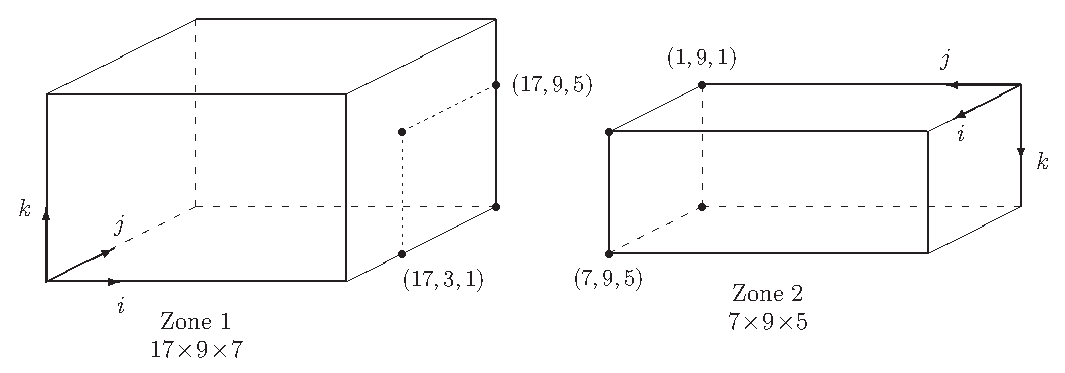
\includegraphics[width=\textwidth]{cnct.figs/cnct_1to1}
   \caption{Example Interface for 1-to-1 Connectivity}
   \label{f:cnct_1to1}
\end{figure}

\autoref{f:cnct_1to1} shows a more complex 1-to-1 abutting interface, where
the entire $j$-max face of zone 2 coincides with a subset of the $i$-max
face of zone 1.
This situation would result in the following connectivity structures:
\begin{alltt}
  GridConnectivity1to1\_t<3> Zone1/ZoneGridConnectivity/IMax =
    \{\{
    int[3] Transform = [-2,-1,-3] ;
    IndexRange\_t<3> PointRange =
      \{\{
      int[3] Begin = [17,3,1] ;
      int[3] End   = [17,9,5] ;
      \}\} ;
    IndexRange\_t<3> PointRangeDonor =
      \{\{
      int[3] Begin = [7,9,5] ; 
      int[3] End   = [1,9,1] ;
      \}\} ;
    Identifier(Zone\_t) ZoneDonorName = Zone2 ;
    \}\} ;
\end{alltt}

\begin{alltt}
  GridConnectivity1to1\_t<3> Zone2/ZoneGridConnectivity/JMax =
    \{\{
    int[3] Transform = [-2,-1,-3] ;
    IndexRange\_t<3> PointRange =
      \{\{
      int[3] Begin = [1,9,1] ;
      int[3] End   = [7,9,5] ;
      \}\} ;
    IndexRange\_t<3> PointRangeDonor =
      \{\{
      int[3] Begin = [17,9,5] ; 
      int[3] End   = [17,3,1] ;
      \}\} ;
    Identifier(Zone\_t) ZoneDonorName = Zone1 ;
    \}\} ;
\end{alltt}
\end{example}
This example also assumes zones 1 and 2 have the identifiers |Zone1| and
|Zone2|, respectively.
Note that the index transformation matrix for both this and the previous
examples is symmetric; hence, the value of |Transform| is identical for
both members of the interface pair.
In general this will not always be the case.

\subsection{General Interface Connectivity Structure Definition: \texttt{GridConnectivity\_t}}
\label{s:GridConnectivity}

|GridConnectivity_t| contains connectivity information for generalized
multizone interfaces, and may be used for any mix of structured and
unstructured zones.
Its purpose is to describe mismatched-abutting and overset interfaces,
but can also be used for 1-to-1 abutting interfaces.

For abutting interfaces that are not 1-to-1, also referred to as patched
or mismatched, an interface patch is the subrange of the face of a zone
that touches one and only one other zone.
This structure identifies the subrange of indices (or array of indices)
that make up the interface and gives their image in the adjacent (donor)
zone.
It also identifies the name of the adjacent zone.
If a given face of a zone touches several (say $N$) adjacent zones,
then $N$ different instances of |GridConnectivity_t| are needed to
describe all the interfaces.
For a single abutting interface, two instances of |GridConnectivity_t|
are needed in the database -- one for each adjacent zone.

For overset interfaces, this structure identifies the fringe points of
a given zone that lie in one and only one other zone.  If the fringe
points of a zone lie in several (say $N$) overlapping zones, then $N$
different instances of |GridConnectivity_t| are needed to describe the
overlaps.  It is possible with overset grids that a single fringe point
may actually lie in several overlapping zones (though in typical usage,
linkage to only one of the overlapping zones is kept).  There is no
restriction against a given fringe point being contained within multiple
instances of |GridConnectivity_t|; therefore, this structure allows the
description of a single fringe point lying in several overlapping zones.

\begin{alltt}
  GridConnectivityType\_t := Enumeration(
    GridConnectivityTypeNull,
    GridConnectivityTypeUserDefined,
    Overset,
    Abutting,
    Abutting1to1 ) ;

  GridConnectivity\_t< int IndexDimension, int CellDimension > :=
    \{
    List( Descriptor\_t Descriptor1 ... DescriptorN ) ;                      (o)

    GridConnectivityType\_t GridConnectivityType ;                           (o/d)

    GridLocation\_t GridLocation ;                                           (o/d)

    IndexRange\_t<IndexDimension> PointRange ;                               (o:r)
    IndexArray\_t<IndexDimension, PointListSize, int>  PointList ;           (r:o)
    IndexArray\_t<IndexDimension, PointListSize, int>  PointListDonor ;      (o)
    IndexArray\_t<IndexDimension, PointListSize, int>  CellListDonor ;       (o)

    Identifier(Zone\_t) ZoneDonorName ;                                      (r)

    DataArray\_t <real, 2, [CellDimension, PointListSize]> InterpolantsDonor (o)

    GridConnectivityProperty\_t GridConnectivityProperty ;                   (o)

    List( UserDefinedData\_t UserDefinedData1 ... UserDefinedDataN ) ;       (o)

    int Ordinal ;                                                           (o)
    \} ;
\end{alltt}

\begin{notes}
\item Default names for the \texttt{Descriptor\_t} and
      \texttt{UserDefinedData\_t} lists are as shown; users may choose
      other legitimate names.
      Legitimate names must be unique within a given instance of
      \texttt{GridConnectivity\_t} and shall not include the names
      \texttt{CellListDonor}, \texttt{GridConnectivityProperty},
      \texttt{GridConnectivityType}, \texttt{GridLocation},
      \texttt{InterpolantsDonor}, \texttt{Ordinal}, \texttt{PointList},
      \texttt{PointListDonor}, or \texttt{PointRange}.
\item \texttt{ZoneDonorName} must be equated to a zone identifier
      within the current CGNS database (i.e., it must be equal to one
      of the \texttt{Zone\_t} identifiers contained in the current
      \texttt{CGNSBase\_t} entity).
\item If \texttt{GridConnectivityType} is absent, then its default value
      is \texttt{Overset}.
\item For \texttt{Abutting} or \texttt{Abutting1to1} interfaces,
      \texttt{GridLocation} can be either \texttt{Vertex} or
      \texttt{FaceCenter}.
      When \texttt{GridLocation} is set to \texttt{Vertex}, then
      \texttt{PointList} or \texttt{PointRange} refer to node indices,
      for both structured and unstructured grids.
      When \texttt{GridLocation} is set to \texttt{FaceCenter}, then
      \texttt{PointList} or \texttt{PointRange} refer to face elements.
      Face elements are indexed using different methods depending if the
      zone is structured or unstructured.
      For a structured zone, face elements are indexed using the
      minimum of the connecting vertex indices, as described in
      \autoref{s:structgrid}.
      For an unstructured zone, face elements are indexed using their
      element numbering, as defined in the \texttt{Elements\_t} data
      structures.
      For \texttt{Overset} interfaces, \texttt{GridLocation} can be
      either \texttt{Vertex} or \texttt{CellCenter}, allowing the
      description of the overlap region in the receiver zone to be
      consistent with the grid location used for storing the flow
      solution.
      If \texttt{GridLocation} is absent, then its default value is
      \texttt{Vertex}.
\item One of \texttt{PointRange} and \texttt{PointList} must be
      specified, but not both.
\item If \texttt{PointRange} is specified, then an index ordering
      convention is needed to map receiver-zone grid points to
      donor-zone grid points.
      FORTRAN multidimensional array ordering is used.
\item If \texttt{GridConnectivityType} is \texttt{Abutting1to1} or
      \texttt{Abutting}, then \texttt{PointRange} or \texttt{PointList}
      must define points associated with a face subrange (if
      the zone is structured, all points must be in a single
      computational grid plane); the donor-zone grid locations defined
      by \texttt{PointListDonor} or \texttt{CellListDonor} must also be
      associated with a face subrange.
\item If donor information is given, either \texttt{PointListDonor}
      alone, or \texttt{CellListDonor} with or without
      \texttt{InterpolantsDonor}, must be used.
      Either \texttt{PointListDonor} alone, or \texttt{CellListDonor}
      plus \texttt{InterpolantsDonor}, must be used.
      The use of \texttt{PointListDonor} is restricted to
      \texttt{Abutting1to1}, whereas \texttt{CellListDonor} can be used
      for any interface type.
\item Thus, for a \texttt{GridConnectivityType} that is not
      \texttt{Abutting1to1}, there are three allowable levels of
      description concerning the connectivity information: (a) full,
      giving \texttt{ZoneDonorName} with \texttt{CellListDonor}
      plus \texttt{InterpolantsDonor}; (b) partial, giving
      \texttt{ZoneDonorName} with \texttt{CellListDonor} but
      no \texttt{InterpolantsDonor}; or (c) minimal, giving
      \texttt{ZoneDonorName} only.
\end{notes}

The type of multizone interface connectivity may be \fort{Overset},
\fort{Abutting}, or \fort{Abutting1to1}.
\fort{Overset} refers to zones that overlap; for a 3-D configuration the
overlap is a 3-D region.
|Abutting| refers to zones that abut or touch, but do not overlap (other
than the vertices and faces that make up the interface).
|Abutting1to1| is a special case of abutting interfaces where grid lines
are continuous across the interface and all vertices on the interface
are shared by the two adjacent zones.
See \autoref{s:interface_types} for a description of the three different
types of interfaces.

The interface grid points within the receiver zone may be specified by
|PointRange| if they constitute a logically rectangular region (e.g., an
abutting interface where an entire face of the receiver zone abuts with a
part of a face of the donor zone).  In all other cases, |PointList| should be
used to list the receiver-zone grid points making up the interface.
For a structured-to-structured interface, all indices in |PointRange| or
|PointList| should have one index element in common (see note 7).

\texttt{GridLocation} identifies the location of indices within the
receiver zone described by \texttt{PointRange} or \texttt{PointList}.
It also identifies the location of indices defined by
\texttt{PointListDonor} in the donor zone.
\texttt{GridLocation} does \emph{not} apply to \texttt{CellListDonor} or 
\texttt{InterpolantsDonor}.
The \texttt{CellListDonor} is always an index or indices that define a
particular cell or element, while the \texttt{InterpolantsDonor} defines
an interpolation value relative to the cell/element \emph{vertices}.
In other words, when using \texttt{InterpolantsDonor}, the interpolants
are always given with respect to the vertices of the donor zone.
\texttt{InterpolantsDonor} is currently only defined for structured
grids and certain basic unstructured grid element types.

For structured grids, the interpolant value is given along each index
direction, depending on the location within the cell.
For example, if the point is located within the cell at a position 75\%
in the $i$-direction, 41\% in the $j$-direction, and 20\% in the
$k$-direction, then \texttt{InterpolantsDonor} values ($r$, $s$, $t$)
would be (0.75, 0.41, 0.20).

The interpolation function is a linear combination of the $x$, $y$, and
$z$ values at the surrounding nodes:
$$
d = \sum_{i=1}^{N} W_i \cdot d_i
$$
where $d$ is the $x$, $y$, or $z$ value at an interior point in the
cell, $d_i$ is the $x$, $y$, or $z$ value at node $i$, and $W_i$ is a
weight at node $i$.
The weights are functions of the parametric variables $r$, $s$, and $t$
(corresponding with the $i$, $j$, and $k$ directions, respectively),
which vary from 0 to 1, inclusively.
For structured grids in 3-D, $N = 8$.
Note that for skewed, non-parallel grids, it is not always easy to
determine the interpolants geometrically, and it may be necessary to
solve an inverse problem using the interpolation function.

{\centering%
\begin{minipage}[t]{0.55\linewidth}
   \centering
   \vspace{0pt}
   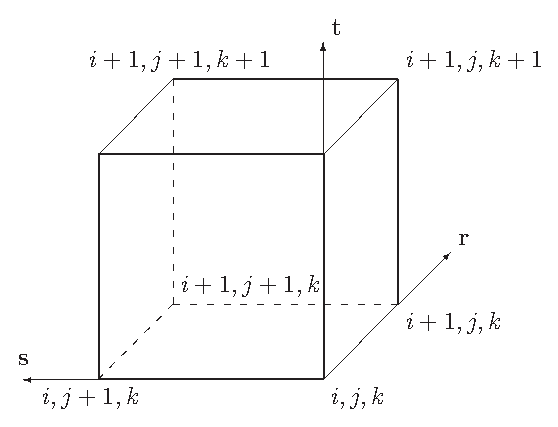
\includegraphics{cnct.figs/cnct_struct}
\end{minipage}%
\begin{minipage}[t]{0.45\linewidth}
   \vspace{-\abovedisplayskip}
   \begin{eqnarray*}
      W_{i,  j,  k  } &=& (1-r)(1-s)(1-t) \\
      W_{i+1,j,  k  } &=& r(1-s)(1-t) \\
      W_{i,  j+1,k  } &=& (1-r)s(1-t) \\
      W_{i,  j,  k+1} &=& (1-r)(1-s)t \\
      W_{i+1,j+1,k  } &=& rs(1-t) \\
      W_{i+1,j,  k+1} &=& r(1-s)t \\
      W_{i,  j+1,k+1} &=& (1-r)st \\
      W_{i+1,j+1,k+1} &=& rst
   \end{eqnarray*}
\end{minipage}}
\vspace{\baselineskip}

For unstructured grids, \texttt{InterpolantsDonor} is defined only for
the basic linear element types:
\texttt{BAR\_2}, \texttt{TRI\_3}, \texttt{QUAD\_4}, \texttt{TETRA\_4},
\texttt{PYRA\_5}, \texttt{PENTA\_6}, and \texttt{HEXA\_8}, defined in
\autoref{s:unstructgrid}.
The directionality for the $r$, $s$, and $t$ interpolants for the basic
element types is defined as follows.

\vspace{\baselineskip}
\texttt{BAR\_2}\\[-2\baselineskip]
\begin{center}
\begin{minipage}[t]{0.5\linewidth}
   \centering
   \vspace{0pt}
   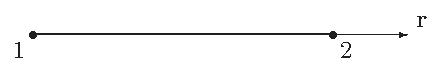
\includegraphics{cnct.figs/cnct_unst_bar2}
\end{minipage}%
\begin{minipage}[t]{0.5\linewidth}
   \vspace{-\abovedisplayskip}
   \begin{eqnarray*}
      W_1 &=& 1-r \\
      W_2 &=& r
   \end{eqnarray*}
\end{minipage}
\end{center}

\newpage
%\vspace{\baselineskip}
\texttt{TRI\_3}\\[-2\baselineskip]
\begin{center}
\begin{minipage}[t]{0.5\linewidth}
   \centering
   \vspace{0pt}
   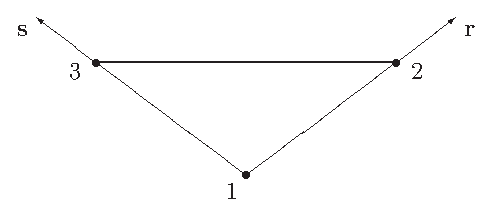
\includegraphics{cnct.figs/cnct_unst_tri3}
\end{minipage}%
\begin{minipage}[t]{0.5\linewidth}
   \vspace{-\abovedisplayskip}
   \begin{eqnarray*}
      W_1 &=& 1-r-s \\
      W_2 &=& r \\
      W_3 &=& s
   \end{eqnarray*}
\end{minipage}
\end{center}

\vspace{\baselineskip}
\texttt{QUAD\_4}\\[-2\baselineskip]
\begin{center}
\begin{minipage}[t]{0.5\linewidth}
   \centering
   \vspace{0pt}
   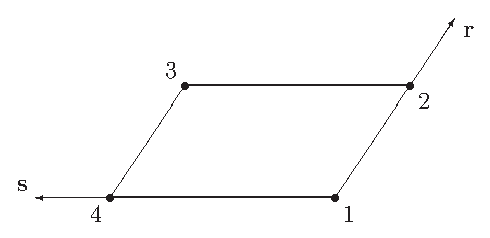
\includegraphics{cnct.figs/cnct_unst_quad4}
\end{minipage}%
\begin{minipage}[t]{0.5\linewidth}
   \vspace{-\abovedisplayskip}
   \begin{eqnarray*}
      W_1 &=& (1-r)(1-s) \\
      W_2 &=& r(1-s) \\
      W_3 &=& rs \\
      W_4 &=& (1-r)s
   \end{eqnarray*}
\end{minipage}
\end{center}

\vspace{\baselineskip}
\texttt{TETRA\_4}\\[-2\baselineskip]
\begin{center}
\begin{minipage}[t]{0.5\linewidth}
   \centering
   \vspace{0pt}
   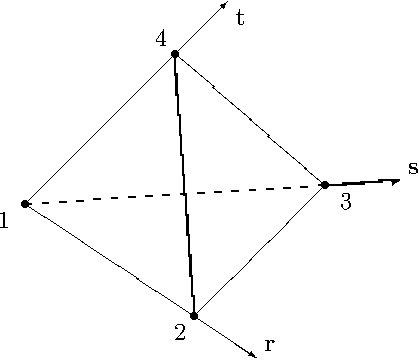
\includegraphics{cnct.figs/cnct_unst_tetra4}
\end{minipage}%
\begin{minipage}[t]{0.5\linewidth}
   \vspace{-\abovedisplayskip}
   \begin{eqnarray*}
      W_1 &=& 1-r-s-t \\
      W_2 &=& r \\
      W_3 &=& s \\
      W_4 &=& t
   \end{eqnarray*}
\end{minipage}
\end{center}

\newpage
%\vspace{\baselineskip}
\texttt{PYRA\_5}\\[-2\baselineskip]
\begin{center}
\begin{minipage}[t]{0.5\linewidth}
   \centering
   \vspace{0pt}
   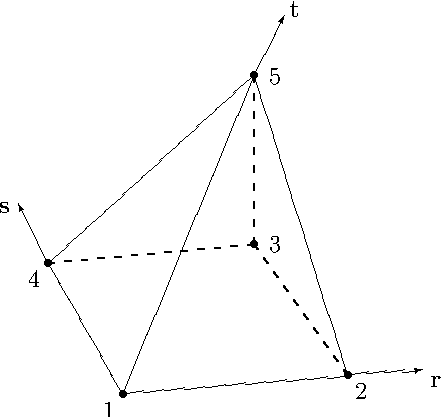
\includegraphics{cnct.figs/cnct_unst_pyra5}
\end{minipage}%
\begin{minipage}[t]{0.5\linewidth}
   \vspace{-\abovedisplayskip}
   \begin{eqnarray*}
      W_1 &=& (1-r)(1-s)(1-t) \\
      W_2 &=& r(1-s)(1-t) \\
      W_3 &=& rs(1-t) \\
      W_4 &=& (1-r)s(1-t) \\
      W_5 &=& t
   \end{eqnarray*}
\end{minipage}
\end{center}

\vspace{\baselineskip}
\texttt{PENTA\_6}\\[-2\baselineskip]
\begin{center}
\begin{minipage}[t]{0.5\linewidth}
   \centering
   \vspace{0pt}
   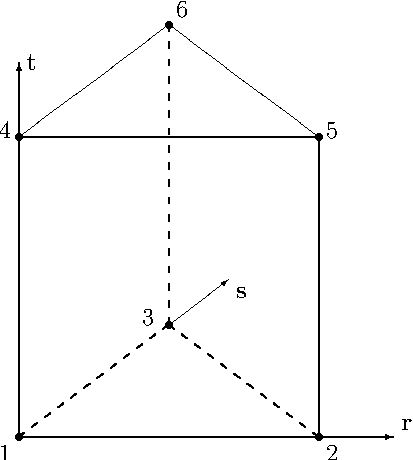
\includegraphics{cnct.figs/cnct_unst_penta6}
\end{minipage}%
\begin{minipage}[t]{0.5\linewidth}
   \vspace{-\abovedisplayskip}
   \begin{eqnarray*}
      W_1 &=& (1-r-s)(1-t) \\
      W_2 &=& r(1-t) \\
      W_3 &=& s(1-t) \\
      W_4 &=& (1-r-s)t \\
      W_5 &=& rt \\
      W_6 &=& st
   \end{eqnarray*}
\end{minipage}
\end{center}

\newpage
%\vspace{\baselineskip}
\texttt{HEXA\_8}\\[-2\baselineskip]
\begin{center}
\begin{minipage}[t]{0.5\linewidth}
   \centering
   \vspace{0pt}
   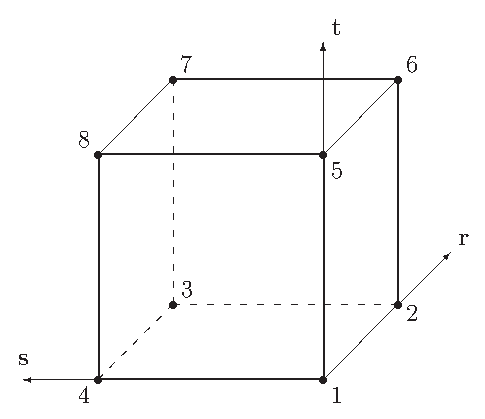
\includegraphics{cnct.figs/cnct_unst_hexa8}
\end{minipage}%
\begin{minipage}[t]{0.5\linewidth}
   \vspace{-\abovedisplayskip}
   \begin{eqnarray*}
      W_1 &=& (1-r)(1-s)(1-t) \\
      W_2 &=& r(1-s)(1-t) \\
      W_3 &=& rs(1-t) \\
      W_4 &=& (1-r)s(1-t) \\
      W_5 &=& (1-r)(1-s)t \\
      W_6 &=& r(1-s)t \\
      W_7 &=& rst \\
      W_8 &=& (1-r)st
   \end{eqnarray*}
\end{minipage}
\end{center}

\fort{PointListDonor} may only be used when the interface is
\fort{Abutting1to1}.
It contains the images of all the receiver-zone interface points in the
donor zone.
If the zone is structured, all indices in \fort{PointListDonor}
should have one index element in common.

For mismatched or overset interfaces, the zone connectivity
donor information, when given, is defined using either the
\fort{CellListDonor} alone, or the combination of \texttt{CellListDonor}
and \texttt{InterpolantsDonor}.
\fort{CellListDonor} contains the list of donor cells or elements in
which each node of the receiver zone can be located.
\fort{InterpolantsDonor} contains the interpolation factors to locate
the receiver nodes in the donor cells.
\fort{InterpolantsDonor} may be thought of as bi- or tri-linear
interpolants (depending on \fort{CellDimension}) in the cell of the
donor zone.

A \fort{GridConnectivityProperty\_t} data structure, described in
\autoref{s:GridConnectivityProperty}, may be used to record special
properties associated with particular connectivity patches, such as a
periodic interface, or an interface where data is to be averaged in some
way.

The \fort{UserDefinedData\_t} data structure allows arbitrary
user-defined data to be stored in \fort{Descriptor\_t} and
\fort{DataArray\_t} children without the restrictions or implicit
meanings imposed on these node types at other node locations.

|Ordinal| is user-defined and has no restrictions on the values that it can
contain.  It is included for backward compatibility to assist implementation
of the CGNS system into applications whose I/O depends heavily on the
numbering of zone interfaces.  Since there are no restrictions on the values
contained in |Ordinal| (or that |Ordinal| is even provided), there is no
guarantee that the interfaces for a given zone in an existing CGNS database
will have sequential values from 1 to $N$ without holes or repetitions.  Use
of |Ordinal| is discouraged and is on a user-beware basis.

\subsubsection*{FUNCTION \texttt{PointListSize}:}

\noindent return value: |int| \\
\noindent dependencies: |PointRange|, |PointList|

\fort{PointListDonor}, \fort{CellListDonor}, and \fort{InterpolantsDonor}
require the function \fort{PointListSize}, to identify the length of the
array.
If \fort{PointRange} is specified by \fort{GridConnectivity\_t},
then \fort{PointListSize} is obtained from the number of grid points
(inclusive) between the beginning and ending indices of \fort{PointRange}.
If \fort{PointList} is specified by \fort{GridConnectivity\_t},
then \fort{PointListSize} is actually a user input during creation of
the database; it is the length of the array \fort{PointList} whose
elements are also user inputs (by ``user'' we mean the application code
that is generating the CGNS database).

By definition, the |PointList| and |PointListDonor| arrays have the
same size, and this size should be stored along with the arrays in
their respective |IndexArray_t| structures.
|PointListSize| was chosen to be a structure function, rather than a
separate element of |GridConnectivity_t| for the following reasons:
first, it is redundant if |PointRange| is specified; and second, it
leads to redundant storage if |PointList| is specified, since the value
of |PointListSize| is also stored within the |PointList| structure.

This situation has somewhat of a precedent within the SIDS definitions.
The structure \fort{Descriptor\_t} contains a string of unspecified length.
Yet in  actual implementation, the (string) length is a function of the
descriptor string itself and should be stored along with the string.

\subsection{General Interface Connectivity Examples}
\label{s:cnct_gen_example}

\begin{example}{Structured Abutting Zones}
\label{ex:struct_abut}

Say that you have a three-dimensional structured grid.
Assume that at the interface between two zones you have the 
situation shown in \autoref{f:cnct_example1}.

\begin{figure}[!htb]
   \centering
   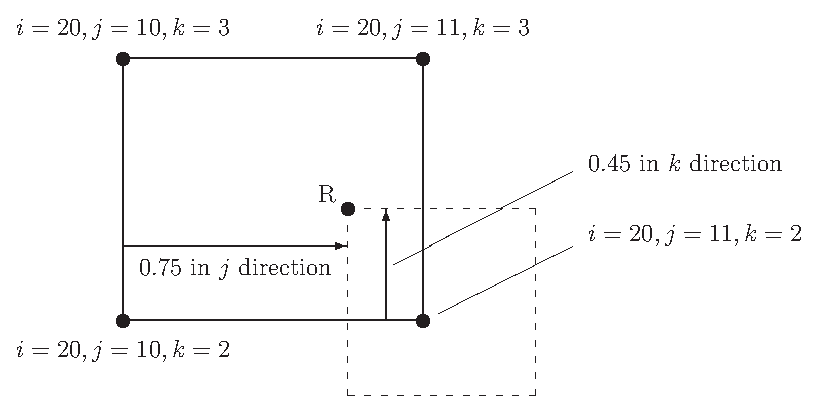
\includegraphics{cnct.figs/cnct_example1}
   \caption{Example Interface for Generalized Connectivity, Structured Grids}
   \label{f:cnct_example1}
\end{figure}

In this particular example, the patching occurs on a ``plane''.
In other words, the two cells in 3-D have faces that abut in a 2-D
sense.
It is these faces that we are picturing here.
The solid quadrilateral is the donor cell face, and the dashed
quadrilateral is the position of the receiving cell face relative to the
donor cell.
Note that since this is a 2-D-type of abutting case, one of the indices
(in this case $i = 20$, which represents \texttt{imax}) of the
donor cell is constant.
For this example, the point R of the receiver cell is located within the
donor cell pictured, and we wish to give the \texttt{CellListDonor} and
\texttt{InterpolantsDonor} for it.

Because this is a structured grid, the \texttt{CellListDonor} in this
case is given by
\begin{alltt}
   CellListDonor = (19, 10, 2)
\end{alltt}

Here, we are using the ``Structured Grid Notation and Indexing
Conventions'' (see \autoref{s:structgrid}) that say cell centers, face
centers, and edge centers are indexed by the minimum $i$, $j$, and $k$
indices of the connecting vertices.

The \texttt{InterpolantsDonor} defines an interpolation value relative
to the cell/element vertices.
In this case, say that the point R is located 0.75 along the
$j$-index direction and 0.45 along the $k$-index direction.
(It also lies on the $i = 20$, or \texttt{imax} face.)
Thus, in this example:
\begin{alltt}
   InterpolantsDonor = (1.0, 0.75, 0.45) 
\end{alltt}
Note that if the donor zone was instead located on an $i = 1$
(\texttt{imin} face), then the \texttt{CellListDonor} would be (1, 10, 2)
and the \texttt{InterpolantsDonor} would be (0.0, 0.75, 0.45).
\end{example}

\begin{example}{Unstructured Abutting Zones, \texttt{HEXA\_8} Donor Cell}
\label{ex:unstruct_abut1}

As a second example, assume that you have the same setup as before, but
now with a three-dimensional unstructured grid, shown in
\autoref{f:cnct_example2}.
In this case, we no longer have a 3-D array of indices defining
coordinate directions.
Instead, we simply have a 1-D list of indices as well as a list of
volume (and possibly face) elements composed of those indices.
In this example we again are assuming the two zones abut in a 2-D sense.
We now have the choice of describing the donor in terms of its volume
element or its boundary (face) element, if available.
Here in this example, we use the volume element.

\begin{figure}[!htb]
   \centering
   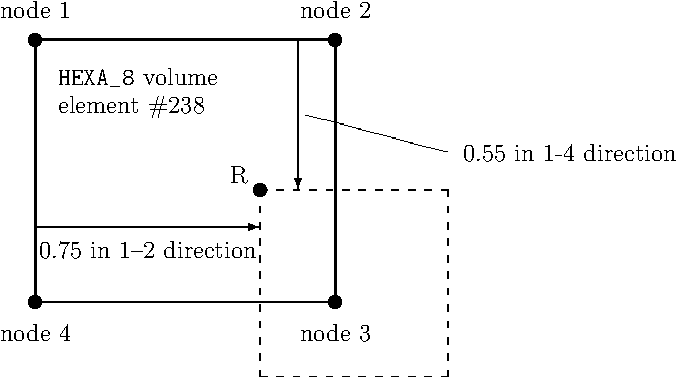
\includegraphics{cnct.figs/cnct_example2}
   \caption{Example Interface for Generalized Connectivity, Unstructured
            Grids with \texttt{HEXA\_8} Donor Cell}
   \label{f:cnct_example2}
\end{figure}

The \texttt{HEXA\_8} volume element has been appropriately numbered,
using the ``Unstructured Grid Element Numbering Conventions'' defined in
\autoref{s:unstructgrid}.
In this example, it is the 1-2-3-4 face of the volumetric element that
is abutting with the other zone (but it could be any of its six faces)

The \texttt{CellListDonor} in this case is simply given by
\begin{alltt}
   CellListDonor = (238)
\end{alltt}
Using the convention established above for \texttt{HEXA\_8} elements, the
\texttt{InterpolantsDonor} would be
\begin{alltt}
   InterpolantsDonor = (0.75, 0.55, 0.0)
\end{alltt}
\end{example}

\begin{example}{Unstructured Abutting Zones, \texttt{TRI\_3} Donor Cell}
\label{ex:unstruct_abut2}

As a third example, assume that you have two zones in a
three-dimensional unstructured grid with triangles and quadrilaterals at
its boundaries, as shown in \autoref{f:cnct_example3}.
Here the current zone (made up of quadrilateral faces) is abutting the
donor zone (made up of triangular faces) in a 2-D sense.
We again have the choice of describing the donor in terms of its volume
element or its boundary (face) element.
Here in this example, we use the face element.

\begin{figure}[!htb]
   \centering
   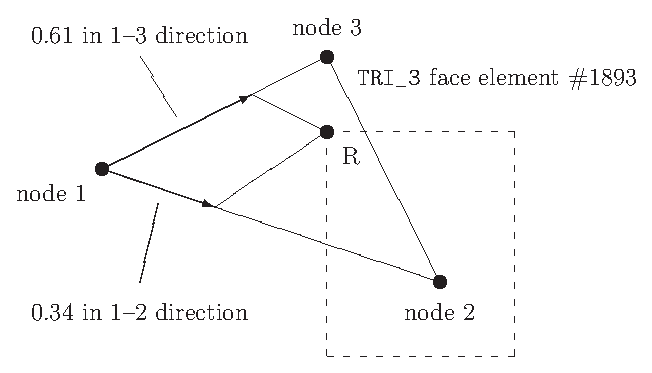
\includegraphics{cnct.figs/cnct_example3}
   \caption{Example Interface for Generalized Connectivity, Unstructured
            Grids with \texttt{TRI\_3} Donor Cell}
   \label{f:cnct_example3}
\end{figure}

The \texttt{CellListDonor} in this case is simply given by
\begin{alltt}
   CellListDonor = (1893)
\end{alltt}
Using the convention established above for \texttt{TRI\_3} elements, the
\texttt{InterpolantsDonor} would be:
\begin{alltt}
   InterpolantsDonor = (0.34, 0.61)
\end{alltt}
In this case the third dimension of the \texttt{InterpolantsDonor}
(although present) is not used, because by default the interpolation is
only two-dimensional in the 2-D plane of the donor face.
\end{example}

\subsection{Grid Connectivity Property Structure Definition: \texttt{GridConnectivityProperty\_t}}
\label{s:GridConnectivityProperty}

\fort{GridConnectivityProperty\_t} allows the recording of special
properties associated with particular connectivity patches.
At the current time, only two properties (\fort{Periodic\_t} and
\fort{AverageInterface\_t}) are included, but extensions involving
other properties may be implemented as additional nodes under
\fort{GridConnectivityProperty\_t} in the future.

\begin{alltt}
  GridConnectivityProperty\_t :=
    \{
    List( Descriptor\_t Descriptor1 ... DescriptorN ) ;                      (o)

    Periodic\_t Periodic ;                                                   (o)

    AverageInterface\_t AverageInterface ;                                   (o)

    List( UserDefinedData\_t UserDefinedData1 ... UserDefinedDataN ) ;       (o)
    \} ;
\end{alltt}

\begin{notes}
\item
 Default names for the \fort{Descriptor\_t} and
 \fort{UserDefinedData\_t}
 lists are as shown; users may choose other legitimate names.
 Legitimate names must be unique within a given instance of
 \fort{GridConnectivityProperty\_t} and shall not include the names
 \fort{Periodic} or \fort{AverageInterface}.
\end{notes}

The \fort{Periodic\_t} and \fort{AverageInterface\_t} data structures
may be used to record properties associated with periodic interfaces, or
interfaces where data is to be averaged in some way, respectively.

The \fort{UserDefinedData\_t} data structure allows arbitrary
user-defined data to be stored in \fort{Descriptor\_t} and
\fort{DataArray\_t} children without the restrictions or implicit
meanings imposed on these node types at other node locations.

\subsubsection{Periodic Interface Structure Definition: \texttt{Periodic\_t}}
\label{s:Periodic}

The \fort{Periodic\_t} data structure allows data associated with
a periodic interface to be recorded.

\begin{alltt}
  Periodic\_t :=
    \{
    List( Descriptor\_t Descriptor1 ... DescriptorN ) ;                      (o)

    DataArray\_t<real, 1, PhysicalDimension> RotationCenter ;                (r)
    DataArray\_t<real, 1, PhysicalDimension> RotationAngle ;                 (r)
    DataArray\_t<real, 1, PhysicalDimension> Translation ;                   (r)

    DataClass\_t DataClass ;                                                 (o)

    DimensionalUnits\_t DimensionalUnits ;                                   (o)

    List( UserDefinedData\_t UserDefinedData1 ... UserDefinedDataN ) ;       (o)
    \} ;
\end{alltt}

\begin{notes}
\item
 Default names for the \fort{Descriptor\_t} and
 \fort{UserDefinedData\_t} lists are as shown; users may choose other
 legitimate names.
 Legitimate names must be unique within a given instance of
 \fort{Periodic\_t} and shall not include the names \fort{DataClass},
 \fort{DimensionalUnits}, \fort{RotationAngle}, \fort{RotationCenter},
 or \fort{Translation}.
\end{notes}

\fort{RotationCenter} is the origin for defining the rotation angle
between the periodic interfaces.
\fort{RotationAngle} defines the angle from the current interface to
the connecting interface.
If rotating about more than one axis, the rotation is performed first
about the x-axis, then the y-axis, then the z-axis.
\fort{Translation} defines the translation from the current interface
to the connecting interface.

\fort{DataClass} defines the default for the class of data contained in
the \fort{DataArray\_t} structures.
If the data is dimensional, \fort{DimensionalUnits} may be used to
describe the system of dimensional units employed.
If present, these two entities take precedence of all corresponding
entities at higher levels of the hierarchy.
These precedence rules are further discussed in \autoref{s:precedence}.

The \fort{UserDefinedData\_t} data structure allows arbitrary
user-defined data to be stored in \fort{Descriptor\_t} and
\fort{DataArray\_t} children without the restrictions or implicit
meanings imposed on these node types at other node locations.

\subsubsection{Average Interface Structure Definition: \texttt{AverageInterface\_t}}
\label{s:AverageInterface}

The \fort{AverageInterface\_t} data structure is used when data at the
current connectivity interface is to be averaged in some way prior to
passing it to a neighboring interface.

\begin{alltt}
  AverageInterface\_t :=
    \{
    List( Descriptor\_t Descriptor1 ... DescriptorN ) ;                      (o)

    AverageInterfaceType\_t AverageInterfaceType ;                           (r)

    List( UserDefinedData\_t UserDefinedData1 ... UserDefinedDataN ) ;       (o)
    \} ;
\end{alltt}

\begin{notes}
\item
 Default names for the \fort{Descriptor\_t} and
 \fort{UserDefinedData\_t} lists are as shown; users may choose other
 legitimate names.
 Legitimate names must be unique within a given instance of
 \fort{AverageInterface\_t} and shall not include the name
 \fort{AverageInterfaceType}.
\end{notes}

\fort{AverageInterfaceType\_t} is a required enumeration data structure
that is used to define the type of averaging to be done.
\begin{alltt}
  AverageInterfaceType_t := Enumeration(
    AverageInterfaceTypeNull,
    AverageInterfaceTypeUserDefined,
    AverageAll,
    AverageCircumferential,
    AverageRadial,
    AverageI,
    AverageJ,
    AverageK ) ;
\end{alltt}

\fort{AverageAll} means that the data from the entire current patch is
averaged, whereas each of the other choices indicates averaging of the
data on the current interface in the indicated direction.
Note that \fort{AverageI}, \fort{AverageJ}, and \fort{AverageK}
apply only to structured grids.

The \fort{UserDefinedData\_t} data structure allows arbitrary
user-defined data to be stored in \fort{Descriptor\_t} and
\fort{DataArray\_t} children without the restrictions or implicit
meanings imposed on these node types at other node locations.

\subsection{Overset Grid Holes Structure Definition: \texttt{OversetHoles\_t}}
\label{s:OversetHoles}

Grid connectivity for overset grids must also include ``holes'' within zones,
where any solution states are ignored or ``turned off'', because they are
solved for in some other overlapping zone.  The structure |OversetHoles_t|
specifies those points within a given zone that make up a hole (or holes),
and applies to both structured and unstructured zones.
Grid points specified in this structure are equivalent to those with
IBLANK=0 in the PLOT3D format.

\begin{alltt}
  OversetHoles\_t< int IndexDimension > :=
    \{
    List( Descriptor\_t Descriptor1 ... DescriptorN ) ;                      (o)

    GridLocation\_t GridLocation ;                                           (o/d)

    List( IndexRange\_t<IndexDimension> 
      PointRange, PointRange2 ... PointRangeN ) ;                           (o:r)

    IndexArray\_t<IndexDimension, PointListSize, int> PointList ;            (r:o)

    List( UserDefinedData\_t UserDefinedData1 ... UserDefinedDataN ) ;       (o)
    \} ;
\end{alltt}

\begin{notes}
\item
 Default names for the \fort{Descriptor\_t}, \fort{IndexRange\_t}, and
 \fort{UserDefinedData\_t}
 lists are as shown; users may choose other legitimate names.
 Legitimate names must be unique 
 within a given instance of \fort{OversetHoles\_t} and shall not include the
 names \fort{GridLocation} or \fort{PointList}.
\item
 If |GridLocation| is absent, then its default value is |Vertex|.
\item
 One of |PointRange| and |PointList| must be specified, but not both.
\end{notes}

The location of grid indices specified in \fort{PointList} and the
\fort{PointRange} list is given by \fort{GridLocation}.

The grid points making up a hole within a zone may be specified by
|PointRange| if they constitute a logically rectangular region.  If the hole
points constitute a (small) set of possibly overlapping logically rectangular
regions, then they may be specified by the list |PointRange|, |PointRange2|,
etc.  The more general alternate is to use |PointList| to list all grid
points making up the hole(s) within a zone.
Note that using multiple |PointRange| specifications may result in a
given hole being specified more than once.

The \fort{UserDefinedData\_t} data structure allows arbitrary
user-defined data to be stored in \fort{Descriptor\_t} and
\fort{DataArray\_t} children without the restrictions or implicit
meanings imposed on these node types at other node locations.

\subsubsection*{FUNCTION \texttt{PointListSize}:}

\noindent return value: |int| \\
\noindent dependencies: |PointList|

|OversetHoles_t| requires one structure function, |PointListSize|, to 
identify the length of the |PointList| array.
|PointListSize| is a user input.
(See the discussion on function |PointListSize| in
\autoref{s:GridConnectivity}).


\clearemptydoublepage
\section{Boundary Conditions}
\label{s:bc}
\thispagestyle{plain}

\subsection{Boundary Condition Type and Location}
\label{s:bctype}

\noindent
\textit{Node}: \texttt{BC\_t}

\begin{fctbox}
\textcolor{output}{\textit{ier}} = cg\_boco\_write(\textcolor{input}{int fn}, \textcolor{input}{int B}, \textcolor{input}{int Z}, \textcolor{input}{char *boconame}, & - w m \\
~~~~~~\textcolor{input}{BCType\_t bocotype}, \textcolor{input}{PointSetType\_t ptset\_type}, \textcolor{input}{cgsize\_t npnts}, & \\
~~~~~~\textcolor{input}{cgsize\_t *pnts}, \textcolor{output}{\textit{int *BC}}); & \\
\textcolor{output}{\textit{ier}} = cg\_boco\_normal\_write(\textcolor{input}{int fn}, \textcolor{input}{int B}, \textcolor{input}{int Z}, \textcolor{input}{int BC}, & - w m \\
~~~~~~\textcolor{input}{int *NormalIndex}, \textcolor{input}{int NormalListFlag}, & \\
~~~~~~\textcolor{input}{DataType\_t NormalDataType}, \textcolor{input}{void *NormalList}); & \\
\textcolor{output}{\textit{ier}} = cg\_boco\_gridlocation\_write(\textcolor{input}{int fn}, \textcolor{input}{int B}, \textcolor{input}{int Z}, \textcolor{input}{int BC}, & - w m \\
~~~~~~\textcolor{input}{\textit{GridLocation\_t location}}); & \\
\textcolor{output}{\textit{ier}} = cg\_nbocos(\textcolor{input}{int fn}, \textcolor{input}{int B}, \textcolor{input}{int Z}, \textcolor{output}{\textit{int *nbocos}}); & r - m \\
\textcolor{output}{\textit{ier}} = cg\_boco\_info(\textcolor{input}{int fn}, \textcolor{input}{int B}, \textcolor{input}{int Z}, \textcolor{input}{int BC}, \textcolor{output}{\textit{char *boconame}}, & r - m \\
~~~~~~\textcolor{output}{\textit{BCType\_t *bocotype}}, \textcolor{output}{\textit{PointSetType\_t *ptset\_type}}, \textcolor{output}{\textit{cgsize\_t *npnts}}, & \\
~~~~~~\textcolor{output}{\textit{int *NormalIndex}}, \textcolor{output}{\textit{cgsize\_t *NormalListFlag}}, & \\
~~~~~~\textcolor{output}{\textit{DataType\_t *NormalDataType}}, \textcolor{output}{\textit{int *ndataset}}); & \\
\textcolor{output}{\textit{ier}} = cg\_boco\_read(\textcolor{input}{int fn}, \textcolor{input}{int B}, \textcolor{input}{int Z}, \textcolor{input}{int BC}, \textcolor{output}{\textit{cgsize\_t *pnts}}, & r - m \\
~~~~~~\textcolor{output}{\textit{void *NormalList}}); & \\
\textcolor{output}{\textit{ier}} = cg\_boco\_gridlocation\_read(\textcolor{input}{int fn}, \textcolor{input}{int B}, \textcolor{input}{int Z}, \textcolor{input}{int BC}, & r - m \\
~~~~~~\textcolor{output}{\textit{GridLocation\_t *location}}); & \\
\hline
call cg\_boco\_write\_f(\textcolor{input}{fn}, \textcolor{input}{B}, \textcolor{input}{Z}, \textcolor{input}{boconame}, \textcolor{input}{bocotype}, \textcolor{input}{ptset\_type}, \textcolor{input}{npnts}, & - w m \\
~~~~~\textcolor{input}{pnts}, \textcolor{output}{\textit{BC}}, \textcolor{output}{\textit{ier}}) & \\
call cg\_boco\_normal\_write\_f(\textcolor{input}{fn}, \textcolor{input}{B}, \textcolor{input}{Z}, \textcolor{input}{BC}, \textcolor{input}{NormalIndex}, \textcolor{input}{NormalListFlag}, & - w m \\
~~~~~\textcolor{input}{NormalDataType}, \textcolor{input}{NormalList}, \textcolor{output}{\textit{ier}}) & \\
call cg\_boco\_gridlocation\_write\_f(\textcolor{input}{fn}, \textcolor{input}{B}, \textcolor{input}{Z}, \textcolor{input}{BC}, \textcolor{input}{location}, \textcolor{output}{\textit{ier}}); & - w m \\
call cg\_nbocos\_f(\textcolor{input}{fn}, \textcolor{input}{B}, \textcolor{input}{Z}, \textcolor{output}{\textit{nbocos}}, \textcolor{output}{\textit{ier}}) & r - m \\
call cg\_boco\_info\_f(\textcolor{input}{fn}, \textcolor{input}{B}, \textcolor{input}{Z}, \textcolor{input}{BC}, \textcolor{output}{\textit{boconame}}, \textcolor{output}{\textit{bocotype}}, \textcolor{output}{\textit{ptset\_type}}, & r - m \\
~~~~~\textcolor{output}{\textit{npnts}}, \textcolor{output}{\textit{NormalIndex}}, \textcolor{output}{\textit{NormalListFlag}}, \textcolor{output}{\textit{NormalDataType}}, \textcolor{output}{\textit{ndataset}}, & \\
~~~~~\textcolor{output}{\textit{ier}}) & \\
call cg\_boco\_read\_f(\textcolor{input}{fn}, \textcolor{input}{B}, \textcolor{input}{Z}, \textcolor{input}{BC}, \textcolor{output}{\textit{pnts}}, \textcolor{output}{\textit{NormalList}}, \textcolor{output}{\textit{ier}}) & r - m \\
call cg\_boco\_gridlocation\_read\_f(\textcolor{input}{fn}, \textcolor{input}{B}, \textcolor{input}{Z}, \textcolor{input}{BC}, \textcolor{output}{\textit{location}}, \textcolor{output}{\textit{ier}}); & r - m \\
\end{fctbox}

\noindent
\textbf{\textcolor{input}{Input}/\textcolor{output}{\textit{Output}}}

\begin{Ventryi}{\texttt{NormalListFlag}}\raggedright
\item [\texttt{fn}]
      CGNS file index number.
      (\textcolor{input}{Input})
\item [\texttt{B}]
      Base index number, where $1 \leq \text{\texttt{B}} \leq \text{\texttt{nbases}}$.
      (\textcolor{input}{Input})
\item [\texttt{Z}]
      Zone index number, where $1 \leq \text{\texttt{Z}} \leq \text{\texttt{nzones}}$.
      (\textcolor{input}{Input})
\item [\texttt{BC}]
      Boundary condition index number, where $1 \leq \text{\texttt{BC}} \leq \text{\texttt{nbocos}}$.
      (\textcolor{input}{Input} for \texttt{cg\_boco\_normal\_write},
      \texttt{cg\_boco\_info}, \texttt{cg\_boco\_read};
      \textcolor{output}{\textit{output}} for \texttt{cg\_boco\_write})
\item [\texttt{nbocos}]
      Number of boundary conditions in zone \texttt{Z}.
      (\textcolor{output}{\textit{Output}})
\item [\texttt{boconame}]
      Name of the boundary condition.
      (\textcolor{input}{Input} for \texttt{cg\_boco\_write};
      \textcolor{output}{\textit{output}} for \texttt{cg\_boco\_info})
\item [\texttt{bocotype}]
      Type of boundary condition defined.
      See the eligible types for \texttt{BCType\_t} in \autoref{s:typedefs}.
      Note that if \texttt{bocotype} is \texttt{FamilySpecified}
      the boundary condition type is being specified for the family
      to which the boundary belongs.
      The boundary condition type for the family may be read and written
      using \texttt{cg\_fambc\_read} and \texttt{cg\_fambc\_write},
      as described in \autoref{s:familybc}.
      (\textcolor{input}{Input} for \texttt{cg\_boco\_write};
      \textcolor{output}{\textit{output}} for \texttt{cg\_boco\_info})
\item [\texttt{ptset\_type}]
      The extent of the boundary condition may be defined using a range
      of points or elements using \texttt{PointRange}, or using a
      discrete list of all points or elements at which the boundary
      condition is applied using \texttt{PointList}.

      When the boundary condition is to be applied anywhere other than points,
      then \texttt{GridLocation\_t} under the \texttt{BC\_t} node must
      be used to indicate this.
      The value of \texttt{GridLocation\_t} may be read or written by
      \texttt{cg\_boco\_gridlocation\_read} and
      \texttt{cg\_boco\_gridlocation\_write}.
      As in previous versions of the library, this may also be done by
      first using \texttt{cg\_goto} (\autoref{s:navigating})
      to access the \texttt{BC\_t} node, then using
      \texttt{cg\_gridlocation\_read} or
      \texttt{cg\_gridlocation\_write} (\autoref{s:gridlocation}).
      (\textcolor{input}{Input} for \texttt{cg\_boco\_write};
      \textcolor{output}{\textit{output}} for \texttt{cg\_boco\_info})
\item [\texttt{npnts}]
      Number of points or elements defining the boundary
      condition region.
      For a \texttt{ptset\_type} of \texttt{PointRange},
      \texttt{npnts} is always two.
      For a \texttt{ptset\_type} of \texttt{PointList},
      \texttt{npnts} is the number of points or elements in the list.
      (\textcolor{input}{Input} for \texttt{cg\_boco\_write};
      \textcolor{output}{\textit{output}} for \texttt{cg\_boco\_info})
\item [\texttt{pnts}]
      Array of point or element indices defining the boundary condition
      region.
      There should be \texttt{npnts} values, each of dimension
      \texttt{IndexDimension} (i.e., 1 for unstructured grids,
      and 2 or 3 for structured grids with 2-D or 3-D elements,
      respectively).
      (\textcolor{input}{Input} for \texttt{cg\_boco\_write};
      \textcolor{output}{\textit{output}} for \texttt{cg\_boco\_read})
\item [\texttt{NormalIndex}]
      Index vector indicating the computational coordinate direction
      of the boundary condition patch normal.
      (\textcolor{input}{Input} for \texttt{cg\_boco\_normal\_write};
      \textcolor{output}{\textit{output}} for \texttt{cg\_boco\_info})
\item [\texttt{NormalListFlag}]
      For \texttt{cg\_boco\_normal\_write}, \texttt{NormalListFlag} is a
      flag indicating if the normals are defined in \texttt{NormalList};
      1 if they are defined, 0 if they're not.

      For \texttt{cg\_boco\_info}, if the normals are defined in
      \texttt{NormalList}, \texttt{NormalListFlag} is the number of points
      in the patch times \texttt{phys\_dim}, the number of coordinates
      required to define a vector in the field.
      If the normals are not defined in \texttt{NormalList},
      \texttt{NormalListFlag} is 0.
      (\textcolor{input}{Input} for \texttt{cg\_boco\_normal\_write};
      \textcolor{output}{\textit{output}} for \texttt{cg\_boco\_info})
\item [\texttt{NormalDataType}]
      Data type used in the definition of the normals.
      Admissible data types for the normals are \texttt{RealSingle} and
      \texttt{RealDouble}.
      (\textcolor{input}{Input} for \texttt{cg\_boco\_normal\_write};
      \textcolor{output}{\textit{output}} for \texttt{cg\_boco\_info})
\item [\texttt{NormalList}]
      List of vectors normal to the boundary condition patch pointing
      into the interior of the zone.
      (\textcolor{input}{Input} for \texttt{cg\_boco\_normal\_write};
      \textcolor{output}{\textit{output}} for \texttt{cg\_boco\_read})
\item [\texttt{ndataset}]
      Number of boundary condition datasets for the current boundary
      condition.
      (\textcolor{output}{\textit{Output}})
\item [\texttt{location}]
      Grid location used in the definition of the point set.
      The currently admissible locations are \texttt{Vertex} (the default
      if not given). For 2-D grids, \texttt{EdgeCenter} is also allowed,
      and for 3-D grids, the additional values of \texttt{FaceCenter},
      \texttt{IFaceCenter}, \texttt{JFaceCenter}, and
      \texttt{KFaceCenter} may be used.
      (\textcolor{input}{Input} for \texttt{cg\_boco\_gridlocation\_write};
      \textcolor{output}{\textit{output}} for
      \texttt{cg\_boco\_gridlocation\_read})
\item [\texttt{ier}]
      Error status.
      (\textcolor{output}{\textit{Output}})
\end{Ventryi}

\noindent
\textit{Notes}: (see CPEX 0031)
\begin{itemize}
\item The use of \texttt{ElementList} and \texttt{ElementRange} for
      \texttt{ptset\_type} is deprecated and should not be used
      in new code. These are still currently accepted, but will be internally
      replaced with the appropriate values of \texttt{PointList/PointRange}
      and \texttt{GridLocation\_t}.
\item \texttt{CellCenter} for \texttt{GridLocation\_t} is also deprecated.
      If used, the value will be replaced by \texttt{EdgeCenter} for
      2-D grids or \texttt{FaceCenter} for 3-D grids.
\end{itemize}

\subsection{Boundary Condition Datasets}
\label{s:bcdataset}

\noindent
\textit{Node}: \texttt{BCDataSet\_t}

\begin{fctbox}
\textcolor{output}{\textit{ier}} = cg\_dataset\_write(\textcolor{input}{int fn}, \textcolor{input}{int B}, \textcolor{input}{int Z}, \textcolor{input}{int BC}, \textcolor{input}{char *DatasetName}, & - w m \\
~~~~~~\textcolor{input}{BCType\_t BCType}, \textcolor{output}{\textit{int *Dset}}); & \\
\textcolor{output}{\textit{ier}} = cg\_dataset\_read(\textcolor{input}{int fn}, \textcolor{input}{int B}, \textcolor{input}{int Z}, \textcolor{input}{int BC}, \textcolor{input}{int Dset}, & r - m \\
~~~~~~\textcolor{output}{\textit{char *DatasetName}}, \textcolor{output}{\textit{BCType\_t *BCType}}, \textcolor{output}{\textit{int *DirichletFlag}}, & \\
~~~~~~\textcolor{output}{\textit{int *NeumannFlag}}); & \\
\hline
call cg\_dataset\_write\_f(\textcolor{input}{fn}, \textcolor{input}{B}, \textcolor{input}{Z}, \textcolor{input}{BC}, \textcolor{input}{DatasetName}, \textcolor{input}{BCType}, \textcolor{output}{\textit{Dset}}, \textcolor{output}{\textit{ier}}) & - w m \\
call cg\_dataset\_read\_f(\textcolor{input}{fn}, \textcolor{input}{B}, \textcolor{input}{Z}, \textcolor{input}{BC}, \textcolor{input}{Dset}, \textcolor{output}{\textit{DatasetName}}, \textcolor{output}{\textit{BCType}}, & r - m \\
~~~~~~\textcolor{output}{\textit{DirichletFlag}}, \textcolor{output}{\textit{NeumannFlag}}, \textcolor{output}{\textit{ier}}) & \\
\end{fctbox}

\noindent
\textbf{\textcolor{input}{Input}/\textcolor{output}{\textit{Output}}}

\begin{Ventryi}{\texttt{DirichletFlag}}\raggedright
\item [\texttt{fn}]
      CGNS file index number.
      (\textcolor{input}{Input})
\item [\texttt{B}]
      Base index number, where $1 \leq \text{\texttt{B}} \leq \text{\texttt{nbases}}$.
      (\textcolor{input}{Input})
\item [\texttt{Z}]
      Zone index number, where $1 \leq \text{\texttt{Z}} \leq \text{\texttt{nzones}}$.
      (\textcolor{input}{Input})
\item [\texttt{BC}]
      Boundary condition index number, where $1 \leq \text{\texttt{BC}} \leq \text{\texttt{nbocos}}$.
      (\textcolor{input}{Input})
\item [\texttt{Dset}]
      Dataset index number, where $1 \leq \text{\texttt{Dset}} \leq \text{\texttt{ndataset}}$.
      (\textcolor{input}{Input} for \texttt{cg\_dataset\_read};
      \textcolor{output}{\textit{output}} for \texttt{cg\_dataset\_write})
\item [\texttt{DatasetName}]
      Name of dataset.
      (\textcolor{input}{Input} for \texttt{cg\_dataset\_write};
      \textcolor{output}{\textit{output}} for \texttt{cg\_dataset\_read})
\item [\texttt{BCType}]
      Simple boundary condition type for the dataset.
      The supported types are listed in the table of ``Simple
      Boundary Condition Types'' in the SIDS manual, but note that
      \texttt{FamilySpecified} does not apply here.
      (\textcolor{input}{Input} for \texttt{cg\_dataset\_write};
      \textcolor{output}{\textit{output}} for \texttt{cg\_dataset\_read})
\item [\texttt{DirichletFlag}]
      Flag indicating if the dataset contains Dirichlet data.
      (\textcolor{output}{\textit{Output}})
\item [\texttt{NeumannFlag}]
      Flag indicating if the dataset contains Neumann data.
      (\textcolor{output}{\textit{Output}})
\item [\texttt{ier}]
      Error status.
      (\textcolor{output}{\textit{Output}})
\end{Ventryi}

The above functions are applicable to \texttt{BCDataSet\_t} nodes
that are children of \texttt{BC\_t} nodes.

For \texttt{BCDataSet\_t} nodes that are children of a \texttt{BC\_t}
node, after accessing a particular \texttt{BCDataSet\_t} node using
\texttt{cg\_goto}, the Point Set functions described in \autoref{s:ptset}
may be used to read or write the locations at which the boundary
conditions are to be applied.
This is only applicable when the boundary conditions are to be applied
at locations different from those used with \texttt{cg\_boco\_write} to
define the boundary condition region (e.g., when the region is being
defined by specification of vertices, but the boundary conditions are to
be applied at face centers).

When writing point set data to a \texttt{BCDataSet\_t} node, in addition
to the specification of the indices using \texttt{cg\_ptset\_write},
the function \texttt{cg\_gridlocation\_write} must also be used to
specify the location of the data with respect to the grid (e.g.,
\texttt{Vertex} or \texttt{FaceCenter}).

\begin{fctbox}
\textcolor{output}{\textit{ier}} = cg\_bcdataset\_write(\textcolor{input}{char *DatasetName}, \textcolor{input}{BCType\_t BCType}, & - w m \\
~~~~~~\textcolor{input}{BCDataType\_t BCDataType}); & \\
\textcolor{output}{\textit{ier}} = cg\_bcdataset\_info(\textcolor{output}{\textit{int *ndataset}}); & \\
\textcolor{output}{\textit{ier}} = cg\_bcdataset\_read(\textcolor{input}{int Dset}, \textcolor{output}{\textit{char *DatasetName}}, \textcolor{output}{\textit{BCType\_t *BCType}}, & r - m \\
~~~~~~\textcolor{output}{\textit{int *DirichletFlag}}, \textcolor{output}{\textit{int *NeumannFlag}}); & \\
\hline
call cg\_bcdataset\_write\_f(\textcolor{input}{DatasetName}, \textcolor{input}{BCType}, \textcolor{input}{BCDataType\_t BCDataType}, \textcolor{output}{\textit{ier}}) & - w m \\
call cg\_bcdataset\_info\_f(\textcolor{output}{\textit{int *ndataset}}, \textcolor{output}{\textit{ier}}) & \\
call cg\_bcdataset\_read\_f(\textcolor{input}{Dset}, \textcolor{output}{\textit{DatasetName}}, \textcolor{output}{\textit{BCType}}, \textcolor{output}{\textit{DirichletFlag}}, & r - m \\
~~~~~~\textcolor{output}{\textit{NeumannFlag}}, \textcolor{output}{\textit{ier}}) & \\
\end{fctbox}

\noindent
\textbf{\textcolor{input}{Input}/\textcolor{output}{\textit{Output}}}

\begin{Ventryi}{\texttt{DirichletFlag}}\raggedright
\item [\texttt{Dset}]
      Dataset index number, where $1 \leq \text{\texttt{Dset}} \leq \text{\texttt{ndataset}}$.
      (\textcolor{input}{Input})
\item [\texttt{DatasetName}]
      Name of dataset.
      (\textcolor{input}{Input} for \texttt{cg\_bcdataset\_write};
      \textcolor{output}{\textit{output}} for \texttt{cg\_bcdataset\_read})
\item [\texttt{BCType}]
      Simple boundary condition type for the dataset.
      The supported types are listed in the table of ``Simple
      Boundary Condition Types'' in the SIDS manual, but note that
      \texttt{FamilySpecified} does not apply here.
      (\textcolor{input}{Input} for \texttt{cg\_bcdataset\_write};
      \textcolor{output}{\textit{output}} for \texttt{cg\_bcdataset\_read})
\item [\texttt{BCDataType}]
      Type of boundary condition in the dataset (i.e., for a
      \texttt{BCData\_t} child node).
      Admissible types are \texttt{Dirichlet} and \texttt{Neumann}.
      (\textcolor{input}{Input})
\item [\texttt{ndataset}]
      Number of \texttt{BCDataSet} nodes under the current
      \texttt{FamilyBC\_t} node.
      (\textcolor{output}{\textit{Output}})
\item [\texttt{DirichletFlag}]
      Flag indicating if the dataset contains Dirichlet data.
      (\textcolor{output}{\textit{Output}})
\item [\texttt{NeumannFlag}]
      Flag indicating if the dataset contains Neumann data.
      (\textcolor{output}{\textit{Output}})
\item [\texttt{ier}]
      Error status.
      (\textcolor{output}{\textit{Output}})
\end{Ventryi}

The above functions are applicable to \texttt{BCDataSet\_t} nodes
that are used to define boundary conditions for a CFD family, and thus
are children of a \texttt{FamilyBC\_t} node.
The \texttt{FamilyBC\_t} node must first be accessed using \texttt{cg\_goto}.

The first time \texttt{cg\_bcdataset\_write} is called with a particular
\texttt{DatasetName}, \texttt{BCType}, and \texttt{BCDataType}, a new
\texttt{BCDataSet\_t} node is created, with a child \texttt{BCData\_t} node.
Subsequent calls with the same \texttt{DatasetName} and \texttt{BCType}
may be made to add additional \texttt{BCData\_t} nodes, of type
\texttt{BCDataType}, to the existing \texttt{BCDataSet\_t} node.

\subsection{Boundary Condition Data}
\label{s:bcdata}

\noindent
\textit{Node}: \texttt{BCData\_t}

\begin{fctbox}
\textcolor{output}{\textit{ier}} = cg\_bcdata\_write(\textcolor{input}{int fn}, \textcolor{input}{int B}, \textcolor{input}{int Z}, \textcolor{input}{int BC}, \textcolor{input}{int Dset}, & - w m \\
~~~~~~\textcolor{input}{BCDataType\_t BCDataType}); & \\
\hline
call cg\_bcdata\_write\_f(\textcolor{input}{fn}, \textcolor{input}{B}, \textcolor{input}{Z}, \textcolor{input}{BC}, \textcolor{input}{Dset}, \textcolor{input}{BCDataType}, \textcolor{output}{\textit{ier}}) & - w m \\
\end{fctbox}

\noindent
\textbf{\textcolor{input}{Input}/\textcolor{output}{\textit{Output}}}

\begin{Ventryi}{\texttt{ptset\_type}}\raggedright
\item [\texttt{fn}]
      CGNS file index number.
      (\textcolor{input}{Input})
\item [\texttt{B}]
      Base index number, where $1 \leq \text{\texttt{B}} \leq \text{\texttt{nbases}}$.
      (\textcolor{input}{Input})
\item [\texttt{Z}]
      Zone index number, where $1 \leq \text{\texttt{Z}} \leq \text{\texttt{nzones}}$.
      (\textcolor{input}{Input})
\item [\texttt{BC}]
      Boundary condition index number, where $1 \leq \text{\texttt{BC}} \leq \text{\texttt{nbocos}}$.
      (\textcolor{input}{Input})
\item [\texttt{Dset}]
      Dataset index number, where $1 \leq \text{\texttt{Dset}} \leq \text{\texttt{ndataset}}$.
      (\textcolor{input}{Input})
\item [\texttt{BCDataType}]
      Type of boundary condition in the dataset.
      Admissible boundary condition types are \texttt{Dirichlet} and
      \texttt{Neumann}.
      (\textcolor{input}{Input})
\item [\texttt{ier}]
      Error status.
      (\textcolor{output}{\textit{Output}})
\end{Ventryi}

To write the boundary condition data itself, after creating the
\texttt{BCData\_t} node using the function \texttt{cg\_bcdata\_write}, use
\texttt{cg\_goto} to access the node, then \texttt{cg\_array\_write} to
write the data.
Note that when using \texttt{cg\_goto} to access a \texttt{BCData\_t}
node, the node index should be specified as either \texttt{Dirichlet} or
\texttt{Neumann}, depending on the type of boundary condition.
See the description of \texttt{cg\_goto} in \autoref{s:navigating} for
details.

\newpage
\subsection{Special Boundary Condition Properties}
\label{s:bcproperty}

\noindent
\textit{Node}: \texttt{BCProperty\_t}

\begin{fctbox}
\textcolor{output}{\textit{ier}} = cg\_bc\_wallfunction\_write(\textcolor{input}{int fn}, \textcolor{input}{int B}, \textcolor{input}{int Z}, \textcolor{input}{int BC}, & - w m \\
~~~~~~\textcolor{input}{WallFunctionType\_t WallFunctionType}); & \\
\textcolor{output}{\textit{ier}} = cg\_bc\_area\_write(\textcolor{input}{int fn}, \textcolor{input}{int B}, \textcolor{input}{int Z}, \textcolor{input}{int BC}, & - w m \\
~~~~~~\textcolor{input}{AreaType\_t AreaType}, \textcolor{input}{float SurfaceArea}, \textcolor{input}{\textit{char *RegionName}}); & \\
\textcolor{output}{\textit{ier}} = cg\_bc\_wallfunction\_read(\textcolor{input}{int fn}, \textcolor{input}{int B}, \textcolor{input}{int Z}, \textcolor{input}{int BC}, & r - m \\
~~~~~~\textcolor{output}{\textit{WallFunctionType\_t *WallFunctionType}}); & \\
\textcolor{output}{\textit{ier}} = cg\_bc\_area\_read(\textcolor{input}{int fn}, \textcolor{input}{int B}, \textcolor{input}{int Z}, \textcolor{input}{int BC}, & r - m \\
~~~~~~\textcolor{output}{\textit{AreaType\_t *AreaType}}, \textcolor{output}{\textit{float *SurfaceArea}}, \textcolor{output}{\textit{char *RegionName}}); & \\
\hline
call cg\_bc\_wallfunction\_write\_f(\textcolor{input}{fn}, \textcolor{input}{B}, \textcolor{input}{Z}, \textcolor{input}{BC}, \textcolor{input}{WallFunctionType}, \textcolor{output}{\textit{ier}}) & - w m \\
call cg\_bc\_area\_write\_f(\textcolor{input}{fn}, \textcolor{input}{B}, \textcolor{input}{Z}, \textcolor{input}{BC}, \textcolor{input}{AreaType}, \textcolor{input}{SurfaceArea}, & - w m \\
~~~~~\textcolor{input}{RegionName}, \textcolor{output}{\textit{ier}}) & \\
call cg\_bc\_wallfunction\_read\_f(\textcolor{input}{fn}, \textcolor{input}{B}, \textcolor{input}{Z}, \textcolor{input}{BC}, \textcolor{output}{\textit{WallFunctionType}}, \textcolor{output}{\textit{ier}}) & r - m \\
call cg\_bc\_area\_read\_f(\textcolor{input}{fn}, \textcolor{input}{B}, \textcolor{input}{Z}, \textcolor{input}{BC}, \textcolor{output}{\textit{AreaType}}, \textcolor{output}{\textit{SurfaceArea}}, & r - m \\
~~~~~\textcolor{output}{\textit{RegionName}}, \textcolor{output}{\textit{ier}}) & \\
\end{fctbox}

\noindent
\textbf{\textcolor{input}{Input}/\textcolor{output}{\textit{Output}}}

\begin{Ventryi}{\texttt{WallFunctionType}}\raggedright
\item [\texttt{fn}]
      CGNS file index number.
      (\textcolor{input}{Input})
\item [\texttt{B}]
      Base index number, where $1 \leq \text{\texttt{B}} \leq \text{\texttt{nbases}}$.
      (\textcolor{input}{Input})
\item [\texttt{Z}]
      Zone index number, where $1 \leq \text{\texttt{Z}} \leq \text{\texttt{nzones}}$.
      (\textcolor{input}{Input})
\item [\texttt{BC}]
      Boundary condition index number, where $1 \leq \text{\texttt{BC}} \leq \text{\texttt{nbocos}}$.
      (\textcolor{input}{Input})
\item [\texttt{WallFunctionType}]
      The wall function type.
      Valid types are \texttt{CG\_Null}, \texttt{CG\_UserDefined}, and \texttt{Generic}.
      (\textcolor{input}{Input} for \texttt{cg\_bc\_wallfunction\_write};
      \textcolor{output}{\textit{output}} for
      \texttt{cg\_bc\_wallfunction\_read})
\item [\texttt{AreaType}]
      The type of area.
      Valid types are \texttt{CG\_Null}, \texttt{CG\_UserDefined}, \texttt{BleedArea},
      and \texttt{CaptureArea}.
      (\textcolor{input}{Input} for \texttt{cg\_bc\_area\_write};
      \textcolor{output}{\textit{output}} for \texttt{cg\_bc\_area\_read})
\item [\texttt{SurfaceArea}]
      The size of the area. (In Fortran, this is a Real*4 value.)
      (\textcolor{input}{Input} for \texttt{cg\_bc\_area\_write};
      \textcolor{output}{\textit{output}} for \texttt{cg\_bc\_area\_read})
\item [\texttt{RegionName}]
      The name of the region, 32 characters max.
      (\textcolor{input}{Input} for \texttt{cg\_bc\_area\_write};
      \textcolor{output}{\textit{output}} for \texttt{cg\_bc\_area\_read})
\item [\texttt{ier}]
      Error status.
      (\textcolor{output}{\textit{Output}})
\end{Ventryi}

The ``\texttt{write}'' functions will create the \texttt{BCProperty\_t}
node if it doesn't already exist, then add the appropriate boundary
condition property.
Multiple boundary condition properties may be recorded under the same
\texttt{BCProperty\_t} node.

The ``\texttt{read}'' functions will return with $\text{\texttt{ier}} = 2 =
\text{\texttt{CG\_NODE\_NOT\_FOUND}}$ if the requested boundary condition
property, or the \texttt{BCProperty\_t} node itself, doesn't exist.


\clearemptydoublepage
\section{Governing Flow Equations}
\label{s:floweqn}
\thispagestyle{plain}

This section provides structure type definitions for describing the
governing flow-equation set associated with the database.
The description includes the general class of governing equations, the
turbulent closure equations, the gas and chemistry models, the
viscosity and thermal-conductivity models, and the electromagnetics
models.
Included with each equation description are associated constants.
The structure definitions attempt to balance the opposing requirements
for future growth and extensibility with initial ease of implementation.
Included in the final section (\autoref{s:flowexample}) are examples of
flow-equation sets.

The intended use of these structures initially is primarily for archival
purposes and to provide additional documentation of the flow solution.
If successful in this role, it is foreseeable that these flow-equation
structures may eventually be also used as inputs for grid generators,
flow solvers, and post-processors.

\subsection{Flow Equation Set Structure Definition: \texttt{FlowEquationSet\_t}}
\label{s:FlowEquationSet}

|FlowEquationSet_t| is a general description of the governing flow
equations.
It includes the dimensionality of the governing equations, and the
collection of specific equation-set descriptions covered in subsequent
sections.
It can be a child node of either \fort{CGNSBase\_t} or \fort{Zone\_t}
(or both).
\begin{alltt}
  FlowEquationSet\_t< int CellDimension > :=
    \{
    List( Descriptor\_t Descriptor1 ... DescriptorN ) ;                      (o)

    int EquationDimension ;                                                 (o)  
    
    GoverningEquations\_t<CellDimension> GoverningEquations ;                (o)

    GasModel\_t GasModel ;                                                   (o)

    ViscosityModel\_t ViscosityModel ;                                       (o)

    ThermalConductivityModel\_t ThermalConductivityModel ;                   (o)

    TurbulenceClosure\_t TurbulenceClosure ;                                 (o)

    TurbulenceModel\_t<CellDimension> TurbulenceModel ;                      (o)

    ThermalRelaxationModel\_t ThermalRelaxationModel ;                       (o)

    ChemicalKineticsModel\_t ChemicalKineticsModel ;                         (o)

    EMElectricFieldModel\_t EMElectricFieldModel ;                           (o)

    EMMagneticFieldModel\_t EMMagneticFieldModel ;                           (o)

    EMConductivityModel\_t EMConductivityModel ;                             (o)

    DataClass\_t DataClass ;                                                 (o)
                
    DimensionalUnits\_t DimensionalUnits ;                                   (o)

    List( UserDefinedData\_t UserDefinedData1 ... UserDefinedDataN ) ;       (o)
    \} ;
\end{alltt}

\begin{notes}
\item Default names for the \fort{Descriptor\_t} and
      \fort{UserDefinedData\_t} lists are as shown; users may choose
      other legitimate names.
      Legitimate names must be unique within a given instance of
      \fort{FlowEquationSet\_t} and shall not include the names
      \fort{EMConductivityModel}, \fort{EMElectricFieldModel},
      \fort{EMMagneticFieldModel}, \fort{EquationDimension},
      \fort{GoverningEquations}, \fort{GasModel}, \fort{ViscosityModel},
      \fort{ThermalConductivityModel}, \fort{TurbulenceClosure},
      \fort{TurbulenceModel}, \fort{ThermalRelaxationModel},
      \fort{ChemicalKineticsModel}, \fort{DataClass}, or
      \fort{Di\-men\-sion\-al\-Units}.
\item There are no required elements for \fort{FlowEquationSet\_t}.
\end{notes}

|FlowEquationSet_t| requires a single structure parameter,
\fort{CellDimension}, to identify the dimensionality of index arrays for
structured grids.
This parameter is passed onto several substructures.

\fort{EquationDimension} is the dimensionality of the governing
equations; it is the number of spatial variables describing the flow.
\fort{GoverningEquations} describes the general class of flow equations.
\fort{GasModel} describes the equation of state, and
\fort{ViscosityModel} and \fort{ThermalConductivityModel} describe the
auxiliary relations for molecular viscosity and the thermal conductivity
coefficient.
\fort{TurbulenceClosure} and \fort{TurbulenceModel} describe the
turbulent closure for the Reynolds-aver\-aged Navier-Stokes equations.
\fort{ThermalRelaxationModel} and \fort{ChemicalKineticsModel} describe
the equations used to model thermal relaxation and chemical kinetics.
\fort{EMElectricFieldModel}, \fort{EMMagneticFieldModel}, and
\fort{EMConductivityModel} describe the equations used to model
electromagnetics.

\fort{DataClass} defines the default for the class of data contained in
the flow-equation set.
For any data that is dimensional, \fort{DimensionalUnits} may be used to
describe the system of dimensional units employed.
If present, these two entities take precedence of all corresponding
entities at higher levels of the hierarchy.
These precedence rules are further discussed in \autoref{s:precedence}.

The \fort{UserDefinedData\_t} data structure allows arbitrary
user-defined data to be stored in \fort{Descriptor\_t} and
\fort{DataArray\_t} children without the restrictions or implicit
meanings imposed on these node types at other node locations.

\subsection{Governing Equations Structure Definition: \texttt{GoverningEquations\_t}}
\label{s:GoverningEquations}

|GoverningEquations_t| describes the class of governing flow equations
associated with the solution.  
\begin{alltt}
  GoverningEquationsType\_t := Enumeration(
    Null,
    FullPotential,
    Euler,                     
    NSLaminar,
    NSTurbulent,
    NSLaminarIncompressible,
    NSTurbulentIncompressible,
    UserDefined ) ;

  GoverningEquations\_t< int CellDimension > :=
    \{
    List( Descriptor\_t Descriptor1 ... DescriptorN ) ;                      (o)

    GoverningEquationsType\_t GoverningEquationsType ;                       (r)
    
    int[CellDimension*(CellDimension + 1)/2] DiffusionModel ;               (o)

    List( UserDefinedData\_t UserDefinedData1 ... UserDefinedDataN ) ;       (o)
    \} ;
\end{alltt}

\begin{notes}
\item
 Default names for the \fort{Descriptor\_t} and
 \fort{UserDefinedData\_t}
 lists are as shown; users may choose other legitimate names.
 Legitimate names must be unique within a given instance of
 \fort{GoverningEquations\_t} and shall not include the name
 \fort{DiffusionModel}.
\item
 |GoverningEquationsType| is the only required element.
\item
 The length of the |DiffusionModel| array is as follows: in 1-D it is
 |int[1]|; in 2-D it is |int[3]|; and in 3-D it is |int[6]|.
 For unstructured zones, \fort{DiffusionModel} is not supported, and
 should not be used.
\end{notes}

|GoverningEquations_t| requires a single structure parameter,
\fort{CellDimension}.
It is used to define the length of the array |DiffusionModel|.

|DiffusionModel| describes the viscous diffusion terms modeled in the flow
equations, and is applicable only to the Navier-Stokes equations
with structured grids.
Typically, thin-layer approximations include only the diffusion terms in
one or two computational-coordinate directions.
\fort{DiffusionModel} encodes the coordinate directions that include
second-derivative and cross-derivative diffusion terms.
The first \fort{CellDimension} elements are second-derivative terms and
the remainder elements are cross-derivative terms.
Allowed values for individual elements in the array |DiffusionModel| are
0 and 1; a value of 1 indicates the diffusion term is modeled, and 0
indicates that they are not modeled.
In 3-D, the encoding of |DiffusionModel| is as follows:
\begin{center}
\begin{tabular}{c >{\quad}l}
\hline\hline \\*[-2ex]
\bold{Element} & \bold{Modeled Terms}
\\*[1ex] \hline\hline \\*[-2ex]
$n = 1$ & Diffusion terms in $i$ ($\partial^2/\partial \xi^2$) \\
$n = 2$ & Diffusion terms in $j$ ($\partial^2/\partial \eta^2$) \\
$n = 3$ & Diffusion terms in $k$ ($\partial^2/\partial \zeta^2$) \\
$n = 4$ & Cross-diffusion terms in $i$-$j$ 
          ($\partial^2/\partial \xi \partial \eta$ and
           $\partial^2/\partial \eta \partial \xi$) \\
$n = 5$ & Cross-diffusion terms in $j$-$k$ 
          ($\partial^2/\partial \eta \partial \zeta$ and
           $\partial^2/\partial \zeta \partial \eta$) \\
$n = 6$ & Cross-diffusion terms in $k$-$i$ 
          ($\partial^2/\partial \zeta \partial \xi$ and
           $\partial^2/\partial \xi \partial \zeta$)
\\*[1ex] \hline\hline
\end{tabular}
\end{center}
where derivatives in the $i$, $j$ and $k$ computational-coordinates are
$\xi$, $\eta$ and $\zeta$, respectively.
The full Navier-Stokes equations in 3-D are indicated by
|DiffusionModel = [1,1,1,1,1,1]|, and the thin-layer equations
including only diffusion in the $j$-direction are |[0,1,0,0,0,0]|. 

The \fort{UserDefinedData\_t} data structure allows arbitrary
user-defined data to be stored in \fort{Descriptor\_t} and
\fort{DataArray\_t} children without the restrictions or implicit
meanings imposed on these node types at other node locations.

\subsection{Thermodynamic Gas Model Structure Definition: \
\texttt{GasModel\_t}}
\label{s:GasModel}

\fort{GasModel\_t} describes the equation of state model used in the
governing equations to relate pressure, temperature and density.
\begin{alltt}
  GasModelType\_t := Enumeration(
    Null,
    Ideal,
    VanderWaals,
    CaloricallyPerfect,
    ThermallyPerfect,
    ConstantDensity,
    RedlichKwong,
    UserDefined ) ;
\end{alltt}

\begin{alltt}
  GasModel_t :=
    \{
    List( Descriptor\_t Descriptor1 ... DescriptorN ) ;                      (o)

    GasModelType\_t GasModelType ;                                           (r)
    
    List( DataArray\_t<DataType, 1, 1> DataArray1 ... DataArrayN ) ;         (o)

    DataClass\_t DataClass ;                                                 (o)
                
    DimensionalUnits\_t DimensionalUnits ;                                   (o)

    List( UserDefinedData\_t UserDefinedData1 ... UserDefinedDataN ) ;       (o)
    \} ;
\end{alltt}

\begin{notes}
\item
 Default names for the \fort{Descriptor\_t}, \fort{DataArray\_t}, and
 \fort{UserDefinedData\_t}
 lists are as shown; users may choose other legitimate names.
 Legitimate names must be unique within a given instance of
 \fort{GasModel\_t} and shall not include the names \fort{DataClass} or
 \fort{Di\-men\-sion\-al\-Units}.
\item
 \fort{GasModelType} is the only required element.
\item
 The \fort{GasModelType} enumeration name \fort{Ideal} implies
 a calorically perfect single-component gas, but the more descriptive
 name \fort{CaloricallyPerfect} is generally preferred.
\end{notes}

For a perfect gas (\fort{GasModelType = CaloricallyPerfect}), the
pressure, temperature and density are related by,
$$
 p = \rho R T,
$$
where $R$ is the ideal gas constant.  Related quantities are the specific
heat at constant pressure ($c_p$), specific heat at constant volume ($c_v$)
and specific heat ratio ($\gamma = c_p/c_v$).  The gas constant and specific
heats are related by $R = c_p - c_v$.  Data-name identifiers associated with
the perfect gas law are listed in \autoref{t:id_perfect}.

\begin{table}[htbp]
\centering
\caption[Data-Name Identifiers for Perfect Gas]{\textbf{Data-Name Identifiers for Perfect Gas}}
\label{t:id_perfect}
\begin{tabular}{>{\ttfamily}l >{\quad}l >{\quad}c}
\\ \hline\hline \\*[-2ex]
\bold{Data-Name Identifier} & \bold{Description} & \bold{Units}
\\*[1ex] \hline\hline \\*[-2ex]
IdealGasConstant     & Ideal gas constant ($R$)                     &
   $\L^2/(\T^2 \TH)$ \\
SpecificHeatRatio    & Ratio of specific heats ($\gamma = c_p/c_v$) &
   - \\
SpecificHeatVolume   & Specific heat at constant volume ($c_v$)     &
   $\L^2/(\T^2 \TH)$ \\
SpecificHeatPressure & Specific heat at constant pressure ($c_p$)   &
   $\L^2/(\T^2 \TH)$
\\*[1ex] \hline\hline
\end{tabular}
\end{table}

If it is desired to specify any of these identifiers in a CGNS database,
they should be defined as \fort{DataArray}s under \fort{GasModel\_t}.

The dimensional units are defined as follows: $\M$ is mass, $\L$ is length,
$\T$ is time and $\TH$ is temperature.  These are further
described in \hyperref[s:dataname]{Appendix~\ref*{s:dataname}}.

|DataClass| defines the default for the class of data contained in the
thermodynamic gas model.  For any data that is dimensional,
|DimensionalUnits| may be used to describe the system of dimensional units
employed.  If present, these two entities take precedence of all
corresponding entities at higher levels of the hierarchy.
These precedence rules are further discussed in \autoref{s:precedence}.

The \fort{UserDefinedData\_t} data structure allows arbitrary
user-defined data to be stored in \fort{Descriptor\_t} and
\fort{DataArray\_t} children without the restrictions or implicit
meanings imposed on these node types at other node locations.

\subsection{Molecular Viscosity Model Structure Definition: \texttt{ViscosityModel\_t}} 

|ViscosityModel_t| describes the model for relating molecular
viscosity ($\mu$) to temperature.
\begin{alltt}
  ViscosityModelType\_t := Enumeration(
    Null,
    Constant,
    PowerLaw,
    SutherlandLaw,
    UserDefined ) ;

  ViscosityModel\_t :=
    \{
    List( Descriptor\_t Descriptor1 ... DescriptorN ) ;                      (o)

    ViscosityModelType\_t ViscosityModelType ;                               (r)
    
    List( DataArray\_t<DataType, 1, 1> DataArray1 ... DataArrayN ) ;         (o)

    DataClass\_t DataClass ;                                                 (o)
                
    DimensionalUnits\_t DimensionalUnits ;                                   (o)

    List( UserDefinedData\_t UserDefinedData1 ... UserDefinedDataN ) ;       (o)
    \} ;
\end{alltt}

\begin{notes}
\item
 Default names for the \fort{Descriptor\_t}, \fort{DataArray\_t}, and
 \fort{UserDefinedData\_t}
 lists are as shown; users may choose other legitimate names.
 Legitimate names must be unique within a given instance of
 \fort{ViscosityModel\_t} and shall not include the names
 \fort{DataClass} or \fort{DimensionalUnits}.
\item
 |ViscosityModelType| is the only required element.
\end{notes}

The molecular viscosity models are as follows: |Constant| states that
molecular viscosity is constant throughout the field and is equal to some
reference value ($\mu = \mu_{\rm ref}$); |PowerLaw| states that molecular
viscosity follows a power-law relation,
$$
 \mu = \mu_{\rm ref} \left( T \over T_{\rm ref} \right)^n
$$
and |SutherlandLaw| is Sutherland's Law for molecular viscosity,
$$
 \mu = \mu_{\rm ref} \left( T \over T_{\rm ref} \right)^{3/2} 
  {T_{\rm ref} + T_s \over T + T_s},
$$
where $T_s$ is the Sutherland's Law constant, and $\mu_{\rm ref}$ and
$T_{\rm ref}$ are the reference viscosity and temperature, respectively.
For air\footnote{White, F. M., {\it Viscous Fluid Flow}, McGraw-Hill, 1974,
p.~28-29}, the power-law exponent is $n = 0.666$, Sutherland's law constant
($T_s$) is 110.6 K, the reference temperature ($T_{\rm ref}$) is 273.15 K,
and the reference viscosity ($\mu_{\rm ref}$) is 
$1.716 \!\times\! 10^{-5}$ kg/(m-s).
The data-name identifiers for molecular viscosity models are defined in
\autoref{t:id_viscosity}.

\settowidth{\tmplengtha}{\fort{ViscosityModelType}}
\settowidth{\tmplengthb}{\fort{ViscosityMolecularReference}}
\settowidth{\tmplengthc}{$\M/(\L \T)$}
\setlength{\Pwidth}{\linewidth-8\tabcolsep-\tmplengtha-\tmplengthb-\tmplengthc}
\begin{table}[htbp]
\centering
\caption[Data-Name Identifiers for Molecular Viscosity Models]{\textbf{Data-Name Identifiers for Molecular Viscosity Models}}
\label{t:id_viscosity}
\begin{tabular}{>{\ttfamily}l >{\ttfamily}l >{\raggedright\arraybackslash}p{\Pwidth} c}
\\ \hline\hline \\*[-2ex]
ViscosityModelType & \bold{Data-Name Identifer} & \bold{Description} & \bold{Units}
\\*[1ex] \hline\hline \\*[-2ex]
PowerLaw      & PowerLawExponent
   & Power-law exponent ($n$) & - \\
SutherlandLaw & SutherlandLawConstant
   & Sutherland's Law constant ($T_s$)     & $\TH$ \\
\ital{All}    & TemperatureReference
   & Reference temperature ($T_{\rm ref}$) & $\TH$ \\
\ital{All}    & ViscosityMolecularReference
   & Reference viscosity ($\mu_{\rm ref}$) & $\M/(\L\T)$
\\*[1ex] \hline\hline
\end{tabular}
\end{table}

If it is desired to specify any of these identifiers in a CGNS
database, they should be defined as \fort{DataArray}s under
\fort{ViscosityModel\_t}.

|DataClass| defines the default for the class of data contained in the
molecular viscosity model.
For any data that is dimensional, |DimensionalUnits| may be used to
describe the system of dimensional units employed.
If present, these two entities take precedence of all corresponding
entities at higher levels of the hierarchy.
These precedence rules are further discussed in \autoref{s:precedence}.

The \fort{UserDefinedData\_t} data structure allows arbitrary
user-defined data to be stored in \fort{Descriptor\_t} and
\fort{DataArray\_t} children without the restrictions or implicit
meanings imposed on these node types at other node locations.

\subsection{Thermal Conductivity Model Structure Definition: \texttt{ThermalConductivityModel\_t}} 

|ThermalConductivityModel_t| describes the model for relating the
thermal-conductivity coefficient ($k$) to temperature.
\begin{alltt}
  ThermalConductivityModelType\_t := Enumeration(
    Null,
    ConstantPrandtl,
    PowerLaw,
    SutherlandLaw,
    UserDefined ) ;

  ThermalConductivityModel\_t :=
    \{
    List( Descriptor\_t Descriptor1 ... DescriptorN ) ;                      (o)

    ThermalConductivityModelType\_t ThermalConductivityModelType ;           (r)
    
    List( DataArray\_t<DataType, 1, 1> DataArray1 ... DataArrayN ) ;         (o)

    DataClass\_t DataClass ;                                                 (o)
                
    DimensionalUnits\_t DimensionalUnits ;                                   (o)

    List( UserDefinedData\_t UserDefinedData1 ... UserDefinedDataN ) ;       (o)
    \} ;
\end{alltt}

\begin{notes}
\item
 Default names for the \fort{Descriptor\_t} and \fort{DataArray\_t}
 \fort{UserDefinedData\_t}
 lists are as shown; users may choose other legitimate names.
 Legitimate names must be unique within a given instance of
 \fort{ThermalConductivityModel\_t} and shall not include the names
 \fort{DataClass} or \fort{DimensionalUnits}.
\item
 \fort{ThermalConductivityModelType} is the only required element.
\end{notes}

The thermal-conductivity models parallel the molecular viscosity models.
|ConstantPrandtl| states that the Prandtl number ($Pr = \mu c_p/k$) is
constant and equal to some reference value.
|PowerLaw| relates $k$ to temperature via a power-law relation,
$$
 k = k_{\rm ref} \left( T \over T_{\rm ref} \right)^n.
$$
|SutherlandLaw| states the Sutherland's Law for thermal conductivity,
$$
 k = k_{\rm ref} \left( T \over T_{\rm ref} \right)^{3/2} 
  {T_{\rm ref} + T_s \over T + T_s},
$$
where $k_{\rm ref}$ is the reference thermal conductivity, $T_{\rm ref}$
is the reference temperature, and $T_s$ is the Sutherland's law constant.
For air\footnote{White, F. M., {\it Viscous Fluid Flow}, McGraw-Hill, 1974,
p.~32-33}, the Prandtl number is $Pr = 0.72$, the power-law exponent is
$n = 0.81$, Sutherland's law constant ($T_s$) is 194.4 K, the reference
temperature ($T_{\rm ref}$) is 273.15 K, and the reference thermal
conductivity ($k_{\rm ref}$) is $2.414 \!\times\! 10^{-2}$ kg-m/(s\tsup{3}-K).  
Data-name identifiers for thermal conductivity models are listed in
\autoref{t:id_thermal}.

\settowidth{\tmplengtha}{\fort{tivityModelType}}
\settowidth{\tmplengthb}{\fort{ThermalConductivityReference}}
\settowidth{\tmplengthc}{$\M \L/(\T^3 \TH)$}
\setlength{\Pwidth}{\linewidth-8\tabcolsep-\tmplengtha-\tmplengthb-\tmplengthc}
\begin{table}[htbp]
\centering
\caption[Data-Name Identifiers for Thermal Conductivity Models]{\textbf{Data-Name Identifiers for Thermal Conductivity Models}}
\label{t:id_thermal}
\begin{tabular}{>{\ttfamily}l >{\ttfamily}l >{\raggedright\arraybackslash}p{\Pwidth} c}
\\ \hline\hline \\*[-2ex]
ThermalConduc\textnormal{-} \\
tivityModelType & \spantwo{\bold{Data-Name Identifer}} &
   \spantwo{\bold{Description}} & \spantwo{\bold{Units}}
\\*[1ex] \hline\hline \\*[-2ex]
ConstantPrandtl & Prandtl &
   Prandtl number ($Pr$)                          & - \\
PowerLaw        & PowerLawExponent &
   Power-law exponent ($n$)                       & - \\
SutherlandLaw   & SutherlandLawConstant &
   Sutherland's Law constant ($T_s$)              & $\TH$ \\
\ital{All}      & TemperatureReference &
   Reference temperature ($T_{\rm ref}$)          & $\TH$ \\
\ital{All}      & ThermalConductivityReference &
   Reference thermal conductivity ($k_{\rm ref}$) & $\M \L/(\T^3 \TH)$
\\*[1ex] \hline\hline
\end{tabular}
\end{table}

If it is desired to specify any of these identifiers in a CGNS
database, they should be defined as \fort{DataArray}s under
\fort{ThermalConductivityModel\_t}.

|DataClass| defines the default for the class of data contained in the
thermal conductivity model.
For any data that is dimensional, |DimensionalUnits| may be used to
describe the system of dimensional units employed.
If present, these two entities take precedence of all corresponding
entities at higher levels of the hierarchy.
These precedence rules are further discussed in \autoref{s:precedence}.

The \fort{UserDefinedData\_t} data structure allows arbitrary
user-defined data to be stored in \fort{Descriptor\_t} and
\fort{DataArray\_t} children without the restrictions or implicit
meanings imposed on these node types at other node locations.

\subsection{Turbulence Structure Definitions}

This section presents structure definitions for describing the form of
closure used in the Reynolds-averaged (or Favre-averaged) Navier-Stokes
equations for determining the Reynolds stress terms.  Here ``turbulence
closure'' refers to eddy viscosity or other approximations for the
Reynolds stress terms, and ``turbulence model'' refers to the actual
algebraic or turbulence-transport equation models used.  To an extent
these are independent choices (e.g., using either an eddy viscosity
closure or an algebraic Reynolds-stress closure with a two-equation
model).

\subsubsection{Turbulence Closure Structure Definition: \texttt{TurbulenceClosure\_t}}

|TurbulenceClosure_t| describes the turbulence closure for the Reynolds
stress terms of the Navier-Stokes equations.

\begin{alltt}
  TurbulenceClosureType\_t := Enumeration(
    Null,
    EddyViscosity,
    ReynoldsStress,                     
    ReynoldsStressAlgebraic,
    UserDefined ) ;

  TurbulenceClosure\_t :=
    \{
    List( Descriptor\_t Descriptor1 ... DescriptorN ) ;                      (o)

    TurbulenceClosureType\_t TurbulenceClosureType ;                         (r)
    
    List( DataArray\_t<DataType, 1, 1> DataArray1 ... DataArrayN ) ;         (o)

    DataClass\_t DataClass ;                                                 (o)
                
    DimensionalUnits\_t DimensionalUnits ;                                   (o)

    List( UserDefinedData\_t UserDefinedData1 ... UserDefinedDataN ) ;       (o)
    \} ;
\end{alltt}

\begin{notes}
\item
 Default names for the \fort{Descriptor\_t}, \fort{DataArray\_t}, and
 \fort{UserDefinedData\_t}
 lists are as shown; users may choose other legitimate names.
 Legitimate names must be unique within a given instance of
 \fort{TurbulenceClosure\_t} and shall not include the names
 \fort{DataClass} or \fort{DimensionalUnits}.
\item
 \fort{TurbulenceClosureType} is the only required element.
\end{notes}

The different types of turbulent closure are as follows: |EddyViscosity| is
the Boussinesq eddy-viscosity closure, where the Reynolds stresses are
approximated as the product of an eddy viscosity ($\nu_t$) and the mean
strain tensor.
Using indicial notation, the relation is,
$$
  - \overline{u'_i u'_j} = \nu_t \left( \pdf{u_i}{x_j} + \pdf{u_j}{x_i} \right),
$$
where $- \overline{u'_i u'_j}$ are the Reynolds stresses; the notation is
further discussed in
\hyperref[s:dataname_flow]{Appendix~\ref*{s:dataname_flow}}.
\texttt{Rey\-nolds\-Stress} is no approximation of the Reynolds stresses.
\texttt{ReynoldsStressAlgebraic} is an algebraic approximation for the
Reynolds stresses based on some intermediate transport quantities.

Associated with the turbulent closure is a list of constants, where each
constant is described by a separate |DataArray_t| entity.
Constants associated with the eddy-viscosity closure are listed in
\autoref{t:id_closure}.

\begin{table}[htbp]
\centering
\caption[Data-Name Identifiers for Turbulence Closure]{\textbf{Data-Name Identifiers for Turbulence Closure}}
\label{t:id_closure}
\begin{tabular}{>{\ttfamily}l >{\quad}l >{\quad}c}
\\ \hline\hline \\*[-2ex]
\bold{Data-Name Identifier} & \bold{Description} & \bold{Units}
\\*[1ex] \hline\hline \\*[-2ex]
PrandtlTurbulent     & Turbulent Prandtl number ($\rho \nu_t c_p/k_t$) & -
\\*[1ex] \hline\hline
\end{tabular}
\end{table}

If it is desired to specify any of these identifiers in a CGNS
database, they should be defined as \fort{DataArray}s under
\fort{TurbulenceClosure\_t}.

|DataClass| defines the default for the class of data contained in the
turbulence closure.
For any data that is dimensional, |DimensionalUnits| may be used to
describe the system of dimensional units employed.
If present, these two entities take precedence of all corresponding
entities at higher levels of the hierarchy.
These precedence rules are further discussed in \autoref{s:precedence}.

The \fort{UserDefinedData\_t} data structure allows arbitrary
user-defined data to be stored in \fort{Descriptor\_t} and
\fort{DataArray\_t} children without the restrictions or implicit
meanings imposed on these node types at other node locations.

\subsubsection{Turbulence Model Structure Definition: \texttt{TurbulenceModel\_t}}

|TurbulenceModel_t| describes the equation set used to model the
turbulence quantities.
\begin{alltt}
  TurbulenceModelType\_t := Enumeration(
    Null,
    Algebraic\_BaldwinLomax,
    Algebraic\_CebeciSmith,
    HalfEquation\_JohnsonKing,
    OneEquation\_BaldwinBarth,
    OneEquation\_SpalartAllmaras,
    TwoEquation\_JonesLaunder,
    TwoEquation\_MenterSST,
    TwoEquation\_Wilcox,
    UserDefined ) ;

  TurbulenceModel\_t< int CellDimension > :=
    \{
    List( Descriptor\_t Descriptor1 ... DescriptorN ) ;                      (o)

    TurbulenceModelType\_t TurbulenceModelType ;                             (r)
    
    List( DataArray\_t<DataType, 1, 1> DataArray1 ... DataArrayN ) ;         (o)

    int[CellDimension*(CellDimension + 1)/2] DiffusionModel ;               (o)

    DataClass\_t DataClass ;                                                 (o)
                
    DimensionalUnits\_t DimensionalUnits ;                                   (o)

    List( UserDefinedData\_t UserDefinedData1 ... UserDefinedDataN ) ;       (o)
    \} ;
\end{alltt}

\begin{notes}
\item
 Default names for the \fort{Descriptor\_t} and \fort{DataArray\_t}
 \fort{UserDefinedData\_t}
 lists are as shown; users may choose other legitimate names.
 Legitimate names must be unique within a given instance of
 \fort{TurbulenceModel\_t} and shall not include the names
 \fort{DiffusionModel}, \fort{DataClass}, or \fort{DimensionalUnits}.
\item
 \fort{TurbulenceModelType} is the only required element.
\item
 The length of the |DiffusionModel| array is as follows: in 1-D it is
 |int[1]|; in 2-D it is |int[3]|; and in 3-D it is |int[6]|.
 For unstructured zones, \fort{DiffusionModel} is not supported, and
 should not be used.
\end{notes}

|TurbulenceModel_t| requires a single structure parameter,
\fort{CellDimension}.
It is used to define the length of the array |DiffusionModel|.
|DiffusionModel| describes the viscous diffusion terms included in the
turbulent transport model equations; the encoding of |DiffusionModel| is
described in \autoref{s:GoverningEquations}.

Associated with each choice of turbulence model may be a list of constants,
where each constant is described by a separate |DataArray_t| entity.
If used, the Data-Name Identifier of each constant should include the
turbulence model name, as well as the constant name (e.g.,
\fort{TurbulentSACb1}, \fort{TurbulentSSTCmu}, \fort{TurbulentKESigmak},
etc.).
However, no attempt is made here to formalize the names for all possible
turbulence models.

\fort{DataClass} defines the default for the class of data contained in the
turbulence model equation set.
For any data that is dimensional, \fort{DimensionalUnits} may be used to
describe the system of dimensional units employed.
If present, these two entities take precedence of all corresponding
entities at higher levels of the hierarchy.
These precedence rules are further discussed in \autoref{s:precedence}.

The \fort{UserDefinedData\_t} data structure allows arbitrary
user-defined data to be stored in \fort{Descriptor\_t} and
\fort{DataArray\_t} children without the restrictions or implicit
meanings imposed on these node types at other node locations.

\begin{example}{Spalart-Allmaras Turbulence Model}

Description for the eddy-viscosity closure and Spalart-Allmaras
turbulence model, including associated constants.
\begin{alltt}
  TurbulenceClosure\_t TurbulenceClosure =
    \{\{
    TurbulenceClosureType\_t TurbulenceClosureType = EddyViscosity ;

    DataArray\_t<real, 1, 1> PrandtlTurbulent = \{\{ 0.90 \}\} ;
    \}\} ;

  TurbulenceModel\_t TurbulenceModel = 
    \{\{
    TurbulenceModelType\_t TurbulenceModelType = OneEquation\_SpalartAllmaras ;

    DataArray\_t<real, 1, 1> TurbulentSACb1   = \{\{ 0.1355 \}\} ;
    DataArray\_t<real, 1, 1> TurbulentSACb2   = \{\{ 0.622 \}\} ;
    DataArray\_t<real, 1, 1> TurbulentSASigma = \{\{ 2/3 \}\} ;
    DataArray\_t<real, 1, 1> TurbulentSAKappa = \{\{ 0.41 \}\} ;
    DataArray\_t<real, 1, 1> TurbulentSACw1   = \{\{ 3.2391 \}\} ;
    DataArray\_t<real, 1, 1> TurbulentSACw2   = \{\{ 0.3 \}\} ;
    DataArray\_t<real, 1, 1> TurbulentSACw3   = \{\{ 2 \}\} ;
    DataArray\_t<real, 1, 1> TurbulentSACv1   = \{\{ 7.1 \}\} ;
    DataArray\_t<real, 1, 1> TurbulentSACt1   = \{\{ 1 \}\} ;
    DataArray\_t<real, 1, 1> TurbulentSACt2   = \{\{ 2 \}\} ;
    DataArray\_t<real, 1, 1> TurbulentSACt3   = \{\{ 1.2 \}\} ;
    DataArray\_t<real, 1, 1> TurbulentSACt4   = \{\{ 0.5 \}\} ;
    \}\} ;
\end{alltt}
Note that each |DataArray_t| entity is abbreviated.
\end{example}

\subsection{Thermal Relaxation Model Structure Definition: \
\texttt{ThermalRelaxationModelType\_t}}
\label{s:ThermalRelaxationModel}

\fort{ThermalRelaxationModel\_t} describes the equation set used to model
thermal relaxation quantities.
\begin{alltt}
  ThermalRelaxationModelType\_t := Enumeration(
    Null,
    Frozen,
    ThermalEquilib,
    ThermalNonequilib,
    UserDefined ) ;
\end{alltt}

\begin{alltt}
  ThermalRelaxationModel\_t :=
    \{
    List( Descriptor\_t Descriptor1 ... DescriptorN ) ;                      (o)

    ThermalRelaxationModelType\_t ThermalRelaxationModelType ;               (r)
    
    List( DataArray\_t<DataType, 1, 1> DataArray1 ... DataArrayN ) ;         (o)

    DataClass\_t DataClass ;                                                 (o)
                
    DimensionalUnits\_t DimensionalUnits ;                                   (o)

    List( UserDefinedData\_t UserDefinedData1 ... UserDefinedDataN ) ;       (o)
    \} ;
\end{alltt}

\begin{notes}
\item
 Default names for the \fort{Descriptor\_t}, \fort{DataArray\_t}, and
 \fort{UserDefinedData\_t}
 lists are as shown; users may choose other legitimate names.
 Legitimate names must be unique within a given instance of
 \fort{ThermalRelaxationModel\_t} and shall not include the names
 \fort{DataClass} or \fort{DimensionalUnits}.
\item
 \fort{ThermalRelaxationModelType} is the only required element.
\end{notes}

\fort{ThermalRelaxationModelType\_t} is an enumeration type describing
the type of thermal relaxation model.

\fort{DataArray\_t} data structures may be used to store data associated
with the thermal relaxation model.
\fort{DataClass} defines the default for the class of data being used.
For any data that is dimensional, \fort{DimensionalUnits} may be used to
describe the system of dimensional units employed.
If present, these two entities take precedence of all corresponding
entities at higher levels of the hierarchy.
These precedence rules are further discussed in \autoref{s:precedence}.

Additional information, if needed, may be stored using
\fort{Descriptor\_t} data structures.

The \fort{UserDefinedData\_t} data structure allows arbitrary
user-defined data to be stored in \fort{Descriptor\_t} and
\fort{DataArray\_t} children without the restrictions or implicit
meanings imposed on these node types at other node locations.

\subsection{Chemical Kinetics Structure Definition: \texttt{ChemicalKineticsModel\_t}}
\label{s:ChemicalKineticsModel}

\fort{ChemicalKineticsModel\_t} describes the equation set used to model
chemical kinetics quantities.
\begin{alltt}
  ChemicalKineticsModelType\_t := Enumeration(
    Null,
    Frozen,
    ChemicalEquilibCurveFit,
    ChemicalEquilibMinimization,
    ChemicalNonequilib,
    UserDefined ) ;
\end{alltt}

\begin{alltt}
  ChemicalKineticsModel\_t :=
    \{
    List( Descriptor\_t Descriptor1 ... DescriptorN ) ;                      (o)

    ChemicalKineticsModelType\_t ChemicalKineticsModelType ;                 (r)
    
    List( DataArray\_t<DataType, 1, 1> DataArray1 ... DataArrayN ) ;         (o)

    DataClass\_t DataClass ;                                                 (o)
                
    DimensionalUnits\_t DimensionalUnits ;                                   (o)

    List( UserDefinedData\_t UserDefinedData1 ... UserDefinedDataN ) ;       (o)
    \} ;
\end{alltt}

\begin{notes}
\item
 Default names for the \fort{Descriptor\_t}, \fort{DataArray\_t}, and
 \fort{UserDefinedData\_t}
 lists are as shown; users may choose other legitimate names.
 Legitimate names must be unique within a given instance of
 \fort{ChemicalKineticsModel\_t} and shall not include the names
 \fort{DataClass} or \fort{DimensionalUnits}.
\item
 \fort{ChemicalKineticsModelType} is the only required element.
\end{notes}

\fort{ChemicalKineticsModelType\_t} is an enumeration type describing
the type of chemical kinetics model.

\fort{DataArray\_t} data structures may be used to store data associated
with the chemical kinetics model.
Recommended data-name identifiers are listed in the following table.

\begin{table}[htbp]
\centering
\caption[Data-Name Identifiers for Chemical Kinetics Models]{\textbf{Data-Name Identifiers for Chemical Kinetics Models}}
\label{t:id_chemicalkinetics}
\begin{tabular}{>{\ttfamily}l >{\quad}l >{\quad}c}
\\ \hline\hline \\*[-2ex]
\bold{Data-Name Identifier} & \bold{Description} & \bold{Units}
\\*[1ex] \hline\hline \\*[-2ex]
MolecularWeight\textit{Symbol} & Molecular weight for species \textit{Symbol} &
   - \\
HeatOfFormation\textit{Symbol} & Heat of formation per unit mass for species \textit{Symbol} &
   $\L^2/\T^2$ \\
FuelAirRatio                   & Fuel/air mass ratio &
   - \\
ReferenceTemperatureHOF        & Reference temperature for the heat of formation &
   $\TH$
\\*[1ex] \hline\hline
\end{tabular}
\end{table}

The dimensional units are defined as follows: $\L$ is length, $\T$ is
time and $\TH$ is temperature.
These are further described in
\hyperref[s:dataname]{Appendix~\ref*{s:dataname}}.

The variable string \textit{Symbol} in the above data-name identifiers 
represents the chemical symbol for the desired species.
For example, \fort{H} represents hydrogen atoms, \fort{O} represents
oxygen atoms, \fort{H2} represents hydrogen molecules, \fort{H2O}
represents water molecules, and \fort{C3H5O3(NO2)3} represents
nitroglycerin molecules.
Any symbols off the periodic table of the elements can be used.
For charged molecules or particles, the word ``\fort{plus}'' or
``\fort{minus}'' should be spelled out in lower case.
For example, a CNO$+$ molecule should be denoted as \fort{CNOplus}.  

Other commonly used mixtures, that are usually not referred to by their
chemical symbols, are defined in the following table.
Individual users may define new names, but these may not be recognized
by other CGNS applications.
For consistency, additional names should be proposed as SIDS extensions.

\begin{table}[htbp]
\centering
\caption[Defined Names (Symbols) for Commonly Used Mixtures]{\textbf{Defined Names (Symbols) for Commonly Used Mixtures}}
\label{t:id_chemicalkineticssymbols}
\begin{tabular}{>{\ttfamily}l >{\quad}l}
\\ \hline\hline \\*[-2ex]
\bold{Symbol} & \bold{Mixture}
\\*[1ex] \hline\hline \\*[-2ex]
Air     & Generic air model \\
eminus  & Electrons\\
Fuel    & Generic fuel model \\
FuelAir & Generic fuel/air mixture \\
JP5     & JP5 jet fuel \\
JP7     & JP7 jet fuel \\
JP10    & JP10 jet fuel \\
Product & Generic fuel/air product of combustion \\
RP1     & RP1 rocket fuel
\\*[1ex] \hline\hline
\end{tabular}
\end{table}

\fort{DataClass} defines the default for the class of data being used.
For any data that is dimensional, \fort{DimensionalUnits} may be used to
describe the system of dimensional units employed.
If present, these two entities take precedence of all corresponding
entities at higher levels of the hierarchy,
following the standard precedence rules.

Additional information, if needed, may be stored using
\fort{Descriptor\_t} data structures.
For example, if CHEMKIN is used, it is recommended that a
\fort{Descriptor\_t} data structure be used to indicate this.
Reaction equations could also be specified using \fort{Descriptor\_t}
data structures.

The \fort{UserDefinedData\_t} data structure allows arbitrary
user-defined data to be stored in \fort{Descriptor\_t} and
\fort{DataArray\_t} children without the restrictions or implicit
meanings imposed on these node types at other node locations.

\subsection{Electromagnetics Structure Definitions}
\label{s:EM}

This section presents structure definitions for describing the electric
field, magnetic field, and conductivity models used for electromagnetic
flows.

\subsubsection{Electromagnetics Electric Field Model Structure Definition: \texttt{EMElectricFieldModel\_t}}

\fort{EMElectricFieldModel\_t} describes the electric field model used
for electromagnetic flows.
\begin{alltt}
  EMElectricFieldModelType\_t := Enumeration(
    Null,
    Constant,
    Frozen,
    Interpolated,
    Voltage,
    UserDefined ) ;
\end{alltt}

\begin{alltt}
  EMElectricFieldModel\_t :=
    \{
    List( Descriptor\_t Descriptor1 ... DescriptorN ) ;                      (o)

    EMElectricFieldModelType\_t EMElectricFieldModelType ;                   (r)
    
    List( DataArray\_t<DataType, 1, 1> DataArray1 ... DataArrayN ) ;         (o)

    DataClass\_t DataClass ;                                                 (o)
                
    DimensionalUnits\_t DimensionalUnits ;                                   (o)

    List( UserDefinedData\_t UserDefinedData1 ... UserDefinedDataN ) ;       (o)
    \} ;
\end{alltt}

\begin{notes}
\item Default names for the \fort{Descriptor\_t}, \fort{DataArray\_t}, and
      \fort{UserDefinedData\_t}
      lists are as shown; users may choose other legitimate names.
      Legitimate names must be unique within a given instance of
      \fort{EMElectricFieldModel\_t} and shall not include the names
      \fort{DataClass} or \fort{DimensionalUnits}.
\item \fort{EMElectricFieldModelType} is the only required element.
\end{notes}

\fort{EMElectricFieldModelType\_t} is an enumeration type describing
the type of electric field model.

\fort{DataArray\_t} data structures may be used to store data associated
with the electric field model.
Recommended data-name identifiers are listed in \autoref{t:id_EM}.

\fort{DataClass} defines the default for the class of data contained in
the electric field model.
For any data that is dimensional, \fort{DimensionalUnits} may be used to
describe the system of dimensional units employed.
If present, these two entities take precedence of all corresponding
entities at higher levels of the hierarchy, following the standard
precedence rules.

The \fort{UserDefinedData\_t} data structure allows arbitrary
user-defined data to be stored in \fort{Descriptor\_t} and
\fort{DataArray\_t} children without the restrictions or implicit
meanings imposed on these node types at other node locations.

\subsubsection{Electromagnetics Magnetic Field Model Structure Definition: \texttt{EMMagneticFieldModel\_t}}

\fort{EMMagneticFieldModel\_t} describes the magnetic field model used
for electromagnetic flows.
\begin{alltt}
  EMMagneticFieldModelType\_t := Enumeration(
    Null,
    Constant,
    Frozen,
    Interpolated,
    UserDefined ) ;
\end{alltt}

\begin{alltt}
  EMMagneticFieldModel\_t :=
    \{
    List( Descriptor\_t Descriptor1 ... DescriptorN ) ;                      (o)

    EMMagneticFieldModelType\_t EMMagneticFieldModelType ;                   (r)
    
    List( DataArray\_t<DataType, 1, 1> DataArray1 ... DataArrayN ) ;         (o)

    DataClass\_t DataClass ;                                                 (o)
                
    DimensionalUnits\_t DimensionalUnits ;                                   (o)

    List( UserDefinedData\_t UserDefinedData1 ... UserDefinedDataN ) ;       (o)
    \} ;
\end{alltt}

\begin{notes}
\item Default names for the \fort{Descriptor\_t}, \fort{DataArray\_t}, and
      \fort{UserDefinedData\_t}
      lists are as shown; users may choose other legitimate names.
      Legitimate names must be unique within a given instance of
      \fort{EMMagneticFieldModel\_t} and shall not include the names
      \fort{DataClass} or \fort{DimensionalUnits}.
\item \fort{EMMagneticFieldModelType} is the only required element.
\end{notes}

\fort{EMMagneticFieldModelType\_t} is an enumeration type describing
the type of magnetic field model.

\fort{DataArray\_t} data structures may be used to store data associated
with the magnetic field model.
Recommended data-name identifiers are listed in \autoref{t:id_EM}.

\fort{DataClass} defines the default for the class of data contained in
the electric field model.
For any data that is dimensional, \fort{DimensionalUnits} may be used to
describe the system of dimensional units employed.
If present, these two entities take precedence of all corresponding
entities at higher levels of the hierarchy, following the standard
precedence rules.

The \fort{UserDefinedData\_t} data structure allows arbitrary
user-defined data to be stored in \fort{Descriptor\_t} and
\fort{DataArray\_t} children without the restrictions or implicit
meanings imposed on these node types at other node locations.

\subsubsection{Electromagnetics Conductivity Model Structure Definition: \texttt{EMConductivityModel\_t}}

\fort{EMConductivityModel\_t} describes the conductivity model used
for electromagnetic flows.
\begin{alltt}
  EMConductivityModelType\_t := Enumeration(
    Null,
    Constant,
    Frozen,
    Equilibrium\_LinRessler,
    Chemistry\_LinRessler,
    UserDefined ) ;
\end{alltt}

\begin{alltt}
  EMConductivityModel\_t :=
    \{
    List( Descriptor\_t Descriptor1 ... DescriptorN ) ;                      (o)

    EMConductivityModelType\_t EMConductivityModelType ;                     (r)
    
    List( DataArray\_t<DataType, 1, 1> DataArray1 ... DataArrayN ) ;         (o)

    DataClass\_t DataClass ;                                                 (o)
                
    DimensionalUnits\_t DimensionalUnits ;                                   (o)

    List( UserDefinedData\_t UserDefinedData1 ... UserDefinedDataN ) ;       (o)
    \} ;
\end{alltt}

\begin{notes}
\item Default names for the \fort{Descriptor\_t}, \fort{DataArray\_t}, and
      \fort{UserDefinedData\_t}
      lists are as shown; users may choose other legitimate names.
      Legitimate names must be unique within a given instance of
      \fort{EMConductivityModel\_t} and shall not include the names
      \fort{DataClass} or \fort{DimensionalUnits}.
\item \fort{EMConductivityModelType} is the only required element.
\end{notes}

\fort{EMConductivityModelType\_t} is an enumeration type describing
the type of conductivity model.

\fort{DataArray\_t} data structures may be used to store data associated
with the conductivity model.
Recommended data-name identifiers are listed in \autoref{t:id_EM}.

\begin{table}[htbp]
\centering
\caption[Data-Name Identifiers for Electromagnetics Models]{\textbf{Data-Name Identifiers for Electromagnetics Models}}
\label{t:id_EM}
\begin{tabular}{>{\ttfamily}l >{\quad}l >{\quad}c}
\\ \hline\hline \\*[-2ex]
\bold{Data-Name Identifier} & \bold{Description} & \bold{Units}
\\*[1ex] \hline\hline \\*[-2ex]
Voltage              & Voltage                                 & $\M \L^2/\T \I$ \\
ElectricFieldX       & $x$-component of electric field vector  & $\M \L/\T \I$ \\
ElectricFieldY       & $y$-component of electric field vector  & $\M \L/\T \I$ \\
ElectricFieldZ       & $z$-component of electric field vector  & $\M \L/\T \I$ \\
MagneticFieldX       & $x$-component of magnetic field vector  & $\I/\L$ \\
MagneticFieldY       & $y$-component of magnetic field vector  & $\I/\L$ \\
MagneticFieldZ       & $z$-component of magnetic field vector  & $\I/\L$ \\
CurrentDensityX      & $x$-component of current density vector & $\I/\L^2$ \\
CurrentDensityY      & $y$-component of current density vector & $\I/\L^2$ \\
CurrentDensityZ      & $z$-component of current density vector & $\I/\L^2$ \\
ElectricConductivity & Electrical conductivity                 & $\M \L/\T^3 \I^2$ \\
LorentzForceX        & $x$-component of Lorentz force vector   & $\M \L/\T^2$ \\
LorentzForceY        & $y$-component of Lorentz force vector   & $\M \L/\T^2$ \\
LorentzForceZ        & $z$-component of Lorentz force vector   & $\M \L/\T^2 $ \\
JouleHeating         & Joule heating                           & $\M \L^2/\T^2$
\\*[1ex] \hline\hline
\end{tabular}
\end{table}

The dimensional units are defined as follows: $\M$ is mass, $\L$ is
length, $\T$ is time, and $\I$ is electric current.
These are further described in
\hyperref[s:dataname]{Appendix~\ref*{s:dataname}}.

\fort{DataClass} defines the default for the class of data contained in
the conductivity model.
For any data that is dimensional, \fort{DimensionalUnits} may be used to
describe the system of dimensional units employed.
If present, these two entities take precedence of all corresponding
entities at higher levels of the hierarchy, following the standard
precedence rules.

The \fort{UserDefinedData\_t} data structure allows arbitrary
user-defined data to be stored in \fort{Descriptor\_t} and
\fort{DataArray\_t} children without the restrictions or implicit
meanings imposed on these node types at other node locations.

\subsection{Flow Equation Examples}
\label{s:flowexample}

This section presents two examples of flow-equation sets.  The first is
an inviscid case and the second is a turbulent case with a one-equation
turbulence model.

\begin{example}{3-D Compressible Euler}
\label{e:eqn_Euler}

3-D compressible Euler with a perfect gas assumption for a monatomic gas:
\begin{alltt}
  FlowEquationSet\_t<3> EulerEquations = 
    \{\{
    int EquationDimension = 3 ;
    
    GoverningEquations\_t<3> GoverningEquations =
      \{\{
      GoverningEquationsType\_t GoverningEquationsType = Euler ;
      \}\} ;
      
    GasModel\_t GasModel =
      \{\{
      GasModelType\_t GasModelType = CaloricallyPerfect ;
      
      DataArray\_t<real, 1, 1> SpecificHeatRatio =
        \{\{
        Data(real, 1, 1) = 1.667 ;

        DataClass\_t DataClass = NondimensionalParameter ;
        \}\} ;
      \}\} ;
    \}\} ;
\end{alltt}
\end{example}

\begin{example}{3-D Compressible Navier-Stokes}
\label{e:eqn_NS}

3-D compressible Navier-Stokes for a structured grid, with the S-A
turbulence model, a perfect gas assumption, Sutherland's law for the
molecular viscosity, a constant Prandtl-number assumption, and
inclusion of the full Navier-Stokes diffusion terms; all models assume
air:
\begin{alltt}
  FlowEquationSet\_t<3> NSEquations = 
    \{\{
    int EquationDimension = 3 ;
    
    GoverningEquations\_t<3> GoverningEquations =
      \{\{
      GoverningEquationsType\_t GoverningEquationsType = NSTurbulent ;
      
      int[6] DiffusionModel = [1,1,1,1,1,1] ;
      \}\} ;
      
    GasModel\_t GasModel =
      \{\{
      GasModelType\_t GasModelType = CaloricallyPerfect ;
      
      DataArray\_t<real, 1, 1> SpecificHeatRatio = \{\{ 1.4 \}\} ;
      \}\} ;

    ViscosityModel\_t ViscosityModel =
      \{\{
      ViscosityModelType\_t ViscosityModelType = SutherlandLaw ;
      
      DataArray\_t<real, 1, 1> SutherlandLawConstant = 
        \{\{ 
        Data(real, 1, 1) = 110.6 \}\} ;
      
        DataClass\_t DataClass = Dimensional ;
        DimensionalUnits\_t DimensionalUnits = \{\{ TemperatureUnits = Kelvin \}\} ;
        \}\} ;
      \}\} ;

    ThermalConductivityModel\_t ThermalConductivityModel =
      \{\{
      ThermalConductivityModelType\_t ThermalConductivityModelType =
         ConstantPrandtl ;
      
      DataArray\_t<real, 1, 1> Prandtl = \{\{ 0.72 \}\} ;
      \}\} ;

    TurbulenceClosure\_t<3> TurbulenceClosure =
      \{\{
      TurbulenceClosureType\_t TurbulenceClosureType = EddyViscosity ;
      
      DataArray\_t<real, 1, 1> PrandtlTurbulent = \{\{ 0.90 \}\} ;
      \}\} ;
      
    TurbulenceModel\_t<3> TurbulenceModel =
      \{\{
      TurbulenceModelType\_t TurbulenceModelType = OneEquation\_SpalartAllmaras ;
      
      int[6] DiffusionModel = [1,1,1,1,1,1] ;
      \}\} ;      
    \}\} ;
\end{alltt}
Note that all \fort{DataArray\_t} entities are abbreviated except
\fort{SutherlandLawConstant}.
\end{example}


\clearemptydoublepage
\section{Time-Dependent Data}
\label{s:timedep}
\thispagestyle{plain}

\subsection{Base Iterative Data}
\label{s:biter}

\noindent
\textit{Node}: \texttt{BaseIterativeData\_t}

\begin{fctbox}
\textcolor{output}{\textit{ier}} = cg\_biter\_write(\textcolor{input}{int fn}, \textcolor{input}{int B}, \textcolor{input}{char *BaseIterName}, \textcolor{input}{int Nsteps}); & - w m \\
\textcolor{output}{\textit{ier}} = cg\_biter\_read(\textcolor{input}{int fn}, \textcolor{input}{int B}, \textcolor{output}{\textit{char *BaseIterName}}, \textcolor{output}{\textit{int *Nsteps}}); & r - m \\
\hline
call cg\_biter\_write\_f(\textcolor{input}{fn}, \textcolor{input}{B}, \textcolor{input}{BaseIterName}, \textcolor{input}{Nsteps}, \textcolor{output}{\textit{ier}}) & - w m \\
call cg\_biter\_read\_f(\textcolor{input}{fn}, \textcolor{input}{B}, \textcolor{output}{\textit{BaseIterName}}, \textcolor{output}{\textit{Nsteps}}, \textcolor{output}{\textit{ier}}) & r - m \\
\end{fctbox}

\noindent
\textbf{\textcolor{input}{Input}/\textcolor{output}{\textit{Output}}}

\begin{Ventryi}{\texttt{BaseIterName}}\raggedright
\item [\texttt{fn}]
      CGNS file index number.
      (\textcolor{input}{Input})
\item [\texttt{B}]
      Base index number, where $1 \leq \text{\texttt{B}} \leq \text{\texttt{nbases}}$.
      (\textcolor{input}{Input})
\item [\texttt{BaseIterName}]
      Name of the \texttt{BaseIterativeData\_t} node.
      (\textcolor{input}{Input} for \texttt{cg\_biter\_write};
      \textcolor{output}{\textit{output}} for \texttt{cg\_biter\_read})
\item [\texttt{Nsteps}]
      Number of time steps or iterations.
      (\textcolor{input}{Input} for \texttt{cg\_biter\_write};
      \textcolor{output}{\textit{output}} for \texttt{cg\_biter\_read})
\item [\texttt{ier}]
      Error status.
      (\textcolor{output}{\textit{Output}})
\end{Ventryi}

\subsection{Zone Iterative Data}
\label{s:ziter}

\noindent
\textit{Node}: \texttt{ZoneIterativeData\_t}

\begin{fctbox}
\textcolor{output}{\textit{ier}} = cg\_ziter\_write(\textcolor{input}{int fn}, \textcolor{input}{int B}, \textcolor{input}{int Z}, \textcolor{input}{char *ZoneIterName}); & - w m \\
\textcolor{output}{\textit{ier}} = cg\_ziter\_read(\textcolor{input}{int fn}, \textcolor{input}{int B}, \textcolor{input}{int Z}, \textcolor{output}{\textit{char *ZoneIterName}}); & r - m \\
\hline
call cg\_ziter\_write\_f(\textcolor{input}{fn}, \textcolor{input}{B}, \textcolor{input}{Z}, \textcolor{input}{ZoneIterName}, \textcolor{output}{\textit{ier}}) & - w m \\
call cg\_ziter\_read\_f(\textcolor{input}{fn}, \textcolor{input}{B}, \textcolor{input}{Z}, \textcolor{output}{\textit{ZoneIterName}}, \textcolor{output}{\textit{ier}}) & r - m \\
\end{fctbox}

\noindent
\textbf{\textcolor{input}{Input}/\textcolor{output}{\textit{Output}}}

\begin{Ventryi}{\texttt{ZoneIterName}}\raggedright
\item [\texttt{fn}]
      CGNS file index number.
      (\textcolor{input}{Input})
\item [\texttt{B}]
      Base index number, where $1 \leq \text{\texttt{B}} \leq \text{\texttt{nbases}}$.
      (\textcolor{input}{Input})
\item [\texttt{Z}]
      Family index number, where $1 \leq \text{\texttt{Z}} \leq \text{\texttt{nzones}}$.
      (\textcolor{input}{Input})
\item [\texttt{ZoneIterName}]
      Name of the \texttt{ZoneIterativeData\_t} node.
      (\textcolor{input}{Input} for \texttt{cg\_ziter\_write};
      \textcolor{output}{\textit{output}} for \texttt{cg\_ziter\_read})
\item [\texttt{ier}]
      Error status.
      (\textcolor{output}{\textit{Output}})
\end{Ventryi}

\subsection{Rigid Grid Motion}
\label{s:rigid}

\noindent
\textit{Node}: \texttt{RigidGridMotion\_t}

\begin{fctbox}
\textcolor{output}{\textit{ier}} = cg\_rigid\_motion\_write(\textcolor{input}{int fn}, \textcolor{input}{int B}, \textcolor{input}{int Z}, & - w m \\
~~~~~~\textcolor{input}{char *RigidGridMotionName}, & \\
~~~~~~\textcolor{input}{RigidGridMotionType\_t RigidGridMotionType}, \textcolor{output}{\textit{int *R}}); & \\
\textcolor{output}{\textit{ier}} = cg\_n\_rigid\_motions(\textcolor{input}{int fn}, \textcolor{input}{int B}, \textcolor{input}{int Z}, \textcolor{output}{\textit{int *n\_rigid\_motions}}); & r - m \\
\textcolor{output}{\textit{ier}} = cg\_rigid\_motion\_read(\textcolor{input}{int fn}, \textcolor{input}{int B}, \textcolor{input}{int Z}, \textcolor{input}{int R}, & r - m \\
~~~~~~\textcolor{output}{\textit{char *RigidGridMotionName}}, & \\
~~~~~~\textcolor{output}{\textit{RigidGridMotionType\_t RigidGridMotionType}}); & \\
\hline
call cg\_rigid\_motion\_write\_f(\textcolor{input}{fn}, \textcolor{input}{B}, \textcolor{input}{Z}, \textcolor{input}{RigidGridMotionName}, & - w m \\
~~~~~\textcolor{input}{RigidGridMotionType}, \textcolor{output}{\textit{R}}, \textcolor{output}{\textit{ier}}) & \\
call cg\_n\_rigid\_motions\_f(\textcolor{input}{fn}, \textcolor{input}{B}, \textcolor{input}{Z}, \textcolor{output}{\textit{n\_rigid\_motions}}, \textcolor{output}{\textit{ier}}) & r - m \\
call cg\_rigid\_motion\_read\_f(\textcolor{input}{fn}, \textcolor{input}{B}, \textcolor{input}{Z}, \textcolor{input}{R}, \textcolor{output}{\textit{RigidGridMotionName}}, & r - m \\
~~~~~\textcolor{output}{\textit{RigidGridMotionType}}, \textcolor{output}{\textit{ier}}) & \\
\end{fctbox}

\noindent
\textbf{\textcolor{input}{Input}/\textcolor{output}{\textit{Output}}}

\begin{Ventryi}{\texttt{RigidGridMotionName}}\raggedright
\item [\texttt{fn}]
      CGNS file index number.
      (\textcolor{input}{Input})
\item [\texttt{B}]
      Base index number, where $1 \leq \text{\texttt{B}} \leq \text{\texttt{nbases}}$.
      (\textcolor{input}{Input})
\item [\texttt{Z}]
      Family index number, where $1 \leq \text{\texttt{Z}} \leq \text{\texttt{nzones}}$.
      (\textcolor{input}{Input})
\item [\texttt{RigidGridMotionName}]
      Name of the \texttt{RigidGridMotion\_t} node.
      (\textcolor{input}{Input} for \texttt{cg\_rigid\_motion\_write};
      \textcolor{output}{\textit{output}} for \texttt{cg\_rigid\_motion\_read})
\item [\texttt{RigidGridMotionType}]
      Type of rigid grid motion.
      The admissible types are \texttt{CG\_Null}, \texttt{CG\_UserDefined},
      \texttt{ConstantRate}, and \texttt{VariableRate}.
      (\textcolor{input}{Input} for \texttt{cg\_rigid\_motion\_write};
      \textcolor{output}{\textit{output}} for \texttt{cg\_rigid\_motion\_read})
\item [\texttt{n\_rigid\_motions}]
      Number of \texttt{RigidGridMotion\_t} nodes under zone \texttt{Z}.
      (\textcolor{output}{\textit{Output}})
\item [\texttt{R}]
      Rigid rotation index number, where $1 \leq \text{\texttt{R}} \leq \text{\texttt{n\_rigid\_motions}}$.
      (\textcolor{input}{Input} for \texttt{cg\_rigid\_motion\_read};
      \textcolor{output}{\textit{output}} for \texttt{cg\_rigid\_motion\_write})
\item [\texttt{ier}]
      Error status.
      (\textcolor{output}{\textit{Output}})
\end{Ventryi}

\newpage
\subsection{Arbitrary Grid Motion}
\label{s:arbitrary}

\noindent
\textit{Node}: \texttt{ArbitraryGridMotion\_t}

\begin{fctbox}
\textcolor{output}{\textit{ier}} = cg\_arbitrary\_motion\_write(\textcolor{input}{int fn}, \textcolor{input}{int B}, \textcolor{input}{int Z}, & - w m \\
~~~~~~\textcolor{input}{char *ArbitraryGridMotionName}, & \\
~~~~~~\textcolor{input}{ArbitraryGridMotionType\_t ArbitraryGridMotionType}, \textcolor{output}{\textit{int *A}}); & \\
\textcolor{output}{\textit{ier}} = cg\_n\_arbitrary\_motions(\textcolor{input}{int fn}, \textcolor{input}{int B}, \textcolor{input}{int Z}, & r - m \\
~~~~~~\textcolor{output}{\textit{int *n\_arbitrary\_motions}}); & \\
\textcolor{output}{\textit{ier}} = cg\_arbitrary\_motion\_read(\textcolor{input}{int fn}, \textcolor{input}{int B}, \textcolor{input}{int Z}, \textcolor{input}{int A}, & r - m \\
~~~~~~\textcolor{output}{\textit{char *ArbitraryGridMotionName}}, & \\
~~~~~~\textcolor{output}{\textit{ArbitraryGridMotionType\_t ArbitraryGridMotionType}}); & \\
\hline
call cg\_arbitrary\_motion\_write\_f(\textcolor{input}{fn}, \textcolor{input}{B}, \textcolor{input}{Z}, \textcolor{input}{ArbitraryGridMotionName}, & - w m \\
~~~~~\textcolor{input}{ArbitraryGridMotionType}, \textcolor{output}{\textit{A}}, \textcolor{output}{\textit{ier}}) & \\
call cg\_n\_arbitrary\_motions\_f(\textcolor{input}{fn}, \textcolor{input}{B}, \textcolor{input}{Z}, \textcolor{output}{\textit{n\_arbitrary\_motions}}, \textcolor{output}{\textit{ier}}) & r - m \\
call cg\_arbitrary\_motion\_read\_f(\textcolor{input}{fn}, \textcolor{input}{B}, \textcolor{input}{Z}, \textcolor{input}{A}, \textcolor{output}{\textit{ArbitraryGridMotionName}}, & r - m \\
~~~~~\textcolor{output}{\textit{ArbitraryGridMotionType}}, \textcolor{output}{\textit{ier}}) & \\
\end{fctbox}

\noindent
\textbf{\textcolor{input}{Input}/\textcolor{output}{\textit{Output}}}

\begin{Ventryi}{\texttt{ArbitraryGridMotionName}}\raggedright
\item [\texttt{fn}]
      CGNS file index number.
      (\textcolor{input}{Input})
\item [\texttt{B}]
      Base index number, where $1 \leq \text{\texttt{B}} \leq \text{\texttt{nbases}}$.
      (\textcolor{input}{Input})
\item [\texttt{Z}]
      Family index number, where $1 \leq \text{\texttt{Z}} \leq \text{\texttt{nzones}}$.
      (\textcolor{input}{Input})
\item [\texttt{ArbitraryGridMotionName}]
      Name of the \texttt{ArbitraryGridMotion\_t} node.
      (\textcolor{input}{Input} for \texttt{cg\_arbitrary\_motion\_write};
      \textcolor{output}{\textit{output}} for \texttt{cg\_arbitrary\_motion\_read})
\item [\texttt{ArbitraryGridMotionType}]
      Type of arbitrary grid motion.
      The admissible types are \texttt{CG\_Null}, \texttt{CG\_UserDefined},
      \texttt{NonDeformingGrid}, and \texttt{DeformingGrid}.
      (\textcolor{input}{Input} for \texttt{cg\_arbitrary\_motion\_write};
      \textcolor{output}{\textit{output}} for \texttt{cg\_arbitrary\_motion\_read})
\item [\texttt{n\_arbitrary\_motions}]
      Number of \texttt{ArbitraryGridMotion\_t} nodes under zone \texttt{Z}.
      (\textcolor{output}{\textit{Output}})
\item [\texttt{A}]
      Arbitrary grid motion index number, where $1 \leq \text{\texttt{A}} \leq \text{\texttt{n\_arbitrary\_motions}}$.
      (\textcolor{input}{Input} for \texttt{cg\_arbitrary\_motion\_read};
      \textcolor{output}{\textit{output}} for \texttt{cg\_arbitrary\_motion\_write})
\item [\texttt{ier}]
      Error status.
      (\textcolor{output}{\textit{Output}})
\end{Ventryi}


\clearemptydoublepage
\section{Miscellaneous Data Structures}
\label{s:misc}
\thispagestyle{plain}

This section contains miscellaneous structure types for describing
reference states, convergence history, discrete field data, integral or
global data, families, and user-defined data.

\subsection{Reference State Structure Definition: \texttt{ReferenceState\_t}}
\label{s:ReferenceState}

|ReferenceState_t| describes a reference state, which is a list of
geometric or flow-state quantities defined at a common location or
condition.
Examples of typical reference states associated with CFD calculations
are freestream, plenum, stagnation, inlet and exit.
Note that providing a \fort{ReferenceState} description is particularly
important if items elsewhere in the CGNS database are
\fort{NormalizedByUnknownDimensional}.

\begin{alltt}
  ReferenceState\_t :=
    \{
    Descriptor\_t ReferenceStateDescription ;                                (o)
    List( Descriptor\_t Descriptor1 ... DescriptorN ) ;                      (o)

    List( DataArray\_t<DataType, 1, 1> DataArray1 ... DataArrayN ) ;         (o)

    DataClass\_t DataClass ;                                                 (o)
                
    DimensionalUnits\_t DimensionalUnits ;                                   (o)

    List( UserDefinedData\_t UserDefinedData1 ... UserDefinedDataN ) ;       (o)
    \} ;
\end{alltt}

\begin{notes}
\item
 Default names for the \fort{Descriptor\_t}, \fort{DataArray\_t}, and
 \fort{UserDefinedData\_t}
 lists are as shown; users may choose other legitimate names.
 Legitimate names must be unique within a given instance of
 \fort{ReferenceState\_t} and shall not include the names \fort{DataClass},
 \fort{DimensionalUnits}, or \fort{ReferenceStateDescription}.
\end{notes}

Data-name identifiers associated with \fort{ReferenceState} are shown in
\autoref{t:id_reference}.

\begin{table}[htbp]
\centering
\caption[Data-name Identifiers for Reference State]{\textbf{Data-name Identifiers for Reference State}}
\label{t:id_reference}
\begin{tabular}{>{\ttfamily}l >{\quad}l >{\quad\bfseries}l}
\\ \hline\hline \\*[-2ex]
\bold{Data-Name Identifier} & \bold{Description} & \bold{Units}
\\*[1ex] \hline\hline \\*[-2ex]
Mach			     & Mach number, $M = q/c$		   & - \\
Mach\_Velocity  	     & Velocity scale, $q$		   & L/T \\
Mach\_VelocitySound	     & Speed of sound scale, $c$	   & L/T \\
Reynolds		     & Reynolds number, $Re = V L_R / \nu$ & - \\
Reynolds\_Velocity	     & Velocity scale, $V$		   & L/T \\
Reynolds\_Length	     & Length scale, $L_R$		   & L \\
Reynolds\_ViscosityKinematic & Kinematic viscosity scale, $\nu$    & L\tsup{2}/T \\
LengthReference 	     & Reference length, $L$		   & L
\\*[1ex] \hline\hline
\end{tabular}
\end{table}

In addition, any flowfield quantities (such as \fort{Density},
\fort{Pressure}, etc.) can be included in the \fort{ReferenceState}.

The reference length $L$ (\fort{LengthReference}) may be necessary for
\fort{NormalizedByUnknownDimensional} databases, to define the length
scale used for nondimensionalizations.
It may be the same or different from the \fort{Reynolds\_Length} used to
define the Reynolds number.

Because of different definitions for angle of attack and angle of yaw,
these quantities are not explicitly defined in the SIDS.
Instead, the user can unambigouosly denote the freestream velocity      
vector direction by giving \fort{VelocityX}, \fort{VelocityY}, and      
\fort{VelocityZ} in \fort{ReferenceState}, (with the reference state    
denoting the freestream).

Care should be taken when defining the reference state quantities to
ensure consistency.
(See the discussion in \autoref{s:data_normbyunkdim}.)
For example, if velocity, length, and time are all defined, then the
velocity stored should be length/time.
If consistency is not followed, different applications could interpret
the resulting data in different ways.

|DataClass| defines the default for the class of data contained in the
reference state.
If any reference state quantities are dimensional, |DimensionalUnits|
may be used to describe the system of dimensional units employed.
If present, these two entities take precedence of all corresponding
entities at higher levels of the hierarchy.
These precedence rules are further discussed in \autoref{s:precedence}.

The \fort{UserDefinedData\_t} data structure allows arbitrary
user-defined data to be stored in \fort{Descriptor\_t} and
\fort{DataArray\_t} children without the restrictions or implicit
meanings imposed on these node types at other node locations.

We recommend using the |ReferenceStateDescription| entity to document
the flow conditions.  The format of the documentation is currently
unregulated.

\subsection{Reference State Example}

An example is presented in this section of a reference state entity that
contains dimensional data.
An additional example of a nondimensional reference state is provided in
\hyperref[s:twozone]{Appendix~\ref*{s:twozone}}.

\begin{example}{Reference State with Dimensional Data}

A freestream reference state where all data quantities are dimensional.
Standard atmospheric conditions at sea level are assumed for static
quantities, and all stagnation variables are obtained using the
isentropic relations.
The flow velocity is 200 m/s aligned with the $x$-axis.
Dimensional units of kilograms, meters, and seconds are used.
The data class and system of units are specified at the
|ReferenceState_t| level rather than attaching this information directly
to the |DataArray_t| entities for each reference quantity.
Data-name identifiers are provided in
\hyperref[s:dataname]{Appendix~\ref*{s:dataname}}.
\begin{alltt}
  ReferenceState\_t ReferenceState = 
    \{\{
    Descriptor\_t ReferenceStateDescription = 
      \{\{
      Data(char, 1, 45) = "Freestream at standard atmospheric conditions" ;
      \}\} ;
    
    DataClass\_t DataClass = Dimensional ;

    DimensionalUnits\_t DimensionalUnits = 
      \{\{
      MassUnits        = Kilogram ;
      LengthUnits      = Meter ;
      TimeUnits        = Second ;
      TemperatureUnits = Kelvin ;
      AngleUnits       = Radian ;
      \}\} ;

    DataArray\_t<real, 1, 1> VelocityX = 
      \{\{
      Data(real, 1, 1) = 200. ;
      \}\} ;
    DataArray\_t<real, 1, 1> VelocityY               = \{\{ 0. \}\} ;
    DataArray\_t<real, 1, 1> VelocityZ               = \{\{ 0. \}\} ;

    DataArray\_t<real, 1, 1> Pressure                = \{\{ 1.0132E+05 \}\} ;
    DataArray\_t<real, 1, 1> Density                 = \{\{ 1.226 \}\} ;
    DataArray\_t<real, 1, 1> Temperature             = \{\{ 288.15 \}\} ;
    DataArray\_t<real, 1, 1> VelocitySound           = \{\{ 340. \}\} ;
    DataArray\_t<real, 1, 1> ViscosityMolecular      = \{\{ 1.780E-05 \}\} ;

    DataArray\_t<real, 1, 1> PressureStagnation      = \{\{ 1.2806E+05 \}\} ;
    DataArray\_t<real, 1, 1> DensityStagnation       = \{\{ 1.449 \}\} ;
    DataArray\_t<real, 1, 1> TemperatureStagnation   = \{\{ 308.09 \}\} ;
    DataArray\_t<real, 1, 1> VelocitySoundStagnation = \{\{ 351.6 \}\} ;

    DataArray\_t<real, 1, 1> PressureDynamic         = \{\{ 0.2542E+05 \}\} ;
    \}\} ;                        
\end{alltt}
Note that all |DataArray_t| entities except |VelocityX| have been
abbreviated.
\end{example}

\subsection{Convergence History Structure Definition: \texttt{ConvergenceHistory\_t}}
\label{s:ConvergenceHistory}

Flow solver convergence history information is described by the 
|ConvergenceHistory_t| structure.
This structure contains the number of iterations and a list of data
arrays containing convergence information at each iteration.

\begin{alltt}
  ConvergenceHistory\_t :=
    \{
    Descriptor\_t NormDefinitions ;                                          (o)
    List( Descriptor\_t Descriptor1 ... DescriptorN ) ;                      (o)

    int Iterations ;                                                        (r)

    List( DataArray\_t<DataType, 1, Iterations> 
      DataArray1 ... DataArrayN ) ;                                         (o)

    DataClass\_t DataClass ;                                                 (o)
                
    DimensionalUnits\_t DimensionalUnits ;                                   (o)

    List( UserDefinedData\_t UserDefinedData1 ... UserDefinedDataN ) ;       (o)
    \} ;
\end{alltt}

\begin{notes}
\item
 Default names for the \fort{Descriptor\_t}, \fort{DataArray\_t}, and
 \fort{UserDefinedData\_t}
 lists are as shown; users may choose other legitimate names.
 Legitimate names must be unique within a given instance of
 \fort{ConvergenceHistory\_t} and shall not include the names
 \fort{DataClass}, \fort{DimensionalUnits}, or \fort{NormDefinitions}. 
\item
 |Iterations| is the only required field for |ConvergenceHistory_t|.
\end{notes}

|Iterations| identifies the number of iterations for which convergence
information is recorded.  This value is also passed into each of the
|DataArray_t| entities, defining the length of the data arrays.

|DataClass| defines the default for the class of data contained in the
convergence history.
If any convergence-history data is dimensional, |DimensionalUnits| may
be used to describe the system of dimensional units employed.
If present, these two entities take precedence over all corresponding
entities at higher levels of the hierarchy.
These precedence rules are further discussed in \autoref{s:precedence}.

The \fort{UserDefinedData\_t} data structure allows arbitrary
user-defined data to be stored in \fort{Descriptor\_t} and
\fort{DataArray\_t} children without the restrictions or implicit
meanings imposed on these node types at other node locations.

Measures used to record convergence vary greatly among current
flow-solver implementations.
Convergence information typically includes global forces, norms of
equation residuals, and norms of solution changes.
Attempts to systematically define a set of convergence measures within
the CGNS project have been futile.
For global parameters, such as forces and moments,
\hyperref[s:dataname]{Appendix~\ref*{s:dataname}} lists a set of
standardized data-array identifiers.
For equations residuals and solution changes, no such standard list
exists.
It is suggested that data-array identifiers for norms of equations
residuals begin with |RSD|, and those for solution changes begin with
|CHG|.
For example, |RSDMassRMS| could be used for the $L_2$-norm (RMS) of mass
conservation residuals.
It is also strongly recommended that |NormDefinitions| be utilized to
describe the convergence information recorded in the data arrays.
The format used to describe the convergence norms in |NormDefinitions|
is currently unregulated.

\subsection{Discrete Data Structure Definition: \texttt{DiscreteData\_t}} 
\label{s:DiscreteData}

|DiscreteData_t| provides a description of generic discrete data (i.e.,
data defined on a computational grid); it is identical to
|FlowSolution_t| except for its type name.
This structure can be used to store field data, such as fluxes or
equation residuals, that is not typically considered part of the flow
solution.
|DiscreteData_t| contains a list for data arrays, identification of
grid location, and a mechanism for identifying rind-point data included
in the data arrays.
All data contained within this structure must be defined at the same
grid location and have the same amount of rind-point data.
\begin{alltt}
  DiscreteData\_t< int CellDimension, int IndexDimension, 
                  int VertexSize[IndexDimension],
                  int CellSize[IndexDimension] > :=
    \{
    List( Descriptor\_t Descriptor1 ... DescriptorN ) ;                      (o)

    GridLocation\_t GridLocation ;                                           (o/d)

    Rind\_t<IndexDimension> Rind ;                                           (o/d)

    IndexRange\_t<IndexDimension> PointRange ;                               (o)
    IndexArray\_t<IndexDimension, ListLength[], int> PointList ;             (o)

    List( DataArray\_t<DataType, IndexDimension, DataSize[]> 
          DataArray1 ... DataArrayN ) ;                                     (o)

    DataClass\_t DataClass ;                                                 (o)
    
    DimensionalUnits\_t DimensionalUnits ;                                   (o)

    List( UserDefinedData\_t UserDefinedData1 ... UserDefinedDataN ) ;       (o)
    \} ;
\end{alltt}

\begin{notes}
\item Default names for the \texttt{Descriptor\_t},
      \texttt{DataArray\_t}, and \texttt{UserDefinedData\_t} lists are
      as shown; users may choose other legitimate names.
      Legitimate names must be unique within a given instance
      of \texttt{DiscreteData\_t} and shall not include the
      names \texttt{DataClass}, \texttt{DimensionalUnits},
      \texttt{GridLocation}, \fort{PointRange}, \fort{PointList}, or \texttt{Rind}.
\item There are no required fields for \texttt{DiscreteData\_t}.
      \texttt{GridLocation} has a default of \texttt{Vertex} if absent.
      \texttt{Rind} also has a default if absent; the default
      is equivalent to having an instance of \texttt{Rind}
      whose \texttt{RindPlanes} array contains all zeros (see
      \autoref{s:Rind}).
\item Both of the fields \texttt{PointRange} and
      \texttt{PointList} are optional.  Only one of these
      two fields may be specified.
\item The structure parameter \texttt{DataType} must be consistent
      with the data stored in the \texttt{DataArray\_t} entities (see
      \autoref{s:DataArray}).
\item For unstructured zones \texttt{GridLocation} options are limited
      to \texttt{Vertex} or \texttt{CellCenter}, unless
      one of \texttt{PointRange} or \texttt{PointList} is present.
\item Indexing of data within the \texttt{DataArray\_t} structures, must be
      consistent with the associated numbering of vertices or elements.
\end{notes}

|DiscreteData_t| requires four structure parameters:
|CellDimension| identifies the dimensionality of cells or
elements, |IndexDimension| identifies the dimensionality of the grid
size arrays, and |VertexSize| and |CellSize| are the number of core vertices and
cells, respectively, in each index direction. For unstructured
zones, \fort{IndexDimension} is always 1.

The arrays of discrete data are stored in the list of |DataArray_t|
entities.
The field |GridLocation| specifies the location of the data with respect
to the grid; if absent, the data is assumed to coincide with grid
vertices (i.e., |GridLocation = Vertex|).
All data within a given instance of |DiscreteData_t| must reside at the
same grid location.

For structured grids, the value of |GridLocation| alone specifies the location
and indexing of the discrete data.  Vertices are explicity indexed.  Cell
centers and face centers are indexed using the minimum of the connecting vertex
indices, as described in the section Structured Grid Notation and Indexing
Conventions (\autoref{s:structgrid}).

For unstructured grids, the value of |GridLocation| alone specifies location and
indexing of discrete data only for vertex and cell-centered data.  The
reason for this is that element-based grid connectivity provided in the
\texttt{Elements\_t} data structures explicitly indexes only vertices and cells.
For data stored at alternate grid locations (e.g. edges), additional
connectivity information is needed.  This is provided by the optional fields
\texttt{PointRange} and \texttt{PointList}; these refer to
vertices, edges, faces or cell centers, depending on the values of
\texttt{CellDimension} and \texttt{GridLocation}.  The following table shows
these relations.

\begin{center}
\begin{tabular}{||c|c|c|c|c||}
 \hline
\texttt{CellDimension} & \multicolumn{4}{c||}{\texttt{GridLocation}} \\
& \texttt{Vertex} & \texttt{EdgeCenter} & \texttt{*FaceCenter} & \texttt{CellCenter} \\
 \hline
1 & vertices & $-$ & $-$ & cells (line elements) \\
2 & vertices & edges & $-$ & cells (area elements) \\
3 & vertices & edges & faces & cells (volume elements) \\
 \hline
\end{tabular}
\end{center}

In the table, \fort{*FaceCenter} stands for the possible types: \fort{FaceCenter},
\fort{IFaceCenter}, \fort{JFaceCenter} or \fort{KFaceCenter}.

Although intended for edge or face-based discrete data for unstructured grids,
the fields \texttt{PointRange/List} may also be used to (redundantly) index
vertex and cell-centered data.  In all cases, indexing of discrete data
corresponds to the element numbering as defined in the \texttt{Elements\_t} data
structures.

\texttt{Rind} is an optional field that indicates
the number of rind planes (for structured grids) or rind points or
elements (for unstructured grids) included in the data.
Its purpose and function are identical to those described in
\autoref{s:Grid}.
Note, however, that the \texttt{Rind} in this structure is independent
of the \texttt{Rind} contained in \texttt{GridCoordinates\_t}.
They are not required to contain the same number of rind planes or
elements.
Also, the location of any flow-solution rind points is assumed to be
consistent with the location of the core flow solution points (e.g.,
if \texttt{GridLocation = CellCenter}, rind points are assumed to be
located at fictitious cell centers).

|DataClass| defines the default class for data contained in the
|DataArray_t| entities.
For dimensional data, |DimensionalUnits| may be used to describe the
system of units employed.
If present these two entities take precedence over the corresponding
entities at higher levels of the CGNS hierarchy.
The rules for determining precedence of entities of this type are
discussed in \autoref{s:precedence}.

The \fort{UserDefinedData\_t} data structure allows arbitrary
user-defined data to be stored in \fort{Descriptor\_t} and
\fort{DataArray\_t} children without the restrictions or implicit
meanings imposed on these node types at other node locations.

\subsubsection*{FUNCTION \texttt{ListLength[]}:}

\noindent return value: |int| \\
\noindent dependencies: |PointRange|, |PointList|

\fort{DiscreteData\_t} requires the structure function \fort{ListLength}, which
is used to specify the number of entities (e.g. vertices) corresponding to a
given \fort{PointRange} or \fort{PointList}. If
\fort{PointRange} is specified, then \fort{ListLength} is obtained from
the number of points (inclusive) between the beginning and ending indices of
\fort{PointRange}. If \fort{PointList} is specified, then
\fort{ListLength} is the number of indices in the list of points. In this
situation, \fort{ListLength} becomes a user input along with the indices of the
list \fort{PointList}. By ``user'' we mean the application code that is
generating the CGNS database.

%\noindent {\bf FUNCTION} |DataSize[]|:
\subsubsection*{FUNCTION \texttt{DataSize[]}:}

\noindent return value: one-dimensional |int| array of length
          |IndexDimension| \\
\noindent dependencies: |IndexDimension|, |VertexSize[]|, |CellSize[]|,
          |GridLocation|, |Rind|, |ListLength|

The function \fort{DataSize[]} is the size of discrete-data arrays.
It is identical to the function \fort{DataSize[]} defined for
\fort{FlowSolution\_t} (see \autoref{s:FlowSolution}).

\subsection{Integral Data Structure Definition: \texttt{IntegralData\_t}} 
\label{s:IntegralData}

|IntegralData_t| provides a description of generic global or integral data
that may be associated with a particular zone or an entire database.
In contrast to |DiscreteData_t|, integral data is not associated with
any specific field location.
\begin{alltt}
  IntegralData\_t :=
    \{
    List( Descriptor\_t Descriptor1 ... DescriptorN ) ;                      (o)

    List( DataArray\_t<DataType, 1, 1> DataArray1 ... DataArrayN ) ;         (o)

    DataClass\_t DataClass ;                                                 (o)
    
    DimensionalUnits\_t DimensionalUnits ;                                   (o)

    List( UserDefinedData\_t UserDefinedData1 ... UserDefinedDataN ) ;       (o)
    \} ;
\end{alltt}

\begin{notes}
\item
 Default names for the \fort{Descriptor\_t}, \fort{DataArray\_t}, and
 \fort{UserDefinedData\_t}
 lists are as shown; users may choose other legitimate names.
 Legitimate names must be unique within a given instance of
 \fort{DiscreteData\_t} and shall not include the names \fort{DataClass}
 or \fort{DimensionalUnits}.
\item
 There are no required fields for |IntegralData_t|.  
\item
 The structure parameter \fort{DataType} must be consistent with the
 data stored in the \fort{DataArray\_t} entities (see \autoref{s:DataArray}).
\end{notes}

|DataClass| defines the default class for data contained in the
|DataArray_t| entities.
For dimensional data, |DimensionalUnits| may be used to describe the
system of units employed.
If present these two entities take precedence over the corresponding
entities at higher levels of the CGNS hierarchy.
The rules for determining precedence of entities of this type are
discussed in \autoref{s:precedence}.

The \fort{UserDefinedData\_t} data structure allows arbitrary
user-defined data to be stored in \fort{Descriptor\_t} and
\fort{DataArray\_t} children without the restrictions or implicit
meanings imposed on these node types at other node locations.

\subsection{Family Data Structure Definition: \texttt{Family\_t}}
\label{s:Family}

Geometric associations need to be set through one layer of indirection.
That is, rather than setting the geometry data for each mesh entity
(nodes, edges, and faces), they are associated to intermediate objects.
The intermediate objects are in turn linked to nodal regions of the
computational mesh.
We define a CFD \emph{family} as this intermediate object.
This layer of indirection is necessary since there is rarely a 1-to-1
connection between mesh regions and geometric entities.

The \fort{Family\_t} data structure holds the CFD family data.
Each mesh surface is linked to the geometric entities of the CAD databases
by a name attribute.
This attribute corresponds to a family of CAD geometric entities on which
the mesh face is projected.
Each one of these geometric entities is described in a CAD file and is not
redefined within the CGNS file.
A \fort{Family\_t} data structure may be included in the \fort{CGNSBase\_t}
structure for each CFD family of the model.

The \fort{Family\_t} structure contains all information pertinent to a
CFD family.
This information includes the name attribute or family name, the
boundary conditions applicable to these mesh regions, and the referencing
to the CAD databases.

\begin{alltt}
  Family\_t :=
    \{
    List( Descriptor\_t Descriptor1 ... DescriptorN ) ;                      (o)

    FamilyBC\_t FamilyBC ;                                                   (o)

    List( GeometryReference\_t GeometryReference1 ... GeometryReferenceN ) ; (o)

    RotatingCoordinates\_t RotatingCoordinates ;                             (o)

    List( FamilyName\_t FamilyName1 ... FamilyNameN ) ;                      (o)

    List( UserDefinedData\_t UserDefinedData1 ... UserDefinedDataN ) ;       (o)

    int Ordinal ;                                                           (o)
    \} ;
\end{alltt}

\begin{notes}
\item All data structures contained in \fort{Family\_t} are optional.
\item Default names for the \fort{Descriptor\_t},
      \fort{GeometryReference\_t}, and \fort{UserDefinedData\_t} lists
      are as shown; users may choose other legitimate names.
      Legitimate names must be unique at this level and must
      not include the names \fort{FamilyBC}, \fort{Ordinal}, or
      \fort{RotatingCoordinates}.
\item The CAD referencing data are written in the
      \fort{GeometryReference\_t} data structures.
      They identify the CAD systems and databases where the geometric
      definition of the family is stored.
\item The boundary condition type pertaining to a family is contained in
      the data structure \fort{FamilyBC\_t}.
      If this boundary condition type is to be used, the \fort{BCType}
      specified under \fort{BC\_t} must be \fort{FamilySpecified}.
\item For the purpose of defining zone properties, families are extended
      to a volume of cells.
      In such case, the \fort{GeometryReference\_t} structures are not
      used.
\item The mesh is linked to the family by attributing a family name
      to a BC patch or a zone in the data structure \fort{BC\_t} or
      \fort{Zone\_t}, respectively.
\item A hierarchy of families is possible through the list of <tt>FamilyName\_t</tt>
      nodes. These nodes contain both a user defined node name and a
      family name. The node name <tt>FamilyParent</tt> may be used to specify
      the family name for the parent of the current <tt>Family\_t</tt> node.
\item \fort{Ordinal} is defined in the SIDS as a user-defined integer
      with no restrictions on the values that it can contain.
      It may be used here to attribute a number to the family.
\end{notes}

Rotation of the CFD family may be defined using the
\fort{RotatingCoordinates\_t} data structure.

The \fort{UserDefinedData\_t} data structure allows arbitrary
user-defined data to be stored in \fort{Descriptor\_t} and
\fort{DataArray\_t} children without the restrictions or implicit
meanings imposed on these node types at other node locations.

\subsection{Geometry Reference Structure Definition: \texttt{GeometryReference\_t}}
\label{s:GeometryReference}

The standard interface data structure identifies the CAD systems used
to generate the geometry, the CAD files where the geometry is stored,
and the geometric entities corresponding to the family.
The \fort{GeometryReference\_t} structures contain all the information
necessary to associate a CFD family to the CAD databases.
For each \fort{GeometryReference\_t} structure, the CAD format
is recorded in \fort{GeometryFormat}, and the CAD file in
\fort{GeometryFile}.
The geometry entity or entities within this CAD file that correspond to
the family are recorded under the \fort{GeometryEntity\_t} nodes.

\begin{alltt}
  GeometryReference\_t :=
    \{
    List( Descriptor\_t Descriptor1 ... DescriptorN ) ;                      (o)

    GeometryFormat\_t GeometryFormat ;                                       (r)

    GeometryFile\_t GeometryFile ;                                           (r)

    List (GeometryEntity\_t GeometryEntity1 ... GeometryEntityN) ;           (o/d)

    List( UserDefinedData\_t UserDefinedData1 ... UserDefinedDataN ) ;       (o)
    \} ;
\end{alltt}

The \fort{GeometryFormat} is an enumeration type that identifies the CAD
system used to generate the geometry.

\begin{alltt}
  GeometryFormat_t := Enumeration(
    GeometryFormatNull,
    GeometryFormatUserDefined,
    NASA-IGES,
    SDRC,
    Unigraphics,
    ProEngineer,
    ICEM-CFD ) ;
\end{alltt}

\begin{notes}
\item
Default names for the \fort{Descriptor\_t}, \fort{GeometryEntity\_t}, and
\fort{UserDefinedData\_t}
lists are as shown; users may choose other legitimate names.
Legitimate names must be unique at this level and must not include the
names \fort{GeometryFile} or \fort{GeometryFormat}.
\item
By default, there is only one \fort{GeometryEntity} and its name is
the family name.
\item
There is no limit to the number of CAD files or CAD systems referenced
in a CGNS file.
Different parts of the same model may be described with different CAD
files of different CAD systems.
\item
Other CAD geometry formats may be added to this list as needed.
\end{notes}

\subsection{Family Boundary Condition Structure Definition: \texttt{FamilyBC\_t}}
\label{s:FamilyBC}

One of the main advantages of the concept of a layer of indirection
(called a family here) is that the mesh density and the geometric
entities may be modified without altering the association between
nodes and intermediate objects, or between intermediate objects and
geometric entities.
This is very beneficial when handling boundary conditions and properties.
Instead of setting boundary conditions directly on mesh entities,
or on CAD entities, they may be associated to the intermediate objects.
Since these intermediate objects are stable in the sense that they are
not subject to mesh or geometric variations, the boundary conditions
do not need to be redefined each time the model is modified.
Using the concept of indirection, the boundary conditions and property
settings are made independent of operations such as geometric changes,
modification of mesh topology (i.e., splitting into zones), mesh
refinement and coarsening, etc.

The \fort{FamilyBC\_t} data structure contains the boundary condition type.
It is envisioned that it will be extended to hold both material and
volume properties as well.

\begin{alltt}
  FamilyBC\_t :=
    \{
    BCType\_t BCType;                                                        (r)

    List( FamilyBCDataSet\_t<ListLength>; BCDataSet1 ... BCDataSetN ) ;      (o)
    \} ;
\end{alltt}

\begin{notes}
\item Default names for the \fort{FamilyBCDataSet\_t} list are as shown; users
      may choose other legitimate names.
      Legitimate names must be unique within a given instance of
      \fort{FamilyBC\_t} and shall not include the name \fort{BCType}.
\end{notes}

\fort{BCType} specifies the boundary-condition type, which gives general
information on the boundary-condition equations to be enforced.
Boundary conditions are to be applied at the locations specified by the
\fort{BC\_t} structure(s) associated with the CFD family.

The \fort{FamilyBC\_t} structure provides for a list of
boundary-condition data sets.
In general, the proper \fort{FamilyBCDataSet\_t} instance to impose on
the CFD family is determined by the \fort{BCType} association table
(\autoref{t:BCType_assoc} on p.~\pageref*{t:BCType_assoc}).
The mechanics of determining the proper data set to impose is described
in \autoref{s:BCType_assoc}.

For a few boundary conditions, such as a symmetry plane or polar
singularity, the value of \fort{BCType} completely describes the
equations to impose, and no instances of \fort{FamilyBCDataSet\_t} are needed.
For ``simple'' boundary conditions, where a single set of Dirichlet
and/or Neumann data is applied, a single \fort{FamilyBCDataSet\_t} will likely
appear (although this is not a requirement).
For ``compound'' boundary conditions, where the equations to impose
are dependent on local flow conditions, several instances of
\fort{FamilyBCDataSet\_t} will likely appear; the procedure for choosing the
proper data set is more complex as described in \autoref{s:BCType_assoc}.

\subsection{Family Boundary Condition Data Set Structure Definition: \texttt{FamilyBCDataSet\_t}}
\label{s:FamilyBCDataSet}

|FamilyBCDataSet_t| contains Dirichlet and Neumann data for a single set of
boundary-condition equations. Its intended use is for simple boundary-condition
types, where the equations imposed do not depend on local flow conditions.

\begin{alltt}
  FamilyBCDataSet\_t :=
    \{
    List( Descriptor\_t Descriptor1 ... DescriptorN ) ;                      (o)

    BCTypeSimple\_t BCTypeSimple ;                                           (r)

    BCData\_t<1> DirichletData ;                                             (o)
    BCData\_t<1> NeumannData ;                                               (o)

    ReferenceState\_t ReferenceState ;                                       (o)

    DataClass\_t DataClass ;                                                 (o)

    DimensionalUnits\_t DimensionalUnits ;                                   (o)

    List( UserDefinedData\_t UserDefinedData1 ... UserDefinedDataN ) ;       (o)
    \} ;
\end{alltt}

\begin{notes}
\item Default names for the \fort{Descriptor\_t} and
      \fort{UserDefinedData\_t} lists are as shown; users may choose other
      legitimate names.
      Legitimate names must be unique within a given instance
      of \fort{FamilyBCDataSet\_t} and shall not include the names
      \fort{BCTypeSimple},
      \fort{DataClass}, \fort{DimensionalUnits}, \fort{DirichletData},
      \fort{NeumannData} or \fort{ReferenceState}.
\item \fort{BCTypeSimple} is the only required field.
      All other fields are optional and the \fort{Descriptor\_t} list
      may be empty.
\end{notes}

|BCTypeSimple| specifies the boundary-condition type, which gives general
information on the bound\-ary-con\-di\-tion equations to be enforced.
|BCTypeSimple_t| is defined in \autoref{s:BCType} along with the meanings
of all the |BCTypeSimple| values.
|BCTypeSimple| is also used for matching boundary condition data sets as
discussed in \autoref{s:BCType_assoc}.

Boundary-condition data is separated by equation type into Dirichlet
and Neumann conditions.  Dirichlet boundary conditions impose the
value of the given variables, whereas Neumann boundary conditions
impose the normal derivative of the given variables.  The mechanics of
specifying Dirichlet and Neumann data for boundary conditions is covered
in \autoref{s:BC_specdata}.

The substructures \fort{DirichletData} and \fort{NeumannData} contain
boundary-condition data defined as globally constant over the family.

Reference quantities applicable to the set of boundary-condition data are
contained in the \fort{ReferenceState} structure.
|DataClass| defines the default for the class of data contained in the
boundary-condition data.
If the boundary conditions contain dimensional data, |DimensionalUnits|
may be used to describe the system of dimensional units employed.
If present, these three entities take precedence of all corresponding
entities at higher levels of the hierarchy.
These precedence rules are further discussed in \autoref{s:precedence}.

The \fort{UserDefinedData\_t} data structure allows arbitrary
user-defined data to be stored in \fort{Descriptor\_t} and
\fort{DataArray\_t} children without the restrictions or implicit
meanings imposed on these node types at other node locations.

Note that \fort{FamilyBCDataSet\_t} is similar to the data structure
\fort{BCDataSet\_t} (\autoref{s:BCDataSet}).  The primary difference is that
\fort{FamilyBCDataSet\_t} only allows for globally constant Dirichlet and
Neumann data.

\subsection{User-Defined Data Structure Definition: \texttt{UserDefinedData\_t}}
\label{s:UserDefinedData}

Since the needs of all CGNS users cannot be anticipated,
\fort{UserDefinedData\_t} provides a means of storing arbitrary
user-defined data in \fort{Descriptor\_t} and \fort{DataArray\_t}
children without the restrictions or implicit meanings imposed on these
node types at other node locations.

\begin{alltt}
  UserDefinedData\_t :=
    \{
    List( Descriptor\_t Descriptor1 ... DescriptorN ) ;                      (o)

    GridLocation\_t GridLocation ;                                           (o/d)

    IndexRange\_t<IndexDimension> PointRange ;                               (o)
    IndexArray\_t<IndexDimension, ListLength, int> PointList ;               (o)

    List( DataArray\_t<> DataArray1 ... DataArrayN ) ;                       (o)

    DataClass\_t DataClass ;                                                 (o)

    DimensionalUnits\_t DimensionalUnits ;                                   (o)

    FamilyName\_t FamilyName ;                                               (o)

    List( UserDefinedData\_t UserDefinedData1 ... UserDefinedDataN ) ;       (o)

    int Ordinal ;                                                           (o)
    \} ;
\end{alltt}

\begin{notes}
\item Default names for the \fort{Descriptor\_t}, \fort{DataArray\_t},
      and \fort{UserDefinedData\_t} lists are as shown; users may choose
      other legitimate names.
      Legitimate names must be unique within a given instance of
      \fort{UserDefinedData\_t} and shall not include the names
      \fort{DataClass}, \fort{DimensionalUnits}, \fort{FamilyName},
      \fort{GridLocation}, \fort{Ordinal}, \fort{PointList}, or
      \fort{PointRange}.
\item \fort{GridLocation} may be set to \fort{Vertex},
      \fort{IFaceCenter}, \fort{JFaceCenter}, \fort{KFaceCenter},
      \fort{FaceCenter}, \fort{CellCenter}, or \fort{EdgeCenter}.
      If \fort{GridLocation} is absent, then its default value is
      \fort{Vertex}.
      When \fort{GridLocation} is set to \fort{Vertex}, then
      \fort{PointList} or \fort{PointRange} refer to node indices, for
      both structured and unstructured grids.
      When \fort{GridLocation} is set to \fort{FaceCenter}, then
      \fort{PointList} or \fort{PointRange} refer to face elements.
\item \fort{GridLocation}, \fort{PointRange}, and \fort{PointList}
      may only be used when \fort{UserDefinedData\_t} is located below a
      \fort{Zone\_t} structure in the database hierarchy.
\item Only one of \fort{PointRange} and \fort{PointList} may be
      specified.
\end{notes}

\subsection{Gravity Data Structure Definition: \texttt{Gravity\_t}}
\label{s:Gravity}

The \fort{Gravity\_t} data structure may be used to define the
gravitational vector.

\begin{alltt}
  Gravity\_t :=
    \{
    List( Descriptor\_t Descriptor1 ... DescriptorN ) ;                      (o)

    DataArray\_t<real, 1, PhysicalDimension> GravityVector ;                 (r)

    DataClass\_t DataClass ;                                                 (o)

    DimensionalUnits\_t DimensionalUnits ;                                   (o)

    List( UserDefinedData\_t UserDefinedData1 ... UserDefinedDataN ) ;       (o)
    \} ;
\end{alltt}

\begin{notes}
\item
Default names for the \fort{Descriptor\_t} and \fort{UserDefinedData\_t}
lists are as shown; users may choose other legitimate names.
Legitimate names must be unique within a given instance of
\fort{Gravity\_t} and shall not include the names \fort{DataClass},
\fort{DimensionalUnits}, or \fort{GravityVector}.
\end{notes}

The only required field under the \fort{Gravity\_t} data structure is
\fort{GravityVector}, which contains the components of the gravity
vector in the coordinate system being used.

\fort{DataClass} defines the default class for data contained in the
\fort{DataArray\_t} entity.
For dimensional data, \fort{DimensionalUnits} may be used to describe
the system of units employed.
If present, these two entities take precedence over the corresponding
entities at higher levels of the CGNS hierarchy, following the standard
precedence rules.

The \fort{UserDefinedData\_t} data structure allows arbitrary
user-defined data to be stored in \fort{Descriptor\_t} and
\fort{DataArray\_t} children without the restrictions or implicit
meanings imposed on these node types at other node locations.


\clearemptydoublepage
\appendix
\section{Conventions for Data-Name Identifiers} 
\label{s:dataname}
\thispagestyle{plain}

Identifiers or names can be attached to |DataArray_t| entities to
identify and describe the quantity being stored.  To facilitate
communication between different application codes, we propose to
establish a set of standardized data-name identifiers with fairly
precise definitions.  For any identifier in this set, the associated
data should be unambiguously understood.  In essence, this section
proposes standardized terminology for labeling CFD-related data,
including grid coordinates, flow solution, turbulence model quantities,
nondimensional governing parameters, boundary condition quantities, and
forces and moments.

We use the convention that all standardized identifiers denote
scalar quantities; this is consistent with the intended use of the
|DataArray_t| structure type to describe an array of scalars.  For
quantities that are vectors, such as velocity, their components are
listed.

Included with the lists of standard data-name identifiers are the
fundamental units of dimensions associated with that quantity.
The following notation is used for the fundamental units: $\M$ is mass,
$\L$ is length, $\T$ is time, $\TH$ is temperature, $\A$ is angle, and
$\I$ is electric current.
These fundamental units are directly associated with the elements of the
\fort{DimensionalExponents\_t} structure.
For example, a quantity that has dimensions $\M\L/\T$ corresponds to
\texttt{MassExponent = +1},
\texttt{LengthExponent = +1}, and
\texttt{TimeExponent = -1}.

Unless otherwise noted, all
quantities in the following sections denote floating-point data
types, and the appropriate |DataType| structure parameter for
|DataArray_t| is |real|.

\subsection{Coordinate Systems}
\label{s:dataname_grid}

Coordinate systems for identifying physical location are shown in \autoref{t:coordsystems}.

\renewcommand{\thetable}{\thesection.1}
\begin{table}[htbp]
\centering
\caption[Coordinate Systems]{\textbf{Coordinate Systems}}
\label{t:coordsystems}
\begin{tabular}{l @{\qquad}c @{\qquad}c}
\hline\hline \\*[-2ex]
\bold{System} & \bold{3-D} & \bold{2-D}
\\*[1ex] \hline\hline \\*[-2ex]
Cartesian   & $(x,y,z)$          & $(x,y)$ or $(x,z)$ or $(y,z)$    \\
Cylindrical & $(r,\theta,z)$     & $(r,\theta)$                     \\
Spherical   & $(r,\theta,\phi)$                                     \\
Auxiliary   & $(\xi,\eta,\zeta)$ & $(\xi,\eta)$ or $(\xi,\zeta)$ or
                                   $(\eta,\zeta)$
\\*[1ex] \hline\hline
\end{tabular}
\end{table}

Associated with these coordinate systems are the following unit vector 
conventions:
\begin{center}
\begin{tabular}{l c @{\qquad\qquad}l c @{\qquad\qquad}l c}
$x$-direction & $\i$ & $r$-direction      & $\er$   & $\xi$-direction   & $\exi$ \\
$y$-direction & $\j$ & $\theta$-direction & $\eth$  & $\eta$-direction  & $\eeta$ \\
$z$-direction & $\k$ & $\phi$-direction   & $\ephi$ & $\zeta$-direction & $\ezeta$ \\
\end{tabular}
\end{center}
Note that $\er$, $\eth$ and $\ephi$ are functions of position.

We envision that one of the ``standard'' coordinate systems (Cartesian,
cylindrical or spherical) will be used within a zone (or perhaps
the entire database) to define grid coordinates and other related
data.  The auxiliary coordinates will be used for special quantities,
including forces and moments, which may not be defined in the same
coordinate system as the rest of the data.  When auxiliary coordinates
are used, a transformation must also be provided to uniquely define
them.  For example, the transform from Cartesian to orthogonal auxiliary
coordinates is,
$$
 \pmatrix{ \exi \cr \eeta \cr \ezeta } =
 {\bf T} \pmatrix{ \i \cr \j \cr \noalign{\smallskip} \k },
$$
where ${\bf T}$ is an orthonormal matrix ($2\cross2$ in 2-D and $3\cross3$
in 3-D).

In addition, normal and tangential coordinates are often used to define
boundary conditions and data related to surfaces.  The normal coordinate
is identified as $n$ with the unit vector $\en$.

The data-name identifiers defined for coordinate systems are listed in
\autoref{t:id_coords}.
All represent real \fort{DataType}s, except for \fort{ElementConnectivity}
and \fort{ParentData}, which are integer.

\renewcommand{\thetable}{\thesection.2}
\begin{table}[htbp]
\centering
\caption[Data-Name Identifiers for Coordinate Systems]{\textbf{Data-Name Identifiers for Coordinate Systems}}
\label{t:id_coords}
\begin{tabular}{>{\ttfamily}l >{\quad}l >{\quad}c}
\\ \hline\hline \\*[-2ex]
\bold{Data-Name Identifier} & \bold{Description} & \bold{Units}
\\*[1ex] \hline\hline \\*[-2ex]
CoordinateX          & $x$                               & $\L$ \\
CoordinateY          & $y$                               & $\L$ \\
CoordinateZ          & $z$                               & $\L$ \\
CoordinateR          & $r$                               & $\L$ \\
CoordinateTheta      & $\theta$                          & $\A$ \\
CoordinatePhi        & $\phi$                            & $\A$ \\
\\
CoordinateNormal     & Coordinate in direction of $\en$  & $\L$ \\
CoordinateTangential & Tangential coordinate (2-D only)  & $\L$ \\ 
\\
CoordinateXi         & $\xi$                             & $\L$ \\
CoordinateEta        & $\eta$                            & $\L$ \\
CoordinateZeta       & $\zeta$                           & $\L$ \\
\\
CoordinateTransform  & Transformation matrix (${\bf T}$) & -    \\
\\
InterpolantsDonor    & Interpolation factors             & -    \\
\\
ElementConnectivity  & Nodes making up an element        & -    \\
ParentData           & Element parent identification     & -
\\*[1ex] \hline\hline
\end{tabular}
\end{table}

\subsection{Flowfield Solution}
\label{s:dataname_flow}

This section describes data-name identifiers for typical Navier-Stokes
solution variables.  The list is obviously incomplete, but should
suffice for initial implementation of the CGNS system.  The variables
listed in this section are dimensional or raw quantities; nondimensional
parameters and coefficients based on these variables are discussed in
\autoref{s:dataname_nondim}.

We use fairly universal notation for state variables.  Static quantities
are measured with the fluid at speed: static density ($\rho$), static
pressure ($p$), static temperature ($T$), static internal energy per
unit mass ($e$), static enthalpy per unit mass ($h$), entropy ($s$),
and static speed of sound ($c$).  We also approximate the true entropy
by the function $\tilde{s} = p/\rho^\gamma$ (this assumes an ideal
gas).  The velocity is $\v{q} = u \i + v \j + w \k$, with magnitude
$q = \sqrt{ \v{q}\dot\v{q} }$. Stagnation quantities are obtained
by bringing the fluid isentropically to rest; these are identified
by a subscript ``${}_0$''.  The term ``total'' is also used to refer to
stagnation quantities.

Conservation variables are density, momentum
($\rho \v{q} = \rho u \i + \rho v \j + \rho w \k$), and stagnation
energy per unit volume ($\rho e_0$).

For rotating coordinate systems, $u$, $v$, and $w$ are the $x$, $y$,
and $z$ components of the velocity vector in the inertial frame;
$\vec{\omega}$ is the rotation rate vector; $\vec{R}$ is a vector from
the center of rotation to the point of interest; and $\vec{w}_r =
\vec{\omega} \times \vec{R}$ is the rotational velocity vector of the
rotating frame of reference, with components $w_{rx}$, $w_{ry}$, and
$w_{rz}$.

Molecular diffusion and heat transfer introduce the molecular viscosity
($\mu$), kinematic viscosity ($\nu$) and thermal conductivity coefficient
($k$).  These are obtained from the state variables through auxiliary
correlations.  For a perfect gas, $\mu$ and $k$ are functions of static
temperature only.

The Navier-Stokes equations involve the strain tensor ($\bar{\bar{S}}$) and
the shear-stress tensor ($\bar{\bar{\tau}}$).  Using indicial notation, the
3-D Cartesian components of the strain tensor are,
$$
 \bar{\bar{S}}_{i,j} = \left( \pdf{u_i}{x_j} + \pdf{u_j}{x_i} \right),
$$
and the stress tensor is, 
$$
 \bar{\bar{\tau}}_{i,j} = \mu \left( \pdf{u_i}{x_j} + \pdf{u_j}{x_i} \right)
 + \lambda \pdf{u_k}{x_k},
$$
where $(x_1,x_2,x_3) = (x,y,z)$ and $(u_1,u_2,u_3) = (u,v,w)$.  The bulk
viscosity is usually approximated as $\lambda = -2/3 \mu$.  

Reynolds averaging of the Navier-Stokes equations introduce Reynolds
stresses ($- \rho \overline{u' v'}$, etc.) and turbulent heat flux terms
($- \rho \overline{u' e'}$, etc.), where primed quantities are
instantaneous fluctuations and the bar is an averaging operator.
These quantities are obtained from auxiliary turbulence closure models.
Reynolds-stress models formulate transport equations for the Reynolds
stresses directly; whereas, eddy-viscosity models correlate the Reynolds
stresses with the mean strain rate,
$$
 - \overline{u' v'} = \nu_t \left( \pdf{u}{y} + \pdf{v}{x} \right),
$$
where $\nu_t$ is the kinematic eddy viscosity.
The eddy viscosity is either correlated to mean flow quantities by
algebraic models or by auxiliary transport models.
An example two-equation turbulence transport model is the $k$-$\epsilon$
model, where transport equations are formulated for the turbulent kinetic
energy ($k = {1\over2}(\overline{u'u'} + \overline{v'v'} + \overline{w'w'})$)
and turbulent dissipation ($\epsilon$).

Skin friction evaluated at a surface is the dot product of the shear
stress tensor with the surface normal:
$$
 \v{\tau} = \bar{\bar{\tau}} \dot \h{n},
$$
Note that skin friction is a vector.

The data-name identifiers defined for flow solution quantities are listed
in \autoref{t:id_flow}.

Note that for some vector quantities, like momentum, the table only
explicitly lists data-name identifiers for the $x$, $y$, and $z$
components, and for the magnitude.
It should be understood, however, that for any vector quantity with a
standardized data name ``\fort{Vector}'', the following standardized data
names are also defined:

\begin{Ventryic}{\fort{VectorTangential}}
   \item [\fort{VectorX}]
         $x$-component of vector
   \item [\fort{VectorY}]
         $y$-component of vector
   \item [\fort{VectorZ}]
         $z$-component of vector
   \item [\fort{VectorR}]
         Radial component of vector
   \item [\fort{VectorTheta}]
         $\theta$-component of vector
   \item [\fort{VectorPhi}]
         $\phi$-component of vector
   \item [\fort{VectorMagnitude}]
         Magnitude of vector
   \item [\fort{VectorNormal}]
         Normal component of vector
   \item [\fort{VectorTangential}]
         Tangential component of vector (2-D only)
\end{Ventryic}

Also note that some data-name identifiers used with multi-species flows
include the variable string \textit{Symbol}, which represents either the
chemical symbol for a species, or a defined name for a mixture.
See \autoref{s:ChemicalKineticsModel} for examples, and
\autoref{t:id_chemicalkineticssymbols} on
p.~\pageref*{t:id_chemicalkineticssymbols} for a list of defined names.

\renewcommand{\thetable}{\thesection.3}
\settowidth{\tmplengtha}{\fort{RotatingEnergyStagnationDensity}}
\settowidth{\tmplengthb}{$\L^{3\gamma - 1}/(\M^{\gamma - 1} \T^2)$}
\setlength{\LTleft}{0pt}
\setlength{\LTright}{0pt}
\setlength{\Pwidth}{\linewidth-6\tabcolsep-\tmplengtha-\tmplengthb}
\begin{longtable}{>{\ttfamily}l >{\raggedright\arraybackslash}p{\Pwidth} c}
\caption[Data-Name Identifiers for Flow Solution Quantities]{\textbf{Data-Name Identifiers for Flow Solution Quantities}}
\label{t:id_flow}
\\ \hline\hline \\*[-2ex]
\bold{Data-Name Identifier} & \bold{Description} & \bold{Units}
\\*[1ex] \hline\hline \\*[-2ex]
\endfirsthead

\multicolumn{3}{l}{{\bfseries \autoref{t:id_flow}: Data-Name Identifiers for Flow Solution Quantities} (\emph{Continued})}
\\*[1ex] \hline\hline \\*[-2ex]
\bold{Data-Name Identifier} & \bold{Description} & \bold{Units}
\\*[1ex] \hline\hline \\*[-2ex]
\endhead

\\*[-2ex]\hline
\multicolumn{3}{r}{\emph{Continued on next page}} \\
\endfoot
\\*[-2ex] \hline\hline
\endlastfoot
Potential               & Potential: $\nabla\phi = \v{q}$ &
   $\L^2/\T$ \\
StreamFunction          & Stream function (2-D): $\nabla\cross\psi = \v{q}$ &
   $\L^2/\T$ \\
\\
Density                 & Static density ($\rho$)         &
   $\M/\L^3$ \\
Pressure                & Static pressure ($p$)           &
   $\M/(\L \T^2)$ \\
Temperature             & Static temperature ($T$)        &
   $\TH$ \\
EnergyInternal          & Static internal energy per unit mass ($e$) &
   $\L^2/\T^2$ \\
Enthalpy                & Static enthalpy per unit mass ($h$) &
   $\L^2/\T^2$ \\
Entropy                 & Entropy ($s$) &
   $\M \L^2/(\T^2 \TH)$ \\
EntropyApprox           & Approximate entropy ($\tilde{s} = p/\rho^\gamma$) &
   $\L^{3\gamma - 1}/(\M^{\gamma - 1} \T^2)$ \\
\\
DensityStagnation       & Stagnation density ($\rho_0$) &
   $\M/\L^3$ \\
PressureStagnation      & Stagnation pressure ($p_0$) &
   $\M/(\L \T^2)$ \\
TemperatureStagnation   & Stagnation temperature ($T_0$) &
   $\TH$ \\
EnergyStagnation        & Stagnation energy per unit mass ($e_0$) &
   $\L^2/\T^2$ \\
EnthalpyStagnation      & Stagnation enthalpy per unit mass ($h_0$) &
   $\L^2/\T^2$ \\
EnergyStagnationDensity & Stagnation energy per unit volume ($\rho e_0$) &
   $\M/(\L \T^2)$ \\
\\
VelocityX               & $x$-component of velocity ($u = \v{q}\dot\i$) &
   $\L/\T$ \\
VelocityY               & $y$-component of velocity ($v = \v{q}\dot\j$) &
   $\L/\T$ \\
VelocityZ               & $z$-component of velocity ($w = \v{q}\dot\k$) &
   $\L/\T$ \\
VelocityR               & Radial velocity component ($\v{q}\dot\er$) &
   $\L/\T$ \\
VelocityTheta           & Velocity component in $\theta$ direction ($\v{q}\dot\eth$) &
   $\L/\T$ \\
VelocityPhi             & Velocity component in $\phi$ direction ($\v{q}\dot\ephi$) &
   $\L/\T$ \\
VelocityMagnitude       & Velocity magnitude ($q= \sqrt{ \v{q}\dot\v{q} }$) &
   $\L/\T$ \\
VelocityNormal          & Normal velocity component ($\v{q}\dot\h{n}$) &
   $\L/\T$ \\
VelocityTangential      & Tangential velocity component (2-D) &
   $\L/\T$ \\
VelocitySound           & Static speed of sound &
   $\L/\T$ \\      
VelocitySoundStagnation & Stagnation speed of sound &
   $\L/\T$ \\
\\
MomentumX               & $x$-component of momentum ($\rho u$) &
   $\M/(\L^2\T)$ \\
MomentumY               & $y$-component of momentum ($\rho v$) &
   $\M/(\L^2\T)$ \\
MomentumZ               & $z$-component of momentum ($\rho w$) &
   $\M/(\L^2\T)$ \\
MomentumMagnitude       & Magnitude of momentum ($\rho q$) &
   $\M/(\L^2\T)$ \\
\\
RotatingVelocityX       & $x$-component of velocity, relative to rotating frame ($u_{rx} = u - w_{rx}$) &
   $\L/\T$ \\
RotatingVelocityY       & $y$-component of velocity, relative to rotating frame ($u_{ry} = v - w_{ry}$) &
   $\L/\T$ \\
RotatingVelocityZ       & $z$-component of velocity, relative to rotating frame ($u_{rz} = w - w_{rz}$) &
   $\L/\T$ \\
RotatingMomentumX       & $x$-component of momentum, relative to rotating frame ($\rho u_{rx}$) &
   $\M/(\L^2\T)$ \\
RotatingMomentumY       & $y$-component of momentum, relative to rotating frame ($\rho u_{ry}$) &
   $\M/(\L^2\T)$ \\
RotatingMomentumZ       & $z$-component of momentum, relative to rotating frame ($\rho u_{rz}$) &
   $\M/(\L^2\T)$ \\
RotatingVelocityMagnitude & Velocity magnitude in rotating frame ($q_r = \sqrt{ u_{rx}^2 + u_{ry}^2 + u_{rz}^2 }$) &
   $\L/\T$ \\
RotatingPressureStagnation      & Stagnation pressure in rotating frame &
   $\M/(\L \T^2)$ \\
RotatingEnergyStagnation        & Stagnation energy per unit mass in rotating frame ($(e_0)_r$) &
   $\L^2/\T^2$ \\
RotatingEnergyStagnationDensity & Stagnation energy per unit volume in rotating frame ($\rho (e_0)_r$) &
   $\M/(\L \T^2)$ \\
RotatingEnthalpyStagnation      & Stagnation enthalpy per unit mass in rotating frame, rothalpy &
   $\L^2/\T^2$ \\
\\
EnergyKinetic           & $(u^2 + v^2 + w^2) / 2 = q^2 / 2$ &
   $\L^2/\T^2$ \\
PressureDynamic         & $\rho q^2 / 2$ &
   $\M/(\L \T^2)$ \\
\\
SoundIntensityDB        & Sound intensity level in decibels,
                          $10 \log_{10} (I/I_{\rm ref}) =
                          20 \log_{10} (p/p_{\rm ref})$, where
                          $I$ is the sound power per unit area,
                          $I_{\rm ref} = 10^{-12}$ watts/m\tsup{2}
                          is the reference sound power per unit area,
                          $p$ is the pressure wave amplitude, and
                          $p_{\rm ref} = 2 \times 10^{-5}$ N/m\tsup{2}
                          is the reference pressure. &
   - \\
SoundIntensity          & Sound intensity (i.e., sound power per unit area, $I$) &
   $\M/\T^3$ \\
\\
VorticityX              & $\omega_x = \pd{w}{y} - \pd{v}{z} = \v{\omega}\dot\i$ &
   $\T^{-1}$ \\
VorticityY              & $\omega_y = \pd{u}{z} - \pd{w}{x} = \v{\omega}\dot\j$ &
   $\T^{-1}$ \\
VorticityZ              & $\omega_z = \pd{v}{x} - \pd{u}{y} = \v{\omega}\dot\k$ &
   $\T^{-1}$ \\
VorticityMagnitude      & $\omega = \sqrt{ \v{\omega}\dot\v{\omega} }$ &
   $\T^{-1}$ \\
\\
SkinFrictionX           & $x$-component of skin friction ($\v{\tau} \cdot \i$) &
   $\M/(\L \T^2)$ \\
SkinFrictionY           & $y$-component of skin friction ($\v{\tau} \cdot \j$) &
   $\M/(\L \T^2)$ \\
SkinFrictionZ           & $z$-component of skin friction ($\v{\tau} \cdot \k$) &
   $\M/(\L \T^2)$ \\
SkinFrictionMagnitude   & Skin friction magnitude ($\sqrt{ \v{\tau}\dot\v{\tau} }$) &
   $\M/(\L \T^2)$ \\
\\
VelocityAngleX          & Velocity angle ($\arccos(u/q) \in [0,\,180^\circ)$) &
   $\A$ \\
VelocityAngleY          & $\arccos(v/q)$ &
   $\A$ \\
VelocityAngleZ          & $\arccos(w/q)$ &
   $\A$ \\
\\
VelocityUnitVectorX     & $x$-component of velocity unit vector ($\v{q}\dot\i / q$) &
   - \\
VelocityUnitVectorY     & $y$-component of velocity unit vector ($\v{q}\dot\j / q$) &
   - \\
VelocityUnitVectorZ     & $z$-component of velocity unit vector ($\v{q}\dot\k / q$) &
   - \\
\\
MassFlow                & Mass flow normal to a plane ($\rho \v{q}\dot\h{n}$) &
   $\M/(\L^2 \T)$ \\
\\
ViscosityKinematic      & Kinematic viscosity ($\nu = \mu / \rho$) &
   $\L^2/\T$ \\
ViscosityMolecular      & Molecular viscosity ($\mu$) &
   $\M/(\L \T)$ \\
ViscosityEddyKinematic  & Kinematic eddy viscosity ($\nu_t$) &
   $\L^2/\T$ \\
ViscosityEddy           & Eddy viscosity ($\mu_t$) &
   $\M/(\L \T)$ \\
ThermalConductivity     & Thermal conductivity coefficient ($k$) &
   $\M \L/(\T^3 \TH)$ \\
\\
PowerLawExponent        & Power-law exponent ($n$) in molecular viscosity
                          or thermal conductivity model &
   - \\
SutherlandLawConstant   & Sutherland's Law constant ($T_s$) in molecular
                          viscosity or thermal conductivity model &
   $\TH$ \\
TemperatureReference    & Reference temperature ($T_{\rm ref}$) in molecular
                          viscosity or thermal conductivity model &
   $\TH$ \\
ViscosityMolecularReference  & Reference viscosity ($\mu_{\rm ref}$) in
                               molecular viscosity model &
   $\M/(\L \T)$ \\
ThermalConductivityReference & Reference thermal conductivity ($k_{\rm ref}$)
                               in thermal conductivity model &
   $\M \L/(\T^3 \TH)$ \\
\\
IdealGasConstant        & Ideal gas constant ($R = c_p - c_v$) &
   $\L^2/(\T^2 \TH)$ \\
SpecificHeatPressure    & Specific heat at constant pressure ($c_p$) &
   $\L^2/(\T^2 \TH)$ \\
SpecificHeatVolume      & Specific heat at constant volume ($c_v$) &
   $\L^2/(\T^2 \TH)$ \\
\\
ReynoldsStressXX        & Reynolds stress $-\rho \overline{u' u'}$ &
   $\M/(\L \T^2)$ \\
ReynoldsStressXY        & Reynolds stress $-\rho \overline{u' v'}$ &
   $\M/(\L \T^2)$ \\
ReynoldsStressXZ        & Reynolds stress $-\rho \overline{u' w'}$ &
   $\M/(\L \T^2)$ \\
ReynoldsStressYY        & Reynolds stress $-\rho \overline{v' v'}$ &
   $\M/(\L \T^2)$ \\
ReynoldsStressYZ        & Reynolds stress $-\rho \overline{v' w'}$ &
   $\M/(\L \T^2)$ \\
ReynoldsStressZZ        & Reynolds stress $-\rho \overline{w' w'}$ &
   $\M/(\L \T^2)$ \\
\\
MolecularWeight\textit{Symbol}     & Molecular weight for species
                                     \textit{Symbol} &
   - \\
HeatOfFormation\textit{Symbol}     & Heat of formation per unit mass for species
                                     \textit{Symbol} &
   $\L^2/\T^2$ \\
FuelAirRatio                       & Fuel/air mass ratio &
   - \\
ReferenceTemperatureHOF            & Reference temperature for the heat
                                     of formation &
   $\TH$ \\
MassFraction\textit{Symbol}        & Mass of species \textit{Symbol},
                                     divided by total mass &
   - \\
LaminarViscosity\textit{Symbol}    & Laminar viscosity of species
                                     \textit{Symbol} &
   $\M/(\L \T)$ \\
ThermalConductivity\textit{Symbol} & Thermal conductivity of species
                                     \textit{Symbol} &
   $\M \L/(\T^3 \TH)$ \\
EnthalpyEnergyRatio                & The ratio $\beta = h/e =
                                     \int_{T_{\it ref}}^T c_p\,dT / \int_{T_{\it ref}}^T c_v\,dT$ &
   - \\
CompressibilityFactor              & The gas constant of the mixture divided
                                     by the freestream gas constant,
                                     $Z = R / R_\infty$ &
   - \\
VibrationalElectronEnergy          & Vibrational-electronic excitation
                                     energy per unit mass &
   $\L^2/\T^2$ \\
HeatOfFormation                    & Heat of formation per unit mass
                                     for the entire mixture,
                                     $H = \sum_{i=1}^n Y_i H_i$, where
                                     $n$ is the number of species,
                                     $Y_i$ is the mass fraction of
                                     species $i$, and $H_i$ is the
                                     heat of formation for species
                                     $i$ at the reference temperature
                                     \fort{ReferenceTemperatureHOF}.
                                     This requires that
                                     \fort{ReferenceTemperatureHOF}
                                     be specified using the
                                     \fort{ChemicalKineticsModel} data
                                     structure. &
   $\L^2/\T^2$ \\
VibrationalElectronTemperature     & Vibrational electron temperature &
   $\TH$ \\
SpeciesDensity\textit{Symbol}      & Density of species \textit{Symbol} &
   $\M/\L^3$ \\
MoleFraction\textit{Symbol}        & Number of moles of species
                                     \textit{Symbol} divided by the total
                                     number of moles for all species &
   - \\
\\
Voltage              & Voltage                                 &
   $\M \L^2/\T \I$ \\
ElectricFieldX       & $x$-component of electric field vector  &
   $\M \L/\T \I$ \\
ElectricFieldY       & $y$-component of electric field vector  &
   $\M \L/\T \I$ \\
ElectricFieldZ       & $z$-component of electric field vector  &
   $\M \L/\T \I$ \\
MagneticFieldX       & $x$-component of magnetic field vector  &
   $\I/\L$ \\
MagneticFieldY       & $y$-component of magnetic field vector  &
   $\I/\L$ \\
MagneticFieldZ       & $z$-component of magnetic field vector  &
   $\I/\L$ \\
CurrentDensityX      & $x$-component of current density vector &
   $\I/\L^2$ \\
CurrentDensityY      & $y$-component of current density vector &
   $\I/\L^2$ \\
CurrentDensityZ      & $z$-component of current density vector &
   $\I/\L^2$ \\
ElectricConductivity & Electrical conductivity                 &
   $\M \L/\T^3 \I^2$ \\
LorentzForceX        & $x$-component of Lorentz force vector   &
   $\M \L/\T^2$ \\
LorentzForceY        & $y$-component of Lorentz force vector   &
   $\M \L/\T^2$ \\
LorentzForceZ        & $z$-component of Lorentz force vector   &
   $\M \L/\T^2 $ \\
JouleHeating         & Joule heating                           &
   $\M \L^2/\T^2$ \\
\\
LengthReference         & Reference length $L$ &
   $\L$
\end{longtable}

\newpage
\subsection{Turbulence Model Solution}

This section lists data-name identifiers for typical Reynolds-averaged
Navier-Stokes turbulence model variables.
Turbulence model solution quantities and model constants present a
particularly difficult nomenclature problem---to be precise we need to
identify both the variable and the model (and version) that it comes
from.
The list in \autoref{t:id_turbulence} falls short in this respect.

\renewcommand{\thetable}{\thesection.4}
\begin{table}[htbp]
\centering
\caption[Data-Name Identifiers for Typical Turbulence Models]{\textbf{Data-Name Identifiers for Typical Turbulence Models}}
\label{t:id_turbulence}
\begin{tabular}{>{\ttfamily}l >{\quad}l >{\quad}c}
\\ \hline\hline \\*[-2ex]
\bold{Data-Name Identifier} & \bold{Description} & \bold{Units}
\\*[1ex] \hline\hline \\*[-2ex]
TurbulentDistance        & Distance to nearest wall &
   $\L$ \\
\\
TurbulentEnergyKinetic   & $k = {1\over2}(\overline{u'u'} + \overline{v'v'} + \overline{w'w'})$ &
   $\L^2/\T^2$ \\
TurbulentDissipation     & $\epsilon$ &
   $\L^2/\T^3$ \\
TurbulentDissipationRate & $\epsilon / k = \omega$ &
   $\T^{-1}$ \\
\\
TurbulentBBReynolds      & Baldwin-Barth one-equation model $R_T$ &
   - \\
TurbulentSANuTilde       & Spalart-Allmaras one-equation model $\tilde{\nu}$ &
   $\L^2/\T$
\\*[1ex] \hline\hline
\end{tabular}
\end{table}

\subsection{Nondimensional Parameters}
\label{s:dataname_nondim}

CFD codes are rich in nondimensional governing parameters, such as
Mach number and Reynolds number, and nondimensional flowfield coefficients,
such as pressure coefficient.  The problem with these parameters is
that the definitions and conditions at which they are evaluated can
vary from code to code.  Reynolds number is particularly notorious in
this respect.

These parameters have posed a difficult dilemma for us.  Either we
impose a rigid definition for each and force all database users to
abide by it, or we develop some methodology for describing the
particular definition that the user is employing.  The first limits
applicability and flexibility, and the second adds complexity.  We have
opted for the second approach, but we include only enough information
about the definition of each parameter to allow for conversion
operations.  For example, the Reynolds number includes velocity, length,
and kinematic viscosity scales in its definition (i.e., $Re = V L_R / \nu$).
The database description of Reynolds number includes these different
scales.  By providing these ``definition components'', any code that reads
Reynolds number from the database can transform its value to an
appropriate internal definition.  These definition components are
identified by appending a ``|_|'' to the data-name identifier of the parameter.

Definitions for nondimensional flowfield coefficients follow: the
pressure coefficient is defined as,
$$
 c_p = {p - p_\refer \over {1\over2} \rho_\refer q_\refer^2},
$$
where ${1\over2} \rho_\refer q_\refer^2$ is the dynamic pressure evaluated at
some reference condition, and $p_\refer$ is some reference pressure.  The 
skin friction coefficient is,
$$
 \v{c}_f = {\v{\tau} \over {1\over2} \rho_\refer q_\refer^2},
$$
where $\v{\tau}$ is the shear stress or skin friction vector.  Usually, 
$\v{\tau}$ is evaluated at the wall surface.

The data-name identifiers defined for nondimensional governing
parameters and flowfield coefficients are listed in
\autoref{t:id_nondimensional}.

\renewcommand{\thetable}{\thesection.5}
\settowidth{\tmplengtha}{\fort{Prandtl\_SpecificHeatPressure}}
\settowidth{\tmplengthb}{$\M \L/(\T^3 \TH)$}
\setlength{\LTleft}{0pt}
\setlength{\LTright}{0pt}
\setlength{\Pwidth}{\linewidth-6\tabcolsep-\tmplengtha-\tmplengthb}
\begin{longtable}{>{\ttfamily}l >{\raggedright\arraybackslash}p{\Pwidth} c}
\caption[Data-Name Identifiers for Nondimensional Parameters]{\textbf{Data-Name Identifiers for Nondimensional Parameters}}
\label{t:id_nondimensional}
\\ \hline\hline \\*[-2ex]
\bold{Data-Name Identifier} & \bold{Description} & \bold{Units}
\\*[1ex] \hline\hline \\*[-2ex]
\endfirsthead

\multicolumn{3}{l}{{\bfseries \autoref{t:id_nondimensional}: Data-Name Identifiers for Nondimensional Parameters} (\emph{Continued})}
\\*[1ex] \hline\hline \\*[-2ex]
\bold{Data-Name Identifier} & \bold{Description} & \bold{Units}
\\*[1ex] \hline\hline \\*[-2ex]
\endhead

\\*[-2ex]\hline
\multicolumn{3}{r}{\emph{Continued on next page}} \\
\endfoot
\\*[-2ex] \hline\hline
\endlastfoot
Mach                          & Mach number: $M = q/c$ &
   - \\
Mach\_Velocity                & Velocity scale ($q$) &
   $\L/\T$ \\
Mach\_VelocitySound           & Speed of sound scale ($c$) &
   $\L/\T$ \\
RotatingMach                  & Mach number relative to rotating frame: $M_r = q_r / c$ &
   - \\
\\
Reynolds                      & Reynolds number: $Re = V L_R / \nu$ &
   - \\
Reynolds\_Velocity            & Velocity scale ($V$) &
   $\L/\T$ \\
Reynolds\_Length              & Length scale ($L_R$) &
   $\L$ \\
Reynolds\_ViscosityKinematic  & Kinematic viscosity scale ($\nu$) &
   $\L^2/\T$ \\
\\
Prandtl                       & Prandtl number: $Pr = \mu c_p / k$ &
   - \\
Prandtl\_ThermalConductivity  & Thermal conductivity scale ($k$) &
   $\M \L/(\T^3 \TH)$ \\
Prandtl\_ViscosityMolecular   & Molecular viscosity scale ($\mu$) &
   $\M/(\L \T)$ \\
Prandtl\_SpecificHeatPressure & Specific heat scale ($c_p$) &
   $\L^2/(\T^2 \TH)$ \\
PrandtlTurbulent              & Turbulent Prandtl number, $\rho \nu_t c_p / k_t$ &
   - \\
\\
SpecificHeatRatio             & Specific heat ratio: $\gamma = c_p / c_v$ &
   - \\
SpecificHeatRatio\_Pressure   & Specific heat at constant pressure ($c_p$) &
   $\L^2/(\T^2 \TH)$ \\
SpecificHeatRatio\_Volume     & Specific heat at constant volume ($c_v$) &
   $\L^2/(\T^2 \TH)$ \\
\\
CoefPressure                  & $c_p$ &
   - \\
CoefSkinFrictionX             & $\v{c}_f \dot \i$ &
   - \\
CoefSkinFrictionY             & $\v{c}_f \dot \j$ &
   - \\
CoefSkinFrictionZ             & $\v{c}_f \dot \k$ &
   - \\
\\
Coef\_PressureDynamic         & $\rho_\refer q_\refer^2 / 2$ &
   $\M/(\L \T^2)$ \\
Coef\_PressureReference       & $p_\refer$ &
   $\M/(\L \T^2)$
\end{longtable}

\subsection{Characteristics and Riemann Invariants Based on 1-D Flow}
\label{s:dataname_char}

Boundary condition specification for inflow/outflow or farfield
boundaries often involves Riemann invariants or characteristics of
the linearized inviscid flow equations.  For an ideal compressible
gas, these are typically defined as follows: Riemann invariants for an
isentropic 1-D flow are,
$$
 \left[ \pdf{}{t} + (u \pm c) \pdf{}{x} \right] 
 \left( u \pm {2\over{\gamma - 1}} c \right) = 0.
$$
Characteristic variables for the 3-D Euler equations linearized about a
constant mean flow are,
$$ 
 \left[ \pdf{}{t} + \bar{\Lambda}_n \pdf{}{x} \right] W'_n(x,t) = 0,  
 \qquad n = 1,2,\ldots 5,
$$
where the characteristics and corresponding characteristic variables are
shown in \autoref{t:charvar}.
\renewcommand{\thetable}{\thesection.6}
\begin{table}[htbp]
\centering
\caption[Characteristic Variables]{\textbf{Characteristic Variables}}
\label{t:charvar}
\begin{tabular}{l >{\quad}c >{\quad}c}
\hline\hline \\*[-2ex]
\bold{Characteristic} & {\boldmath $\bar{\Lambda}_n$} & {\boldmath $W'_n$}
\\*[1ex] \hline\hline \\*[-2ex]
Entropy   & $\bar{u}$             & $p' - \rho'/\bar{c}^2$ \\
Vorticity & $\bar{u}$             & $v'$  \\
Vorticity & $\bar{u}$             & $w'$  \\
Acoustic  & $\bar{u} \pm \bar{c}$ & $p' \pm u'/(\bar{\rho} \bar{c})$
\\*[1ex] \hline\hline
\end{tabular}
\end{table}
Barred quantities are evaluated at the mean flow, and primed quantities
are linearized perturbations.  The only non-zero mean-flow velocity
component is $\bar{u}$.  The data-name identifiers defined for
Riemann invariants and characteristic variables are listed in
\autoref{t:id_chars}.

\renewcommand{\thetable}{\thesection.7}
\begin{table}[htbp]
\centering
\caption[Data-Name Identifiers for Characteristics and Riemann Invariants]{\textbf{Data-Name Identifiers for Characteristics and Riemann Invariants}}
\label{t:id_chars}
\begin{tabular}{>{\ttfamily}l >{\quad}l >{\quad}c}
\\ \hline\hline \\*[-2ex]
\bold{Data-Name Identifier} & \bold{Description} & \bold{Units}
\\*[1ex] \hline\hline \\*[-2ex]
RiemannInvariantPlus        & $u + 2 c/(\gamma - 1)$         & $\L/\T$ \\
RiemannInvariantMinus       & $u - 2 c/(\gamma - 1)$         & $\L/\T$ \\
\\
CharacteristicEntropy       & $p' - \rho'/\bar{c}^2$         & $\M/(\L \T^2)$ \\
CharacteristicVorticity1    & $v'$                           & $\L/\T$ \\
CharacteristicVorticity2    & $w'$                           & $\L/\T$ \\ 
CharacteristicAcousticPlus  & $p' + u'/(\bar{\rho} \bar{c})$ & $\M/(\L \T^2)$ \\
CharacteristicAcousticMinus & $p' - u'/(\bar{\rho} \bar{c})$ & $\M/(\L \T^2)$
\\*[1ex] \hline\hline
\end{tabular}
\end{table}

\subsection{Forces and Moments}

Conventions for data-name identifiers for forces and moments are defined
in this section.
Ideally, forces and moments should be attached to geometric components
or less ideally to surface grids.
Currently, the standard mechanism for storing forces and moments is
generally through the \fort{ConvergenceHistory\_t} node described in
\autoref{s:ConvergenceHistory}, either attached to the entire
configuration (under \fort{CGNSBase\_t}, \autoref{s:CGNSBase}) or
attached to a zone (under \fort{Zone\_t}, \autoref{s:Zone}).

Given a differential force $\v{f}$ (i.e., a force per unit area), the force 
integrated over a surface is,
$$
 \v{F} = F_x \i + F_y \j + F_z \k = \int \v{f} \,dA,
$$
where $\i$, $\j$ and $\k$ are the unit vectors in the $x$, $y$ and $z$ 
directions, respectively.  The moment about a point $\v{r}_0$ integrated 
over a surface is,
$$
 \v{M} = M_x \i + M_y \j + M_z \k 
       = \int (\v{r} - \v{r}_0) \times \v{f} \,dA.
$$
Lift and drag components of the integrated force are,
$$
 L = \v{F} \cdot \h{L}  \qquad  D = \v{F} \cdot \h{D} 
$$
where $\h{L}$ and $\h{D}$ are the unit vectors in the positive lift and 
drag directions, respectively.  

Lift, drag and moment are often computed in auxiliary coordinate frames
(e.g., wind axes or stability axes).  We introduce the convention that
lift, drag and moment are computed in the $(\xi,\eta,\zeta)$ coordinate
system.  Positive drag is assumed parallel to the $\xi$-direction (i.e.,
$\h{D} = \exi$); and positive lift is assumed parallel to the
$\eta$-direction (i.e., $\h{L} = \eeta$).  Thus, forces and
moments defined in this auxiliary coordinate system are,
$$
 L = \v{F} \cdot \eeta  \qquad  D = \v{F} \cdot \exi 
$$
$$
 \v{M} = M_\xi \exi + M_\eta \eeta + M_\zeta \ezeta 
       = \int (\v{r} - \v{r}_0) \times \v{f} \,dA.
$$

Lift, drag and moment coefficients in 3-D are defined as,
$$
 C_L = {L \over {1\over2} \rho_\refer q_\refer^2 S_\refer}  \qquad
 C_D = {D \over {1\over2} \rho_\refer q_\refer^2 S_\refer}  \qquad
 \v{C}_M = {\v{M} \over {1\over2} \rho_\refer q_\refer^2 c_\refer S_\refer}, 
$$
where ${1\over2} \rho_\refer q_\refer^2$ is a reference dynamic pressure,
$S_\refer$ is a reference area, and $c_\refer$ is a reference length.
For a wing, $S_\refer$ is typically the wing area and $c_\refer$ is the
mean aerodynamic chord.
In 2-D, the sectional force coefficients are,
$$
 c_l = {L' \over {1\over2} \rho_\refer q_\refer^2 c_\refer}  \qquad
 c_d = {D' \over {1\over2} \rho_\refer q_\refer^2 c_\refer}  \qquad
 \v{c}_m = {\v{M}' \over {1\over2} \rho_\refer q_\refer^2 c_\refer^2}, 
$$
where the forces are integrated along a contour (e.g., an airfoil
cross-section) rather than a surface.

The data-name identifiers and definitions provided for forces
and moments and their associated coefficients are listed in
\autoref{t:id_forces}.
For coefficients, the dynamic pressure and length scales used in the
normalization are provided.

\renewcommand{\thetable}{\thesection.8}
\setlength{\LTleft}{\fill}
\setlength{\LTright}{\fill}
\begin{longtable}{>{\ttfamily}l >{\quad}l >{\quad}c}
\caption[Data-Name Identifiers for Forces and Moments]{\textbf{Data-Name Identifiers for Forces and Moments}}
\label{t:id_forces}
\\ \hline\hline \\*[-2ex]
\bold{Data-Name Identifier} & \bold{Description} & \bold{Units}
\\*[1ex] \hline\hline \\*[-2ex]
\endfirsthead

\multicolumn{3}{l}{{\bfseries \autoref{t:id_forces}: Data-Name Identifiers for Forces and Moments} (\emph{Continued})}
\\*[1ex] \hline\hline \\*[-2ex]
\bold{Data-Name Identifier} & \bold{Description} & \bold{Units}
\\*[1ex] \hline\hline \\*[-2ex]
\endhead

\\*[-2ex]\hline
\multicolumn{3}{r}{\emph{Continued on next page}} \\
\endfoot
\\*[-2ex] \hline\hline
\endlastfoot
ForceX                & $F_x = \v{F} \dot \i$        & $\M \L/\T^2$ \\
ForceY                & $F_y = \v{F} \dot \j$        & $\M \L/\T^2$ \\
ForceZ                & $F_z = \v{F} \dot \k$        & $\M \L/\T^2$ \\
ForceR                & $F_r = \v{F} \dot \er$       & $\M \L/\T^2$ \\
ForceTheta            & $F_\theta = \v{F} \dot \eth$ & $\M \L/\T^2$ \\
ForcePhi              & $F_\phi = \v{F} \dot \ephi$  & $\M \L/\T^2$ \\
\\
Lift                  & $L$ or $L'$                  & $\M \L/\T^2$ \\
Drag                  & $D$ or $D'$                  & $\M \L/\T^2$ \\
MomentX               & $M_x = \v{M} \dot \i$         & $\M \L^2/\T^2$ \\
MomentY               & $M_y = \v{M} \dot \j$         & $\M \L^2/\T^2$ \\
MomentZ               & $M_z = \v{M} \dot \k$         & $\M \L^2/\T^2$ \\
MomentR               & $M_r = \v{M} \dot \er$        & $\M \L^2/\T^2$ \\
MomentTheta           & $M_\theta = \v{M} \dot \eth$  & $\M \L^2/\T^2$ \\
MomentPhi             & $M_\phi = \v{M} \dot \ephi$   & $\M \L^2/\T^2$ \\
MomentXi              & $M_\xi = \v{M} \dot \exi$     & $\M \L^2/\T^2$ \\
MomentEta             & $M_\eta = \v{M} \dot \eeta$   & $\M \L^2/\T^2$ \\
MomentZeta            & $M_\zeta = \v{M} \dot \ezeta$ & $\M \L^2/\T^2$ \\
\\
Moment\_CenterX       & $x_0 = \v{r}_0 \dot \i$       & $\L$ \\
Moment\_CenterY       & $y_0 = \v{r}_0 \dot \j$       & $\L$ \\
Moment\_CenterZ       & $z_0 = \v{r}_0 \dot \k$       & $\L$ \\
\\
CoefLift              & $C_L$ or $c_l$                                 & - \\
CoefDrag              & $C_D$ or $c_d$                                 & - \\
CoefMomentX           & $\v{C}_M \dot \i$ or $\v{c}_m \dot \i$         & - \\
CoefMomentY           & $\v{C}_M \dot \j$ or $\v{c}_m \dot \j$         & - \\
CoefMomentZ           & $\v{C}_M \dot \k$ or $\v{c}_m \dot \k$         & - \\
CoefMomentR           & $\v{C}_M \dot \er$ or $\v{c}_m \dot \er$       & - \\
CoefMomentTheta       & $\v{C}_M \dot \eth$ or $\v{c}_m \dot \eth$     & - \\
CoefMomentPhi         & $\v{C}_M \dot \ephi$ or $\v{c}_m \dot \ephi$   & - \\
CoefMomentXi          & $\v{C}_M \dot \exi$ or $\v{c}_m \dot \exi$     & - \\
CoefMomentEta         & $\v{C}_M \dot \eeta$ or $\v{c}_m \dot \eeta$   & - \\
CoefMomentZeta        & $\v{C}_M \dot \ezeta$ or $\v{c}_m \dot \ezeta$ & - \\
\\
Coef\_PressureDynamic & ${1/2} \rho_\refer q_\refer^2$ & $\M/(\L \T^2)$ \\
Coef\_Area            & $S_\refer$                     & $\L^2$ \\
Coef\_Length          & $c_\refer$                     & $\L$
\end{longtable}

\newpage
\subsection{Time-Dependent Flow}

Data-name identifiers related to time-dependent flow include those
associated with the storage of grid coordinates and flow solutions
as a function of time level or iteration (see \autoref{t:id_timedep}).
Also included are identifiers for storing information defining
both rigid and arbitrary (i.e., deforming) grid motion.

%\setlength{\LTleft}{\fill}
%\setlength{\LTright}{\fill}
\renewcommand{\thetable}{\thesection.9}
\settowidth{\tmplengtha}{\fort{ArbitraryGridMotionPointers}}
\settowidth{\tmplengthb}{\bold{Type}}
\settowidth{\tmplengthc}{\bold{Units}}
\setlength{\Pwidth}{\linewidth-8\tabcolsep-\tmplengtha-\tmplengthb-\tmplengthc}
\begin{longtable}{>{\ttfamily}l >{\ttfamily}l >{\raggedright\arraybackslash}p{\Pwidth} c}
\caption[Data-Name Identifiers for Time-Dependent Flow]{\textbf{Data-Name Identifiers for Time-Dependent Flow}}
\label{t:id_timedep}
\\ \hline\hline \\*[-2ex]
                                      & \bold{Data} & & \\
\spantwo{\bold{Data-Name Identifier}} & \bold{Type} & \spantwo{\bold{Description}} & \spantwo{\bold{Units}}
\\*[1ex] \hline\hline \\*[-2ex]
\endfirsthead

\multicolumn{4}{l}{{\bfseries \autoref{t:id_timedep}: Data-Name Identifiers for Time-Dependent Flow} (\emph{Continued})}
\\*[1ex] \hline\hline \\*[-2ex]
                                      & \bold{Data} & & \\
\spantwo{\bold{Data-Name Identifier}} & \bold{Type} & \spantwo{\bold{Description}} & \spantwo{\bold{Units}}
\\*[1ex] \hline\hline \\*[-2ex]
\endhead

\\*[-2ex]\hline
\multicolumn{4}{r}{\emph{Continued on next page}} \\
\endfoot
\\*[-2ex] \hline\hline
\endlastfoot
TimeValues       & real & Time values & $\T$ \\
IterationValues  & int  & Iteration values & - \\
NumberOfZones    & int  & Number of zones used for each recorded step & - \\
NumberOfFamilies & int  & Number of families used for each recorded step & - \\
ZonePointers     & char & Names of zones used for each recorded step & - \\
FamilyPointers   & char & Names of families used for each recorded step & - \\
\\
RigidGridMotionPointers     & char &
   Names of \fort{RigidGridMotion} structures used for each recorded
      step for a zone       & - \\
ArbitraryGridMotionPointers & char &
   Names of \fort{ArbitraryGridMotion} structures used for each recorded
      step for a zone       & - \\
GridCoordinatesPointers     & char &
   Names of \fort{GridCoordinates} structures used for each recorded step
      for a zone            & - \\
FlowSolutionPointers        & char &
   Names of \fort{FlowSolution} structures used for each recorded step
      for a zone            & - \\
\\
OriginLocation              & real &
   Physical coordinates of the origin before and after a rigid grid
      motion                & $\L$ \\
RigidRotationAngle & real   &
   Rotation angles about each axis of the translated coordinate system
      for rigid grid motion & $\A$ \\
RigidVelocity               & real &
   Grid velocity vector of the origin translation for rigid grid
      motion                & $\L/\T$ \\
RigidRotationRate           & real &
   Rotation rate vector about the axis of the translated coordinate system
      for rigid grid motion & $\A/\T$ \\
\\
GridVelocityX     & real & $x$-component of grid velocity      &
   $\L/\T$ \\
GridVelocityY     & real & $y$-component of grid velocity      &
   $\L/\T$ \\
GridVelocityZ     & real & $z$-component of grid velocity      &
   $\L/\T$ \\
GridVelocityR     & real & $r$-component of grid velocity      &
   $\L/\T$ \\
GridVelocityTheta & real & $\theta$-component of grid velocity &
   $\A/\T$ \\
GridVelocityPhi   & real & $\phi$-component of grid velocity   &
   $\A/\T$ \\
GridVelocityXi    & real & $\xi$-component of grid velocity    &
   $\L/\T$ \\
GridVelocityEta   & real & $\eta$-component of grid velocity   &
   $\L/\T$ \\
GridVelocityZeta  & real & $\zeta$-component of grid velocity  &
   $\L/\T$ \\
\end{longtable}


\clearemptydoublepage
\section{Structured Two-Zone Flat Plate Example}
\label{s:twozone}
\thispagestyle{plain}

This section describes a complete database for a sample test case.
The test case is compressible turbulent flow past a flat plat at
zero incidence.  The domain is divided into two zones as shown in
\autoref{f:flatplate}.  The interface between the two zones is 1-to-1.

\begin{figure}[h]
\begin{center}
\setlength{\unitlength}{1.0in}
\begin{picture}(4.0,1.25)
\put(0,0){ \framebox(2.0,1.0){\shortstack{
           Zone 1\rule[-0.5ex]{0pt}{1ex} \\
           $25 \times 65 \times 3$\rule[-0.5ex]{0pt}{1ex}}} }
\put(2,0){ \framebox(2.0,1.0){\shortstack{
           Zone 2\rule[-0.5ex]{0pt}{1ex} \\
           $49 \times 65 \times 3$\rule[-0.5ex]{0pt}{1ex}}} }

\put(0,0){ \vector(1,0){0.3} }
\put(0,0){ \vector(0,1){0.3} }
\put( 0.30,-0.05){ \makebox(0,0)[t]{$x,\, i$} }
\put(-0.05, 0.30){ \makebox(0,0)[r]{$y,\, j$} }

\put(1,-0.1){ \makebox(0,0)[t]{Symmetry} }
\put(3,-0.1){ \makebox(0,0)[t]{Solid wall} }
\put(1, 1.1){ \makebox(0,0)[b]{Outflow} }
\put(3, 1.1){ \makebox(0,0)[b]{Outflow} }

\put(-0.1,0.5){ \makebox(0,0)[r]{Inflow} }
\put( 4.1,0.5){ \makebox(0,0)[l]{Outflow} }

\thicklines
\put(2, 0.00){ \line(1,0){2} }
\end{picture}
\end{center}
\caption{Two-Zone Flat Plate Test Case}
\label{f:flatplate}
\end{figure}

The database description includes the following:
\begin{itemize}
\item range of indices within each zone
\item grid coordinates of vertices
\item flowfield solution at cell centers including a row of ghost-cells
      along each boundary; the flowfield includes the conservation
      variables and a turbulent transport variable
\item multizone interface connectivity information
\item boundary condition information
\item reference state
\item description of the compressible Navier-Stokes equations including 
      one-equation turbulence model
\end{itemize}
Each of these items is described in separate sections to make the
information more readable.  The same database is presented in each
section, but only that information needed for the particular focus
is included.  The overall layout of the database is presented in
\autoref{s:flatplate_layout}.

All data for this test case is nondimensional and is normalized
consistently by the following (dimensional) quantities: plate length
$L$, freestream static density $\rho_\infty$, freestream static speed
of sound $c_\infty$, and freestream static temperature $T_\infty$.  The
fact that the database is completely nondimensional is reflected in the
value of the globally set data class.

\subsection{Overall Layout}
\label{s:flatplate_layout}

This section describes the overall layout of the database.  Included are
the cell dimension and physical dimension of the grid, the globally set
data class, the global reference state and flow-equations description,
and data pertaining to each zone.  Each zone contains the grid size,
grid coordinates, flow solution, multizone interfaces and boundary
conditions.  All entities given by |{{*}}| are expanded in subsequent
sections.  Note that because this example contains structured zones,
\fort{IndexDimension} = \fort{CellDimension} = 3 in each zone.
\begin{alltt}
CGNSBase\_t TwoZoneCase =
  \{\{
  int CellDimension = 3 ;
  int PhysicalDimension = 3 ;

  DataClass\_t DataClass = NormalizedByUnknownDimensional ;

  ReferenceState\_t ReferenceState = \{\{*\}\} ;
  
  FlowEquationSet\_t<3> FlowEquationSet = \{\{*\}\} ;

  !  CellDimension = 3, PhysicalDimension = 3
  Zone\_t<3,3> Zone1 =
    \{\{
    int VertexSize = [25,65,3] ;
    int CellSize   = [24,64,2] ;
    int VertexSizeBoundary = [0,0,0];

    ZoneType\_t ZoneType = Structured;
    
    !  IndexDimension = 3
    GridCoordinates\_t<3,VertexSize> GridCoordinates = \{\{*\}\} ;
    
    FlowSolution\_t<3,VertexSize,CellSize> FlowSolution = \{\{*\}\} ;
    
    ZoneGridConnectivity\_t<3,3> ZoneGridConnectivity = \{\{*\}\} ;
  
    ZoneBC\_t<3,3> ZoneBC = \{\{*\}\} ;
    \}\} ;        ! end Zone1
  
  !  CellDimension = 3, PhysicalDimension = 3
  Zone\_t<3,3> Zone2 =
    \{\{
    int VertexSize = [49,65,3] ;
    int CellSize   = [48,64,2] ;
    int VertexSizeBoundary = [0,0,0];

    ZoneType\_t ZoneType = Structured;
    
    !  IndexDimension = 3
    GridCoordinates\_t<3,VertexSize> GridCoordinates = \{\{*\}\} ;
    
    FlowSolution\_t<3,VertexSize,CellSize> FlowSolution = \{\{*\}\} ;
    
    ZoneGridConnectivity\_t<3,3> ZoneGridConnectivity = \{\{*\}\} ;
  
    ZoneBC\_t<3,3> ZoneBC = \{\{*\}\} ;
    \}\} ;        ! end Zone2
  \}\} ;          ! end TwoZoneCase
\end{alltt}

\subsection{Grid Coordinates}

This section describes the grid-coordinate entities for each
zone.  Since the coordinates are all nondimensional, the individual
|DataArray_t| entities do not include a data-class qualifier; instead,
this information is derived from the globally set data class.  The
grid-coordinate entities for zone 2 are abbreviated.
\begin{alltt}
CGNSBase\_t TwoZoneCase =
  \{\{
  int CellDimension = 3 ;
  int PhysicalDimension = 3 ;

  DataClass\_t DataClass = NormalizedByUnknownDimensional ;

  !  CellDimension = 3, PhysicalDimension = 3
  Zone\_t<3,3> Zone1 =
    \{\{
    int VertexSize = [25,65,3] ;
    int CellSize   = [24,64,2] ;
    int VertexSizeBoundary = [0,0,0];

    ZoneType\_t ZoneType = Structured;

    !  IndexDimension = 3
    !  VertexSize = [25,65,3]
    GridCoordinates\_t<3, [25,65,3]> GridCoordinates =
      \{\{
      DataArray\_t<real, 3, [25,65,3]> CoordinateX =
        \{\{
        Data(real, 3, [25,65,3]) = (((x(i,j,k), i=1,25), j=1,65), k=1,3) ;
        \}\} ;

      DataArray\_t<real, 3, [25,65,3]> CoordinateY =
        \{\{
        Data(real, 3, [25,65,3]) = (((y(i,j,k), i=1,25), j=1,65), k=1,3) ;
        \}\} ;

      DataArray\_t<real, 3, [25,65,3]> CoordinateZ =
        \{\{
        Data(real, 3, [25,65,3]) = (((z(i,j,k), i=1,25), j=1,65), k=1,3) ;
        \}\} ;
      \}\} ;      ! end Zone1/GridCoordinates
    \}\} ;        ! end Zone1

  !  CellDimension = 3, PhysicalDimension = 3
  Zone\_t<3,3> Zone2 =
    \{\{
    int VertexSize = [49,65,3] ;
    int CellSize   = [48,64,2] ;
    int VertexSizeBoundary = [0,0,0];

    ZoneType\_t ZoneType = Structured;

    !  IndexDimension = 3
    !  VertexSize = [49,65,3]
    GridCoordinates\_t<3, [49,65,3]> GridCoordinates =
      \{\{
      DataArray\_t<real, 3, [49,65,3]> CoordinateX = \{\{*\}\} ;
      DataArray\_t<real, 3, [49,65,3]> CoordinateY = \{\{*\}\} ;
      DataArray\_t<real, 3, [49,65,3]> CoordinateZ = \{\{*\}\} ;
      \}\} ;      ! end Zone2/GridCoordinates
    \}\} ;        ! end Zone2
  \}\} ;          ! end TwoZoneCase
\end{alltt}

\subsection{Flowfield Solution}

This section provides a description of the flowfield solution including
the conservation variables and the Spalart-Allmaras turbulent-transport
quantity ($\tilde{\nu}$).  The flowfield solution is given at cell
centers with a single row of ghost-cell values along each boundary.

As with the case for grid coordinates, the flow solution is
nondimensional, and this fact is derived from the globally set data
class.  The normalizations for each flow variable are,
$$
 \rho'_{ijk} = {\rho_{ijk} \over \rho_\infty}, \qquad
 (\rho u)'_{ijk} = {(\rho u)_{ijk} \over \rho_\infty c_\infty}, \qquad
 (\rho e_0)'_{ijk} = {(\rho e_0)_{ijk} \over \rho_\infty c_\infty^2}, \qquad
 \tilde{\nu}'_{ijk} = {\tilde{\nu}_{ijk} \over c_\infty L},
$$
where primed quantities are nondimensional and all others are dimensional.

Only the |Density| entity for zone 1 is fully described in the following.
The momentum, energy and turbulence solution are abbreviated.
The entire flow-solution data for zone 2 is also abbreviated.
\begin{alltt}
CGNSBase\_t TwoZoneCase =
  \{\{
  int CellDimension = 3 ;
  int PhysicalDimension = 3 ;

  DataClass\_t DataClass = NormalizedByUnknownDimensional ;

  !  CellDimension = 3, PhysicalDimension = 3
  Zone\_t<3,3> Zone1 =
    \{\{
    int VertexSize = [25,65,3] ;
    int CellSize   = [24,64,2] ;
    int VertexSizeBoundary = [0,0,0];

    ZoneType\_t ZoneType = Structured;

    !  IndexDimension = 3
    !  VertexSize = [25,65,3]
    !  CellSize   = [24,64,2]
    FlowSolution\_t<3, [25,65,3], [24,64,2]> FlowSolution =
      \{\{
      GridLocation\_t GridLocation = CellCenter ;

      !  IndexDimension = 3
      Rind\_t<3> Rind = 
        \{\{
        int[6] RindPlanes = [1,1,1,1,1,1] ;
        \}\} ;

      !  IndexDimension = 3
      !  DataSize = CellSize + [2,2,2] = [26,66,4]
      DataArray\_t<real, 3, [26,66,4]> Density =
        \{\{
        Data(real, 3, [26,66,4]) = (((rho(i,j,k), i=0,25), j=0,65), k=0,3) ;
        \}\} ;

      DataArray\_t<real, 3, [26,66,4]> MomentumX = \{\{*\}\} ;
      DataArray\_t<real, 3, [26,66,4]> MomentumY = \{\{*\}\} ;
      DataArray\_t<real, 3, [26,66,4]> MomentumZ = \{\{*\}\} ;
      DataArray\_t<real, 3, [26,66,4]> EnergyStagnationDensity = \{\{*\}\} ;
      DataArray\_t<real, 3, [26,66,4]> TurbulentSANutilde = \{\{*\}\} ;
      \}\} ;      ! end Zone1/FlowSolution
    \}\} ;        ! end Zone1

  Zone\_t<3,3> Zone2 = \{\{*\}\} ;
  \}\} ;          ! end TwoZoneCase
\end{alltt}

\subsection{Interface Connectivity}

This section describes the interface connectivity between zones 1 and
2; it also includes the $k$-plane periodicity for each zone (which is
essentially an interface connectivity of a zone onto itself).  Each
interface entity is repeated with the receiver and donor-zone roles
reversed; this includes the periodic $k$-plane interfaces.  Since each
interface is a complete zone face, the |GridConnectivity1to1_t| entities
are named after the face.

Because of the orientation of the zones, the index transformation
matrices (|Transform|) for all interfaces are diagonal.  This means that
each matrix is its own inverse, and the value of |Transform| is the same
for every pair of interface entities.
\begin{alltt}
CGNSBase\_t TwoZoneCase =
  \{\{
  int CellDimension = 3 ;
  int PhysicalDimension = 3 ;


  !  -----  ZONE 1 Interfaces  ------

  !  CellDimension = 3, PhysicalDimension = 3
  Zone\_t<3,3> Zone1 =
    \{\{
    int VertexSize = [25,65,3] ;
    int CellSize   = [24,64,2] ;
    int VertexSizeBoundary = [0,0,0];

    ZoneType\_t ZoneType = Structured;

    !  IndexDimension = 3, CellDimension = 3
    ZoneGridConnectivity\_t<3,3> ZoneGridConnectivity =
      \{\{
 
      !  IndexDimension = 3
      GridConnectivity1to1\_t<3> IMax =                ! ZONE 1 IMax
        \{\{
        int[3] Transform = [1,2,3] ;
        IndexRange\_t<3> PointRange =
          \{\{
          int[3] Begin = [25,1 ,1] ;
          int[3] End   = [25,65,3] ;
          \}\} ;
        IndexRange\_t<3> PointRangeDonor =
          \{\{
          int[3] Begin = [1,1 ,1] ;
          int[3] End   = [1,65,3] ;
          \}\} ;
        Identifier(Zone\_t) ZoneDonorName = Zone2 ;
        \}\} ;

      GridConnectivity1to1\_t<3> KMin =                ! ZONE 1 KMin 
        \{\{
        int[3] Transform = [1,2,-3] ;
        IndexRange\_t<3> PointRange =
          \{\{
          int[3] Begin = [1 ,1 ,1] ;
          int[3] End   = [25,65,1] ;
          \}\} ;
        IndexRange\_t<3> PointRangeDonor =
          \{\{
          int[3] Begin = [1 ,1 ,3] ;
          int[3] End   = [25,65,3] ;
          \}\} ;
        Identifier(Zone\_t) ZoneDonorName = Zone1 ;
        \}\} ;

      GridConnectivity1to1\_t<3> KMax =                ! ZONE 1 KMax 
        \{\{
        int[3] Transform = [1,2,-3] ;
        IndexRange\_t<3> PointRange =
          \{\{
          int[3] Begin = [1 ,1 ,3] ;
          int[3] End   = [25,65,3] ;
          \}\} ;
        IndexRange\_t<3> PointRangeDonor =
          \{\{
          int[3] Begin = [1 ,1 ,1] ;
          int[3] End   = [25,65,1] ;
          \}\} ;
        Identifier(Zone\_t) ZoneDonorName = Zone1 ;
        \}\} ;
      \}\} ;      ! end Zone1/ZoneGridConnectivity
    \}\} ;        ! end Zone1


   !  -----  ZONE 2 Interfaces  ------

  !  CellDimension = 3, PhysicalDimension = 3
   Zone\_t<3,3> Zone2 =
    \{\{
    int VertexSize = [49,65,3] ;
    int CellSize   = [48,64,2] ;
    int VertexSizeBoundary = [0,0,0];

    ZoneType\_t ZoneType = Structured;

    !  IndexDimension = 3, CellDimension = 3
    ZoneGridConnectivity\_t<3,3> ZoneGridConnectivity =
      \{\{
 
     !  IndexDimension = 3
      GridConnectivity1to1\_t<3> IMin =                ! ZONE 2 IMin
        \{\{
        int[3] Transform = [1,2,3] ;
        IndexRange\_t<3> PointRange =
          \{\{
          int[3] Begin = [1,1 ,1] ;
          int[3] End   = [1,65,3] ;
          \}\} ;
        IndexRange\_t<3> PointRangeDonor =
          \{\{
          int[3] Begin = [25,1 ,1] ;
          int[3] End   = [25,65,3] ;
          \}\} ;
        Identifier(Zone\_t) ZoneDonorName = Zone1 ;
        \}\} ;

      GridConnectivity1to1\_t<3> KMin =                ! ZONE 2 KMin 
        \{\{
        int[3] Transform = [1,2,-3] ;
        IndexRange\_t<3> PointRange =
          \{\{
          int[3] Begin = [1 ,1 ,1] ;
          int[3] End   = [49,65,1] ;
          \}\} ;
        IndexRange\_t<3> PointRangeDonor =
          \{\{
          int[3] Begin = [1 ,1 ,3] ;
          int[3] End   = [49,65,3] ;
          \}\} ;
        Identifier(Zone\_t) ZoneDonorName = Zone2 ;
        \}\} ;

      GridConnectivity1to1\_t<3> KMax =                ! ZONE 2 KMax 
        \{\{
        int[3] Transform = [1,2,-3] ;
        IndexRange\_t<3> PointRange =
          \{\{
          int[3] Begin = [1 ,1 ,3] ;
          int[3] End   = [49,65,3] ;
          \}\} ;
        IndexRange\_t<3> PointRangeDonor =
          \{\{
          int[3] Begin = [1 ,1 ,1] ;
          int[3] End   = [49,65,1] ;
          \}\} ;
        Identifier(Zone\_t) ZoneDonorName = Zone2 ;
        \}\} ;
      \}\} ;      ! end Zone2/ZoneGridConnectivity
    \}\} ;        ! end Zone2
  \}\} ;          ! end TwoZoneCase
\end{alltt}

\subsection{Boundary Conditions}

Boundary conditions for the flat plate case are described in this
section.  The minimal information necessary is included in each boundary
condition; this includes the boundary-condition type and BC-patch
specification.  The lone exception is the viscous wall, which is
isothermal and has an imposed temperature profile (given by the array
|temperatureprofile()|).  For all other boundary conditions a flow
solver is free to impose appropriate BC-data since none is provided in
the following.  The imposed BC-data for all cases should be evaluated at
the globally set reference state, since no other reference states have
been specified.

No boundary condition descriptions are provided for the multizone
interface or for the $k$-plane periodicity in each zone.  All
relevant information is provided for these interfaces in the
\fort{GridConnectivity1to1\_t} entities of the previous section.

The practice of naming |BC_t| entities after the face is followed.
\begin{alltt}
CGNSBase\_t TwoZoneCase =
  \{\{
  int CellDimension = 3 ;
  int PhysicalDimension = 3 ;

  DataClass\_t DataClass = NormalizedByUnknownDimensional ;

  !  -----  ZONE 1 BC's  ------

  !  CellDimension = 3, PhysicalDimension = 3
  Zone\_t<3,3> Zone1 =
    \{\{
    int VertexSize = [25,65,3] ;
    int CellSize   = [24,64,2] ;
    int VertexSizeBoundary = [0,0,0];

    ZoneType\_t ZoneType = Structured;

    !  IndexDimension = 3, PhysicalDimension = 3
    ZoneBC\_t<3,3> ZoneBC =
      \{\{
 
      !  IndexDimension = 3, PhysicalDimension = 3
      BC\_t<3,3> IMin =                                  !  ZONE 1 IMin
        \{\{
        BCType\_t BCType = BCInflowSubsonic ;
        IndexRange\_t<3> PointRange = 
          \{\{
          int[3] Begin = [1,1 ,1] ;
          int[3] End   = [1,65,3] ;
          \}\} ;
        \}\} ;

      BC\_t<3,3> JMin =                                  !  ZONE 1 JMin
        \{\{
        BCType\_t BCType = BCSymmetryPlane ;
        IndexRange\_t<3> PointRange = 
          \{\{
          int[3] Begin = [1 ,1,1] ;
          int[3] End   = [25,1,3] ;
          \}\} ;
        \}\} ;

      BC\_t<3,3> JMax =                                  !  ZONE 1 JMax
        \{\{
        BCType\_t BCType = BCOutFlowSubsonic ;
        IndexRange\_t<3> PointRange = 
          \{\{
          int[3] Begin = [1 ,65,1] ;
          int[3] End   = [25,65,3] ;
          \}\} ;
        \}\} ;
      \}\} ;      ! end Zone1/ZoneBC
    \}\} ;        ! end Zone1
    
 
  !  -----  ZONE 2 BC's  ------

  !  CellDimension = 3, PhysicalDimension = 3
  Zone\_t<3,3> Zone2 =
    \{\{
    int VertexSize = [49,65,3] ;
    int CellSize   = [48,64,2] ;
    int VertexSizeBoundary = [0,0,0];

    ZoneType\_t ZoneType = Structured;

    !  IndexDimension = 3, PhysicalDimension = 3
    ZoneBC\_t<3,3> ZoneBC =
      \{\{
 
      !  IndexDimension = 3, PhysicalDimension = 3
      BC\_t<3,3> IMax =                                  !  ZONE 2 IMax
        \{\{
        BCType\_t BCType = BCOutflowSubsonic ;
        IndexRange\_t<3> PointRange = 
          \{\{
          int[3] Begin = [49,1 ,1] ;
          int[3] End   = [49,65,3] ;
          \}\} ;
        \}\} ;    ! end Zone2/ZoneBC/IMax

      BC\_t<3,3> JMin =                                  !  ZONE 2 JMin
        \{\{
        BCType\_t BCType = BCWallViscous ;
        IndexRange\_t<3> PointRange = 
          \{\{
          int[3] Begin = [1 ,1,1] ;
          int[3] End   = [49,1,3] ;
          \}\} ;
        
        !  ListLength = 49*3 = 147
        BCDataSet<147> BCDataSet =
          \{\{
          BCTypeSimple\_t BCTypeSimple = BCWallViscousIsothermal ;

          !  Data array length = ListLength = 147
          BCData\_t<147> DirichletData = 
            \{\{
            DataArray\_t<real, 1, 147> Temperature =
              \{\{
              Data(real, 1, 147) = (temperatureprofile(n), n=1,147) ;
              \}\} ;
            \}\} ;
          \}\} ;
        \}\} ;    ! end Zone2/ZoneBC/JMin

      BC\_t<3,3> JMax =                                  !  ZONE 2 JMax
        \{\{
        BCType\_t BCType = BCOutFlowSubsonic ;
        IndexRange\_t<3> PointRange = 
          \{\{
          int[3] Begin = [1 ,65,1] ;
          int[3] End   = [49,65,3] ;
          \}\} ;
        \}\} ;    ! end Zone2/ZoneBC/JMax

      \}\} ;      ! end Zone2/ZoneBC
    \}\} ;        ! end Zone2
  \}\} ;          ! end TwoZoneCase
\end{alltt}

\subsection{Global Reference State}

This section provides a description of the freestream reference
state.  As previously stated, all data is nondimensional including
all reference state quantities.  The dimensional plate length $L$ and
freestream scales $\rho_\infty$, $c_\infty$ and $T_\infty$ are used for
normalization.

The freestream Mach number is 0.5 and the Reynolds number is 10\tsup{6}
based on freestream velocity and kinematic viscosity and the plate
length.
These are the only nondimensional parameters included in the reference
state.
The defining scales for each parameter are also included; these defining
scales are nondimensional.

Using consistent normalization, the following nondimensional freestream
quantities are defined:
$$
\begin{array}{l@{\qquad}l@{\qquad}l}
 \rho'_\infty = 1 & 
 (\rho_0)'_\infty = \rho'_\infty \Gamma^{1/(\gamma - 1)} &
 L' = 1 \\
 c'_\infty = 1 & 
 (c_0)'_\infty = c'_\infty \Gamma^{1/2} &
 u'_\infty = M_\infty = 0.5 \\
 T'_\infty = 1 & 
 (T_0)'_\infty = T'_\infty \Gamma &
 v'_\infty = 0 \\
 p'_\infty = 1/\gamma & 
 (p_0)'_\infty = p'_\infty \Gamma^{\gamma/(\gamma - 1)} &
 w'_\infty = 0 \\
 e'_\infty = 1/\gamma(\gamma - 1) & 
 (e_0)'_\infty = e'_\infty \Gamma &
 \nu'_\infty = u'_\infty L'/Re = 5\!\times\!10^{-7} \\
 h'_\infty = 1/(\gamma - 1) & 
 (h_0)'_\infty = h'_\infty \Gamma &
 \tilde{s}'_\infty = p'_\infty/(\rho'_\infty)^\gamma = 1/\gamma 
\end{array}
$$
where $\Gamma \equiv 1 + {\gamma - 1 \over 2} M_\infty^2$ based on $M_\infty = 0.5$
and $\gamma = 1.4$.

Except for the nondimensional parameters Mach number and Reynolds number,
all |DataArray_t| entities are abbreviated.
\begin{alltt}
CGNSBase\_t TwoZoneCase =
  \{\{

  DataClass\_t DataClass = NormalizedByUnknownDimensional ;

  ReferenceState\_t ReferenceState = 
    \{\{
    Descriptor\_t ReferenceStateDescription =
      \{\{
      Data(char, 1, 10) = "Freestream" ;
      \}\} ;

    DataArray\_t<real, 1, 1> Mach =
      \{\{
      Data(real, 1, 1) = 0.5 ;
      DataClass\_t DataClass = NondimensionalParameter ;
      \}\} ;
    DataArray\_t<real, 1, 1> Mach\_Velocity      = \{\{ 0.5 \}\} ;
    DataArray\_t<real, 1, 1> Mach\_VelocitySound = \{\{ 1 \}\} ;

    DataArray\_t<real, 1, 1> Reynolds =
      \{\{
      Data(real, 1, 1) = 1.0e+06 ;
      DataClass\_t DataClass = NondimensionalParameter ;
      \}\} ;
    DataArray\_t<real, 1, 1> Reynolds\_Velocity           = \{\{ 0.5 \}\} ;
    DataArray\_t<real, 1, 1> Reynolds\_Length             = \{\{ 1. \}\} ;
    DataArray\_t<real, 1, 1> Reynolds\_ViscosityKinematic = \{\{ 5.0E-07 \}\} ;

    DataArray\_t<real, 1, 1> Density                 = \{\{ 1. \}\} ;
    DataArray\_t<real, 1, 1> LengthReference         = \{\{ 1. \}\} ;
    DataArray\_t<real, 1, 1> VelocitySound           = \{\{ 1. \}\} ;
    DataArray\_t<real, 1, 1> VelocityX               = \{\{ 0.5 \}\} ;
    DataArray\_t<real, 1, 1> VelocityY               = \{\{ 0 \}\};
    DataArray\_t<real, 1, 1> VelocityZ               = \{\{ 0 \}\} ;
    DataArray\_t<real, 1, 1> Pressure                = \{\{ 0.714286 \}\} ;
    DataArray\_t<real, 1, 1> Temperature             = \{\{ 1. \}\} ;
    DataArray\_t<real, 1, 1> EnergyInternal          = \{\{ 1.785714 \}\} ;
    DataArray\_t<real, 1, 1> Enthalpy                = \{\{ 2.5 \}\} ;
    DataArray\_t<real, 1, 1> EntropyApprox           = \{\{ 0.714286 \}\} ;

    DataArray\_t<real, 1, 1> DensityStagnation       = \{\{ 1.129726 \}\} ;
    DataArray\_t<real, 1, 1> PressureStagnation      = \{\{ 0.847295 \}\} ;
    DataArray\_t<real, 1, 1> EnergyStagnation        = \{\{ 1.875 \}\} ;
    DataArray\_t<real, 1, 1> EnthalpyStagnation      = \{\{ 2.625 \}\} ;
    DataArray\_t<real, 1, 1> TemperatureStagnation   = \{\{ 1.05 \}\} ;
    DataArray\_t<real, 1, 1> VelocitySoundStagnation = \{\{ 1.024695 \}\} ;

    DataArray\_t<real, 1, 1> ViscosityKinematic      = \{\{ 5.0E-07 \}\} ;
    \}\} ;
  \}\} ;          ! end TwoZoneCase
\end{alltt}

\subsection{Equation Description}

This section provides a description of the flow equations used to solve
the problem.  The flow equation set is turbulent, compressible 3-D
Navier-Stokes with the Spalart-Allmaras (S-A) one-equation turbulence
model.  The thin-layer Navier-Stokes diffusion terms are modeled; only
diffusion in the $j$-coordinate direction is included.

A perfect gas assumption is made with $\gamma = 1.4$; based on the
normalization used in this database, the nondimensional scales defining
$\gamma$ are $(c_p)' = 1/(\gamma - 1)$ and $(c_v)' = 1/\gamma(\gamma - 1)$.
The molecular viscosity is obtained from Sutherland's Law.
In order to nondimensionalize the viscosity formula, standard atmospheric
conditions are assumed (i.e., $T_\infty = 288.15$ K).
A constant Prandtl number assumption is made for the thermal conductivity
coefficient; $Pr = 0.72$.
The defining scales of $Pr$ are evaluated at freestream conditions; the
nondimensional thermal conductivity is $k'_\infty = \mu'_\infty (c_p)' / Pr$.

The Navier-Stokes equations are closed with an eddy viscosity assumption 
using the S-A model.
A turbulent Prandtl number of $Pr_t = 0.9$ is prescribed.
All parameters not provided are defaulted.

Except for the nondimensional parameters $\gamma$ and $Pr$, all
|DataArray_t| entities are abbreviated.
\begin{alltt}
CGNSBase\_t TwoZoneCase =
  \{\{
  int CellDimension = 3 ;
  int PhysicalDimension = 3 ;

  DataClass\_t DataClass = NormalizedByUnknownDimensional ;

  !  CellDimension = 3
  FlowEquationSet\_t<3> FlowEquationSet = 
    \{\{
    int EquationDimension = 3
    
    !  CellDimension = 3 ;
    GoverningEquations\_t<3> GoverningEquations =
      \{\{
      GoverningEquationsType\_t GoverningEquationsType = NSTurbulent ;
      
      int[6] DiffusionModel = [0,1,0,0,0,0] ;
      \}\} ;
      
    GasModel\_t GasModel =
      \{\{
      GasModelType\_t GasModelType = CaloricallyPerfect ;
      
      DataArray\_t<real, 1, 1> SpecificHeatRatio =
        \{\{
        Data(real, 1, 1) = 1.4 ;
        DataClass\_t DataClass = NondimensionalParameter ;
        \}\} ;
      DataArray\_t<real, 1, 1> SpecificHeatRatio\_Pressure = \{\{ 2.5 \}\} ;
      DataArray\_t<real, 1, 1> SpecificHeatRatio\_Volume   = \{\{ 1.785714 \}\} ;
      \}\} ;

    ViscosityModel\_t ViscosityModel =
      \{\{
      ViscosityModelType\_t ViscosityModelType = SutherLandLaw ;
      
      DataArray\_t<real, 1, 1> SutherLandLawConstant       = \{\{ 0.38383 \}\} ;
      DataArray\_t<real, 1, 1> TemperatureReference        = \{\{ 1.05491 \}\} ;
      DataArray\_t<real, 1, 1> ViscosityMolecularReference = \{\{ 5.0E-07 \}\} ;
      \}\} ;

    ThermalConductivityModel\_t ThermalConductivityModel =
      \{\{
      ThermalConductivityModelType\_t ThermalConductivityModelType = 
        ConstantPrandtl ;
      
      DataArray\_t<real, 1, 1> Prandtl = 
        \{\{
        Data(real, 1, 1) = 0.72 ;
        DataClass\_t DataClass = NondimensionalParameter ;
        \}\} ;
      DataArray\_t<real, 1, 1> Prandtl\_ThermalConductivity  = \{\{ 1.73611E-0.6 \}\} ;
      DataArray\_t<real, 1, 1> Prandtl\_ViscosityMolecular   = \{\{ 5.0E-0.7 \}\} ;
      DataArray\_t<real, 1, 1> Prandtl\_SpecificHeatPressure = \{\{ 2.5 \}\} ;
      \}\} ;

    TurbulenceClosure\_t TurbulenceClosure =
      \{\{
      TurbulenceClosureType\_t TurbulenceClosureType = EddyViscosity ;
      
      DataArray<real, 1, 1> PrandtlTurbulent = \{\{ 0.90 \}\} ;
      \}\} ;
      
    TurbulenceModel\_t<3> TurbulenceModel =
      \{\{
      TurbulenceModelType\_t TurbulenceModelType = 
        OneEquation\_SpalartAllmaras ;
      
      int[6] DiffusionModel = [0,1,0,0,0,0] ;
      \}\} ;      
    \}\} ;        ! end FlowEquationSet
  \}\} ;          ! TwoZoneCase
\end{alltt}


\end{document}
